%\RequirePackage{atbegshi}
\documentclass[10pt]{beamer}

\usetheme{default}
\usepackage{amssymb}
\usepackage{biblatex}
%\usepackage[cmex10]{amsmath}
\usepackage{stmaryrd,epsfig}
\usepackage[english]{babel}
\usepackage{tikz,pgf,pgfplots}
\pgfplotsset{compat=newest}
\usepgflibrary{shapes}
\usetikzlibrary{%
  arrows,%
  decorations,%decorations
  shapes.misc,% wg. rounded rectangle
  shapes.arrows,%
  shapes.callouts, %
  shapes,%
  shadows,%
  shadows.blur,%
  chains,%
  matrix,%
  positioning,% wg. " of "
  patterns,% slanted lines fill
  scopes,patterns,calc,
decorations.markings,
decorations.pathmorphing
}


\makeatletter
\def\myfootnote{\xdef\@thefnmark{}\@footnotetext}
\makeatother

%\setbeamertemplate{blocks}[rounded][shadow=true]

% Radius of regular polygons
\newdimen\R
\R=0.8cm

\definecolor{tutorial}{RGB}{50,93,61}


\title{Coding and Compressed Sensing\\for Unsourced Multiple Access}
\author{J.-F.~Chamberland \newline
\textcolor{gray}{Krishna Narayanan, Vamsi Amalladinne, Avinash Vem}}
\institute{Electrical and Computer Engineering \\ Texas A\&M University}
\date{Vehicular Technology Conference, Hawaii \\ September 22, 2019}

%\setbeamertemplate{footline}[page number]
\setbeamertemplate{navigation symbols}{\textcolor{black}{\insertframenumber / \inserttotalframenumber}}

\begin{document}

\begin{frame}
  \titlepage

\myfootnote{\scriptsize This material is based upon work supported, in part, by NSF under Grant No.~1619085}
\myfootnote{\scriptsize This material is also based upon work support, in part, by Qualcomm Technologies, Inc., through their University Relations Program}
\end{frame}



\part{Motivation behind Research Agenda: \newline
Can One Discern the Future of Wireless?}
\frame{\partpage}


\begin{frame}
\frametitle{Mobile Device Market Penetration}
\begin{columns}
\column{.73\textwidth}
  There are now more subscribed wireless devices than humans on Earth
  \begin{center}
  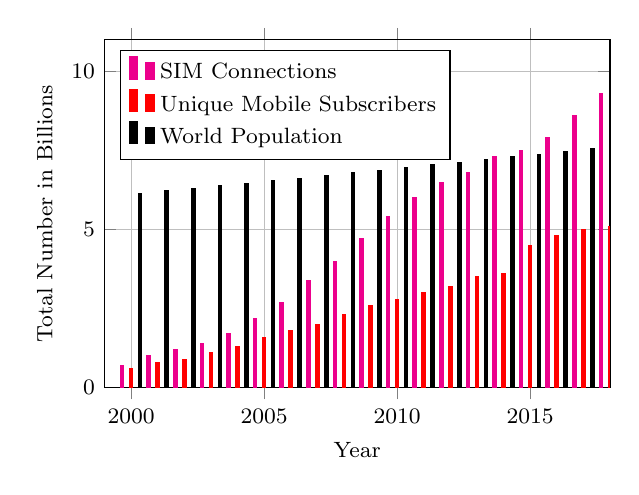
\begin{tikzpicture}
\begin{axis}[
  width=8cm,
  height=6cm,
  font=\footnotesize,
  ybar,
  bar width=1.25pt,
  xlabel={Year},
  ylabel={Total Number in Billions},
  xmajorgrids,
  ymajorgrids,
  ymin=0,
  ymax=11,
  xmin=1999,
  xmax=2018,
  xtick={2000,2005,2010,2015},
  x tick label style={/pgf/number format/.cd,set thousands separator={}},
  legend entries={SIM Connections,Unique Mobile Subscribers,World Population},
  legend style={legend pos=north west,nodes=right}]
\addplot [
color=magenta,
fill=magenta
]
coordinates{
(2000,0.7)
(2001,1.0)
(2002,1.2)
(2003,1.4)
(2004,1.7)
(2005,2.2)
(2006,2.7)
(2007,3.4)
(2008,4.0)
(2009,4.7)
(2010,5.4)
(2011,6.0)
(2012,6.5)
(2013,6.8)
(2014,7.3)
(2015,7.5)
(2016,7.9)
(2017,8.6)
(2018,9.3)
};

\addplot [
color=red,
fill=red
]
coordinates{
(2000,0.6)
(2001,0.8)
(2002,0.9)
(2003,1.1)
(2004,1.3)
(2005,1.6)
(2006,1.8)
(2007,2.0)
(2008,2.3)
(2009,2.6)
(2010,2.8)
(2011,3.0)
(2012,3.2)
(2013,3.5)
(2014,3.6)
(2015,4.5)
(2016,4.8)
(2017,5.0)
(2018,5.1)
};
\addplot [
color=black,
fill=black,
]
coordinates{
(2000,6.143493823)
(2001,6.222626606)
(2002,6.301773188)
(2003,6.381185114)
(2004,6.461159389)
(2005,6.541907027)
(2006,6.623517833)
(2007,6.705946610)
(2008,6.789088686)
(2009,6.872767093)
(2010,6.956823603)
(2011,7.041194301)
(2012,7.125828059)
(2013,7.210581976)
(2014,7.295290765)
(2015,7.379797139)
(2016,7.464022049)
(2017,7.547858925)
(2018,7.631091040)
%(2019,7.713468100)
};

\end{axis}
\end{tikzpicture}
 \\
  {\tiny \textcolor{gray}{Sources: United Nations, GSMA}}
  \end{center}
\column{.22\textwidth}
  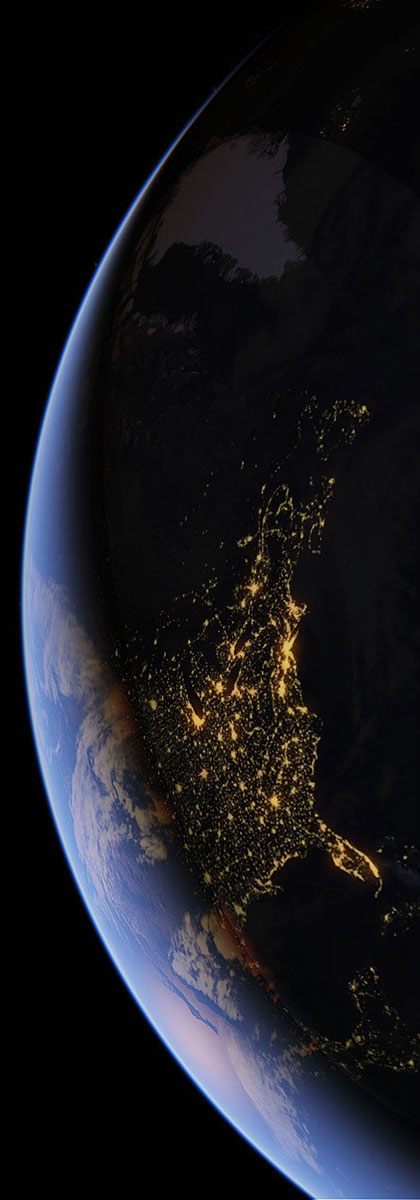
\includegraphics[height=7.2cm]{Figures/Visual-Earth.jpg} \\
  {\tiny \textcolor{gray}{\textcopyright Google Earth}}
\end{columns}
\end{frame}


\begin{frame}
\frametitle{Clarity of Vision -- Reaching the Limit}
\begin{columns}
\column{.45\textwidth}
  \begin{center}
  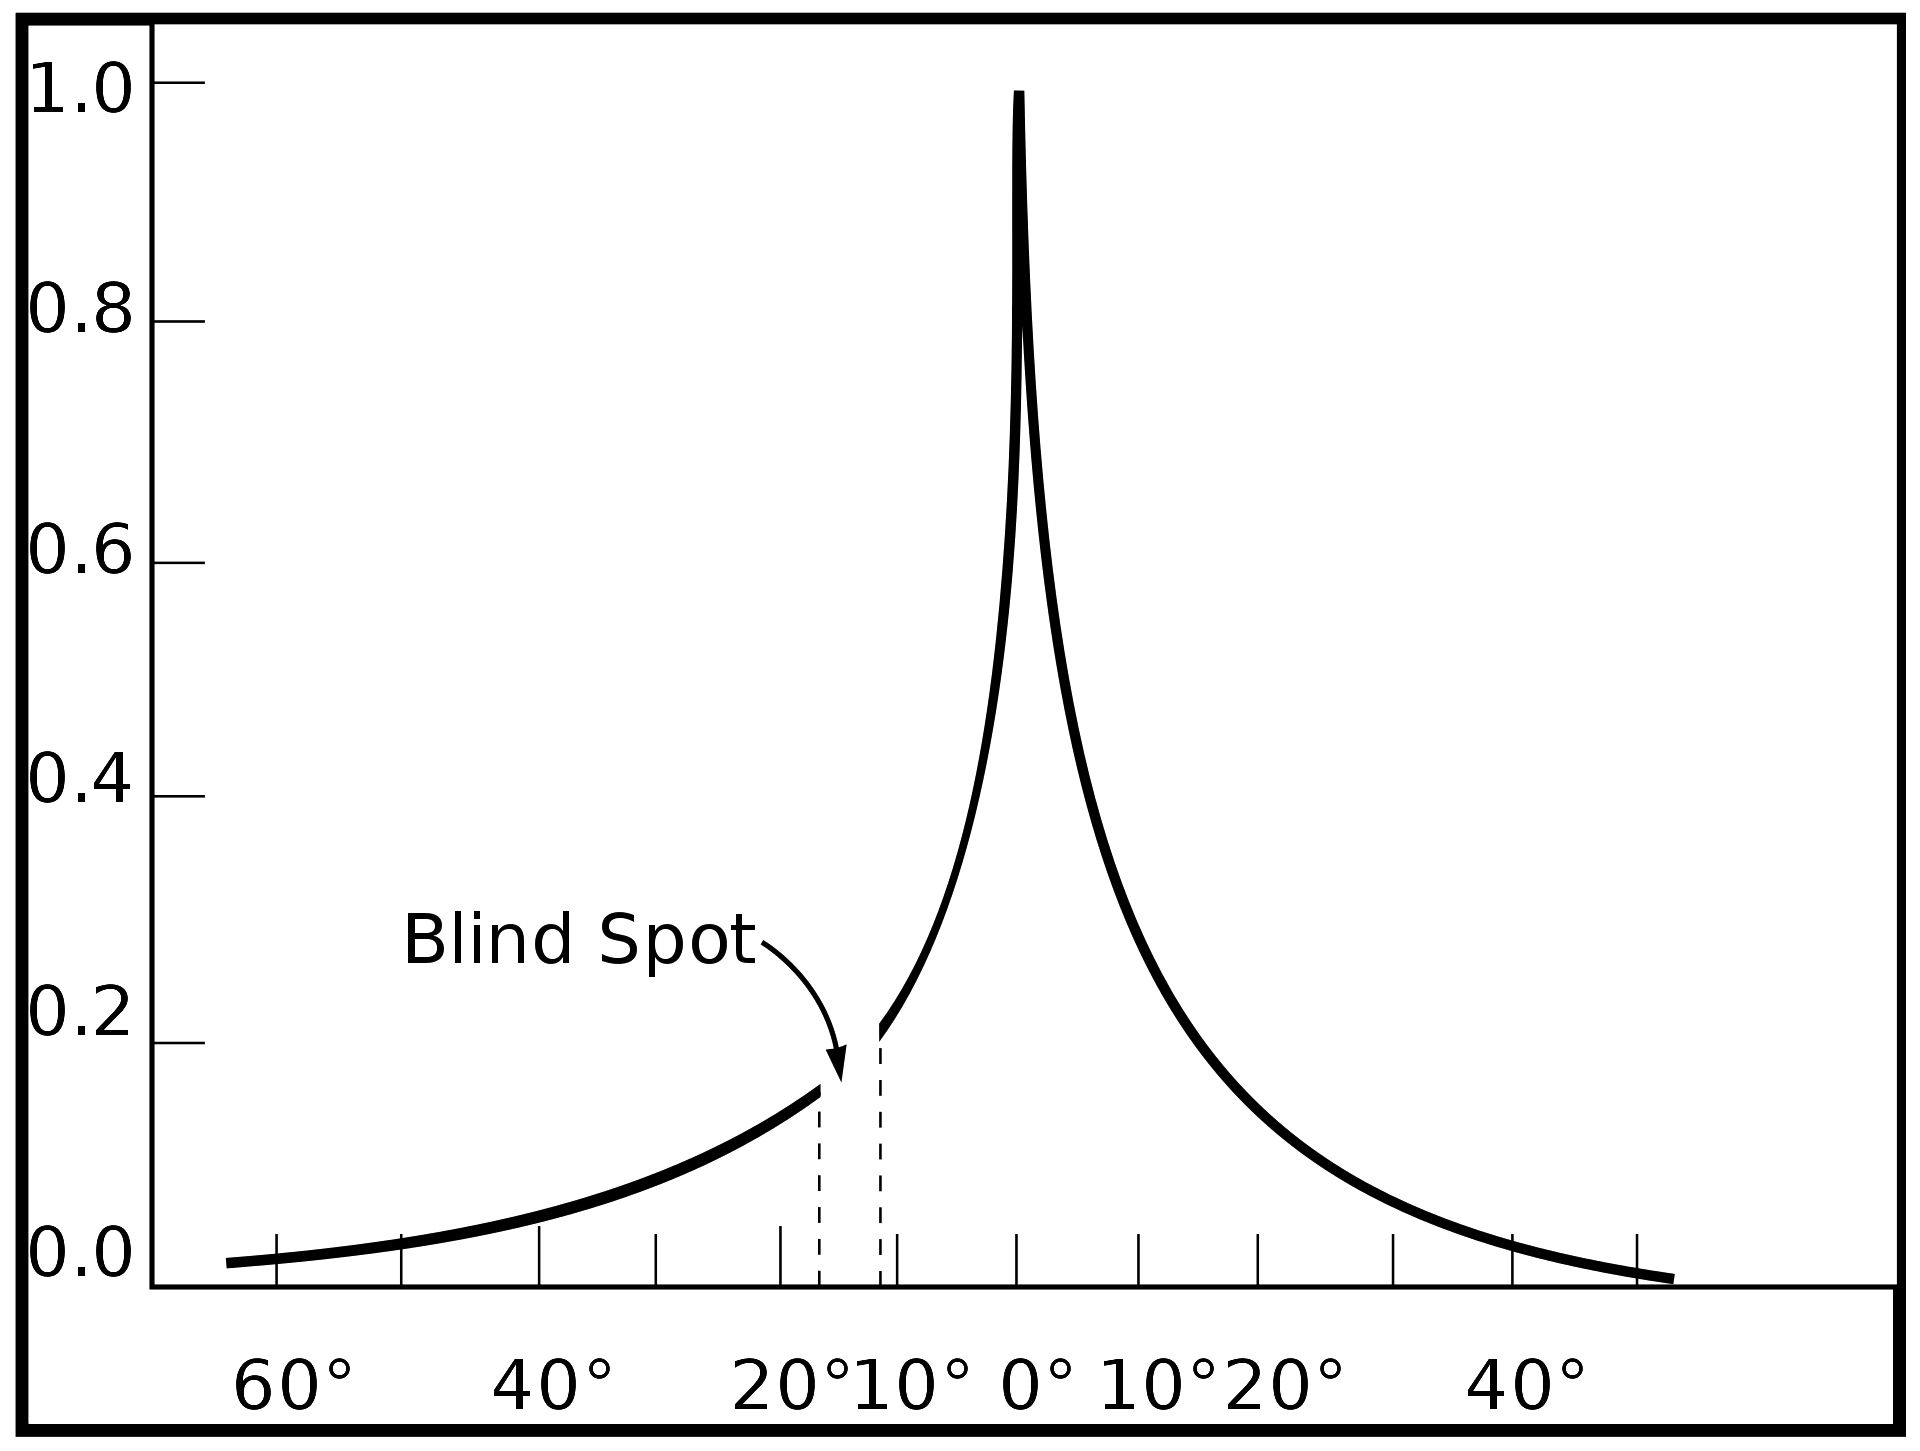
\includegraphics[width=1.5in]{Figures/Visual-Acuity.png}
  \newline
  {\tiny \textcolor{gray}{\textcopyright Vanessa Ezekowitz}}
  \vspace{5mm}
  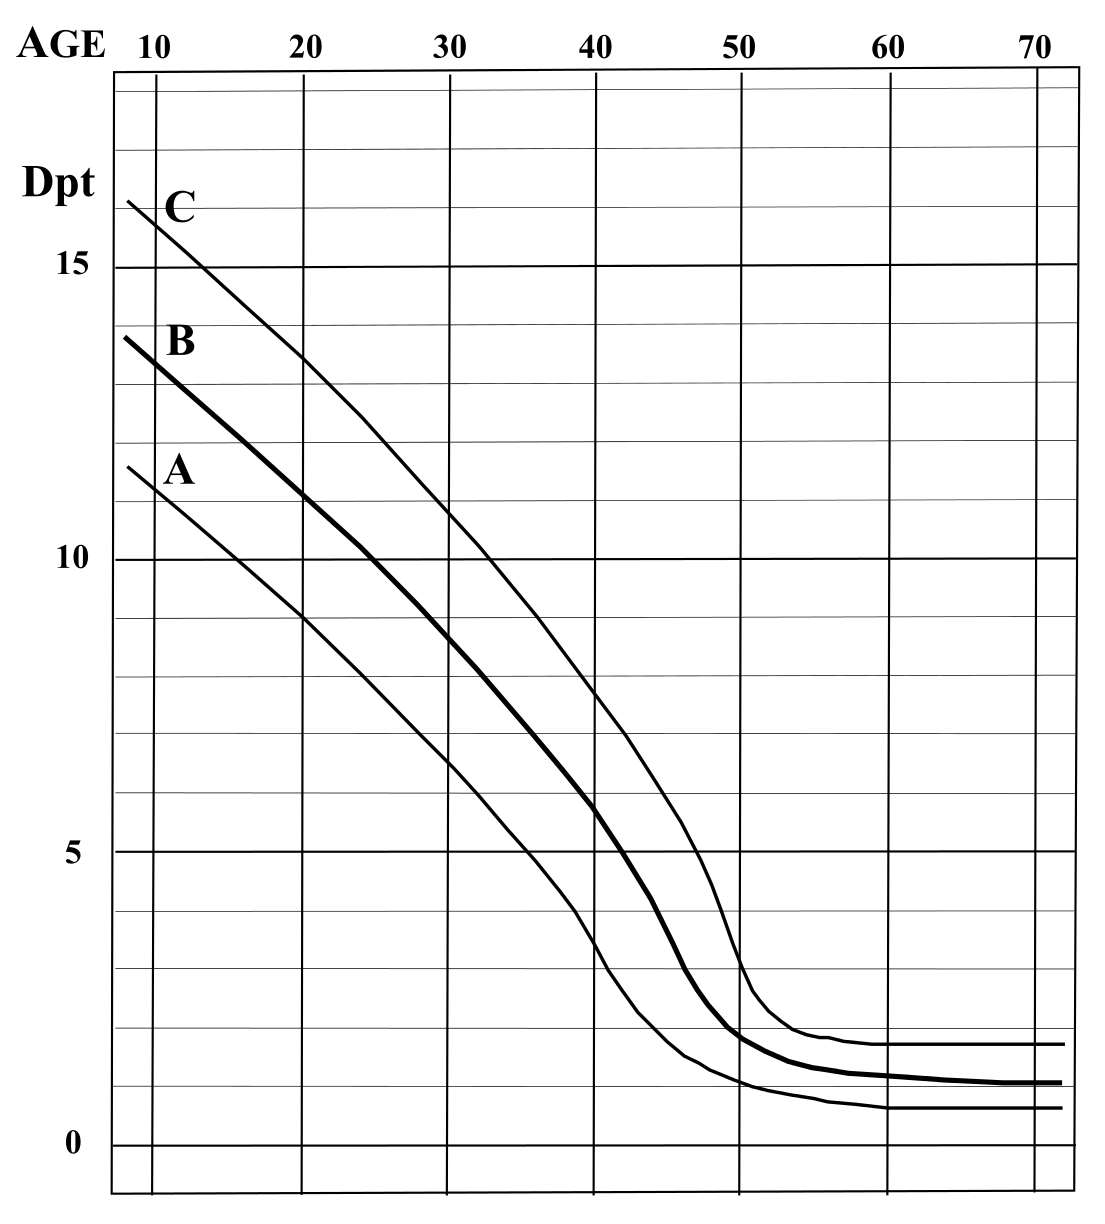
\includegraphics[width=1.5in, height=1.25in]{Figures/Visual-Accommodation.png}
  \newline
  {\tiny \textcolor{gray}{\textcopyright Hans Strasburge}}
  \end{center}
\column{.5\textwidth}
  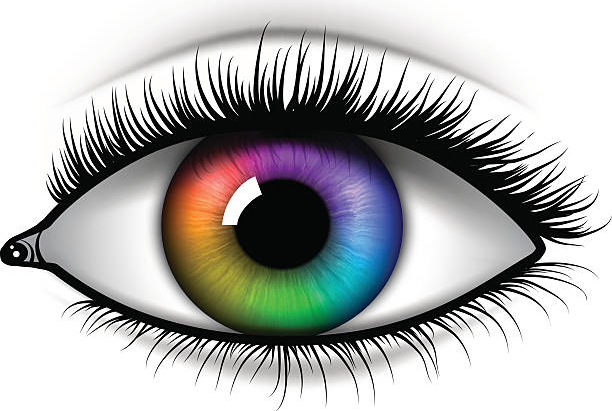
\includegraphics[width=0.75in]{Figures/Visual-HumanEye.png}
  {\tiny \textcolor{gray}{\textcopyright Samarskaya}}
\begin{block}{Visual Resolution}
  Peak visual resolution of $20/20$ human is
  \begin{footnotesize}
  \begin{equation*}
  \begin{split}
  &\frac{1}{\text{Visual Acuity}}
  = \frac{1}{20/20}~\text{min. of arc} \\
  %&= \frac{1}{60}~\text{degrees}
  &\approx 0.0167~\text{degrees}
  \end{split}
  \end{equation*}
  \end{footnotesize}
  Sharp drops limit viewing angle to $\pm 20$~degrees
\end{block}
\begin{block}{Amplitude of Accommodation}
  Diopters capture eye adaptability in reciprocal of focal length,
  Crystalline limits minimum range
\end{block}
\end{columns}
\end{frame}


\begin{frame}
\frametitle{Visual Acuity and Display Technology}
\begin{columns}
\column{.30\textwidth}
  \begin{center}
  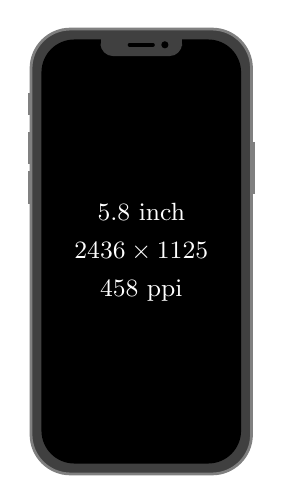
\begin{tikzpicture}
  [
  font=\small,
  line width=1pt,
  draw=black, >=stealth',
  bitnode/.style={circle, inner sep = 0pt, minimum size = 6mm, draw=black},
  checknode/.style={rectangle, inner sep = 0pt, minimum size = 6mm, draw=black},
  ]

\draw[draw=gray,fill=darkgray,rounded corners=0.5cm] (-1.4,-2.825) rectangle (1.4,2.825);
\draw[draw=black,fill=black,rounded corners=0.4cm] (-1.25,-2.675) rectangle (1.25,2.675);
\draw[draw=darkgray,fill=darkgray,rounded corners] (-0.5,2.5) rectangle (0.5,2.75);
\draw[draw=darkgray,fill=darkgray] (-0.5,2.625) rectangle (0.5,2.75);
\draw[draw=black,line width=1.25pt,line cap=round] (-0.15,2.625) -- (0.15,2.625);
\draw[draw=black,fill=black] (0.3,2.625) circle (0.75pt);

\node[text=white] at (0,0.5) {$5.8$~inch};
\node[text=white] at (0,0) {$2436 \times 1125$};
\node[text=white] at (0,-0.5) {$458$~ppi};

\draw[draw=gray,fill=gray] (-1.425,2) rectangle (-1.4,1.75);
\draw[draw=gray,fill=gray] (-1.425,1.5) rectangle (-1.4,1.125);
\draw[draw=gray,fill=gray] (-1.425,1.0) rectangle (-1.4,0.625);
\draw[draw=gray,fill=gray] (1.425,1.375) rectangle (1.4,0.75);
\end{tikzpicture}

  \newline
  {\tiny \textcolor{gray}{Apple Super Retina HD}}
  \end{center}
\column{.65\textwidth}
\begin{block}{Screen Distance}
  The distance at which the super retina HD display matches this resolution is
  \begin{small}
  \begin{equation*}
  \begin{split}
  \text{Distance} &= \frac{1}{2} \cdot \frac{1}{458} \cdot \cot \frac{1}{120} \\
  &= 1.876~\text{in} .
  \end{split}
  \end{equation*}
  \end{small}
\end{block}
\begin{block}{Mobile VR Headsets}
  \begin{center}
  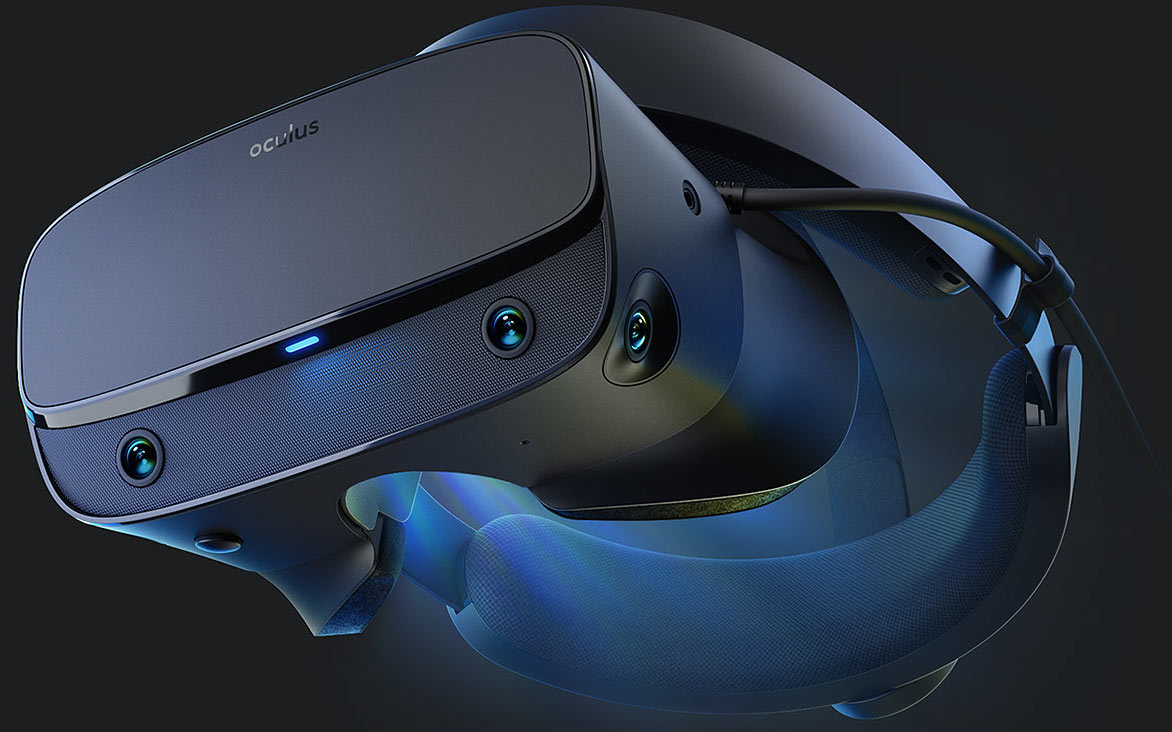
\includegraphics[width=2in]{Figures/Visual-Oculus.jpg}
  \newline
  {\tiny \textcolor{gray}{\textcopyright Oculus Rift}}
  \end{center}
  \end{block}
\end{columns}
\end{frame}


\begin{frame}
\frametitle{Content-Rich Applications}
\begin{center}
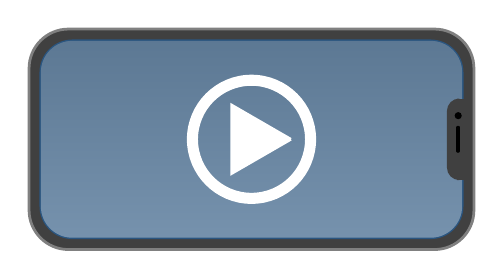
\begin{tikzpicture}
  [font=\small, line width=1pt, draw=black, >=stealth']

\draw[draw=gray,fill=darkgray,rounded corners=0.5cm] (-2.825,-1.4) rectangle (2.825,1.4);
\draw[draw={rgb:red,1;green,2;blue,3},fill={rgb:red,1;green,2;blue,3},rounded corners=0.4cm] (-2.675,-1.25) rectangle (2.675,1.25);
\shade[fill=white, fill opacity=0.2,rounded corners=0.4cm] (-2.675,-1.25) rectangle (2.675,1.25);

\draw[draw=darkgray,fill=darkgray,rounded corners] (2.5,-0.5) rectangle (2.75,0.5);
\draw[draw=darkgray,fill=darkgray] (2.625,-0.5) rectangle (2.75,0.5);

\draw[draw=black,line width=1.25pt,line cap=round] (2.625,-0.15) -- (2.625,0.15);
\draw[draw=black,fill=black] (2.625,0.3) circle (0.75pt);

\draw[draw=white,line width=4pt] (0,0) circle (0.75);
\draw[draw=white,fill=white] (0.5,0) -- (-0.25,0.433) -- (-0.25,-0.433) -- (0.5,0);
\end{tikzpicture}

\end{center}
\begin{columns}
\column{.65\textwidth}
\begin{block}{Video and Mobile Statistics}
  \begin{itemize}
  \item 63\% of all US online traffic comes from smartphones and tablets
    {\tiny \textcolor{gray}{--~Stone Temple}}
  \item More than 70\% of YouTube viewing happens on mobile devices
    {\tiny \textcolor{gray}{--~Comscore}}
  \item 65\% of all digital media time is spent on mobile devices
    {\tiny \textcolor{gray}{--~Business2Community}}
  \end{itemize}
\end{block}
\column{.30\textwidth}
  \begin{center}
  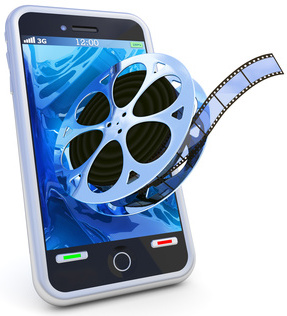
\includegraphics[width=0.96\textwidth]{Figures/Video-Real.jpg}
  \newline
  {\tiny \textcolor{gray}{\textcopyright Real}}
  \end{center}
\end{columns}
\end{frame}


\begin{frame}
\frametitle{Options to Stay the Course}
  \textbf{Spend More Time on Mobile Devices}\newline
  Average time spent on mobile phone in US is 3h45m per day \\
  {\tiny \textcolor{gray}{-- eMarketer}}
\begin{columns}
\column{.30\textwidth}
  
\includegraphics[width=.96\textwidth]{Figures/Visual-magoo.png}
  \newline
  {\tiny \textcolor{gray}{\textcopyright Dreamworks}}
\column{.65\textwidth}
  \textbf{Wait for Eye Evolution}
  \begin{center}
  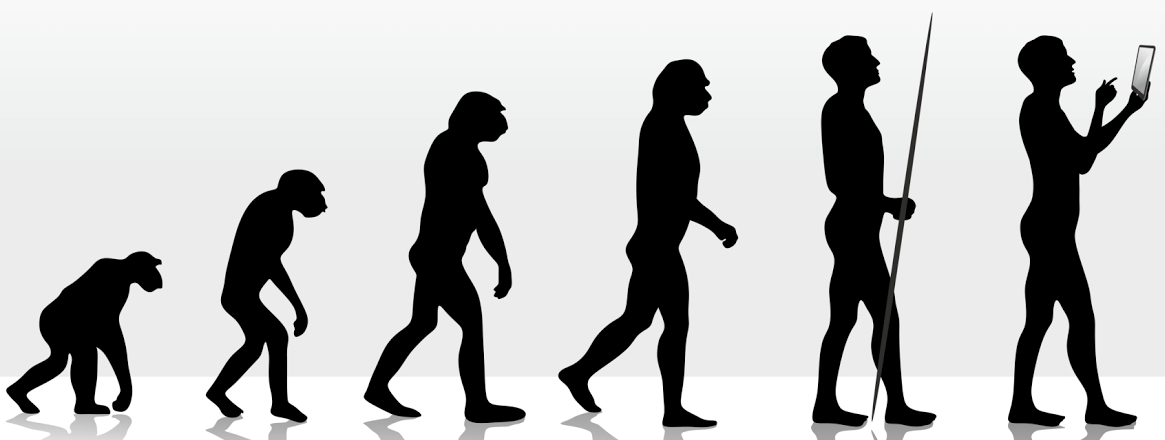
\includegraphics[width=2in]{Figures/Visual-Evolution.png}
  {\tiny \textcolor{gray}{\textcopyright Ravishly}}
  \end{center}
  \textbf{Diversify User Population}
  \begin{center}
  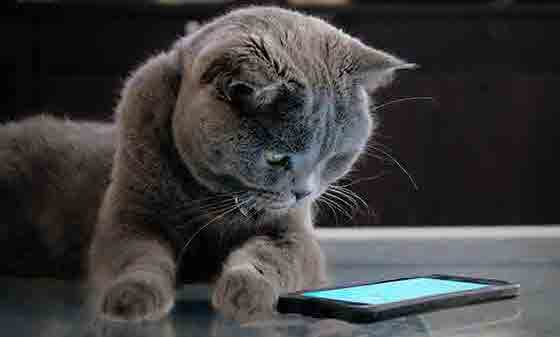
\includegraphics[width=2in]{Figures/Visual-Animals.jpg}
  {\tiny \textcolor{gray}{\textcopyright Asurobson}}
  \end{center}
\end{columns}
\end{frame}


\begin{frame}
\frametitle{Summary of Quality of Experience}
\begin{block}{Current Wireless Landscape}
  \begin{itemize}
  \item \textbf{Growth and Market Penetration}: Near saturation
    \begin{itemize}
    \item Number of connected wireless devices exceeds world population
    \item Almost every human who wants mobile phone has one (or more)
    \end{itemize}
  \item \textbf{Screen Quality}: At limit of eye acuity
    \begin{itemize}
    \item Screens are near boundary of visual resolution
    \item Viewing distance is constrained by amplitude of accommodation
    \end{itemize}
  \item \textbf{Content-Rich Apps}: Video watching \& gaming are prevalent
    \begin{itemize}
    \item On average, a person spends 4 hours on mobile device per day
    \item More videos are watch on phones than elsewhere
    \end{itemize}
  \end{itemize}
\end{block}
\begin{block}{Wireless Research and the Future}
  \begin{center}
  \begin{tikzpicture}
  \shade[draw=none,
  left color={rgb:red,1;green,2;blue,3},
  right color=frametitle.fg,
  shading angle=60,
  rounded corners,
  blur shadow={shadow blur steps=5}] (-2.25,-0.625) rectangle (2.25,0.625);
  \shade[fill=white, fill opacity=0.1] (-2.25,-0.625) rectangle (2.25,0.625);
  \node at (0,0) {\textcolor{white}{\Large \textbf{What's Next?}}};
  \end{tikzpicture}
  \end{center}
\end{block}
\end{frame}


\begin{frame}
\frametitle{The Rise of the Machine}
\begin{columns}
\column{.55\textwidth}
  \centering{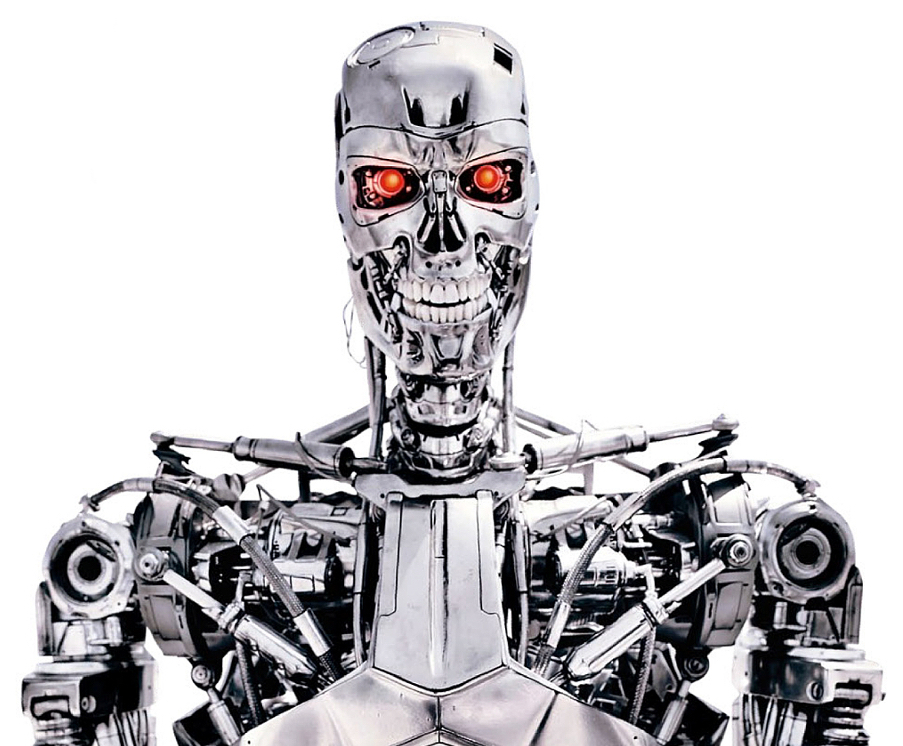
\includegraphics[width=.90\textwidth]{Figures/Machine-Rise.jpg}\newline
  {\tiny \textcolor{gray}{\textcopyright Warner Bros.}}
  \vfill
  \onslide<2->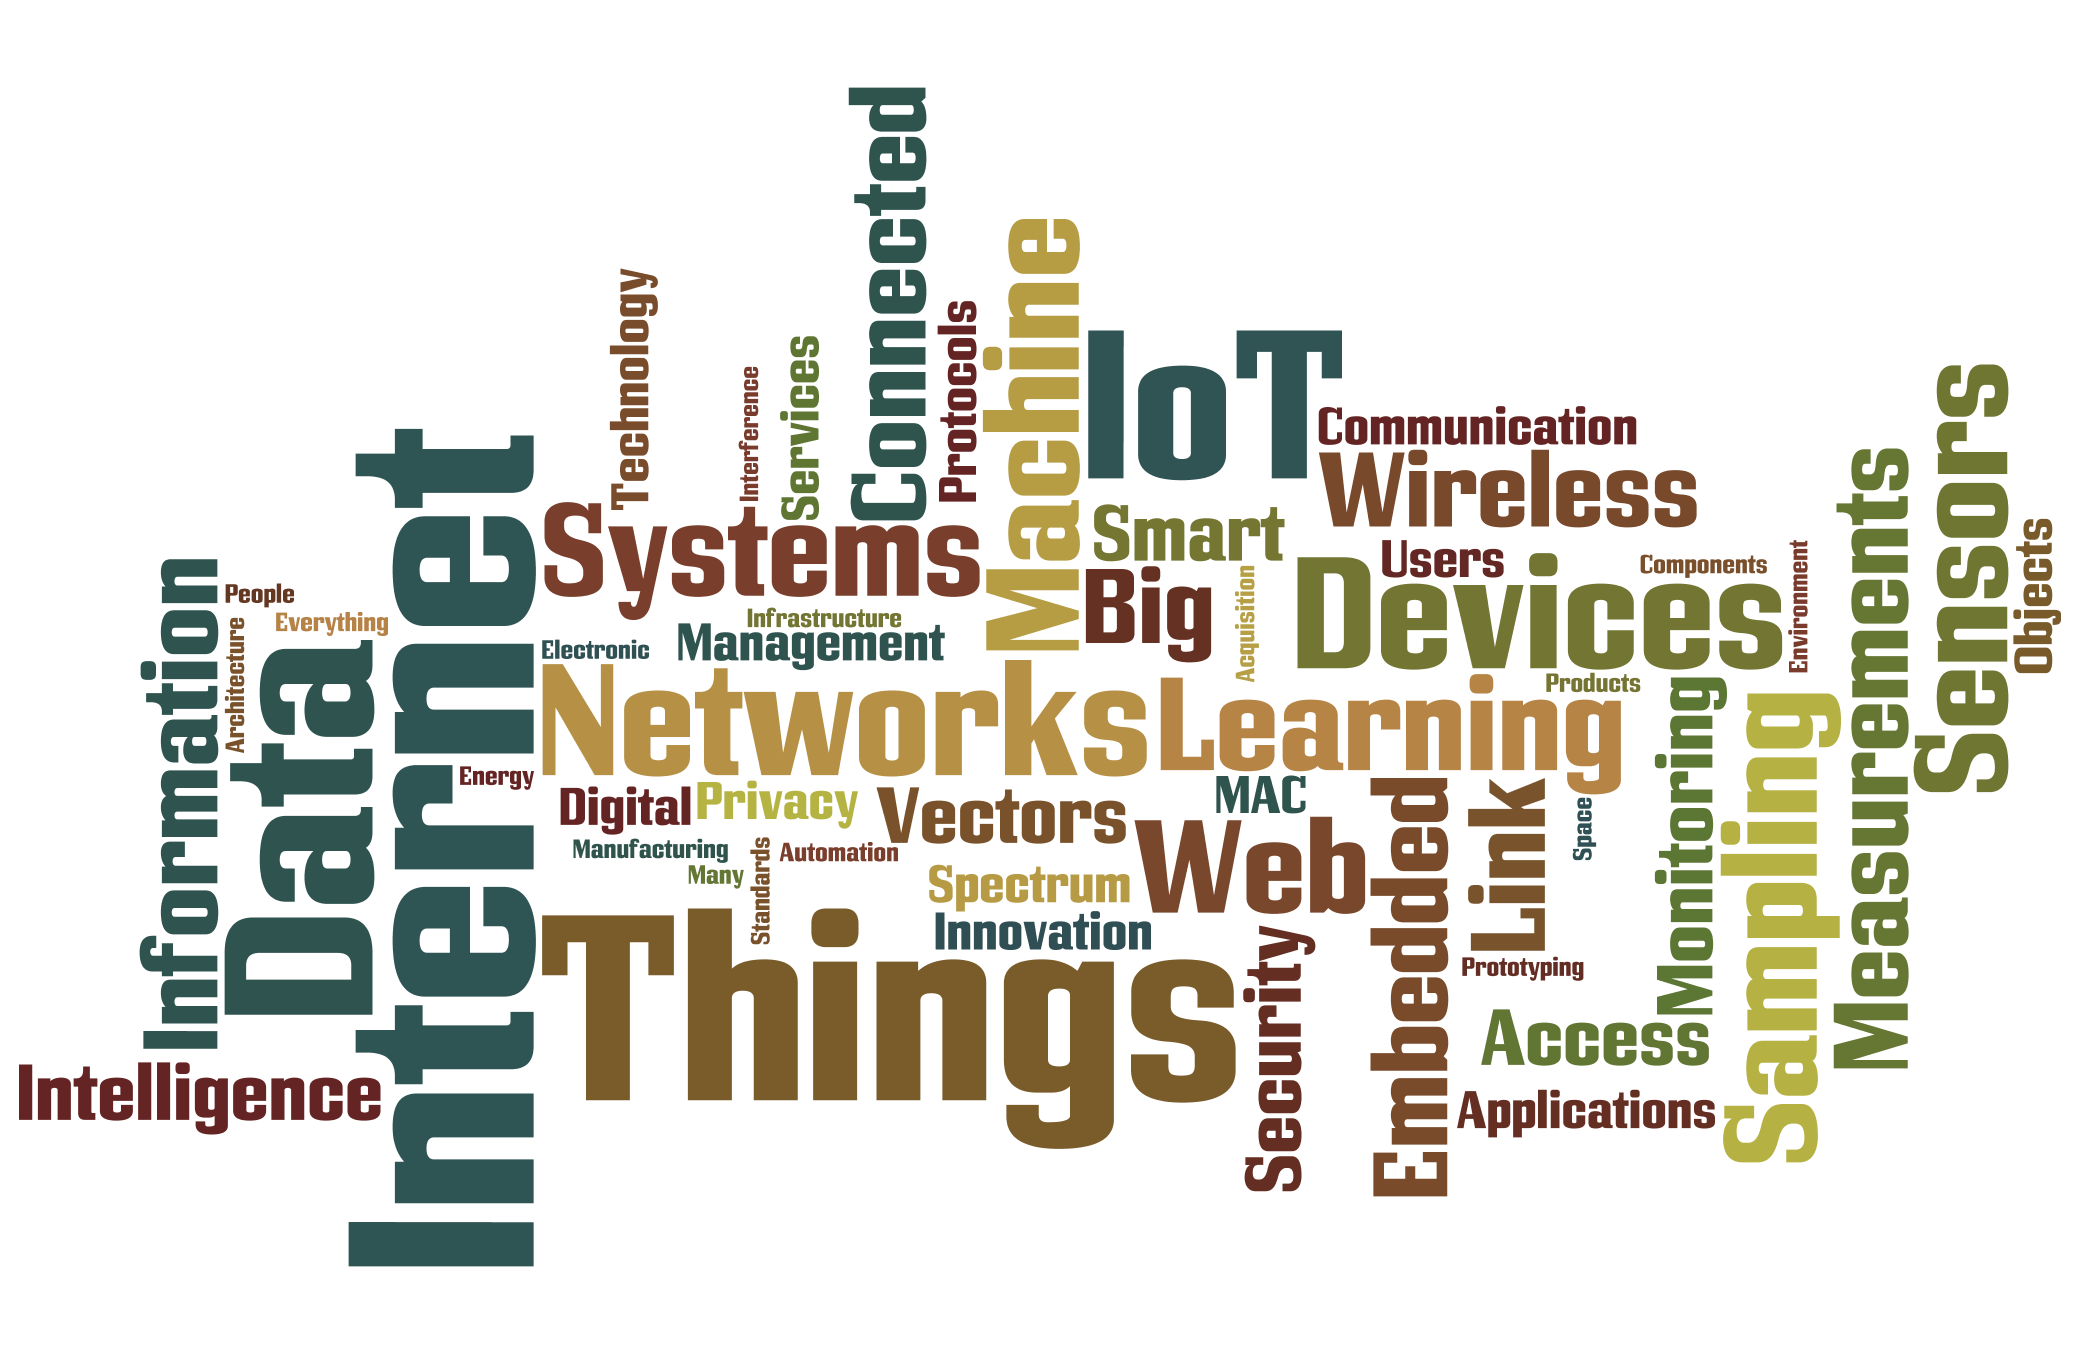
\includegraphics[width=.75\textwidth]{Figures/Wordle.png}}
\column{.5\textwidth}
\onslide<2->\begin{block}{Internet of Things}
  \begin{center}
  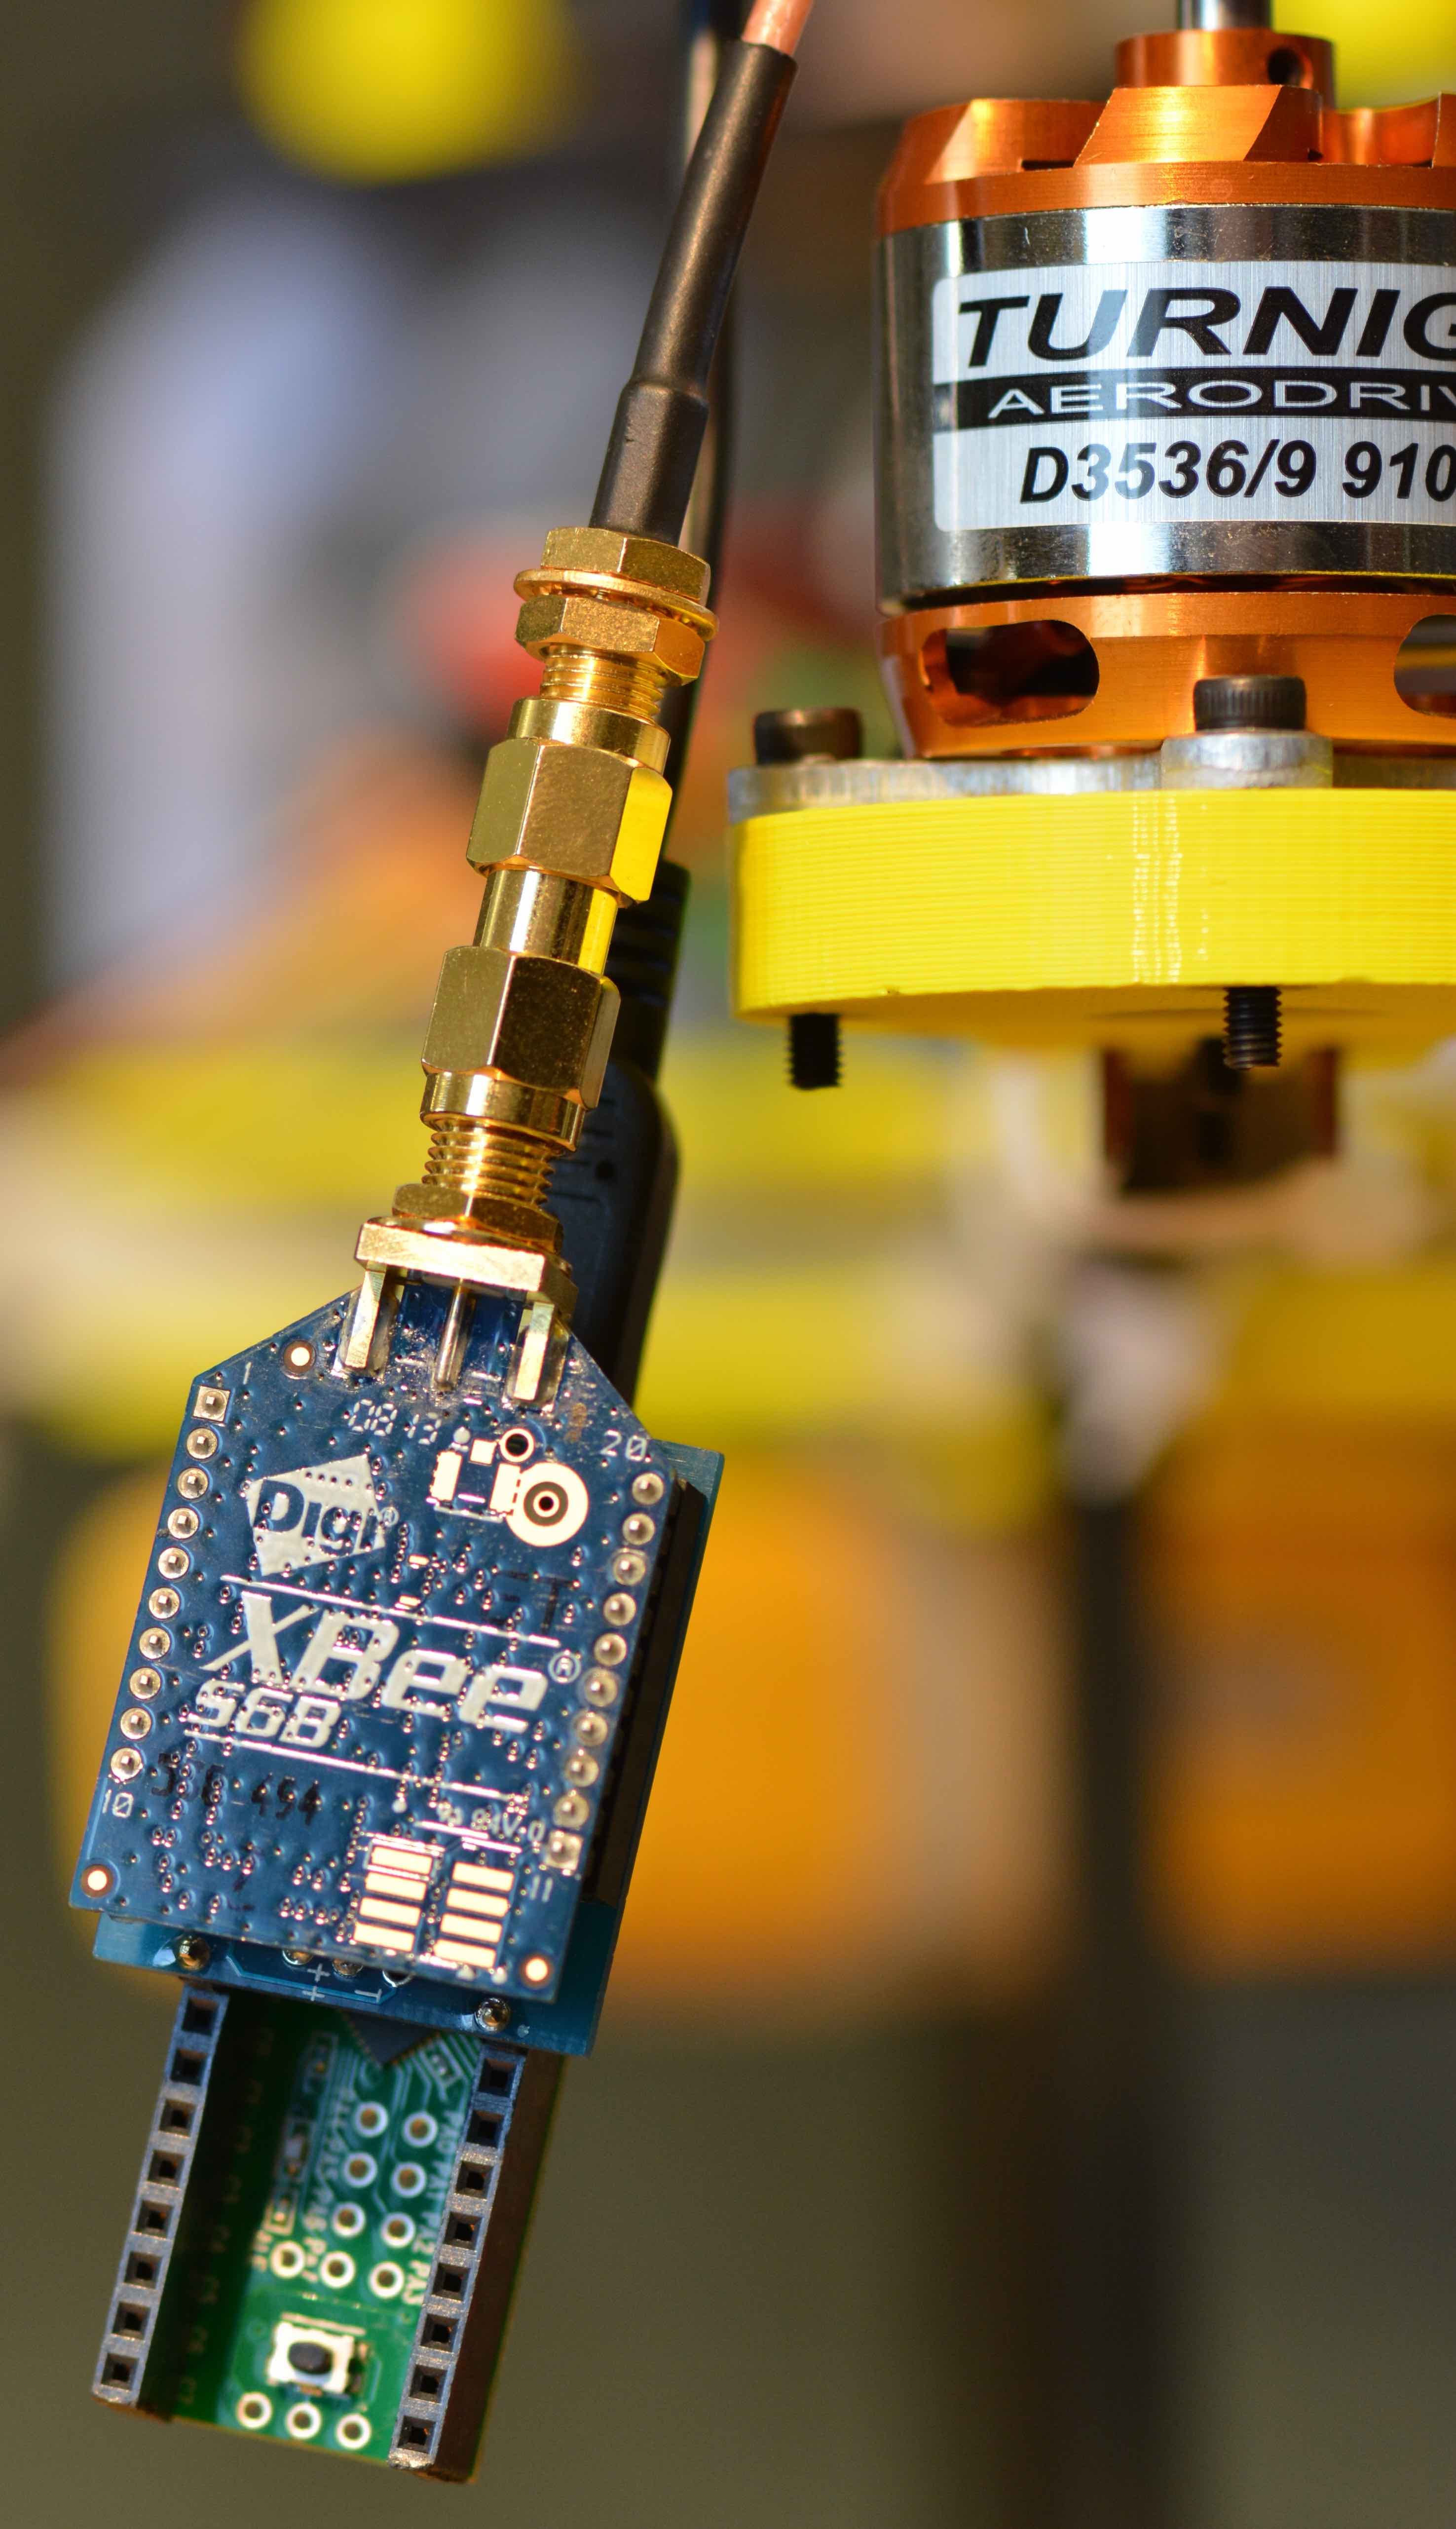
\includegraphics[width=1.5in]{Figures/Machine-Micro.jpg}
  \end{center}
\end{block}
\end{columns}
\end{frame}


\begin{frame}
\frametitle{Contrasting Machines and Human Behaviors}
\begin{columns}
\column{.48\textwidth}
\begin{block}{Typical Human Calendar}
  \begin{itemize}
  \item YouTube video earns 1 view when watched for $\geq 30$~sec
  \item 47\% of visitors expect website to load in $\leq 2$~sec
  \item Callers notice roundtrip voice delays of $\geq 250$~ms
  \end{itemize}
\end{block}


\begin{block}{Machine Scheduler}
  \begin{itemize}
  \item OS timeslice $\approx 10$~ms
  \item LTE schedule $\approx 1$~ms (transmission time interval)
  \item Microcontroller interrupt latency is $\leq 10~\mu$s
  \end{itemize}
\end{block}
\column{.48\textwidth}
  \begin{center}
  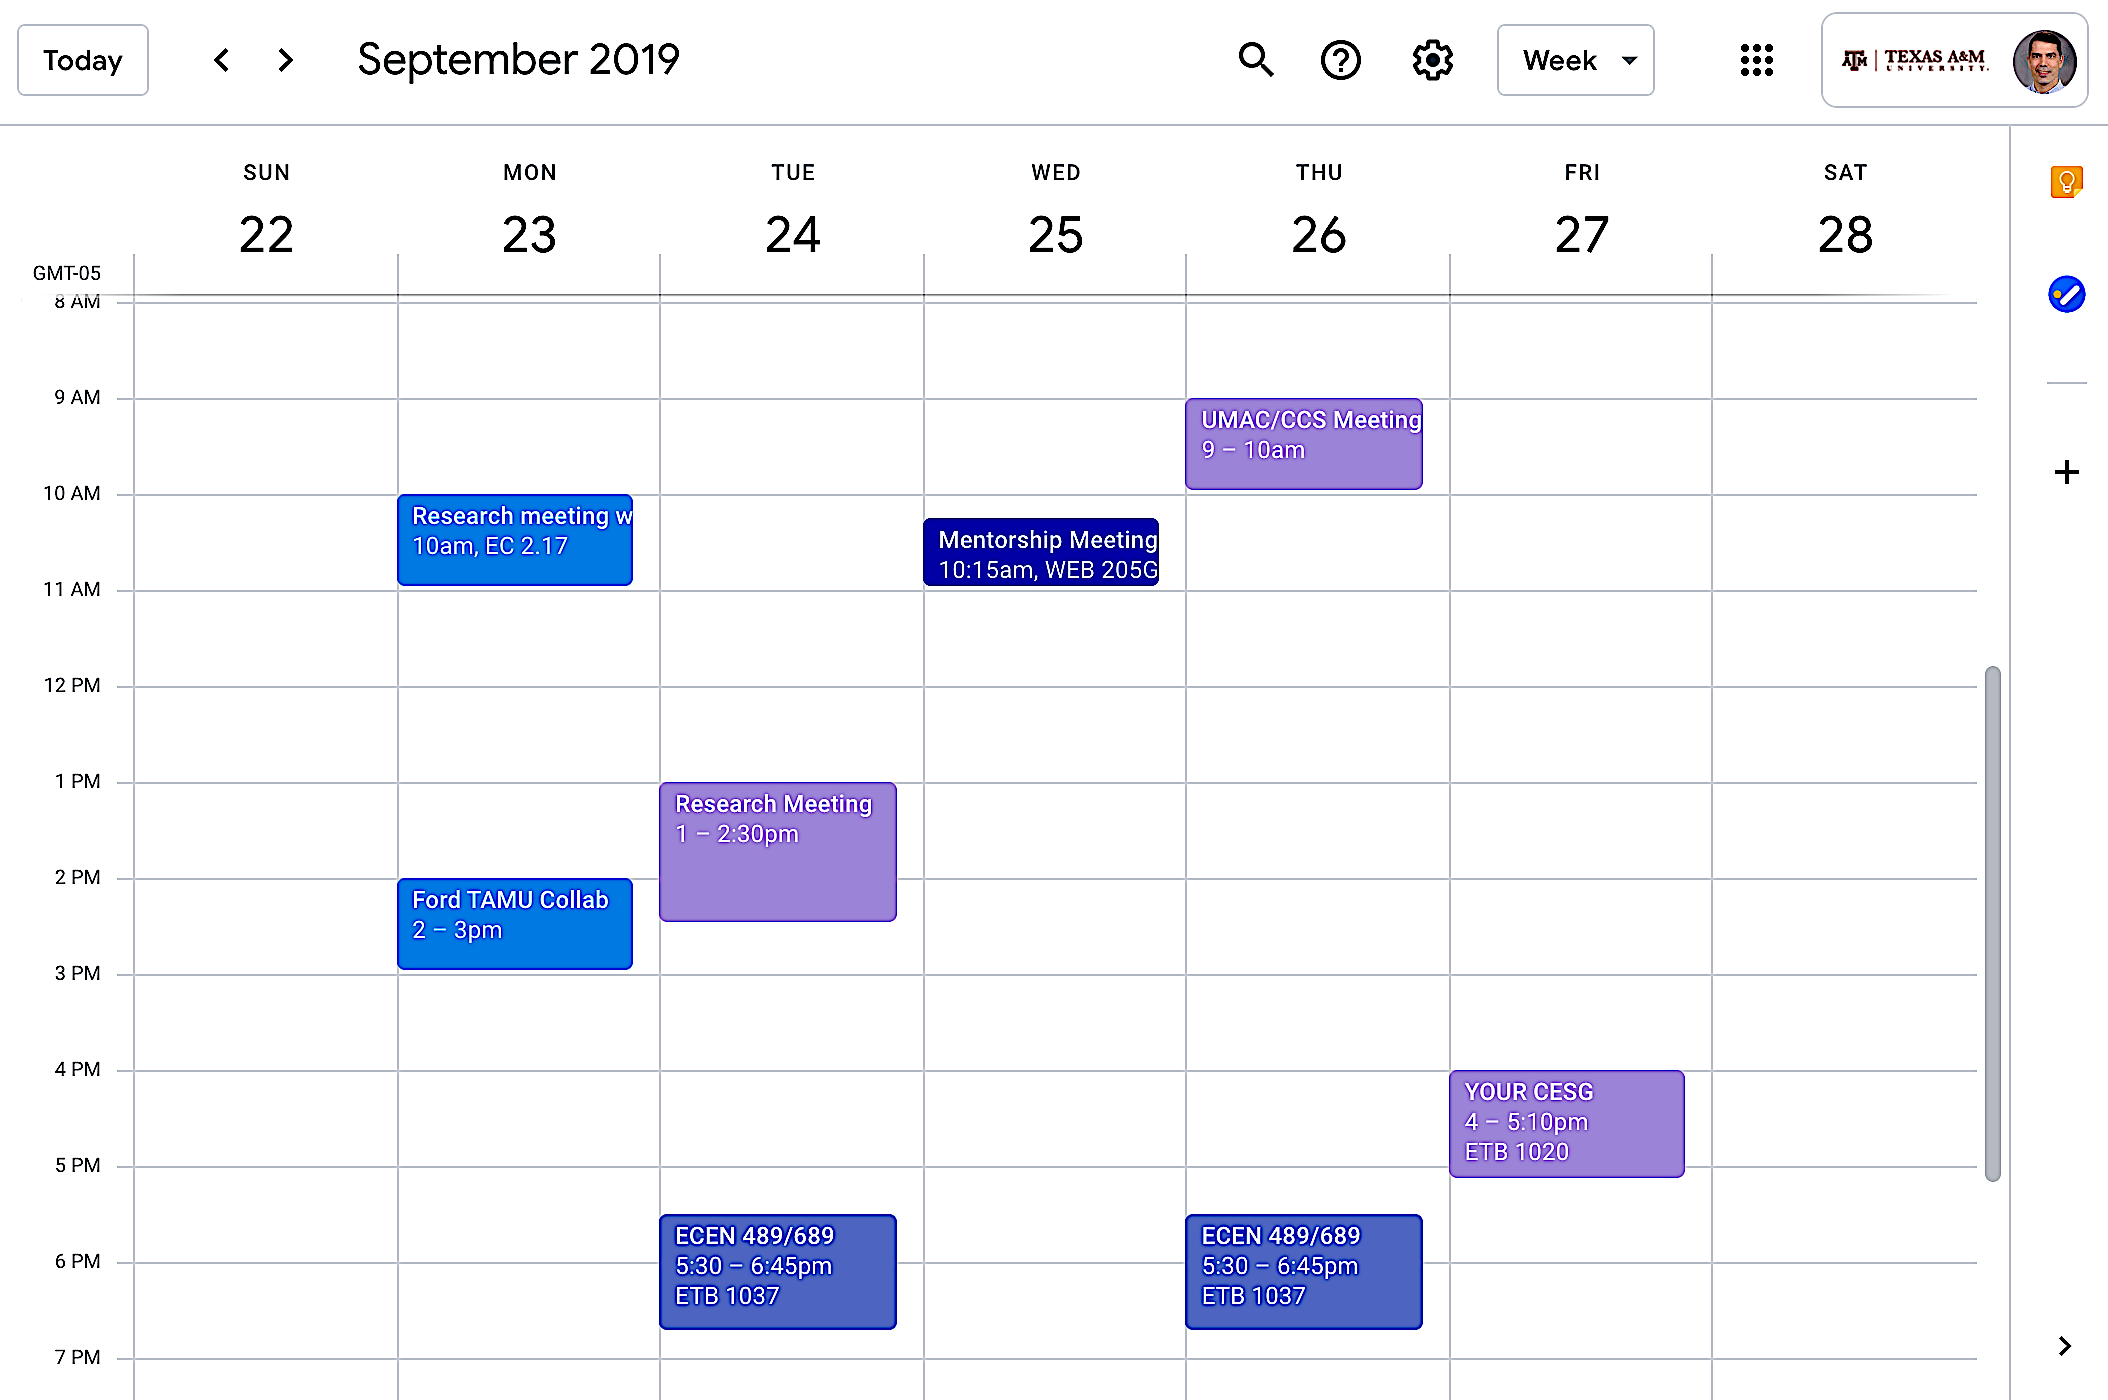
\includegraphics[width=0.95\textwidth]{Figures/Scheduler-Human.png} \\
  \end{center}
  \vfill
  \begin{center}
  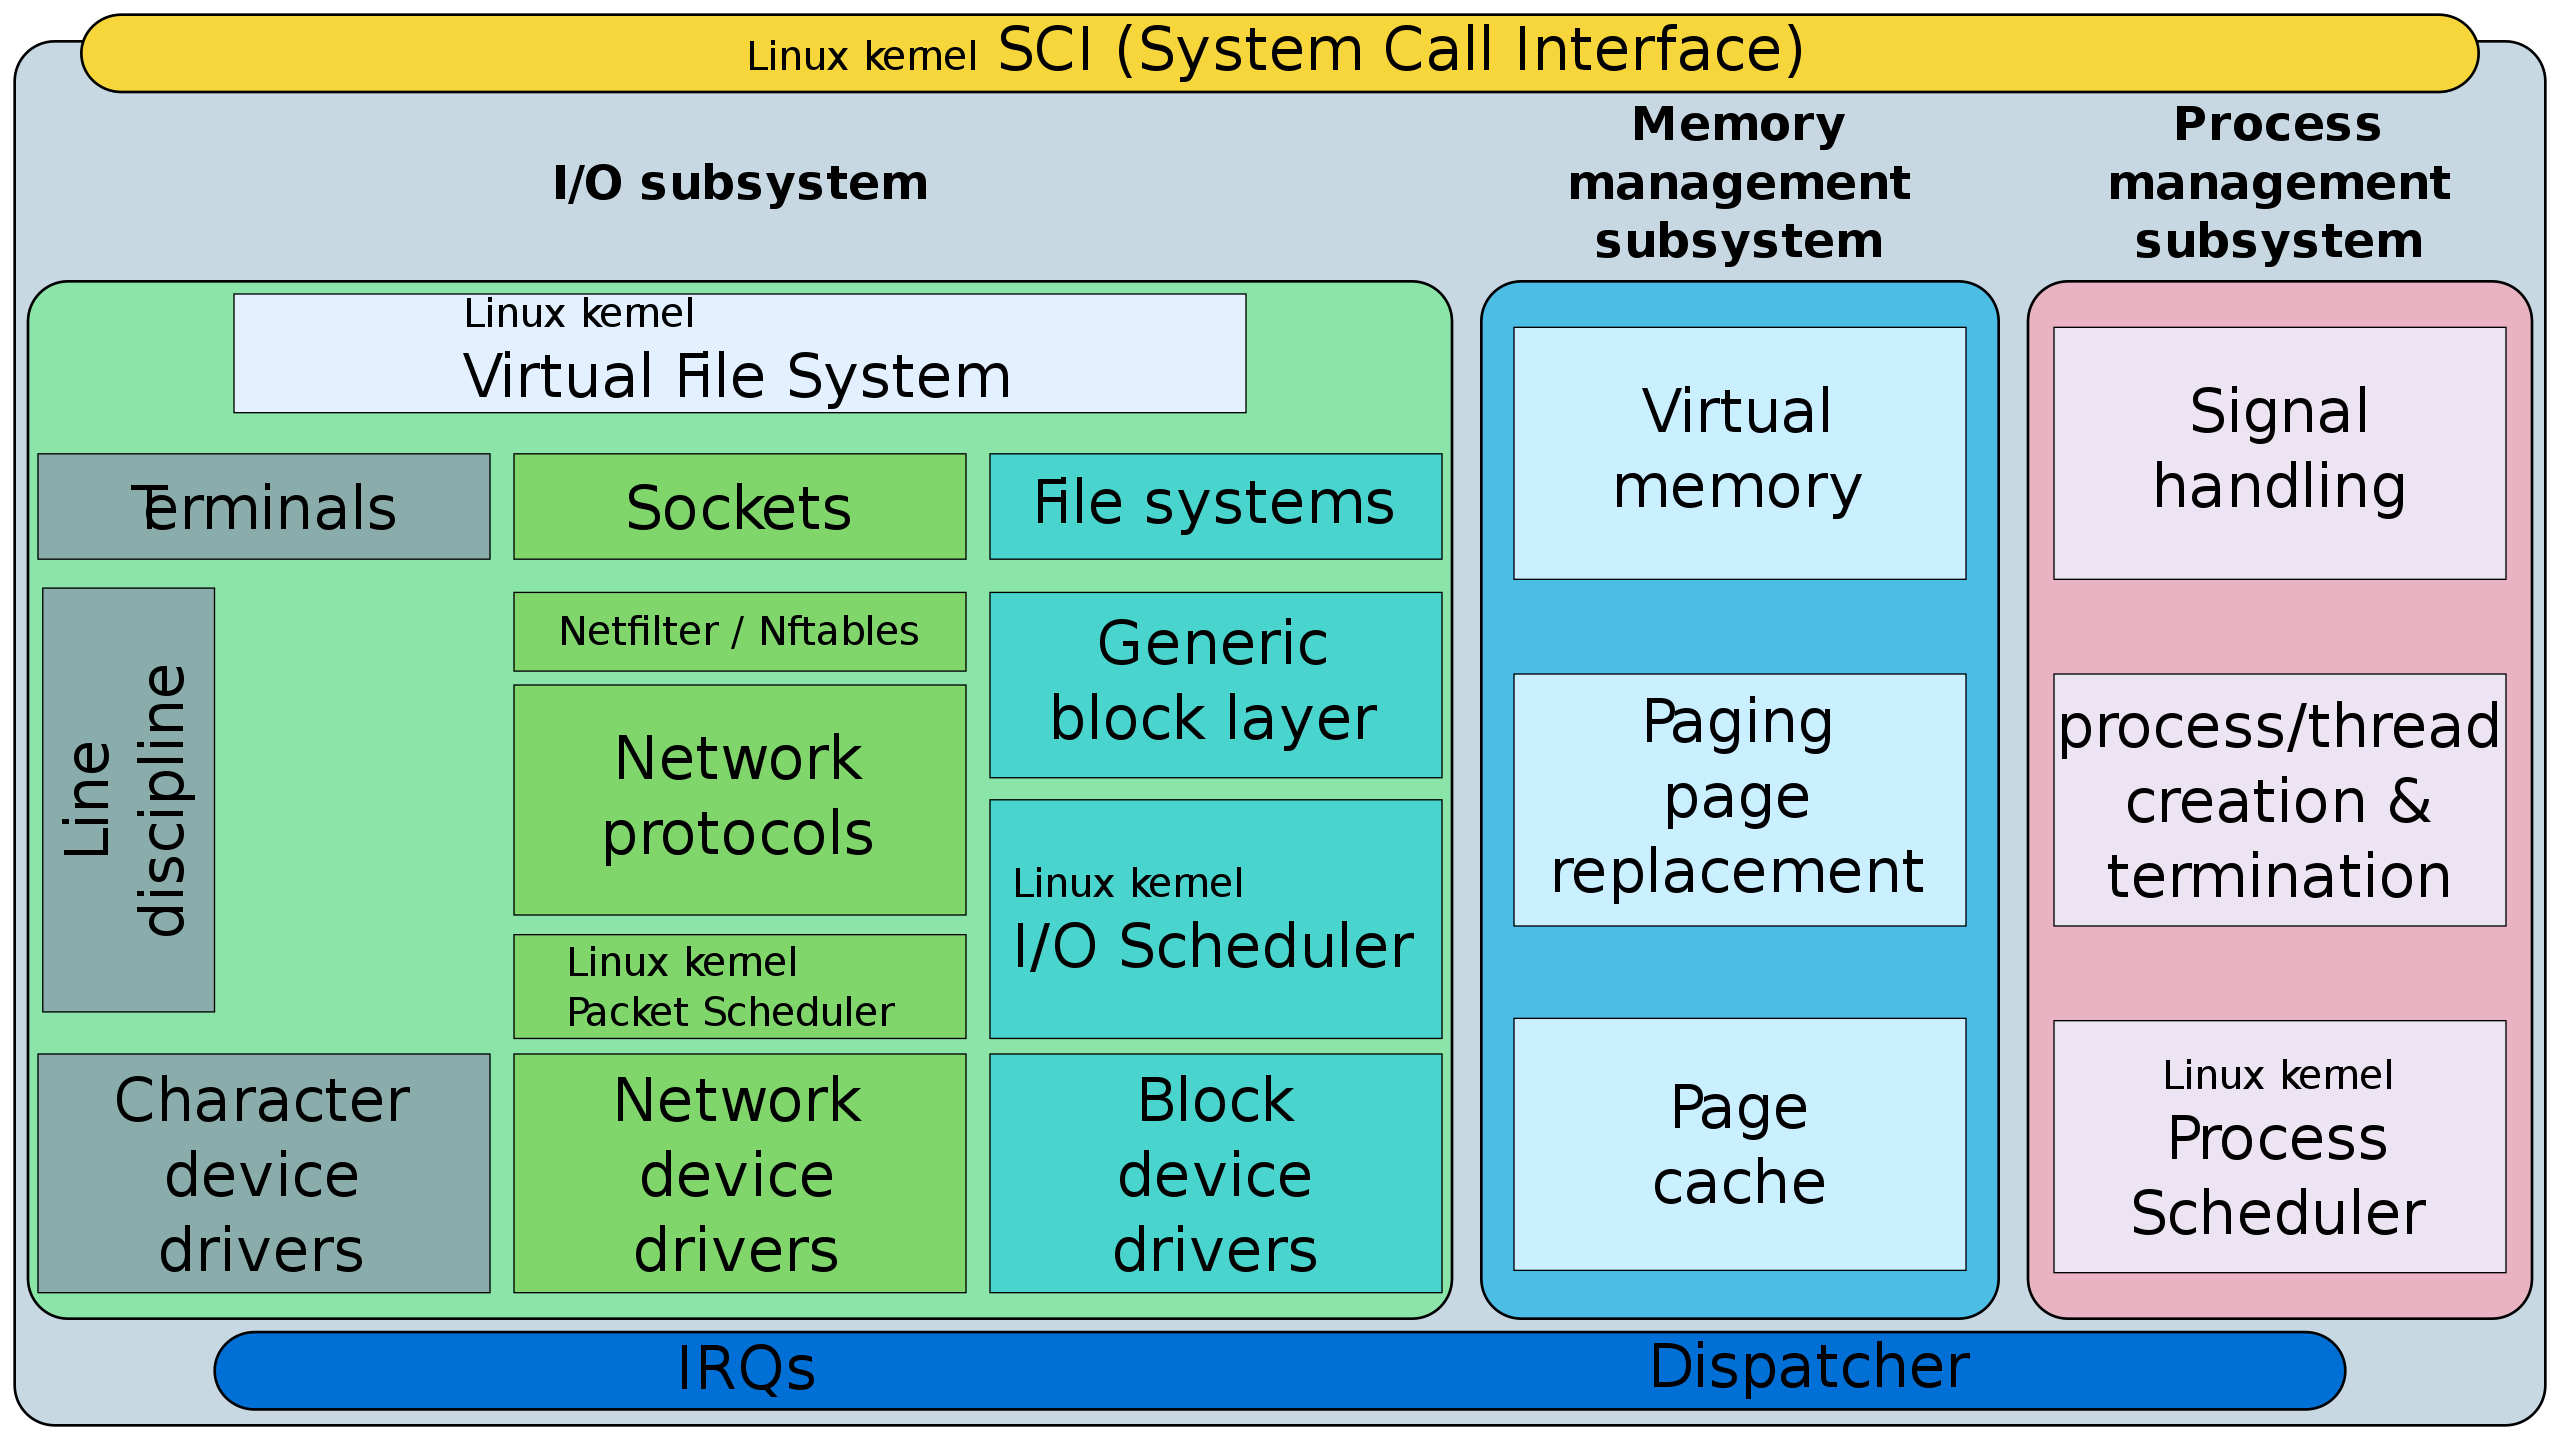
\includegraphics[width=0.95\textwidth]{Figures/Scheduler-Machine.png} \\
  {\tiny \textcolor{gray}{\textcopyright ScotXW}}
  \end{center}
\end{columns}
\end{frame}


\begin{frame}
\frametitle{Information and Inference}
\begin{center}
\begin{tikzpicture}
  \node[scope fading=south] (image) at (0,0) {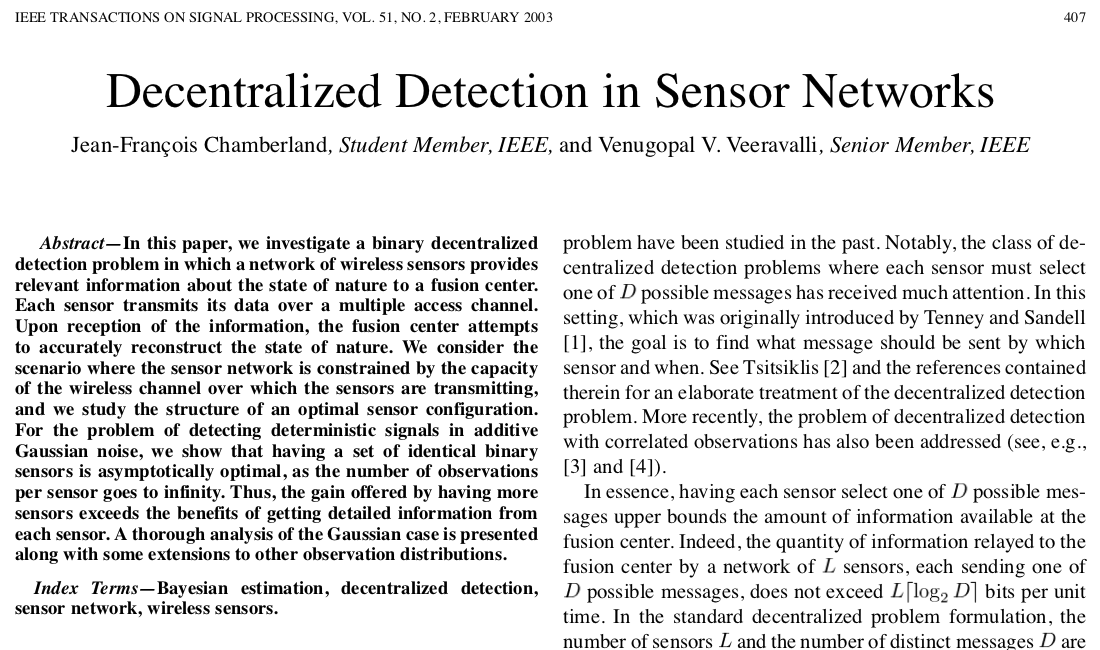
\includegraphics[width=3.5in]{Figures/TSP2002.png}};
\end{tikzpicture}
\end{center}
\vfill
\begin{block}{Payload Design Guideline}
  \begin{itemize}
  \item Most of information for inference is contained in first few bits!
  \end{itemize}
\end{block}
\end{frame}


\begin{frame}
\frametitle{Information and Inference}
\begin{center}
\begin{tikzpicture}
  \node[scope fading=south] (image) at (0,0) {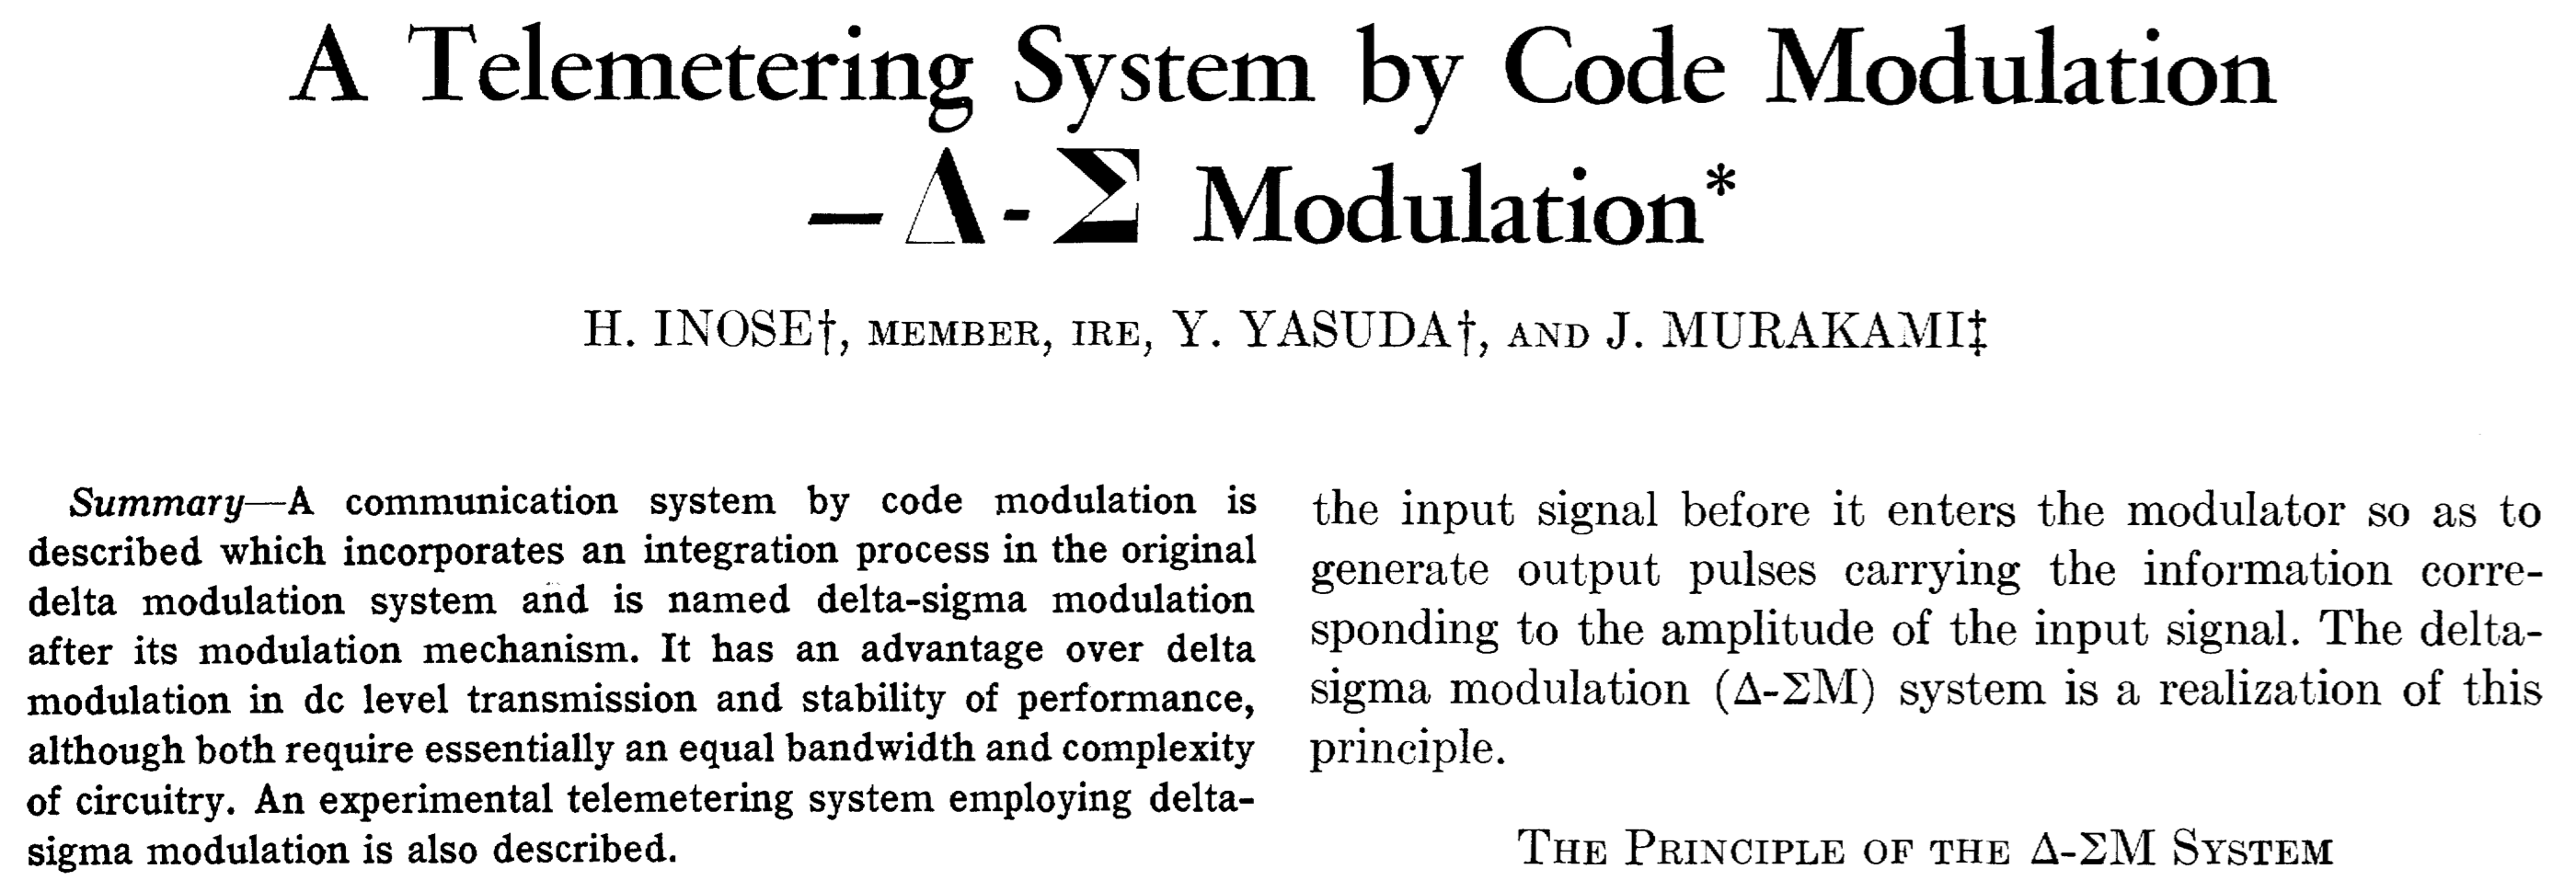
\includegraphics[width=4in]{Figures/SigmaDelta1962.png}};
\end{tikzpicture}
\end{center}
\vfill
\begin{block}{Payload Design Guideline}
  \begin{itemize}
  \item Signals are tracked well using small, yet frequent updates
  \item $\Delta$-$\Sigma$ modulation
  \end{itemize}
\end{block}
\end{frame}


\begin{frame}
\frametitle{Losing the Connection}
\begin{block}{Emerging M2M Traffic Characteristics}
  \begin{itemize}
  \item Device density -- Massive versus small
  \item Connectivity profile -- Sporadic versus sustained
  \item Packet payloads -- Minuscule versus moderate-to-long
  \end{itemize}
\end{block}
\begin{center}
\textbf{Anticipated traffic characteristics invalidate the \emph{acquisition-estimation-scheduling} paradigm!}
\end{center}
\begin{columns}
\column{.45\textwidth}
  \begin{center}
  \scalebox{0.4}{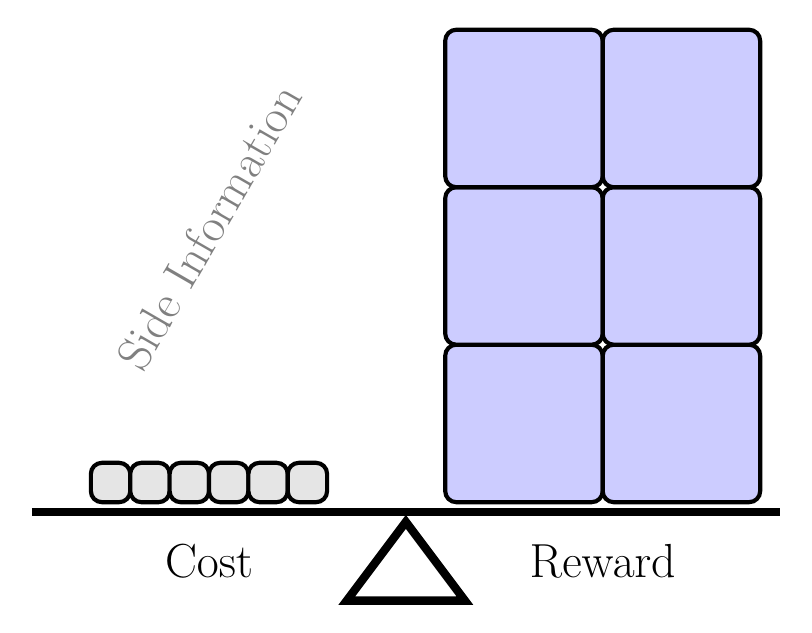
\begin{tikzpicture}
[draw=black, line width=1.5pt, >=stealth',
entry2/.style={rectangle, rounded corners, draw, fill=blue!20, inner sep=0pt, minimum size=20mm},
entry/.style={rectangle, rounded corners, draw, fill=gray!20, inner sep=0pt, minimum size=5mm}]

\node[entry] (r10) at (0.5,0) {};
\node[entry] (r20) at (1,0) {};
\node[entry] (r30) at (1.5,0) {};
\node[entry] (r40) at (2,0) {};
\node[entry] (r50) at (2.5,0) {};
\node[entry] (r60) at (3,0) {};

\node[entry2] (m00) at (5.75,0.75) {};
\node[entry2] (m01) at (5.75,2.75) {};
\node[entry2] (m02) at (5.75,4.75) {};
\node[entry2] (m00) at (7.75,0.75) {};
\node[entry2] (m11) at (7.75,2.75) {};
\node[entry2] (m12) at (7.75,4.75) {};

\draw[line width=3pt] (-0.5,-0.375) -- (9,-0.375);
\draw[line width=3pt] (3.5,-1.5) -- (4.25,-0.5) -- (5,-1.5) -- (3.5,-1.5) -- (4.25,-0.5);

\node (reward) at (1.75,-1) {\LARGE Cost};
\node (cost) at (6.75,-1) {\LARGE Reward};
\node[rotate=60] (info) at (1.75,3.25) {\LARGE \textcolor{gray}{Side Information}};
\end{tikzpicture}
}
  \end{center}
\column{.45\textwidth}
  \begin{center}
  \scalebox{0.4}{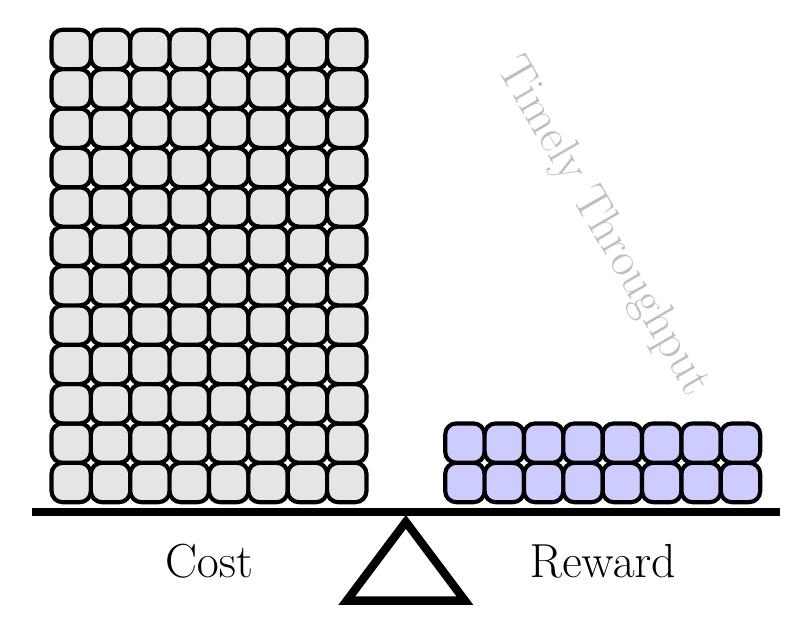
\begin{tikzpicture}
[draw=black, line width=1.5pt, >=stealth',
entry2/.style={rectangle, rounded corners, draw, fill=blue!20, inner sep=0pt, minimum size=5mm},
entry/.style={rectangle, rounded corners, draw, fill=gray!20, inner sep=0pt, minimum size=5mm}]

\node[entry] (m00) at (0,0) {};
\node[entry] (m01) at (0,0.5) {};
\node[entry] (m02) at (0,1) {};
\node[entry] (m03) at (0,1.5) {};
\node[entry] (m04) at (0,2) {};
\node[entry] (m05) at (0,2.5) {};
\node[entry] (m06) at (0,3) {};
\node[entry] (m07) at (0,3.5) {};
\node[entry] (m08) at (0,4) {};
\node[entry] (m09) at (0,4.5) {};
\node[entry] (m010) at (0,5) {};
\node[entry] (m011) at (0,5.5) {};

\node[entry] (m10) at (0.5,0) {};
\node[entry] (m11) at (0.5,0.5) {};
\node[entry] (m12) at (0.5,1) {};
\node[entry] (m13) at (0.5,1.5) {};
\node[entry] (m14) at (0.5,2) {};
\node[entry] (m15) at (0.5,2.5) {};
\node[entry] (m16) at (0.5,3) {};
\node[entry] (m17) at (0.5,3.5) {};
\node[entry] (m18) at (0.5,4) {};
\node[entry] (m19) at (0.5,4.5) {};
\node[entry] (m110) at (0.5,5) {};
\node[entry] (m111) at (0.5,5.5) {};

\node[entry] (m20) at (1,0) {};
\node[entry] (m21) at (1,0.5) {};
\node[entry] (m22) at (1,1) {};
\node[entry] (m23) at (1,1.5) {};
\node[entry] (m24) at (1,2) {};
\node[entry] (m25) at (1,2.5) {};
\node[entry] (m26) at (1,3) {};
\node[entry] (m27) at (1,3.5) {};
\node[entry] (m28) at (1,4) {};
\node[entry] (m29) at (1,4.5) {};
\node[entry] (m210) at (1,5) {};
\node[entry] (m211) at (1,5.5) {};

\node[entry] (m30) at (1.5,0) {};
\node[entry] (m31) at (1.5,0.5) {};
\node[entry] (m32) at (1.5,1) {};
\node[entry] (m33) at (1.5,1.5) {};
\node[entry] (m34) at (1.5,2) {};
\node[entry] (m35) at (1.5,2.5) {};
\node[entry] (m36) at (1.5,3) {};
\node[entry] (m37) at (1.5,3.5) {};
\node[entry] (m38) at (1.5,4) {};
\node[entry] (m39) at (1.5,4.5) {};
\node[entry] (m310) at (1.5,5) {};
\node[entry] (m311) at (1.5,5.5) {};

\node[entry] (m40) at (2,0) {};
\node[entry] (m41) at (2,0.5) {};
\node[entry] (m42) at (2,1) {};
\node[entry] (m43) at (2,1.5) {};
\node[entry] (m44) at (2,2) {};
\node[entry] (m45) at (2,2.5) {};
\node[entry] (m46) at (2,3) {};
\node[entry] (m47) at (2,3.5) {};
\node[entry] (m48) at (2,4) {};
\node[entry] (m49) at (2,4.5) {};
\node[entry] (m410) at (2,5) {};
\node[entry] (m411) at (2,5.5) {};

\node[entry] (m50) at (2.5,0) {};
\node[entry] (m51) at (2.5,0.5) {};
\node[entry] (m52) at (2.5,1) {};
\node[entry] (m53) at (2.5,1.5) {};
\node[entry] (m54) at (2.5,2) {};
\node[entry] (m55) at (2.5,2.5) {};
\node[entry] (m56) at (2.5,3) {};
\node[entry] (m57) at (2.5,3.5) {};
\node[entry] (m58) at (2.5,4) {};
\node[entry] (m59) at (2.5,4.5) {};
\node[entry] (m510) at (2.5,5) {};
\node[entry] (m511) at (2.5,5.5) {};

\node[entry] (m60) at (3,0) {};
\node[entry] (m61) at (3,0.5) {};
\node[entry] (m62) at (3,1) {};
\node[entry] (m63) at (3,1.5) {};
\node[entry] (m64) at (3,2) {};
\node[entry] (m65) at (3,2.5) {};
\node[entry] (m66) at (3,3) {};
\node[entry] (m67) at (3,3.5) {};
\node[entry] (m68) at (3,4) {};
\node[entry] (m69) at (3,4.5) {};
\node[entry] (m610) at (3,5) {};
\node[entry] (m611) at (3,5.5) {};

\node[entry] (m70) at (3.5,0) {};
\node[entry] (m71) at (3.5,0.5) {};
\node[entry] (m72) at (3.5,1) {};
\node[entry] (m73) at (3.5,1.5) {};
\node[entry] (m74) at (3.5,2) {};
\node[entry] (m75) at (3.5,2.5) {};
\node[entry] (m76) at (3.5,3) {};
\node[entry] (m77) at (3.5,3.5) {};
\node[entry] (m78) at (3.5,4) {};
\node[entry] (m79) at (3.5,4.5) {};
\node[entry] (m710) at (3.5,5) {};
\node[entry] (m711) at (3.5,5.5) {};

\node[entry2] (r00) at (5,0) {};
\node[entry2] (r01) at (5,0.5) {};

\node[entry2] (r10) at (5.5,0) {};
\node[entry2] (r11) at (5.5,0.5) {};

\node[entry2] (r20) at (6,0) {};
\node[entry2] (r21) at (6,0.5) {};

\node[entry2] (r30) at (6.5,0) {};
\node[entry2] (r31) at (6.5,0.5) {};

\node[entry2] (r40) at (7,0) {};
\node[entry2] (r41) at (7,0.5) {};

\node[entry2] (r50) at (7.5,0) {};
\node[entry2] (r51) at (7.5,0.5) {};

\node[entry2] (r60) at (8,0) {};
\node[entry2] (r61) at (8,0.5) {};

\node[entry2] (r70) at (8.5,0) {};
\node[entry2] (r71) at (8.5,0.5) {};

\draw[line width=3pt] (-0.5,-0.375) -- (9,-0.375);
\draw[line width=3pt] (3.5,-1.5) -- (4.25,-0.5) -- (5,-1.5) -- (3.5,-1.5) -- (4.25,-0.5);

\node (reward) at (1.75,-1) {\LARGE Cost};
\node (cost) at (6.75,-1) {\LARGE Reward};
\node[rotate=-60] (info) at (6.75,3.25) {\LARGE \textcolor{lightgray}{Timely Throughput}};
\end{tikzpicture}
}
  \end{center}
\end{columns}
\end{frame}


\begin{frame}
\frametitle{Revival of Uncoordinated Access}
\begin{block}{A New Reality}
  \begin{itemize}
  \item Must address sporadic nature of machine-driven communications
  \item Transfer of small payloads without ability to amortize cost of acquiring channel and buffer states over long connections
  \item Preclude use of opportunistic scheduling
  \item Evinced by departure from scheduling-based solutions
% and quest for alternate paradigms
  \end{itemize}
\end{block}
\begin{block}{Communication and Identity}
  When number of devices is massive, with only subset of them active, problem of allocating resources (e.g., codebook, subcarriers, signature sequences) to every user as to manage interference becomes very complex
\end{block}
\begin{center}
\begin{tikzpicture}
\shade[draw=none,
left color={rgb:red,1;green,2;blue,3},
right color=frametitle.fg,
shading angle=60,
rounded corners,
blur shadow={shadow blur steps=5}] (-4.25,-0.625) rectangle (4.25,0.625);
\shade[fill=white, fill opacity=0.1] (-4.25,-0.625) rectangle (4.25,0.625);
\node at (0,0) {\textcolor{white}{\Large \textbf{Uncoordinated, Unsourced MAC}}};
\end{tikzpicture}
\end{center}
\end{frame}


\begin{frame}
\frametitle{Uncoordinated Multiple Access Channel (MAC)}
\begin{center}
\scalebox{0.75}{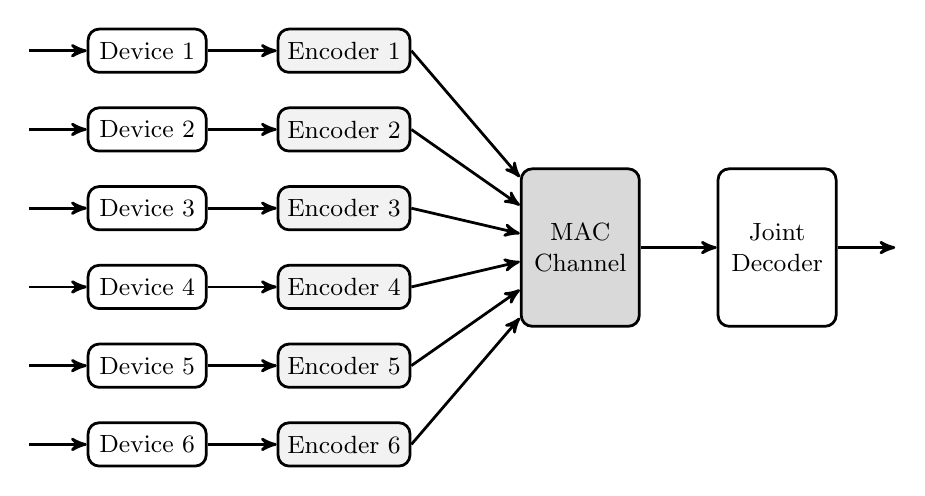
\begin{tikzpicture}
  [
  font=\small, draw=black, >=stealth', line width=1pt,
  channel/.style={rectangle, minimum height=20mm, minimum width=15mm, draw=black, fill=gray!30, rounded corners},
  encoder/.style={rectangle, minimum height=5.5mm, minimum width=15mm, draw=black, fill=gray!10, rounded corners},
  decoder/.style={rectangle, minimum height=20mm, minimum width=15mm, draw=black, rounded corners},
  message/.style={rectangle, minimum height=5.5mm, minimum width=15mm, draw=black, rounded corners}
  ]

\foreach \e in {1,2,3,4,5,6} {
  \node[encoder] (e\e) at (2.5,0.5-\e) {Encoder~${\e}$};
}

\foreach \m in {1,2,3,4,5,6} {
  \node[message] (m\m) at (0.0,0.5-\m) {Device~${\m}$}
  edge[->] (e\m);
  \draw[<-] (m\m) -- (-1.5,0.5-\m);
}
  
\node[channel,align=center] (channel) at (5.5,-3) {MAC\\Channel};
\node[decoder,align=center] (decoder) at (8,-3) {Joint\\Decoder};
\draw[->] (channel) -- (decoder);

\draw[->] (decoder.east) -- (9.5,-3);

\draw[->] (e1.east) -- (channel);
\draw[->] (e2.east) -- (channel);
\draw[->] (e3.east) -- (channel);
\draw[->] (e4.east) -- (channel);
\draw[->] (e5.east) -- (channel);
\draw[->] (e6.east) -- (channel);

\end{tikzpicture}
}
\end{center}
\begin{block}{LoRa-Inspired Parameters}
  \begin{itemize}
  \item $K$ active users out of $K_{\mathrm{tot}}$ total users, $K\in[25:300]$
  \item Each user has $B$-bit message, $B$ is small $\approx 100$
  \item $N$ channel uses available, $N \approx 30,000$
  \end{itemize}
\end{block}
\myfootnote{\tiny
M. Berioli, G. Cocco, G. Liva and A. Munari, \emph{Modern Random Access Protocols}. Foundations and Trends in Networking, 2016}
\myfootnote{\tiny
F. Clazzer, A. Munari, G. Liva, F. Lazaro, C. Stefanovic, P. Popovski, \emph{From 5G to 6G: Has the Time for Modern Random Access Come?}, arXiv 2019}
\end{frame}


\begin{frame}
\frametitle{Uncoordinated MAC Frame Structure}
\begin{itemize}
\item $K$ active devices out of many, many devices
\item Framework of gathering channel and queue states does not apply
\end{itemize}
\begin{center}
  \scalebox{0.8}{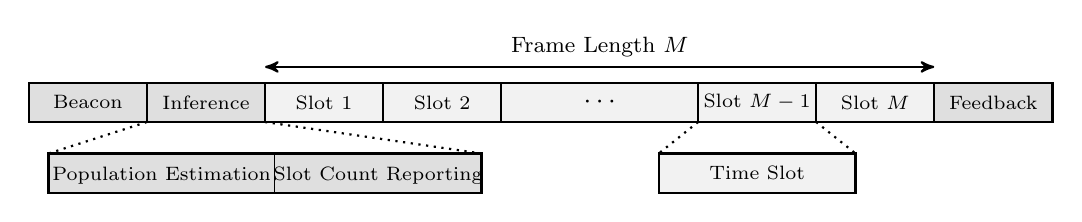
\begin{tikzpicture}[>=stealth', thick]

% --------
\draw [fill=gray!10] (0,0) rectangle (13,0.5);
\draw [<->] (3,0.7) -- node[above]{\footnotesize Frame Length $M$} (11.5,0.7);

\draw [fill=gray!25] (0,0) rectangle (1.5,0.5);
\node at (0.75,0.25) {\scriptsize Beacon};

\draw [fill=gray!25] (1.5,0) rectangle (3,0.5);
\node at (2.25,0.25) {\scriptsize Inference};

\draw (3,0) -- (3,0.5);
\draw (4.5,0) -- (4.5,0.5);
\draw (6,0) -- (6,0.5);
\draw (8.5,0) -- (8.5,0.5);
\draw (10,0) -- (10,0.5);
\draw (11.5,0) -- (11.5,0.5);

\node at (3.75,0.25) {\scriptsize Slot~$1$};
\node at (5.25,0.25) {\scriptsize Slot~$2$};
\node at (7.25,0.25) {$\cdots$};
\node at (9.25,0.25) {\scriptsize Slot~$M - 1$};
\node at (10.75,0.25) {\scriptsize Slot~$M$};

\draw [fill=gray!25] (11.5,0) rectangle (13,0.5);
\node at (12.25,0.25) {\scriptsize Feedback};

% --------
\draw [fill=gray!10] (8,-0.9) rectangle (10.5,-0.4);
\draw [dotted] (8.5,0)--(8,-0.4);
\draw [dotted] (10,0)--(10.5,-0.4);
\node at (9.25,-0.65) {\scriptsize Time Slot};

% --------
\draw [fill=gray!25] (0.25,-0.9) rectangle (5.75,-0.4);
\node at (1.6875,-0.675) {\scriptsize Population Estimation};
\node at (4.4375,-0.675) {\scriptsize Slot Count Reporting};
\draw [dotted] (1.5,0)--(0.25,-0.4);
\draw [dotted] (3,0)--(5.75,-0.4);
\draw[thin] (3.125,-0.4) -- (3.125,-0.9);

\end{tikzpicture} 

}
\end{center}
\begin{itemize}
\item Beacon employed for coarse synchronization
\item Same devices transmit within frame
\item Each device may or may not use slot
\end{itemize}
\myfootnote{\tiny
X. Chen and D. Guo. \emph{Many-access channels: The Gaussian case with random user activities}. ISIT, 2014}
\end{frame}


\begin{frame}
\frametitle{Uncoordinated and Unsourced MAC}
\begin{center}
\scalebox{0.75}{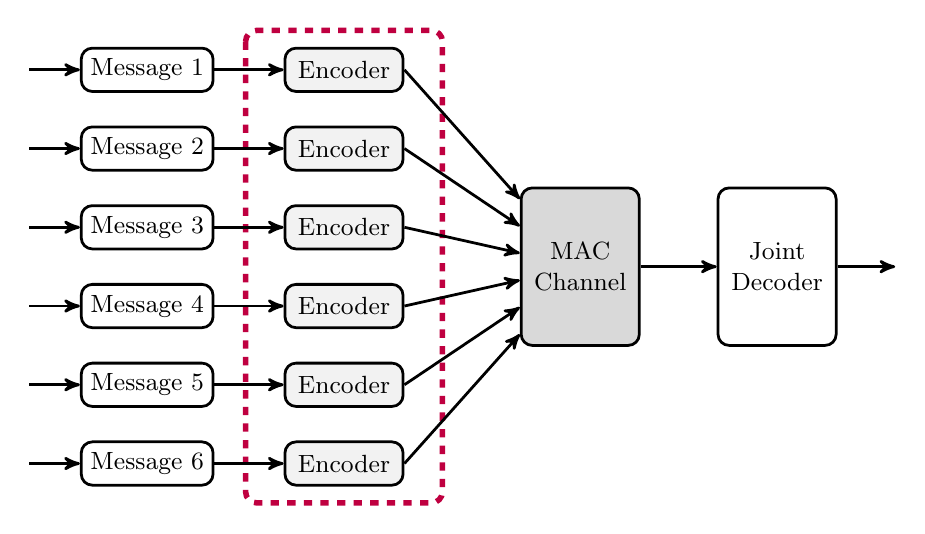
\begin{tikzpicture}
  [
  font=\small, draw=black, >=stealth', line width=1pt,
  channel/.style={rectangle, minimum height=20mm, minimum width=15mm, draw=black, fill=gray!30, rounded corners},
  encoder/.style={rectangle, minimum height=5.5mm, minimum width=15mm, draw=black, fill=gray!10, rounded corners},
  decoder/.style={rectangle, minimum height=20mm, minimum width=15mm, draw=black, rounded corners},
  message/.style={rectangle, minimum height=5.5mm, minimum width=15mm, draw=black, rounded corners}
  ]

\foreach \e in {1,2,3,4,5,6} {
  \node[encoder] (e\e) at (2.5,0.5-\e) {Encoder};
}

\draw[draw=purple, dashed, line width=2.0pt,rounded corners] (1.25, 0) rectangle (3.75, -6);

\foreach \m in {1,2,3,4,5,6} {
  \node[message] (m\m) at (0.0,0.5-\m) {Message~${\m}$}
  edge[->] (e\m);
  \draw[<-] (m\m) -- (-1.5,0.5-\m);
}
  
\node[channel,align=center] (channel) at (5.5,-3) {MAC\\Channel};
\node[decoder,align=center] (decoder) at (8,-3) {Joint\\Decoder};
\draw[->] (channel) -- (decoder);

\draw[->] (decoder.east) -- (9.5,-3);

\draw[->] (e1.east) -- (channel);
\draw[->] (e2.east) -- (channel);
\draw[->] (e3.east) -- (channel);
\draw[->] (e4.east) -- (channel);
\draw[->] (e5.east) -- (channel);
\draw[->] (e6.east) -- (channel);

\end{tikzpicture}
}
\end{center}
\begin{columns}
\column{.53\textwidth}
\begin{block}{Without Personalized Feedback}
  \begin{itemize}
  \item All devices employ same encoder
  \item No explicit knowledge of identities
  \item Need only return unordered list
  \end{itemize}
\end{block}
\column{.45\textwidth}
\begin{block}{Math Model}
  \begin{equation*}
  \textstyle \vec{y}
  = \sum_{i \in \mathbf{S}_{\mathrm{a}}} \vec{x}_i + \vec{n}
  \end{equation*}
  where $\mathbf{x}_i = f(w_i)$ is codeword, only depends on message
\end{block}
\end{columns}
\myfootnote{\tiny
Y. Polyanskiy. \emph{A Perspective on Massive Random-Access}. ISIT, 2017}
\end{frame}

\begin{frame}
\frametitle{Gaussian Random Codes \& Performance Bounds}

\begin{center}
\begin{tikzpicture}
\node[scope fading=south] (image) at (0,0) {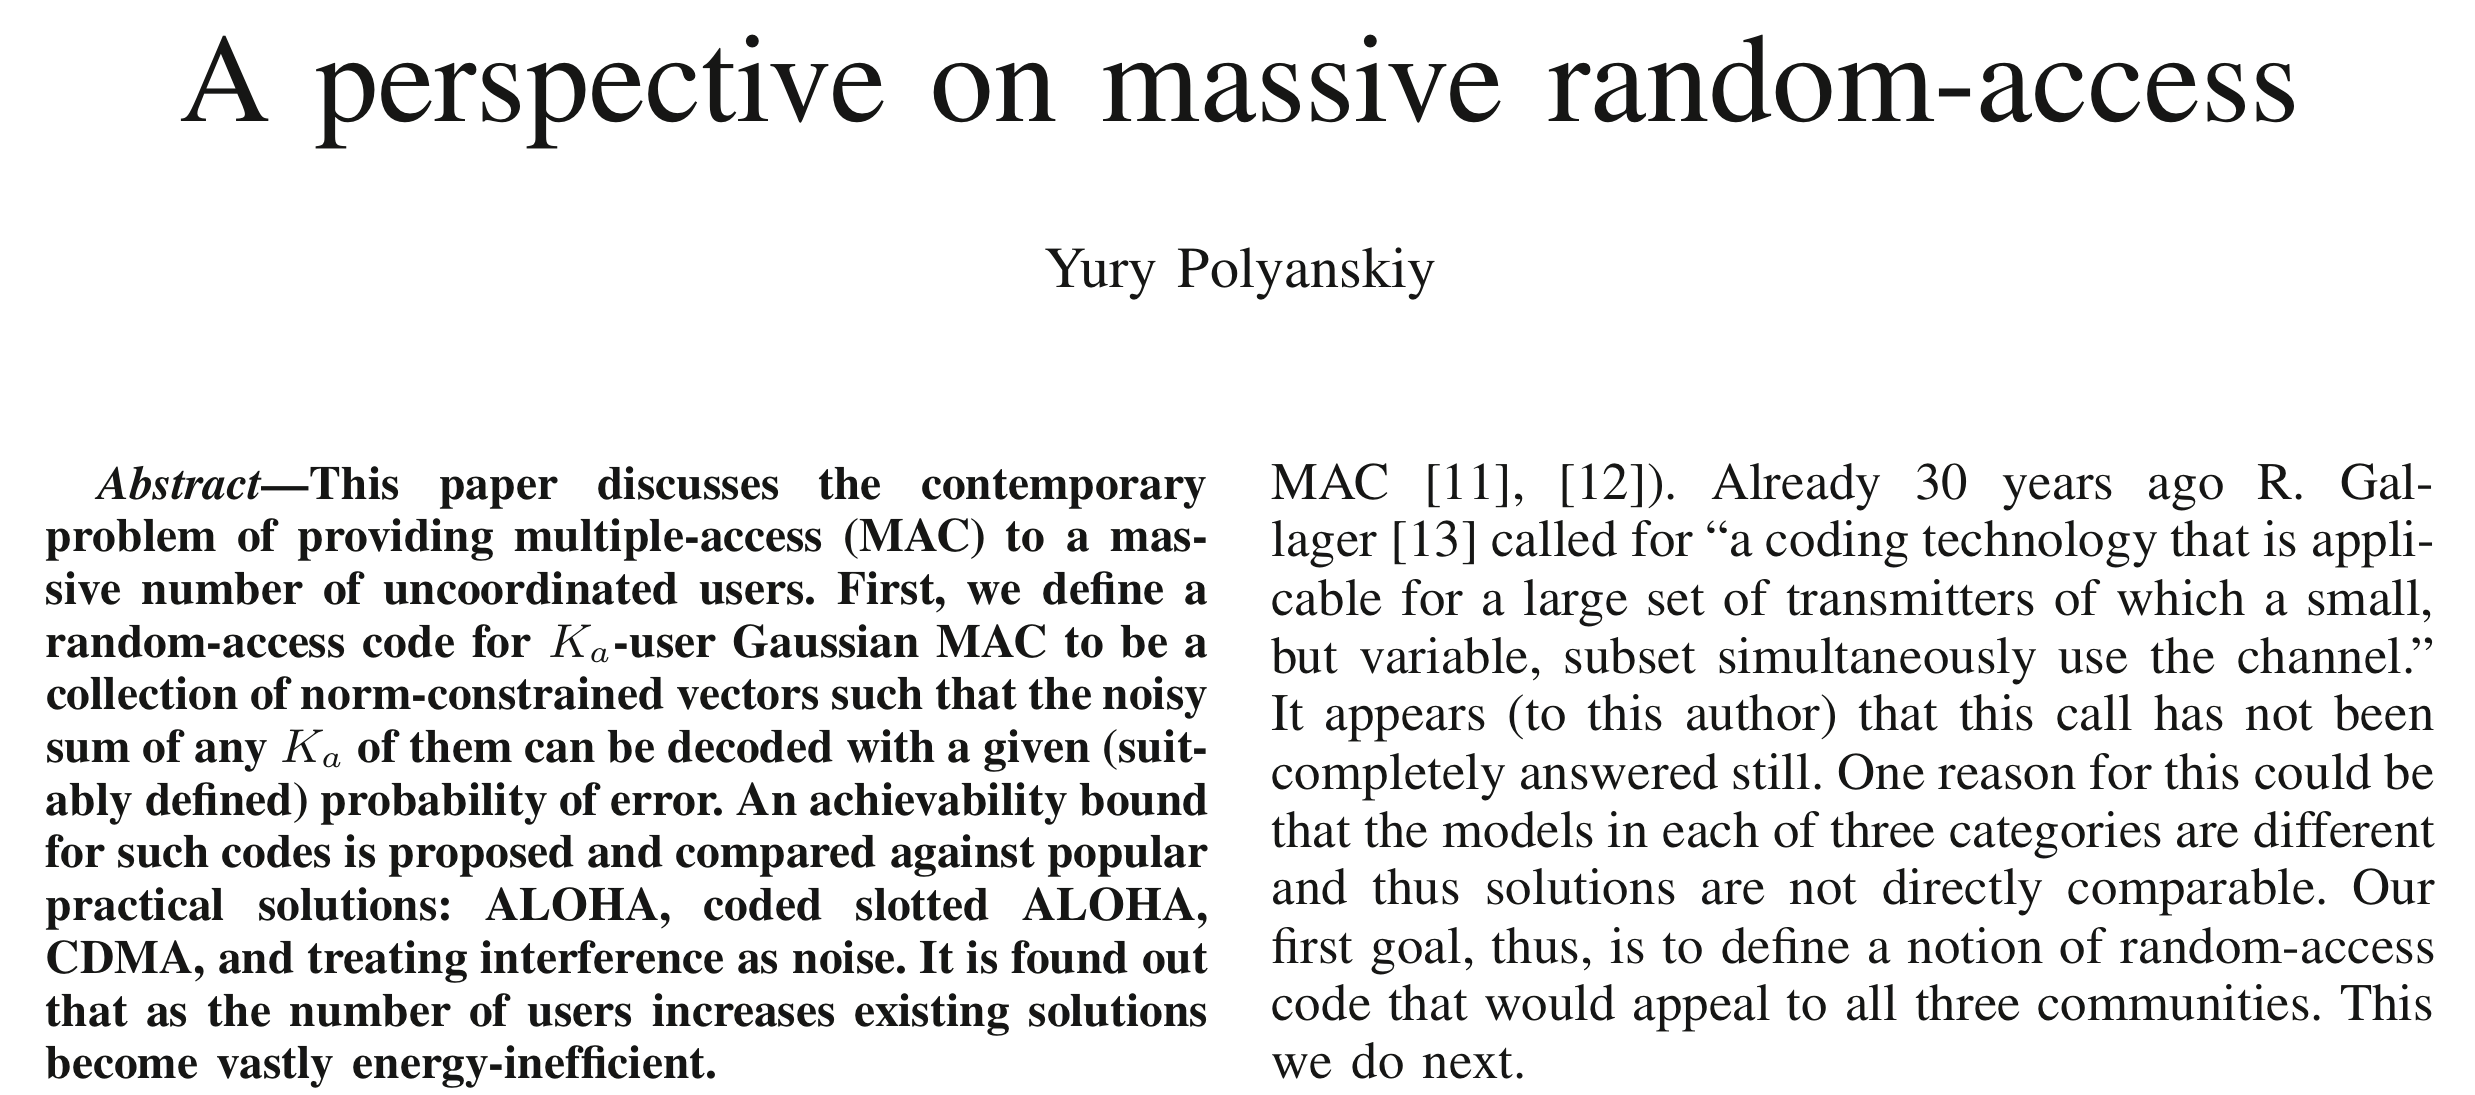
\includegraphics[width=3.5in]{Figures/ISIT2017Polyanskiy.png}};
\end{tikzpicture}
\end{center}

\textbf{Theorem}:
Fix $P' < P$.
There exists an $(M, n, \epsilon)$ random-access code for the $K$-user GMAC satisfying power-constraint $P$ and
\begin{equation*}
\textstyle \epsilon \leq \sum_{t=1}^{K} \frac{t}{K} \min (p_t, q_t) + p_0 ,
\end{equation*}
where constants $p_0$, $p_t$, and $q_t$ are complicated
\myfootnote{\tiny
Y. Polyanskiy. \emph{A Perspective on Massive Random-Access}. ISIT, 2017}
\end{frame}


\begin{frame}
\frametitle{UMAC -- Compressed Sensing Interpretation}
\centerline{\centerline{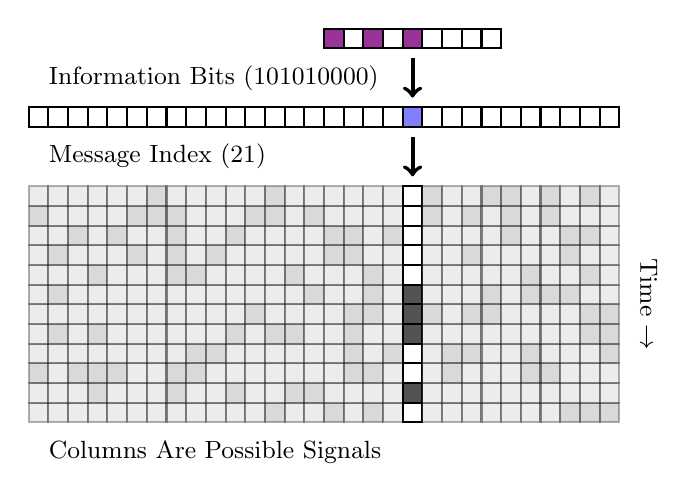
\begin{tikzpicture}
[font=\small, draw=black, line width=0.75pt,
bit0/.style={rectangle, draw, inner sep=0pt, minimum size=2.5mm},
bit1/.style={rectangle, draw, fill=violet!80, inner sep=0pt, minimum size=2.5mm},
entry0/.style={rectangle, draw, opacity=0.3, fill=lightgray, inner sep=0pt, minimum size=2.5mm},
entry1/.style={rectangle, draw, opacity=0.3, fill=gray, inner sep=0pt, minimum size=2.5mm},
entry00/.style={rectangle, draw, fill=white, inner sep=0pt, minimum size=2.5mm},
entry11/.style={rectangle, draw, fill=darkgray!90, inner sep=0pt, minimum size=2.5mm},
symbol0/.style={rectangle, draw, fill=white, inner sep=0pt, minimum size=2.5mm},
symbol1/.style={rectangle, draw, fill=blue!50, inner sep=0pt, minimum size=2.5mm}]

\node[entry0] (m0000) at (0.00,0) {};
\node[entry0] (m0100) at (0.25,0) {};
\node[entry0] (m0200) at (0.50,0) {};
\node[entry0] (m0300) at (0.75,0) {};
\node[entry0] (m0400) at (1.00,0) {};
\node[entry0] (m0500) at (1.25,0) {};
\node[entry0] (m0600) at (1.50,0) {};
\node[entry0] (m0700) at (1.75,0) {};
\node[entry0] (m0800) at (2.00,0) {};
\node[entry0] (m0900) at (2.25,0) {};
\node[entry0] (m1000) at (2.50,0) {};
\node[entry0] (m1100) at (2.75,0) {};
\node[entry1] (m1200) at (3.00,0) {};
\node[entry0] (m1300) at (3.25,0) {};
\node[entry0] (m1400) at (3.50,0) {};
\node[entry1] (m1500) at (3.75,0) {};
\node[entry0] (m1600) at (4.00,0) {};
\node[entry1] (m1700) at (4.25,0) {};
\node[entry0] (m1800) at (4.50,0) {};
\node[entry00] (m1900) at (4.75,0) {};
\node[entry0] (m2000) at (5.00,0) {};
\node[entry0] (m2100) at (5.25,0) {};
\node[entry0] (m2200) at (5.50,0) {};
\node[entry0] (m2300) at (5.75,0) {};
\node[entry0] (m2400) at (6.00,0) {};
\node[entry0] (m2500) at (6.25,0) {};
\node[entry0] (m2600) at (6.50,0) {};
\node[entry1] (m2700) at (6.75,0) {};
\node[entry1] (m2800) at (7.00,0) {};
\node[entry1] (m2900) at (7.25,0) {};

\node[entry0] (m0001) at (0.00,0.25) {};
\node[entry0] (m0101) at (0.25,0.25) {};
\node[entry0] (m0201) at (0.50,0.25) {};
\node[entry1] (m0301) at (0.75,0.25) {};
\node[entry0] (m0401) at (1.00,0.25) {};
\node[entry0] (m0501) at (1.25,0.25) {};
\node[entry0] (m0601) at (1.50,0.25) {};
\node[entry1] (m0701) at (1.75,0.25) {};
\node[entry0] (m0801) at (2.00,0.25) {};
\node[entry0] (m0901) at (2.25,0.25) {};
\node[entry1] (m1001) at (2.50,0.25) {};
\node[entry0] (m1101) at (2.75,0.25) {};
\node[entry0] (m1201) at (3.00,0.25) {};
\node[entry1] (m1301) at (3.25,0.25) {};
\node[entry1] (m1401) at (3.50,0.25) {};
\node[entry0] (m1501) at (3.75,0.25) {};
\node[entry0] (m1601) at (4.00,0.25) {};
\node[entry0] (m1701) at (4.25,0.25) {};
\node[entry0] (m1801) at (4.50,0.25) {};
\node[entry11] (m1901) at (4.75,0.25) {};
\node[entry0] (m2001) at (5.00,0.25) {};
\node[entry0] (m2101) at (5.25,0.25) {};
\node[entry0] (m2201) at (5.50,0.25) {};
\node[entry0] (m2301) at (5.75,0.25) {};
\node[entry0] (m2401) at (6.00,0.25) {};
\node[entry0] (m2501) at (6.25,0.25) {};
\node[entry0] (m2601) at (6.50,0.25) {};
\node[entry0] (m2701) at (6.75,0.25) {};
\node[entry0] (m2801) at (7.00,0.25) {};
\node[entry0] (m2901) at (7.25,0.25) {};

\node[entry1] (m0002) at (0.00,0.50) {};
\node[entry0] (m0102) at (0.25,0.50) {};
\node[entry1] (m0202) at (0.50,0.50) {};
\node[entry1] (m0302) at (0.75,0.50) {};
\node[entry1] (m0402) at (1.00,0.50) {};
\node[entry0] (m0502) at (1.25,0.50) {};
\node[entry0] (m0602) at (1.50,0.50) {};
\node[entry1] (m0702) at (1.75,0.50) {};
\node[entry1] (m0802) at (2.00,0.50) {};
\node[entry0] (m0902) at (2.25,0.50) {};
\node[entry0] (m1002) at (2.50,0.50) {};
\node[entry0] (m1102) at (2.75,0.50) {};
\node[entry0] (m1202) at (3.00,0.50) {};
\node[entry0] (m1302) at (3.25,0.50) {};
\node[entry0] (m1402) at (3.50,0.50) {};
\node[entry0] (m1502) at (3.75,0.50) {};
\node[entry1] (m1602) at (4.00,0.50) {};
\node[entry1] (m1702) at (4.25,0.50) {};
\node[entry0] (m1802) at (4.50,0.50) {};
\node[entry00] (m1902) at (4.75,0.50) {};
\node[entry0] (m2002) at (5.00,0.50) {};
\node[entry1] (m2102) at (5.25,0.50) {};
\node[entry0] (m2202) at (5.50,0.50) {};
\node[entry0] (m2302) at (5.75,0.50) {};
\node[entry0] (m2402) at (6.00,0.50) {};
\node[entry1] (m2502) at (6.25,0.50) {};
\node[entry1] (m2602) at (6.50,0.50) {};
\node[entry0] (m2702) at (6.75,0.50) {};
\node[entry0] (m2802) at (7.00,0.50) {};
\node[entry0] (m2902) at (7.25,0.50) {};

\node[entry0] (m0003) at (0.00,0.75) {};
\node[entry0] (m0103) at (0.25,0.75) {};
\node[entry0] (m0203) at (0.50,0.75) {};
\node[entry0] (m0303) at (0.75,0.75) {};
\node[entry0] (m0403) at (1.00,0.75) {};
\node[entry0] (m0503) at (1.25,0.75) {};
\node[entry0] (m0603) at (1.50,0.75) {};
\node[entry0] (m0703) at (1.75,0.75) {};
\node[entry1] (m0803) at (2.00,0.75) {};
\node[entry1] (m0903) at (2.25,0.75) {};
\node[entry0] (m1003) at (2.50,0.75) {};
\node[entry0] (m1103) at (2.75,0.75) {};
\node[entry0] (m1203) at (3.00,0.75) {};
\node[entry0] (m1303) at (3.25,0.75) {};
\node[entry0] (m1403) at (3.50,0.75) {};
\node[entry0] (m1503) at (3.75,0.75) {};
\node[entry1] (m1603) at (4.00,0.75) {};
\node[entry0] (m1703) at (4.25,0.75) {};
\node[entry1] (m1803) at (4.50,0.75) {};
\node[entry00] (m1903) at (4.75,0.75) {};
\node[entry0] (m2003) at (5.00,0.75) {};
\node[entry1] (m2103) at (5.25,0.75) {};
\node[entry1] (m2203) at (5.50,0.75) {};
\node[entry0] (m2303) at (5.75,0.75) {};
\node[entry0] (m2403) at (6.00,0.75) {};
\node[entry1] (m2503) at (6.25,0.75) {};
\node[entry0] (m2603) at (6.50,0.75) {};
\node[entry0] (m2703) at (6.75,0.75) {};
\node[entry0] (m2803) at (7.00,0.75) {};
\node[entry1] (m2903) at (7.25,0.75) {};

\node[entry0] (m0004) at (0.00,1.00) {};
\node[entry1] (m0104) at (0.25,1.00) {};
\node[entry0] (m0204) at (0.50,1.00) {};
\node[entry1] (m0304) at (0.75,1.00) {};
\node[entry0] (m0404) at (1.00,1.00) {};
\node[entry0] (m0504) at (1.25,1.00) {};
\node[entry0] (m0604) at (1.50,1.00) {};
\node[entry0] (m0704) at (1.75,1.00) {};
\node[entry0] (m0804) at (2.00,1.00) {};
\node[entry0] (m0904) at (2.25,1.00) {};
\node[entry1] (m1004) at (2.50,1.00) {};
\node[entry0] (m1104) at (2.75,1.00) {};
\node[entry1] (m1204) at (3.00,1.00) {};
\node[entry1] (m1304) at (3.25,1.00) {};
\node[entry0] (m1404) at (3.50,1.00) {};
\node[entry0] (m1504) at (3.75,1.00) {};
\node[entry1] (m1604) at (4.00,1.00) {};
\node[entry0] (m1704) at (4.25,1.00) {};
\node[entry0] (m1804) at (4.50,1.00) {};
\node[entry11] (m1904) at (4.75,1.00) {};
\node[entry0] (m2004) at (5.00,1.00) {};
\node[entry0] (m2104) at (5.25,1.00) {};
\node[entry0] (m2204) at (5.50,1.00) {};
\node[entry0] (m2304) at (5.75,1.00) {};
\node[entry0] (m2404) at (6.00,1.00) {};
\node[entry0] (m2504) at (6.25,1.00) {};
\node[entry0] (m2604) at (6.50,1.00) {};
\node[entry0] (m2704) at (6.75,1.00) {};
\node[entry1] (m2804) at (7.00,1.00) {};
\node[entry1] (m2904) at (7.25,1.00) {};

\node[entry0] (m0005) at (0.00,1.25) {};
\node[entry0] (m0105) at (0.25,1.25) {};
\node[entry0] (m0205) at (0.50,1.25) {};
\node[entry0] (m0305) at (0.75,1.25) {};
\node[entry0] (m0405) at (1.00,1.25) {};
\node[entry0] (m0505) at (1.25,1.25) {};
\node[entry0] (m0605) at (1.50,1.25) {};
\node[entry0] (m0705) at (1.75,1.25) {};
\node[entry0] (m0805) at (2.00,1.25) {};
\node[entry0] (m0905) at (2.25,1.25) {};
\node[entry0] (m1005) at (2.50,1.25) {};
\node[entry1] (m1105) at (2.75,1.25) {};
\node[entry0] (m1205) at (3.00,1.25) {};
\node[entry0] (m1305) at (3.25,1.25) {};
\node[entry0] (m1405) at (3.50,1.25) {};
\node[entry0] (m1505) at (3.75,1.25) {};
\node[entry1] (m1605) at (4.00,1.25) {};
\node[entry1] (m1705) at (4.25,1.25) {};
\node[entry0] (m1805) at (4.50,1.25) {};
\node[entry11] (m1905) at (4.75,1.25) {};
\node[entry1] (m2005) at (5.00,1.25) {};
\node[entry0] (m2105) at (5.25,1.25) {};
\node[entry1] (m2205) at (5.50,1.25) {};
\node[entry1] (m2305) at (5.75,1.25) {};
\node[entry0] (m2405) at (6.00,1.25) {};
\node[entry0] (m2505) at (6.25,1.25) {};
\node[entry0] (m2605) at (6.50,1.25) {};
\node[entry0] (m2705) at (6.75,1.25) {};
\node[entry1] (m2805) at (7.00,1.25) {};
\node[entry1] (m2905) at (7.25,1.25) {};

\node[entry0] (m0006) at (0.00,1.50) {};
\node[entry1] (m0106) at (0.25,1.50) {};
\node[entry0] (m0206) at (0.50,1.50) {};
\node[entry0] (m0306) at (0.75,1.50) {};
\node[entry0] (m0406) at (1.00,1.50) {};
\node[entry0] (m0506) at (1.25,1.50) {};
\node[entry0] (m0606) at (1.50,1.50) {};
\node[entry0] (m0706) at (1.75,1.50) {};
\node[entry0] (m0806) at (2.00,1.50) {};
\node[entry0] (m0906) at (2.25,1.50) {};
\node[entry0] (m1006) at (2.50,1.50) {};
\node[entry0] (m1106) at (2.75,1.50) {};
\node[entry0] (m1206) at (3.00,1.50) {};
\node[entry0] (m1306) at (3.25,1.50) {};
\node[entry1] (m1406) at (3.50,1.50) {};
\node[entry0] (m1506) at (3.75,1.50) {};
\node[entry0] (m1606) at (4.00,1.50) {};
\node[entry1] (m1706) at (4.25,1.50) {};
\node[entry0] (m1806) at (4.50,1.50) {};
\node[entry11] (m1906) at (4.75,1.50) {};
\node[entry0] (m2006) at (5.00,1.50) {};
\node[entry0] (m2106) at (5.25,1.50) {};
\node[entry0] (m2206) at (5.50,1.50) {};
\node[entry1] (m2306) at (5.75,1.50) {};
\node[entry0] (m2406) at (6.00,1.50) {};
\node[entry1] (m2506) at (6.25,1.50) {};
\node[entry1] (m2606) at (6.50,1.50) {};
\node[entry1] (m2706) at (6.75,1.50) {};
\node[entry0] (m2806) at (7.00,1.50) {};
\node[entry0] (m2906) at (7.25,1.50) {};

\node[entry0] (m0007) at (0.00,1.75) {};
\node[entry0] (m0107) at (0.25,1.75) {};
\node[entry0] (m0207) at (0.50,1.75) {};
\node[entry1] (m0307) at (0.75,1.75) {};
\node[entry0] (m0407) at (1.00,1.75) {};
\node[entry0] (m0507) at (1.25,1.75) {};
\node[entry0] (m0607) at (1.50,1.75) {};
\node[entry1] (m0707) at (1.75,1.75) {};
\node[entry1] (m0807) at (2.00,1.75) {};
\node[entry0] (m0907) at (2.25,1.75) {};
\node[entry0] (m1007) at (2.50,1.75) {};
\node[entry0] (m1107) at (2.75,1.75) {};
\node[entry0] (m1207) at (3.00,1.75) {};
\node[entry1] (m1307) at (3.25,1.75) {};
\node[entry0] (m1407) at (3.50,1.75) {};
\node[entry0] (m1507) at (3.75,1.75) {};
\node[entry0] (m1607) at (4.00,1.75) {};
\node[entry1] (m1707) at (4.25,1.75) {};
\node[entry0] (m1807) at (4.50,1.75) {};
\node[entry00] (m1907) at (4.75,1.75) {};
\node[entry0] (m2007) at (5.00,1.75) {};
\node[entry0] (m2107) at (5.25,1.75) {};
\node[entry0] (m2207) at (5.50,1.75) {};
\node[entry0] (m2307) at (5.75,1.75) {};
\node[entry0] (m2407) at (6.00,1.75) {};
\node[entry1] (m2507) at (6.25,1.75) {};
\node[entry0] (m2607) at (6.50,1.75) {};
\node[entry0] (m2707) at (6.75,1.75) {};
\node[entry1] (m2807) at (7.00,1.75) {};
\node[entry0] (m2907) at (7.25,1.75) {};

\node[entry0] (m0008) at (0.00,2.00) {};
\node[entry1] (m0108) at (0.25,2.00) {};
\node[entry0] (m0208) at (0.50,2.00) {};
\node[entry0] (m0308) at (0.75,2.00) {};
\node[entry0] (m0408) at (1.00,2.00) {};
\node[entry1] (m0508) at (1.25,2.00) {};
\node[entry0] (m0608) at (1.50,2.00) {};
\node[entry1] (m0708) at (1.75,2.00) {};
\node[entry0] (m0808) at (2.00,2.00) {};
\node[entry1] (m0908) at (2.25,2.00) {};
\node[entry0] (m1008) at (2.50,2.00) {};
\node[entry0] (m1108) at (2.75,2.00) {};
\node[entry0] (m1208) at (3.00,2.00) {};
\node[entry0] (m1308) at (3.25,2.00) {};
\node[entry0] (m1408) at (3.50,2.00) {};
\node[entry1] (m1508) at (3.75,2.00) {};
\node[entry1] (m1608) at (4.00,2.00) {};
\node[entry0] (m1708) at (4.25,2.00) {};
\node[entry0] (m1808) at (4.50,2.00) {};
\node[entry00] (m1908) at (4.75,2.00) {};
\node[entry0] (m2008) at (5.00,2.00) {};
\node[entry0] (m2108) at (5.25,2.00) {};
\node[entry1] (m2208) at (5.50,2.00) {};
\node[entry0] (m2308) at (5.75,2.00) {};
\node[entry0] (m2408) at (6.00,2.00) {};
\node[entry0] (m2508) at (6.25,2.00) {};
\node[entry0] (m2608) at (6.50,2.00) {};
\node[entry1] (m2708) at (6.75,2.00) {};
\node[entry0] (m2808) at (7.00,2.00) {};
\node[entry0] (m2908) at (7.25,2.00) {};

\node[entry0] (m0009) at (0.00,2.25) {};
\node[entry0] (m0109) at (0.25,2.25) {};
\node[entry1] (m0209) at (0.50,2.25) {};
\node[entry0] (m0309) at (0.75,2.25) {};
\node[entry1] (m0409) at (1.00,2.25) {};
\node[entry0] (m0509) at (1.25,2.25) {};
\node[entry0] (m0609) at (1.50,2.25) {};
\node[entry1] (m0709) at (1.75,2.25) {};
\node[entry0] (m0809) at (2.00,2.25) {};
\node[entry0] (m0909) at (2.25,2.25) {};
\node[entry1] (m1009) at (2.50,2.25) {};
\node[entry0] (m1109) at (2.75,2.25) {};
\node[entry0] (m1209) at (3.00,2.25) {};
\node[entry0] (m1309) at (3.25,2.25) {};
\node[entry0] (m1409) at (3.50,2.25) {};
\node[entry1] (m1509) at (3.75,2.25) {};
\node[entry1] (m1609) at (4.00,2.25) {};
\node[entry0] (m1709) at (4.25,2.25) {};
\node[entry1] (m1809) at (4.50,2.25) {};
\node[entry00] (m1909) at (4.75,2.25) {};
\node[entry0] (m2009) at (5.00,2.25) {};
\node[entry0] (m2109) at (5.25,2.25) {};
\node[entry0] (m2209) at (5.50,2.25) {};
\node[entry0] (m2309) at (5.75,2.25) {};
\node[entry1] (m2409) at (6.00,2.25) {};
\node[entry0] (m2509) at (6.25,2.25) {};
\node[entry0] (m2609) at (6.50,2.25) {};
\node[entry1] (m2709) at (6.75,2.25) {};
\node[entry1] (m2809) at (7.00,2.25) {};
\node[entry0] (m2909) at (7.25,2.25) {};

\node[entry1] (m0010) at (0.00,2.50) {};
\node[entry0] (m0110) at (0.25,2.50) {};
\node[entry0] (m0210) at (0.50,2.50) {};
\node[entry0] (m0310) at (0.75,2.50) {};
\node[entry0] (m0410) at (1.00,2.50) {};
\node[entry1] (m0510) at (1.25,2.50) {};
\node[entry1] (m0610) at (1.50,2.50) {};
\node[entry1] (m0710) at (1.75,2.50) {};
\node[entry0] (m0810) at (2.00,2.50) {};
\node[entry0] (m0910) at (2.25,2.50) {};
\node[entry0] (m1010) at (2.50,2.50) {};
\node[entry1] (m1110) at (2.75,2.50) {};
\node[entry1] (m1210) at (3.00,2.50) {};
\node[entry0] (m1310) at (3.25,2.50) {};
\node[entry1] (m1410) at (3.50,2.50) {};
\node[entry0] (m1510) at (3.75,2.50) {};
\node[entry0] (m1610) at (4.00,2.50) {};
\node[entry0] (m1710) at (4.25,2.50) {};
\node[entry0] (m1810) at (4.50,2.50) {};
\node[entry00] (m1910) at (4.75,2.50) {};
\node[entry1] (m2010) at (5.00,2.50) {};
\node[entry0] (m2110) at (5.25,2.50) {};
\node[entry1] (m2210) at (5.50,2.50) {};
\node[entry0] (m2310) at (5.75,2.50) {};
\node[entry1] (m2410) at (6.00,2.50) {};
\node[entry0] (m2510) at (6.25,2.50) {};
\node[entry1] (m2610) at (6.50,2.50) {};
\node[entry0] (m2710) at (6.75,2.50) {};
\node[entry0] (m2810) at (7.00,2.50) {};
\node[entry0] (m2910) at (7.25,2.50) {};

\node[entry0] (m0011) at (0.00,2.75) {};
\node[entry0] (m0111) at (0.25,2.75) {};
\node[entry0] (m0211) at (0.50,2.75) {};
\node[entry0] (m0311) at (0.75,2.75) {};
\node[entry0] (m0411) at (1.00,2.75) {};
\node[entry0] (m0511) at (1.25,2.75) {};
\node[entry1] (m0611) at (1.50,2.75) {};
\node[entry0] (m0711) at (1.75,2.75) {};
\node[entry0] (m0811) at (2.00,2.75) {};
\node[entry0] (m0911) at (2.25,2.75) {};
\node[entry0] (m1011) at (2.50,2.75) {};
\node[entry0] (m1111) at (2.75,2.75) {};
\node[entry1] (m1211) at (3.00,2.75) {};
\node[entry0] (m1311) at (3.25,2.75) {};
\node[entry0] (m1411) at (3.50,2.75) {};
\node[entry0] (m1511) at (3.75,2.75) {};
\node[entry0] (m1611) at (4.00,2.75) {};
\node[entry0] (m1711) at (4.25,2.75) {};
\node[entry0] (m1811) at (4.50,2.75) {};
\node[entry00] (m1911) at (4.75,2.75) {};
\node[entry1] (m2011) at (5.00,2.75) {};
\node[entry0] (m2111) at (5.25,2.75) {};
\node[entry0] (m2211) at (5.50,2.75) {};
\node[entry1] (m2311) at (5.75,2.75) {};
\node[entry1] (m2411) at (6.00,2.75) {};
\node[entry0] (m2511) at (6.25,2.75) {};
\node[entry1] (m2611) at (6.50,2.75) {};
\node[entry0] (m2711) at (6.75,2.75) {};
\node[entry1] (m2811) at (7.00,2.75) {};
\node[entry0] (m2911) at (7.25,2.75) {};

\draw[->, line width=1.5pt]  (4.75,3.50) -- (4.75,3.00);

\node[symbol0] (s00) at (0.00,3.75) {};
\node[symbol0] (s01) at (0.25,3.75) {};
\node[symbol0] (s02) at (0.50,3.75) {};
\node[symbol0] (s03) at (0.75,3.75) {};
\node[symbol0] (s04) at (1.00,3.75) {};
\node[symbol0] (s05) at (1.25,3.75) {};
\node[symbol0] (s06) at (1.50,3.75) {};
\node[symbol0] (s07) at (1.75,3.75) {};
\node[symbol0] (s08) at (2.00,3.75) {};
\node[symbol0] (s09) at (2.25,3.75) {};
\node[symbol0] (s10) at (2.50,3.75) {};
\node[symbol0] (s11) at (2.75,3.75) {};
\node[symbol0] (s12) at (3.00,3.75) {};
\node[symbol0] (s13) at (3.25,3.75) {};
\node[symbol0] (s14) at (3.50,3.75) {};
\node[symbol0] (s15) at (3.75,3.75) {};
\node[symbol0] (s16) at (4.00,3.75) {};
\node[symbol0] (s17) at (4.25,3.75) {};
\node[symbol0] (s18) at (4.50,3.75) {};
\node[symbol1] (s19) at (4.75,3.75) {};
\node[symbol0] (s20) at (5.00,3.75) {};
\node[symbol0] (s21) at (5.25,3.75) {};
\node[symbol0] (s22) at (5.50,3.75) {};
\node[symbol0] (s23) at (5.75,3.75) {};
\node[symbol0] (s24) at (6.00,3.75) {};
\node[symbol0] (s25) at (6.25,3.75) {};
\node[symbol0] (s26) at (6.50,3.75) {};
\node[symbol0] (s27) at (6.75,3.75) {};
\node[symbol0] (s28) at (7.00,3.75) {};
\node[symbol0] (s29) at (7.25,3.75) {};

\draw[->, line width=1.5pt]  (4.75,4.50) -- (4.75,4.00);

\node[bit1] (info0) at (3.75,4.75) {};
\node[bit0] (info1) at (4.00,4.75) {};
\node[bit1] (info2) at (4.25,4.75) {};
\node[bit0] (info3) at (4.50,4.75) {};
\node[bit1] (info4) at (4.75,4.75) {};
\node[bit0] (info5) at (5.00,4.75) {};
\node[bit0] (info6) at (5.25,4.75) {};
\node[bit0] (info7) at (5.50,4.75) {};
\node[bit0] (info8) at (5.75,4.75) {};


\node [anchor = west] (infobits) at (0.00,4.25) {Information Bits (101010000)};
\node [anchor = west] (messageindex) at (0.00,3.25) {Message Index (21)};
\node [anchor = west] (signals) at (0.00,-0.50) {Columns Are Possible Signals};
\node[rotate=-90] (time) at (7.75,1.375) {Time $\rightarrow$};
\end{tikzpicture}
}}
\vfill
\begin{itemize}
\item Bit sequence $\underbar{w}_i \in \{ 0,1 \}^B$ converted to index in $[1,2^B]$
\item Stack codewords into $N \times 2^B$ \emph{sensing} matrix
\item Message index determines transmitted codeword
\end{itemize}
\end{frame}


\begin{frame}
\frametitle{UMAC -- Compressed Sensing with Multiple Messages}
\centerline{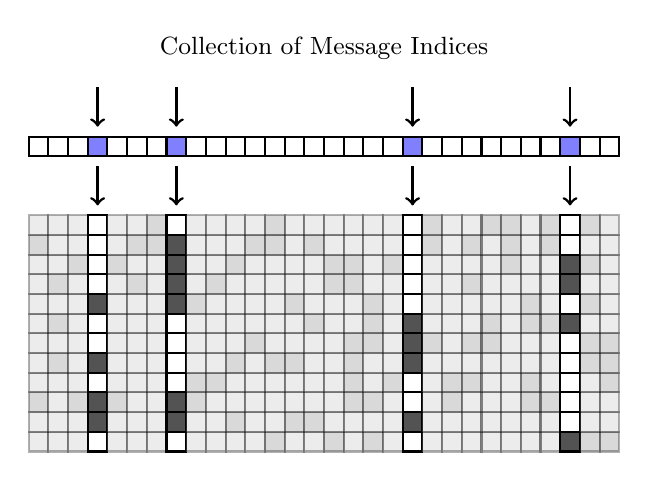
\begin{tikzpicture}
[font=\small, draw=black, line width=0.75pt,
entry0/.style={rectangle, draw, opacity=0.3, fill=lightgray, inner sep=0pt, minimum size=2.5mm},
entry1/.style={rectangle, draw, opacity=0.3, fill=gray, inner sep=0pt, minimum size=2.5mm},
entry00/.style={rectangle, draw, fill=white, inner sep=0pt, minimum size=2.5mm},
entry11/.style={rectangle, draw, fill=darkgray!90, inner sep=0pt, minimum size=2.5mm},
symbol0/.style={rectangle, draw, fill=white, inner sep=0pt, minimum size=2.5mm},
symbol1/.style={rectangle, draw, fill=blue!50, inner sep=0pt, minimum size=2.5mm},
message/.style={rectangle, minimum height=6mm, minimum width=15mm, draw=black, rounded corners}]

\node[entry0] (m0000) at (0.00,0) {};
\node[entry0] (m0100) at (0.25,0) {};
\node[entry0] (m0200) at (0.50,0) {};
\node[entry00] (m0300) at (0.75,0) {};
\node[entry0] (m0400) at (1.00,0) {};
\node[entry0] (m0500) at (1.25,0) {};
\node[entry0] (m0600) at (1.50,0) {};
\node[entry00] (m0700) at (1.75,0) {};
\node[entry0] (m0800) at (2.00,0) {};
\node[entry0] (m0900) at (2.25,0) {};
\node[entry0] (m1000) at (2.50,0) {};
\node[entry0] (m1100) at (2.75,0) {};
\node[entry1] (m1200) at (3.00,0) {};
\node[entry0] (m1300) at (3.25,0) {};
\node[entry0] (m1400) at (3.50,0) {};
\node[entry1] (m1500) at (3.75,0) {};
\node[entry0] (m1600) at (4.00,0) {};
\node[entry1] (m1700) at (4.25,0) {};
\node[entry0] (m1800) at (4.50,0) {};
\node[entry00] (m1900) at (4.75,0) {};
\node[entry0] (m2000) at (5.00,0) {};
\node[entry0] (m2100) at (5.25,0) {};
\node[entry0] (m2200) at (5.50,0) {};
\node[entry0] (m2300) at (5.75,0) {};
\node[entry0] (m2400) at (6.00,0) {};
\node[entry0] (m2500) at (6.25,0) {};
\node[entry0] (m2600) at (6.50,0) {};
\node[entry11] (m2700) at (6.75,0) {};
\node[entry1] (m2800) at (7.00,0) {};
\node[entry1] (m2900) at (7.25,0) {};

\node[entry0] (m0001) at (0.00,0.25) {};
\node[entry0] (m0101) at (0.25,0.25) {};
\node[entry0] (m0201) at (0.50,0.25) {};
\node[entry11] (m0301) at (0.75,0.25) {};
\node[entry0] (m0401) at (1.00,0.25) {};
\node[entry0] (m0501) at (1.25,0.25) {};
\node[entry0] (m0601) at (1.50,0.25) {};
\node[entry11] (m0701) at (1.75,0.25) {};
\node[entry0] (m0801) at (2.00,0.25) {};
\node[entry0] (m0901) at (2.25,0.25) {};
\node[entry1] (m1001) at (2.50,0.25) {};
\node[entry0] (m1101) at (2.75,0.25) {};
\node[entry0] (m1201) at (3.00,0.25) {};
\node[entry1] (m1301) at (3.25,0.25) {};
\node[entry1] (m1401) at (3.50,0.25) {};
\node[entry0] (m1501) at (3.75,0.25) {};
\node[entry0] (m1601) at (4.00,0.25) {};
\node[entry0] (m1701) at (4.25,0.25) {};
\node[entry0] (m1801) at (4.50,0.25) {};
\node[entry11] (m1901) at (4.75,0.25) {};
\node[entry0] (m2001) at (5.00,0.25) {};
\node[entry0] (m2101) at (5.25,0.25) {};
\node[entry0] (m2201) at (5.50,0.25) {};
\node[entry0] (m2301) at (5.75,0.25) {};
\node[entry0] (m2401) at (6.00,0.25) {};
\node[entry0] (m2501) at (6.25,0.25) {};
\node[entry0] (m2601) at (6.50,0.25) {};
\node[entry00] (m2701) at (6.75,0.25) {};
\node[entry0] (m2801) at (7.00,0.25) {};
\node[entry0] (m2901) at (7.25,0.25) {};

\node[entry1] (m0002) at (0.00,0.50) {};
\node[entry0] (m0102) at (0.25,0.50) {};
\node[entry1] (m0202) at (0.50,0.50) {};
\node[entry11] (m0302) at (0.75,0.50) {};
\node[entry1] (m0402) at (1.00,0.50) {};
\node[entry0] (m0502) at (1.25,0.50) {};
\node[entry0] (m0602) at (1.50,0.50) {};
\node[entry11] (m0702) at (1.75,0.50) {};
\node[entry1] (m0802) at (2.00,0.50) {};
\node[entry0] (m0902) at (2.25,0.50) {};
\node[entry0] (m1002) at (2.50,0.50) {};
\node[entry0] (m1102) at (2.75,0.50) {};
\node[entry0] (m1202) at (3.00,0.50) {};
\node[entry0] (m1302) at (3.25,0.50) {};
\node[entry0] (m1402) at (3.50,0.50) {};
\node[entry0] (m1502) at (3.75,0.50) {};
\node[entry1] (m1602) at (4.00,0.50) {};
\node[entry1] (m1702) at (4.25,0.50) {};
\node[entry0] (m1802) at (4.50,0.50) {};
\node[entry00] (m1902) at (4.75,0.50) {};
\node[entry0] (m2002) at (5.00,0.50) {};
\node[entry1] (m2102) at (5.25,0.50) {};
\node[entry0] (m2202) at (5.50,0.50) {};
\node[entry0] (m2302) at (5.75,0.50) {};
\node[entry0] (m2402) at (6.00,0.50) {};
\node[entry1] (m2502) at (6.25,0.50) {};
\node[entry1] (m2602) at (6.50,0.50) {};
\node[entry00] (m2702) at (6.75,0.50) {};
\node[entry0] (m2802) at (7.00,0.50) {};
\node[entry0] (m2902) at (7.25,0.50) {};

\node[entry0] (m0003) at (0.00,0.75) {};
\node[entry0] (m0103) at (0.25,0.75) {};
\node[entry0] (m0203) at (0.50,0.75) {};
\node[entry00] (m0303) at (0.75,0.75) {};
\node[entry0] (m0403) at (1.00,0.75) {};
\node[entry0] (m0503) at (1.25,0.75) {};
\node[entry0] (m0603) at (1.50,0.75) {};
\node[entry00] (m0703) at (1.75,0.75) {};
\node[entry1] (m0803) at (2.00,0.75) {};
\node[entry1] (m0903) at (2.25,0.75) {};
\node[entry0] (m1003) at (2.50,0.75) {};
\node[entry0] (m1103) at (2.75,0.75) {};
\node[entry0] (m1203) at (3.00,0.75) {};
\node[entry0] (m1303) at (3.25,0.75) {};
\node[entry0] (m1403) at (3.50,0.75) {};
\node[entry0] (m1503) at (3.75,0.75) {};
\node[entry1] (m1603) at (4.00,0.75) {};
\node[entry0] (m1703) at (4.25,0.75) {};
\node[entry1] (m1803) at (4.50,0.75) {};
\node[entry00] (m1903) at (4.75,0.75) {};
\node[entry0] (m2003) at (5.00,0.75) {};
\node[entry1] (m2103) at (5.25,0.75) {};
\node[entry1] (m2203) at (5.50,0.75) {};
\node[entry0] (m2303) at (5.75,0.75) {};
\node[entry0] (m2403) at (6.00,0.75) {};
\node[entry1] (m2503) at (6.25,0.75) {};
\node[entry0] (m2603) at (6.50,0.75) {};
\node[entry00] (m2703) at (6.75,0.75) {};
\node[entry0] (m2803) at (7.00,0.75) {};
\node[entry1] (m2903) at (7.25,0.75) {};

\node[entry0] (m0004) at (0.00,1.00) {};
\node[entry1] (m0104) at (0.25,1.00) {};
\node[entry0] (m0204) at (0.50,1.00) {};
\node[entry11] (m0304) at (0.75,1.00) {};
\node[entry0] (m0404) at (1.00,1.00) {};
\node[entry0] (m0504) at (1.25,1.00) {};
\node[entry0] (m0604) at (1.50,1.00) {};
\node[entry00] (m0704) at (1.75,1.00) {};
\node[entry0] (m0804) at (2.00,1.00) {};
\node[entry0] (m0904) at (2.25,1.00) {};
\node[entry1] (m1004) at (2.50,1.00) {};
\node[entry0] (m1104) at (2.75,1.00) {};
\node[entry1] (m1204) at (3.00,1.00) {};
\node[entry1] (m1304) at (3.25,1.00) {};
\node[entry0] (m1404) at (3.50,1.00) {};
\node[entry0] (m1504) at (3.75,1.00) {};
\node[entry1] (m1604) at (4.00,1.00) {};
\node[entry0] (m1704) at (4.25,1.00) {};
\node[entry0] (m1804) at (4.50,1.00) {};
\node[entry11] (m1904) at (4.75,1.00) {};
\node[entry0] (m2004) at (5.00,1.00) {};
\node[entry0] (m2104) at (5.25,1.00) {};
\node[entry0] (m2204) at (5.50,1.00) {};
\node[entry0] (m2304) at (5.75,1.00) {};
\node[entry0] (m2404) at (6.00,1.00) {};
\node[entry0] (m2504) at (6.25,1.00) {};
\node[entry0] (m2604) at (6.50,1.00) {};
\node[entry00] (m2704) at (6.75,1.00) {};
\node[entry1] (m2804) at (7.00,1.00) {};
\node[entry1] (m2904) at (7.25,1.00) {};

\node[entry0] (m0005) at (0.00,1.25) {};
\node[entry0] (m0105) at (0.25,1.25) {};
\node[entry0] (m0205) at (0.50,1.25) {};
\node[entry00] (m0305) at (0.75,1.25) {};
\node[entry0] (m0405) at (1.00,1.25) {};
\node[entry0] (m0505) at (1.25,1.25) {};
\node[entry0] (m0605) at (1.50,1.25) {};
\node[entry00] (m0705) at (1.75,1.25) {};
\node[entry0] (m0805) at (2.00,1.25) {};
\node[entry0] (m0905) at (2.25,1.25) {};
\node[entry0] (m1005) at (2.50,1.25) {};
\node[entry1] (m1105) at (2.75,1.25) {};
\node[entry0] (m1205) at (3.00,1.25) {};
\node[entry0] (m1305) at (3.25,1.25) {};
\node[entry0] (m1405) at (3.50,1.25) {};
\node[entry0] (m1505) at (3.75,1.25) {};
\node[entry1] (m1605) at (4.00,1.25) {};
\node[entry1] (m1705) at (4.25,1.25) {};
\node[entry0] (m1805) at (4.50,1.25) {};
\node[entry11] (m1905) at (4.75,1.25) {};
\node[entry1] (m2005) at (5.00,1.25) {};
\node[entry0] (m2105) at (5.25,1.25) {};
\node[entry1] (m2205) at (5.50,1.25) {};
\node[entry1] (m2305) at (5.75,1.25) {};
\node[entry0] (m2405) at (6.00,1.25) {};
\node[entry0] (m2505) at (6.25,1.25) {};
\node[entry0] (m2605) at (6.50,1.25) {};
\node[entry00] (m2705) at (6.75,1.25) {};
\node[entry1] (m2805) at (7.00,1.25) {};
\node[entry1] (m2905) at (7.25,1.25) {};

\node[entry0] (m0006) at (0.00,1.50) {};
\node[entry1] (m0106) at (0.25,1.50) {};
\node[entry0] (m0206) at (0.50,1.50) {};
\node[entry00] (m0306) at (0.75,1.50) {};
\node[entry0] (m0406) at (1.00,1.50) {};
\node[entry0] (m0506) at (1.25,1.50) {};
\node[entry0] (m0606) at (1.50,1.50) {};
\node[entry00] (m0706) at (1.75,1.50) {};
\node[entry0] (m0806) at (2.00,1.50) {};
\node[entry0] (m0906) at (2.25,1.50) {};
\node[entry0] (m1006) at (2.50,1.50) {};
\node[entry0] (m1106) at (2.75,1.50) {};
\node[entry0] (m1206) at (3.00,1.50) {};
\node[entry0] (m1306) at (3.25,1.50) {};
\node[entry1] (m1406) at (3.50,1.50) {};
\node[entry0] (m1506) at (3.75,1.50) {};
\node[entry0] (m1606) at (4.00,1.50) {};
\node[entry1] (m1706) at (4.25,1.50) {};
\node[entry0] (m1806) at (4.50,1.50) {};
\node[entry11] (m1906) at (4.75,1.50) {};
\node[entry0] (m2006) at (5.00,1.50) {};
\node[entry0] (m2106) at (5.25,1.50) {};
\node[entry0] (m2206) at (5.50,1.50) {};
\node[entry1] (m2306) at (5.75,1.50) {};
\node[entry0] (m2406) at (6.00,1.50) {};
\node[entry1] (m2506) at (6.25,1.50) {};
\node[entry1] (m2606) at (6.50,1.50) {};
\node[entry11] (m2706) at (6.75,1.50) {};
\node[entry0] (m2806) at (7.00,1.50) {};
\node[entry0] (m2906) at (7.25,1.50) {};

\node[entry0] (m0007) at (0.00,1.75) {};
\node[entry0] (m0107) at (0.25,1.75) {};
\node[entry0] (m0207) at (0.50,1.75) {};
\node[entry11] (m0307) at (0.75,1.75) {};
\node[entry0] (m0407) at (1.00,1.75) {};
\node[entry0] (m0507) at (1.25,1.75) {};
\node[entry0] (m0607) at (1.50,1.75) {};
\node[entry11] (m0707) at (1.75,1.75) {};
\node[entry1] (m0807) at (2.00,1.75) {};
\node[entry0] (m0907) at (2.25,1.75) {};
\node[entry0] (m1007) at (2.50,1.75) {};
\node[entry0] (m1107) at (2.75,1.75) {};
\node[entry0] (m1207) at (3.00,1.75) {};
\node[entry1] (m1307) at (3.25,1.75) {};
\node[entry0] (m1407) at (3.50,1.75) {};
\node[entry0] (m1507) at (3.75,1.75) {};
\node[entry0] (m1607) at (4.00,1.75) {};
\node[entry1] (m1707) at (4.25,1.75) {};
\node[entry0] (m1807) at (4.50,1.75) {};
\node[entry00] (m1907) at (4.75,1.75) {};
\node[entry0] (m2007) at (5.00,1.75) {};
\node[entry0] (m2107) at (5.25,1.75) {};
\node[entry0] (m2207) at (5.50,1.75) {};
\node[entry0] (m2307) at (5.75,1.75) {};
\node[entry0] (m2407) at (6.00,1.75) {};
\node[entry1] (m2507) at (6.25,1.75) {};
\node[entry0] (m2607) at (6.50,1.75) {};
\node[entry00] (m2707) at (6.75,1.75) {};
\node[entry1] (m2807) at (7.00,1.75) {};
\node[entry0] (m2907) at (7.25,1.75) {};

\node[entry0] (m0008) at (0.00,2.00) {};
\node[entry1] (m0108) at (0.25,2.00) {};
\node[entry0] (m0208) at (0.50,2.00) {};
\node[entry00] (m0308) at (0.75,2.00) {};
\node[entry0] (m0408) at (1.00,2.00) {};
\node[entry1] (m0508) at (1.25,2.00) {};
\node[entry0] (m0608) at (1.50,2.00) {};
\node[entry11] (m0708) at (1.75,2.00) {};
\node[entry0] (m0808) at (2.00,2.00) {};
\node[entry1] (m0908) at (2.25,2.00) {};
\node[entry0] (m1008) at (2.50,2.00) {};
\node[entry0] (m1108) at (2.75,2.00) {};
\node[entry0] (m1208) at (3.00,2.00) {};
\node[entry0] (m1308) at (3.25,2.00) {};
\node[entry0] (m1408) at (3.50,2.00) {};
\node[entry1] (m1508) at (3.75,2.00) {};
\node[entry1] (m1608) at (4.00,2.00) {};
\node[entry0] (m1708) at (4.25,2.00) {};
\node[entry0] (m1808) at (4.50,2.00) {};
\node[entry00] (m1908) at (4.75,2.00) {};
\node[entry0] (m2008) at (5.00,2.00) {};
\node[entry0] (m2108) at (5.25,2.00) {};
\node[entry1] (m2208) at (5.50,2.00) {};
\node[entry0] (m2308) at (5.75,2.00) {};
\node[entry0] (m2408) at (6.00,2.00) {};
\node[entry0] (m2508) at (6.25,2.00) {};
\node[entry0] (m2608) at (6.50,2.00) {};
\node[entry11] (m2708) at (6.75,2.00) {};
\node[entry0] (m2808) at (7.00,2.00) {};
\node[entry0] (m2908) at (7.25,2.00) {};

\node[entry0] (m0009) at (0.00,2.25) {};
\node[entry0] (m0109) at (0.25,2.25) {};
\node[entry1] (m0209) at (0.50,2.25) {};
\node[entry00] (m0309) at (0.75,2.25) {};
\node[entry1] (m0409) at (1.00,2.25) {};
\node[entry0] (m0509) at (1.25,2.25) {};
\node[entry0] (m0609) at (1.50,2.25) {};
\node[entry11] (m0709) at (1.75,2.25) {};
\node[entry0] (m0809) at (2.00,2.25) {};
\node[entry0] (m0909) at (2.25,2.25) {};
\node[entry1] (m1009) at (2.50,2.25) {};
\node[entry0] (m1109) at (2.75,2.25) {};
\node[entry0] (m1209) at (3.00,2.25) {};
\node[entry0] (m1309) at (3.25,2.25) {};
\node[entry0] (m1409) at (3.50,2.25) {};
\node[entry1] (m1509) at (3.75,2.25) {};
\node[entry1] (m1609) at (4.00,2.25) {};
\node[entry0] (m1709) at (4.25,2.25) {};
\node[entry1] (m1809) at (4.50,2.25) {};
\node[entry00] (m1909) at (4.75,2.25) {};
\node[entry0] (m2009) at (5.00,2.25) {};
\node[entry0] (m2109) at (5.25,2.25) {};
\node[entry0] (m2209) at (5.50,2.25) {};
\node[entry0] (m2309) at (5.75,2.25) {};
\node[entry1] (m2409) at (6.00,2.25) {};
\node[entry0] (m2509) at (6.25,2.25) {};
\node[entry0] (m2609) at (6.50,2.25) {};
\node[entry11] (m2709) at (6.75,2.25) {};
\node[entry1] (m2809) at (7.00,2.25) {};
\node[entry0] (m2909) at (7.25,2.25) {};

\node[entry1] (m0010) at (0.00,2.50) {};
\node[entry0] (m0110) at (0.25,2.50) {};
\node[entry0] (m0210) at (0.50,2.50) {};
\node[entry00] (m0310) at (0.75,2.50) {};
\node[entry0] (m0410) at (1.00,2.50) {};
\node[entry1] (m0510) at (1.25,2.50) {};
\node[entry1] (m0610) at (1.50,2.50) {};
\node[entry11] (m0710) at (1.75,2.50) {};
\node[entry0] (m0810) at (2.00,2.50) {};
\node[entry0] (m0910) at (2.25,2.50) {};
\node[entry0] (m1010) at (2.50,2.50) {};
\node[entry1] (m1110) at (2.75,2.50) {};
\node[entry1] (m1210) at (3.00,2.50) {};
\node[entry0] (m1310) at (3.25,2.50) {};
\node[entry1] (m1410) at (3.50,2.50) {};
\node[entry0] (m1510) at (3.75,2.50) {};
\node[entry0] (m1610) at (4.00,2.50) {};
\node[entry0] (m1710) at (4.25,2.50) {};
\node[entry0] (m1810) at (4.50,2.50) {};
\node[entry00] (m1910) at (4.75,2.50) {};
\node[entry1] (m2010) at (5.00,2.50) {};
\node[entry0] (m2110) at (5.25,2.50) {};
\node[entry1] (m2210) at (5.50,2.50) {};
\node[entry0] (m2310) at (5.75,2.50) {};
\node[entry1] (m2410) at (6.00,2.50) {};
\node[entry0] (m2510) at (6.25,2.50) {};
\node[entry1] (m2610) at (6.50,2.50) {};
\node[entry00] (m2710) at (6.75,2.50) {};
\node[entry0] (m2810) at (7.00,2.50) {};
\node[entry0] (m2910) at (7.25,2.50) {};

\node[entry0] (m0011) at (0.00,2.75) {};
\node[entry0] (m0111) at (0.25,2.75) {};
\node[entry0] (m0211) at (0.50,2.75) {};
\node[entry00] (m0311) at (0.75,2.75) {};
\node[entry0] (m0411) at (1.00,2.75) {};
\node[entry0] (m0511) at (1.25,2.75) {};
\node[entry1] (m0611) at (1.50,2.75) {};
\node[entry00] (m0711) at (1.75,2.75) {};
\node[entry0] (m0811) at (2.00,2.75) {};
\node[entry0] (m0911) at (2.25,2.75) {};
\node[entry0] (m1011) at (2.50,2.75) {};
\node[entry0] (m1111) at (2.75,2.75) {};
\node[entry1] (m1211) at (3.00,2.75) {};
\node[entry0] (m1311) at (3.25,2.75) {};
\node[entry0] (m1411) at (3.50,2.75) {};
\node[entry0] (m1511) at (3.75,2.75) {};
\node[entry0] (m1611) at (4.00,2.75) {};
\node[entry0] (m1711) at (4.25,2.75) {};
\node[entry0] (m1811) at (4.50,2.75) {};
\node[entry00] (m1911) at (4.75,2.75) {};
\node[entry1] (m2011) at (5.00,2.75) {};
\node[entry0] (m2111) at (5.25,2.75) {};
\node[entry0] (m2211) at (5.50,2.75) {};
\node[entry1] (m2311) at (5.75,2.75) {};
\node[entry1] (m2411) at (6.00,2.75) {};
\node[entry0] (m2511) at (6.25,2.75) {};
\node[entry1] (m2611) at (6.50,2.75) {};
\node[entry00] (m2711) at (6.75,2.75) {};
\node[entry1] (m2811) at (7.00,2.75) {};
\node[entry0] (m2911) at (7.25,2.75) {};

\draw[->, line width=1pt]  (0.75,3.50) -- (0.75,3.00);
\draw[->, line width=1pt]  (1.75,3.50) -- (1.75,3.00);
\draw[->, line width=1pt]  (4.75,3.50) -- (4.75,3.00);
\draw[->, line width=1pt]  (6.75,3.50) -- (6.75,3.00);

\node[symbol0] (s00) at (0.00,3.75) {};
\node[symbol0] (s01) at (0.25,3.75) {};
\node[symbol0] (s02) at (0.50,3.75) {};
\node[symbol1] (s03) at (0.75,3.75) {};
\node[symbol0] (s04) at (1.00,3.75) {};
\node[symbol0] (s05) at (1.25,3.75) {};
\node[symbol0] (s06) at (1.50,3.75) {};
\node[symbol1] (s07) at (1.75,3.75) {};
\node[symbol0] (s08) at (2.00,3.75) {};
\node[symbol0] (s09) at (2.25,3.75) {};
\node[symbol0] (s10) at (2.50,3.75) {};
\node[symbol0] (s11) at (2.75,3.75) {};
\node[symbol0] (s12) at (3.00,3.75) {};
\node[symbol0] (s13) at (3.25,3.75) {};
\node[symbol0] (s14) at (3.50,3.75) {};
\node[symbol0] (s15) at (3.75,3.75) {};
\node[symbol0] (s16) at (4.00,3.75) {};
\node[symbol0] (s17) at (4.25,3.75) {};
\node[symbol0] (s18) at (4.50,3.75) {};
\node[symbol1] (s19) at (4.75,3.75) {};
\node[symbol0] (s20) at (5.00,3.75) {};
\node[symbol0] (s21) at (5.25,3.75) {};
\node[symbol0] (s22) at (5.50,3.75) {};
\node[symbol0] (s23) at (5.75,3.75) {};
\node[symbol0] (s24) at (6.00,3.75) {};
\node[symbol0] (s25) at (6.25,3.75) {};
\node[symbol0] (s26) at (6.50,3.75) {};
\node[symbol1] (s27) at (6.75,3.75) {};
\node[symbol0] (s28) at (7.00,3.75) {};
\node[symbol0] (s29) at (7.25,3.75) {};

\draw[->, line width=1pt]  (0.75,4.50) -- (0.75,4.00);
\draw[->, line width=1pt]  (1.75,4.50) -- (1.75,4.00);
\draw[->, line width=1pt]  (4.75,4.50) -- (4.75,4.00);
\draw[->, line width=1pt]  (6.75,4.50) -- (6.75,4.00);

\node (info) at (3.625,5.00) {Collection of Message Indices};
\end{tikzpicture}
}
\begin{block}{Conceptual MAC Framework}
\begin{itemize}
\item Devices share same codebook (sensing matrix)
\item Received signal is sum of $K$ columns plus noise
\end{itemize}
\end{block}
\end{frame}


\begin{frame}
\frametitle{UMAC -- Exact CS Analogy}
\centerline{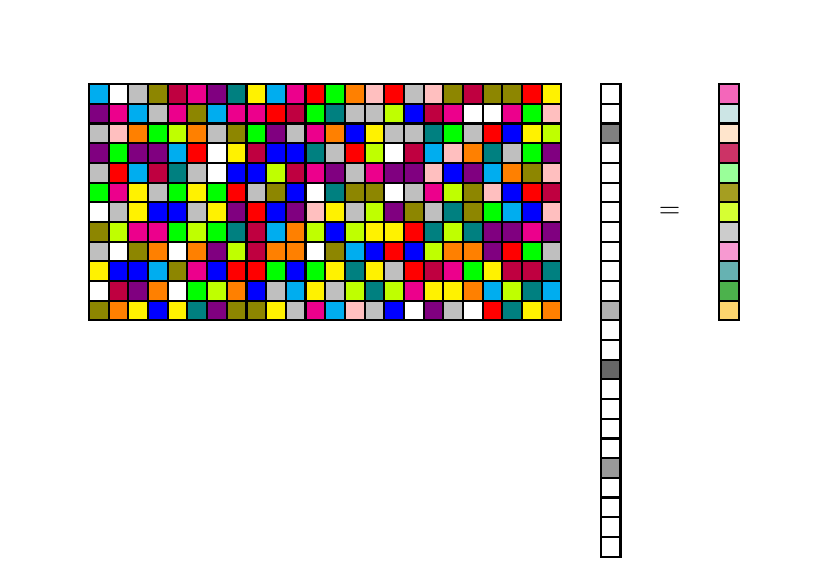
\begin{tikzpicture}
[draw=black, line width=0.75pt,
entry/.style={rectangle, draw, inner sep=0pt, minimum size=2.5mm},
symbol/.style={rectangle, draw, inner sep=0pt, minimum size=2.5mm}]

\node[entry, fill=olive] (x0y0) at (0.0,0.0) {};
\node[entry, fill=white] (x0y1) at (0.0,0.25) {};
\node[entry, fill=yellow] (x0y2) at (0.0,0.5) {};
\node[entry, fill=lightgray] (x0y3) at (0.0,0.75) {};
\node[entry, fill=olive] (x0y4) at (0.0,1.0) {};
\node[entry, fill=white] (x0y5) at (0.0,1.25) {};
\node[entry, fill=green] (x0y6) at (0.0,1.5) {};
\node[entry, fill=lightgray] (x0y7) at (0.0,1.75) {};
\node[entry, fill=violet] (x0y8) at (0.0,2.0) {};
\node[entry, fill=lightgray] (x0y9) at (0.0,2.25) {};
\node[entry, fill=violet] (x0y10) at (0.0,2.5) {};
\node[entry, fill=cyan] (x0y11) at (0.0,2.75) {};

\node[entry, fill=orange] (x1y0) at (0.25,0.0) {};
\node[entry, fill=purple] (x1y1) at (0.25,0.25) {};
\node[entry, fill=blue] (x1y2) at (0.25,0.5) {};
\node[entry, fill=white] (x1y3) at (0.25,0.75) {};
\node[entry, fill=lime] (x1y4) at (0.25,1.0) {};
\node[entry, fill=lightgray] (x1y5) at (0.25,1.25) {};
\node[entry, fill=magenta] (x1y6) at (0.25,1.5) {};
\node[entry, fill=red] (x1y7) at (0.25,1.75) {};
\node[entry, fill=green] (x1y8) at (0.25,2.0) {};
\node[entry, fill=pink] (x1y9) at (0.25,2.25) {};
\node[entry, fill=magenta] (x1y10) at (0.25,2.5) {};
\node[entry, fill=white] (x1y11) at (0.25,2.75) {};

\node[entry, fill=yellow] (x2y0) at (0.5,0.0) {};
\node[entry, fill=violet] (x2y1) at (0.5,0.25) {};
\node[entry, fill=blue] (x2y2) at (0.5,0.5) {};
\node[entry, fill=olive] (x2y3) at (0.5,0.75) {};
\node[entry, fill=magenta] (x2y4) at (0.5,1.0) {};
\node[entry, fill=yellow] (x2y5) at (0.5,1.25) {};
\node[entry, fill=yellow] (x2y6) at (0.5,1.5) {};
\node[entry, fill=cyan] (x2y7) at (0.5,1.75) {};
\node[entry, fill=violet] (x2y8) at (0.5,2.0) {};
\node[entry, fill=orange] (x2y9) at (0.5,2.25) {};
\node[entry, fill=cyan] (x2y10) at (0.5,2.5) {};
\node[entry, fill=lightgray] (x2y11) at (0.5,2.75) {};

\node[entry, fill=blue] (x3y0) at (0.75,0.0) {};
\node[entry, fill=orange] (x3y1) at (0.75,0.25) {};
\node[entry, fill=cyan] (x3y2) at (0.75,0.5) {};
\node[entry, fill=orange] (x3y3) at (0.75,0.75) {};
\node[entry, fill=magenta] (x3y4) at (0.75,1.0) {};
\node[entry, fill=blue] (x3y5) at (0.75,1.25) {};
\node[entry, fill=lightgray] (x3y6) at (0.75,1.5) {};
\node[entry, fill=purple] (x3y7) at (0.75,1.75) {};
\node[entry, fill=violet] (x3y8) at (0.75,2.0) {};
\node[entry, fill=green] (x3y9) at (0.75,2.25) {};
\node[entry, fill=lightgray] (x3y10) at (0.75,2.5) {};
\node[entry, fill=olive] (x3y11) at (0.75,2.75) {};

\node[entry, fill=yellow] (x4y0) at (1.0,0.0) {};
\node[entry, fill=white] (x4y1) at (1.0,0.25) {};
\node[entry, fill=olive] (x4y2) at (1.0,0.5) {};
\node[entry, fill=white] (x4y3) at (1.0,0.75) {};
\node[entry, fill=green] (x4y4) at (1.0,1.0) {};
\node[entry, fill=blue] (x4y5) at (1.0,1.25) {};
\node[entry, fill=green] (x4y6) at (1.0,1.5) {};
\node[entry, fill=teal] (x4y7) at (1.0,1.75) {};
\node[entry, fill=cyan] (x4y8) at (1.0,2.0) {};
\node[entry, fill=lime] (x4y9) at (1.0,2.25) {};
\node[entry, fill=magenta] (x4y10) at (1.0,2.5) {};
\node[entry, fill=purple] (x4y11) at (1.0,2.75) {};

\node[entry, fill=teal] (x5y0) at (1.25,0.0) {};
\node[entry, fill=green] (x5y1) at (1.25,0.25) {};
\node[entry, fill=magenta] (x5y2) at (1.25,0.5) {};
\node[entry, fill=orange] (x5y3) at (1.25,0.75) {};
\node[entry, fill=lime] (x5y4) at (1.25,1.0) {};
\node[entry, fill=lightgray] (x5y5) at (1.25,1.25) {};
\node[entry, fill=yellow] (x5y6) at (1.25,1.5) {};
\node[entry, fill=lightgray] (x5y7) at (1.25,1.75) {};
\node[entry, fill=red] (x5y8) at (1.25,2.0) {};
\node[entry, fill=orange] (x5y9) at (1.25,2.25) {};
\node[entry, fill=olive] (x5y10) at (1.25,2.5) {};
\node[entry, fill=magenta] (x5y11) at (1.25,2.75) {};

\node[entry, fill=violet] (x6y0) at (1.5,0.0) {};
\node[entry, fill=lime] (x6y1) at (1.5,0.25) {};
\node[entry, fill=blue] (x6y2) at (1.5,0.5) {};
\node[entry, fill=violet] (x6y3) at (1.5,0.75) {};
\node[entry, fill=green] (x6y4) at (1.5,1.0) {};
\node[entry, fill=yellow] (x6y5) at (1.5,1.25) {};
\node[entry, fill=green] (x6y6) at (1.5,1.5) {};
\node[entry, fill=white] (x6y7) at (1.5,1.75) {};
\node[entry, fill=white] (x6y8) at (1.5,2.0) {};
\node[entry, fill=lightgray] (x6y9) at (1.5,2.25) {};
\node[entry, fill=cyan] (x6y10) at (1.5,2.5) {};
\node[entry, fill=violet] (x6y11) at (1.5,2.75) {};

\node[entry, fill=olive] (x7y0) at (1.75,0.0) {};
\node[entry, fill=orange] (x7y1) at (1.75,0.25) {};
\node[entry, fill=red] (x7y2) at (1.75,0.5) {};
\node[entry, fill=lime] (x7y3) at (1.75,0.75) {};
\node[entry, fill=teal] (x7y4) at (1.75,1.0) {};
\node[entry, fill=violet] (x7y5) at (1.75,1.25) {};
\node[entry, fill=red] (x7y6) at (1.75,1.5) {};
\node[entry, fill=blue] (x7y7) at (1.75,1.75) {};
\node[entry, fill=yellow] (x7y8) at (1.75,2.0) {};
\node[entry, fill=olive] (x7y9) at (1.75,2.25) {};
\node[entry, fill=magenta] (x7y10) at (1.75,2.5) {};
\node[entry, fill=teal] (x7y11) at (1.75,2.75) {};

\node[entry, fill=olive] (x8y0) at (2.0,0.0) {};
\node[entry, fill=blue] (x8y1) at (2.0,0.25) {};
\node[entry, fill=red] (x8y2) at (2.0,0.5) {};
\node[entry, fill=purple] (x8y3) at (2.0,0.75) {};
\node[entry, fill=purple] (x8y4) at (2.0,1.0) {};
\node[entry, fill=red] (x8y5) at (2.0,1.25) {};
\node[entry, fill=lightgray] (x8y6) at (2.0,1.5) {};
\node[entry, fill=blue] (x8y7) at (2.0,1.75) {};
\node[entry, fill=purple] (x8y8) at (2.0,2.0) {};
\node[entry, fill=green] (x8y9) at (2.0,2.25) {};
\node[entry, fill=magenta] (x8y10) at (2.0,2.5) {};
\node[entry, fill=yellow] (x8y11) at (2.0,2.75) {};

\node[entry, fill=yellow] (x9y0) at (2.25,0.0) {};
\node[entry, fill=lightgray] (x9y1) at (2.25,0.25) {};
\node[entry, fill=green] (x9y2) at (2.25,0.5) {};
\node[entry, fill=orange] (x9y3) at (2.25,0.75) {};
\node[entry, fill=cyan] (x9y4) at (2.25,1.0) {};
\node[entry, fill=blue] (x9y5) at (2.25,1.25) {};
\node[entry, fill=olive] (x9y6) at (2.25,1.5) {};
\node[entry, fill=lime] (x9y7) at (2.25,1.75) {};
\node[entry, fill=blue] (x9y8) at (2.25,2.0) {};
\node[entry, fill=violet] (x9y9) at (2.25,2.25) {};
\node[entry, fill=red] (x9y10) at (2.25,2.5) {};
\node[entry, fill=cyan] (x9y11) at (2.25,2.75) {};

\node[entry, fill=lightgray] (x10y0) at (2.5,0.0) {};
\node[entry, fill=cyan] (x10y1) at (2.5,0.25) {};
\node[entry, fill=blue] (x10y2) at (2.5,0.5) {};
\node[entry, fill=orange] (x10y3) at (2.5,0.75) {};
\node[entry, fill=orange] (x10y4) at (2.5,1.0) {};
\node[entry, fill=violet] (x10y5) at (2.5,1.25) {};
\node[entry, fill=blue] (x10y6) at (2.5,1.5) {};
\node[entry, fill=purple] (x10y7) at (2.5,1.75) {};
\node[entry, fill=blue] (x10y8) at (2.5,2.0) {};
\node[entry, fill=lightgray] (x10y9) at (2.5,2.25) {};
\node[entry, fill=purple] (x10y10) at (2.5,2.5) {};
\node[entry, fill=magenta] (x10y11) at (2.5,2.75) {};

\node[entry, fill=magenta] (x11y0) at (2.75,0.0) {};
\node[entry, fill=yellow] (x11y1) at (2.75,0.25) {};
\node[entry, fill=green] (x11y2) at (2.75,0.5) {};
\node[entry, fill=white] (x11y3) at (2.75,0.75) {};
\node[entry, fill=lime] (x11y4) at (2.75,1.0) {};
\node[entry, fill=pink] (x11y5) at (2.75,1.25) {};
\node[entry, fill=white] (x11y6) at (2.75,1.5) {};
\node[entry, fill=magenta] (x11y7) at (2.75,1.75) {};
\node[entry, fill=teal] (x11y8) at (2.75,2.0) {};
\node[entry, fill=magenta] (x11y9) at (2.75,2.25) {};
\node[entry, fill=green] (x11y10) at (2.75,2.5) {};
\node[entry, fill=red] (x11y11) at (2.75,2.75) {};

\node[entry, fill=cyan] (x12y0) at (3.0,0.0) {};
\node[entry, fill=lightgray] (x12y1) at (3.0,0.25) {};
\node[entry, fill=yellow] (x12y2) at (3.0,0.5) {};
\node[entry, fill=olive] (x12y3) at (3.0,0.75) {};
\node[entry, fill=blue] (x12y4) at (3.0,1.0) {};
\node[entry, fill=yellow] (x12y5) at (3.0,1.25) {};
\node[entry, fill=teal] (x12y6) at (3.0,1.5) {};
\node[entry, fill=violet] (x12y7) at (3.0,1.75) {};
\node[entry, fill=lightgray] (x12y8) at (3.0,2.0) {};
\node[entry, fill=orange] (x12y9) at (3.0,2.25) {};
\node[entry, fill=teal] (x12y10) at (3.0,2.5) {};
\node[entry, fill=green] (x12y11) at (3.0,2.75) {};

\node[entry, fill=pink] (x13y0) at (3.25,0.0) {};
\node[entry, fill=lime] (x13y1) at (3.25,0.25) {};
\node[entry, fill=teal] (x13y2) at (3.25,0.5) {};
\node[entry, fill=cyan] (x13y3) at (3.25,0.75) {};
\node[entry, fill=lime] (x13y4) at (3.25,1.0) {};
\node[entry, fill=lightgray] (x13y5) at (3.25,1.25) {};
\node[entry, fill=olive] (x13y6) at (3.25,1.5) {};
\node[entry, fill=lightgray] (x13y7) at (3.25,1.75) {};
\node[entry, fill=red] (x13y8) at (3.25,2.0) {};
\node[entry, fill=blue] (x13y9) at (3.25,2.25) {};
\node[entry, fill=lightgray] (x13y10) at (3.25,2.5) {};
\node[entry, fill=orange] (x13y11) at (3.25,2.75) {};

\node[entry, fill=lightgray] (x14y0) at (3.5,0.0) {};
\node[entry, fill=teal] (x14y1) at (3.5,0.25) {};
\node[entry, fill=yellow] (x14y2) at (3.5,0.5) {};
\node[entry, fill=blue] (x14y3) at (3.5,0.75) {};
\node[entry, fill=yellow] (x14y4) at (3.5,1.0) {};
\node[entry, fill=lime] (x14y5) at (3.5,1.25) {};
\node[entry, fill=olive] (x14y6) at (3.5,1.5) {};
\node[entry, fill=magenta] (x14y7) at (3.5,1.75) {};
\node[entry, fill=lime] (x14y8) at (3.5,2.0) {};
\node[entry, fill=yellow] (x14y9) at (3.5,2.25) {};
\node[entry, fill=lightgray] (x14y10) at (3.5,2.5) {};
\node[entry, fill=pink] (x14y11) at (3.5,2.75) {};

\node[entry, fill=blue] (x15y0) at (3.75,0.0) {};
\node[entry, fill=lime] (x15y1) at (3.75,0.25) {};
\node[entry, fill=lightgray] (x15y2) at (3.75,0.5) {};
\node[entry, fill=red] (x15y3) at (3.75,0.75) {};
\node[entry, fill=yellow] (x15y4) at (3.75,1.0) {};
\node[entry, fill=violet] (x15y5) at (3.75,1.25) {};
\node[entry, fill=white] (x15y6) at (3.75,1.5) {};
\node[entry, fill=violet] (x15y7) at (3.75,1.75) {};
\node[entry, fill=white] (x15y8) at (3.75,2.0) {};
\node[entry, fill=lightgray] (x15y9) at (3.75,2.25) {};
\node[entry, fill=lime] (x15y10) at (3.75,2.5) {};
\node[entry, fill=red] (x15y11) at (3.75,2.75) {};

\node[entry, fill=white] (x16y0) at (4.0,0.0) {};
\node[entry, fill=magenta] (x16y1) at (4.0,0.25) {};
\node[entry, fill=red] (x16y2) at (4.0,0.5) {};
\node[entry, fill=blue] (x16y3) at (4.0,0.75) {};
\node[entry, fill=red] (x16y4) at (4.0,1.0) {};
\node[entry, fill=olive] (x16y5) at (4.0,1.25) {};
\node[entry, fill=lightgray] (x16y6) at (4.0,1.5) {};
\node[entry, fill=violet] (x16y7) at (4.0,1.75) {};
\node[entry, fill=purple] (x16y8) at (4.0,2.0) {};
\node[entry, fill=lightgray] (x16y9) at (4.0,2.25) {};
\node[entry, fill=blue] (x16y10) at (4.0,2.5) {};
\node[entry, fill=lightgray] (x16y11) at (4.0,2.75) {};

\node[entry, fill=violet] (x17y0) at (4.25,0.0) {};
\node[entry, fill=yellow] (x17y1) at (4.25,0.25) {};
\node[entry, fill=purple] (x17y2) at (4.25,0.5) {};
\node[entry, fill=lime] (x17y3) at (4.25,0.75) {};
\node[entry, fill=teal] (x17y4) at (4.25,1.0) {};
\node[entry, fill=lightgray] (x17y5) at (4.25,1.25) {};
\node[entry, fill=magenta] (x17y6) at (4.25,1.5) {};
\node[entry, fill=pink] (x17y7) at (4.25,1.75) {};
\node[entry, fill=cyan] (x17y8) at (4.25,2.0) {};
\node[entry, fill=teal] (x17y9) at (4.25,2.25) {};
\node[entry, fill=purple] (x17y10) at (4.25,2.5) {};
\node[entry, fill=pink] (x17y11) at (4.25,2.75) {};

\node[entry, fill=lightgray] (x18y0) at (4.5,0.0) {};
\node[entry, fill=yellow] (x18y1) at (4.5,0.25) {};
\node[entry, fill=magenta] (x18y2) at (4.5,0.5) {};
\node[entry, fill=orange] (x18y3) at (4.5,0.75) {};
\node[entry, fill=lime] (x18y4) at (4.5,1.0) {};
\node[entry, fill=teal] (x18y5) at (4.5,1.25) {};
\node[entry, fill=lime] (x18y6) at (4.5,1.5) {};
\node[entry, fill=blue] (x18y7) at (4.5,1.75) {};
\node[entry, fill=pink] (x18y8) at (4.5,2.0) {};
\node[entry, fill=green] (x18y9) at (4.5,2.25) {};
\node[entry, fill=magenta] (x18y10) at (4.5,2.5) {};
\node[entry, fill=olive] (x18y11) at (4.5,2.75) {};

\node[entry, fill=white] (x19y0) at (4.75,0.0) {};
\node[entry, fill=orange] (x19y1) at (4.75,0.25) {};
\node[entry, fill=green] (x19y2) at (4.75,0.5) {};
\node[entry, fill=orange] (x19y3) at (4.75,0.75) {};
\node[entry, fill=teal] (x19y4) at (4.75,1.0) {};
\node[entry, fill=olive] (x19y5) at (4.75,1.25) {};
\node[entry, fill=olive] (x19y6) at (4.75,1.5) {};
\node[entry, fill=violet] (x19y7) at (4.75,1.75) {};
\node[entry, fill=orange] (x19y8) at (4.75,2.0) {};
\node[entry, fill=lightgray] (x19y9) at (4.75,2.25) {};
\node[entry, fill=white] (x19y10) at (4.75,2.5) {};
\node[entry, fill=purple] (x19y11) at (4.75,2.75) {};

\node[entry, fill=red] (x20y0) at (5.0,0.0) {};
\node[entry, fill=cyan] (x20y1) at (5.0,0.25) {};
\node[entry, fill=yellow] (x20y2) at (5.0,0.5) {};
\node[entry, fill=violet] (x20y3) at (5.0,0.75) {};
\node[entry, fill=violet] (x20y4) at (5.0,1.0) {};
\node[entry, fill=green] (x20y5) at (5.0,1.25) {};
\node[entry, fill=pink] (x20y6) at (5.0,1.5) {};
\node[entry, fill=cyan] (x20y7) at (5.0,1.75) {};
\node[entry, fill=teal] (x20y8) at (5.0,2.0) {};
\node[entry, fill=red] (x20y9) at (5.0,2.25) {};
\node[entry, fill=white] (x20y10) at (5.0,2.5) {};
\node[entry, fill=olive] (x20y11) at (5.0,2.75) {};

\node[entry, fill=teal] (x21y0) at (5.25,0.0) {};
\node[entry, fill=lime] (x21y1) at (5.25,0.25) {};
\node[entry, fill=purple] (x21y2) at (5.25,0.5) {};
\node[entry, fill=red] (x21y3) at (5.25,0.75) {};
\node[entry, fill=violet] (x21y4) at (5.25,1.0) {};
\node[entry, fill=cyan] (x21y5) at (5.25,1.25) {};
\node[entry, fill=blue] (x21y6) at (5.25,1.5) {};
\node[entry, fill=orange] (x21y7) at (5.25,1.75) {};
\node[entry, fill=lightgray] (x21y8) at (5.25,2.0) {};
\node[entry, fill=blue] (x21y9) at (5.25,2.25) {};
\node[entry, fill=magenta] (x21y10) at (5.25,2.5) {};
\node[entry, fill=olive] (x21y11) at (5.25,2.75) {};

\node[entry, fill=yellow] (x22y0) at (5.5,0.0) {};
\node[entry, fill=teal] (x22y1) at (5.5,0.25) {};
\node[entry, fill=purple] (x22y2) at (5.5,0.5) {};
\node[entry, fill=green] (x22y3) at (5.5,0.75) {};
\node[entry, fill=magenta] (x22y4) at (5.5,1.0) {};
\node[entry, fill=blue] (x22y5) at (5.5,1.25) {};
\node[entry, fill=red] (x22y6) at (5.5,1.5) {};
\node[entry, fill=olive] (x22y7) at (5.5,1.75) {};
\node[entry, fill=green] (x22y8) at (5.5,2.0) {};
\node[entry, fill=yellow] (x22y9) at (5.5,2.25) {};
\node[entry, fill=green] (x22y10) at (5.5,2.5) {};
\node[entry, fill=red] (x22y11) at (5.5,2.75) {};

\node[entry, fill=orange] (x23y0) at (5.75,0.0) {};
\node[entry, fill=cyan] (x23y1) at (5.75,0.25) {};
\node[entry, fill=teal] (x23y2) at (5.75,0.5) {};
\node[entry, fill=lightgray] (x23y3) at (5.75,0.75) {};
\node[entry, fill=violet] (x23y4) at (5.75,1.0) {};
\node[entry, fill=pink] (x23y5) at (5.75,1.25) {};
\node[entry, fill=purple] (x23y6) at (5.75,1.5) {};
\node[entry, fill=pink] (x23y7) at (5.75,1.75) {};
\node[entry, fill=violet] (x23y8) at (5.75,2.0) {};
\node[entry, fill=lime] (x23y9) at (5.75,2.25) {};
\node[entry, fill=pink] (x23y10) at (5.75,2.5) {};
\node[entry, fill=yellow] (x23y11) at (5.75,2.75) {};


\node[symbol] (s01) at (6.5,-3.00) {};
\node[symbol] (s02) at (6.5,-2.75) {};
\node[symbol] (s03) at (6.5,-2.50) {};
\node[symbol] (s04) at (6.5,-2.25) {};
\node[symbol,fill=black!40] (s05) at (6.5,-2.00) {};
\node[symbol] (s06) at (6.5,-1.75) {};
\node[symbol] (s07) at (6.5,-1.50) {};
\node[symbol] (s08) at (6.5,-1.25) {};
\node[symbol] (s09) at (6.5,-1.00) {};
\node[symbol,fill=black!60] (s10) at (6.5,-0.75) {};
\node[symbol] (s11) at (6.5,-0.50) {};
\node[symbol] (s12) at (6.5,-0.25) {};
\node[symbol,fill=black!30] (s13) at (6.5,0) {};
\node[symbol] (s14) at (6.5,0.25) {};
\node[symbol] (s15) at (6.5,0.50) {};
\node[symbol] (s16) at (6.5,0.75) {};
\node[symbol] (s17) at (6.5,1.00) {};
\node[symbol] (s18) at (6.5,1.25) {};
\node[symbol] (s19) at (6.5,1.50) {};
\node[symbol] (s20) at (6.5,1.75) {};
\node[symbol] (s21) at (6.5,2.00) {};
\node[symbol,fill=black!50] (s22) at (6.5,2.25) {};
\node[symbol] (s23) at (6.5,2.50) {};
\node[symbol] (s24) at (6.5,2.75) {};

\node (equal) at (7.25,1.25) {$=$};

\node[entry, fill=yellow!40!pink] (o0) at (8,0.0) {};
\node[entry, fill=gray!60!green] (o1) at (8,0.25) {};
\node[entry, fill=teal!60] (o2) at (8,0.5) {};
\node[entry, fill=magenta!40] (o3) at (8,0.75) {};
\node[entry, fill=gray!40] (o4) at (8,1.0) {};
\node[entry, fill=green!20!yellow!80] (o5) at (8,1.25) {};
\node[entry, fill=olive!80] (o6) at (8,1.5) {};
\node[entry, fill=green!40] (o7) at (8,1.75) {};
\node[entry, fill=purple!80] (o8) at (8,2.0) {};
\node[entry, fill=orange!20] (o9) at (8,2.25) {};
\node[entry, fill=teal!20] (o10) at (8,2.5) {};
\node[entry, fill=magenta!60] (o11) at (8,2.75) {};


\draw[|-|,opacity=0] (-0.125, 3.125) to node[above] {\small Number of columns} (5.875, 3.125);
\draw[|-|,opacity=0] (-0.375, -0.125) to node[above,rotate=90] {\small Number of samples} (-0.375, 2.875);
\draw[|-|,opacity=0] (6.875, -3.125) to node[above,rotate=-90] {\small Number of non-zero entries} (6.875, 2.875);
\node[opacity=0] (framework) at (2.875,-0.5) {Sensing matrix $\boldsymbol{\Phi}$};
\node[rotate=-90,opacity=0] (vector) at (7,-0.75) {Sparse vector $\mathbf{s}$};
\node[rotate=-90,opacity=0] (observation) at (8.5,1.5) {Observation $\mathbf{y}$};

% \node[text width=5cm] (equation) at (2.875, -1.625) {Undersampling faction $\delta$: \[ \frac{\text{height of } \boldsymbol{\Phi}}{\text{width of } \boldsymbol{\Phi}} = \frac{n}{N} \rightarrow \delta \]};
% \node[text width=5cm] (equation) at (2.875, -1.625) {Measure of sparsity $\rho$: \[ \frac{\text{Signal complexity } \left\| \mathbf{s} \right\|_0 }{\text{height of } \boldsymbol{\Phi}} = \frac{K}{n} \rightarrow \rho \]};
% \node[text width=5cm] (width) at (2.875, -1.625) {Sampling complexity: \[ c \cdot K \log \frac{N}{K} \]};

\end{tikzpicture}
}
\begin{itemize}
\item $\vec{y} = A \vec{x} + \vec{z} \quad \text{with} \quad \|\vec{x}\|_0 = K$
\item Dimensionality of CS problem is \textbf{huge}
\item Computational complexity of conventional CS solvers: $\mathcal{O}(\mathrm{poly}(2^B))$
\end{itemize}
\end{frame}



\part{A Quest for Low-Complexity: \newline Sparsifying Collision}
\frame{\partpage}


\begin{frame}
\frametitle{Quest for Low-Complexity Unsourced MAC}

\begin{block}{Idea~1: Stochastic Binning}
\begin{center}
  \scalebox{0.8}{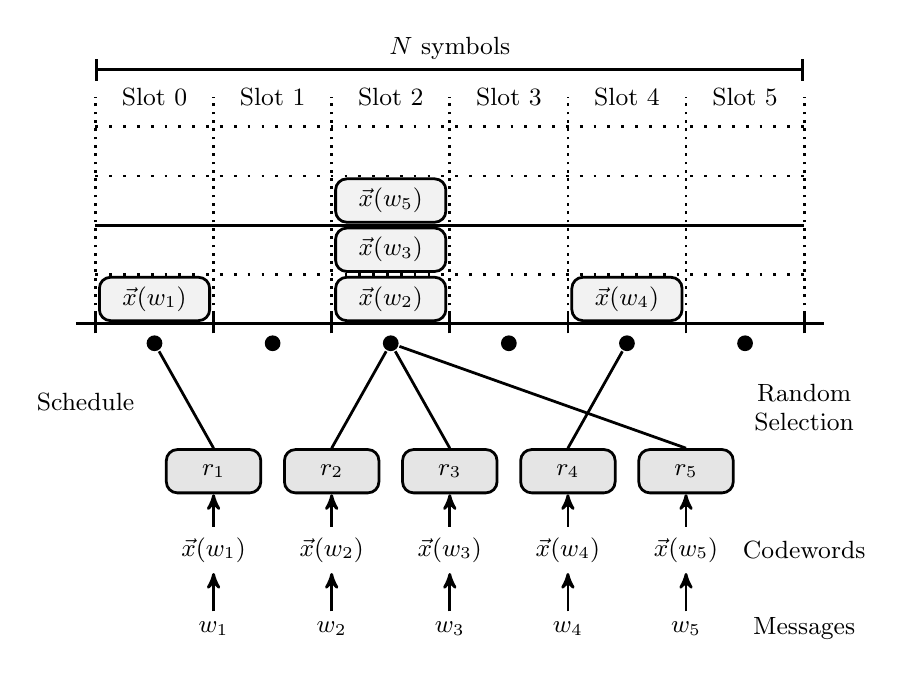
\begin{tikzpicture}[
  font=\small, >=stealth',line width=1pt,
  slot/.style={circle, minimum height = 2mm, fill=black, inner sep=0pt},
  scheduler/.style={rectangle, minimum height=5.5mm, minimum width=12mm, draw=black, fill=gray!20, rounded corners},
  packet/.style={rectangle, minimum height=5.5mm, minimum width=14mm, draw=black, fill=gray!10, rounded corners}
]

\draw [|-|] (0,8.6) to node[midway,above] {$N$ symbols} (9,8.6);

\draw [-] (-0.25,5.375) -- (9.25,5.375);
\foreach \t in {0,...,6} {
  \draw (1.5*\t,5.25) -- (1.5*\t,5.5);
  \draw[dotted] (1.5*\t,5.5) -- (1.5*\t,8.25);
}

\draw [-] (0,6.625) -- (9,6.625);
\foreach \l in {1,...,4} {
  \draw[loosely dotted] (0,5.375+0.625*\l) -- (9,5.375+0.625*\l);
}

\foreach \s in {0,...,5} {
  \node[slot] (s\s) at (0.75+1.5*\s,5.125) {};
}

\foreach \s in {0,...,5} {
  \node (t\s) at (0.75+1.5*\s,8.25) {Slot~\s};
}

\node (schedulers1) at (-0.125,4.375) {Schedule};
\node[scheduler] (d5) at (7.5,3.5) {$r_5$};
\node[scheduler] (d4) at (6.0,3.5) {$r_4$};
\node[scheduler] (d3) at (4.5,3.5) {$r_3$};
\node[scheduler] (d2) at (3.0,3.5) {$r_2$};
\node[scheduler] (d1) at (1.5,3.5) {$r_1$};
\node (codewords1) at (9,4.5) {Random};
\node (codewords2) at (9,4.125) {Selection};

\node (codewords1) at (9,2.5) {Codewords};
\node (c5) at (7.5,2.5) {$\vec{x}(w_5)$};
\node (c4) at (6.0,2.5) {$\vec{x}(w_4)$};
\node (c3) at (4.5,2.5) {$\vec{x}(w_3)$};
\node (c2) at (3.0,2.5) {$\vec{x}(w_2)$};
\node (c1) at (1.5,2.5) {$\vec{x}(w_1)$};

\node (messages) at (9,1.5) {Messages};
\node (m5) at (7.5,1.5) {$w_5$};
\node (m4) at (6.0,1.5) {$w_4$};
\node (m3) at (4.5,1.5) {$w_3$};
\node (m2) at (3.0,1.5) {$w_2$};
\node (m1) at (1.5,1.5) {$w_1$};

\draw[->] (m1) -- (c1);
\draw[->] (m2) -- (c2);
\draw[->] (m3) -- (c3);
\draw[->] (m4) -- (c4);
\draw[->] (m5) -- (c5);

\draw[->] (c1) -- (d1.south);
\draw[->] (c2) -- (d2.south);
\draw[->] (c3) -- (d3.south);
\draw[->] (c4) -- (d4.south);
\draw[->] (c5) -- (d5.south);

\draw (d5.north) -- (s2);
\draw (d4.north) -- (s4);
\draw (d3.north) -- (s2);
\draw (d2.north) -- (s2);
\draw (d1.north) -- (s0);

\node[packet] (p10) at (0.75,5.6875) {$\vec{x}(w_1)$};

\node[packet] (p42) at (3.75,6.9375) {$\vec{x}(w_5)$};
\node[packet] (p32) at (3.75,6.3125) {$\vec{x}(w_3)$};
\node[packet] (p22) at (3.75,5.6875) {$\vec{x}(w_2)$};

\node[packet] (p44) at (6.75,5.6875) {$\vec{x}(w_4)$};
\end{tikzpicture}
}
\end{center}
\end{block}
\myfootnote{\tiny
O. Ordentlich and Y. Polyanskiy. \emph{Low Complexity Schemes for the Random Access Gaussian Channel}. ISIT, 2017}
\end{frame}

\begin{frame}
\frametitle{Caveat -- The Poisson Wall}

\begin{columns}
\column{.48\textwidth}
  \begin{center}
  \scalebox{1.0}{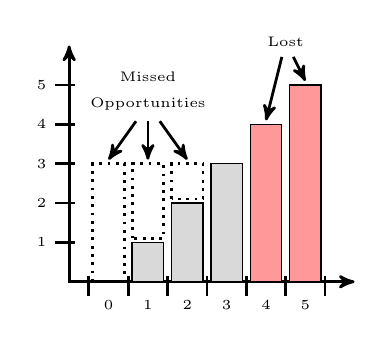
\begin{tikzpicture}[
  font=\tiny, >=stealth', line width=1pt
]

\draw [<->] (-0.25,3) -- (-0.25,0) -- (3.375,0);
\foreach \x in {0,...,6} {
  \draw (0.5*\x,-0.175) -- (0.5*\x,0.075);
}
\foreach \x in {0,1,...,5} {
  \node (tx\x) at (0.5*\x+0.25,-0.3) {\x};
}
\foreach \y in {1,...,5} {
  \draw (-0.425,0.5*\y) -- (-0.175,0.5*\y);
}
\foreach \y in {1,...,5} {
  \node (ty\y) at (-0.6,0.5*\y) {\y};
}

\draw[dotted] (0.05,0) rectangle (0.45,1.5);
\draw[fill=gray!30,line width=0.5pt] (0.55,0) rectangle (0.95,0.5);
\draw[dotted] (0.55,0.55) rectangle (0.95,1.5);
\draw[fill=gray!30,line width=0.5pt] (1.05,0) rectangle (1.45,1);
\draw[dotted] (1.05,1.05) rectangle (1.45,1.5);
\draw[fill=gray!30,line width=0.5pt] (1.55,0) rectangle (1.95,1.5);
\draw[fill=red!40,line width=0.5pt] (2.05,0) rectangle (2.45,2);
\draw[fill=red!40,line width=0.5pt] (2.55,0) rectangle (2.95,2.5);

\node (under0) at (0.75,2.6) {Missed};
\node (under1) at (0.75,2.25) {Opportunities};
\draw[->] (under1) -- (0.25,1.55);
\draw[->] (under1) -- (0.75,1.55);
\draw[->] (under1) -- (1.25,1.55);

\node (over) at (2.5,3.05) {Lost};
\draw[->] (over) -- (2.25,2.05);
\draw[->] (over) -- (2.75,2.55);
\end{tikzpicture}
} \\
  \textcolor{gray}{\scriptsize Sum Reward}
  \end{center}
\column{.48\textwidth}
  \begin{center}
  \scalebox{1.0}{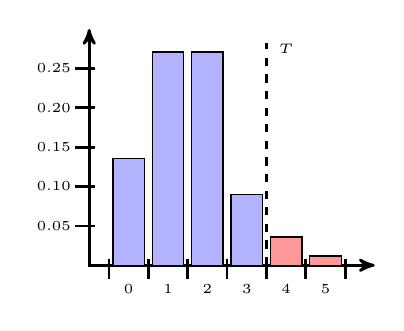
\begin{tikzpicture}[
  font=\tiny, >=stealth', line width=1pt
]

\draw [<->] (-0.25,3) -- (-0.25,0) -- (3.375,0);
\foreach \x in {0,...,6} {
  \draw (0.5*\x,-0.175) -- (0.5*\x,0.075);
}
\foreach \x in {0,1,...,5} {
  \node (tx\x) at (0.5*\x+0.25,-0.3) {\x};
}
\foreach \y in {1,...,5} {
  \draw (-0.425,0.5*\y) -- (-0.175,0.5*\y);
}
\foreach \y in {0.05,0.10,0.15,0.20,0.25} {
  \node (ty\y) at (-0.7,10*\y) {\y};
}

\draw[dashed] (2,0) -- (2,2.825);
\node at (2.25,2.75) {$T$};

\draw[fill=blue!30,line width=0.5pt] (0.05,0) rectangle (0.45,1.353);
\draw[fill=blue!30,line width=0.5pt] (0.55,0) rectangle (0.95,2.707);
\draw[fill=blue!30,line width=0.5pt] (1.05,0) rectangle (1.45,2.707);
\draw[fill=blue!30,line width=0.5pt] (1.55,0) rectangle (1.95,0.902);
\draw[fill=red!40,line width=0.5pt] (2.05,0) rectangle (2.45,0.361);
\draw[fill=red!40,line width=0.5pt] (2.55,0) rectangle (2.95,0.120);

\end{tikzpicture}
} \\
  \textcolor{gray}{\scriptsize Count Distribution}
\end{center}
\end{columns}
\vfill
\begin{columns}
\column{.53\textwidth}
\begin{block}{Effects of Decoding Threshold}
  \begin{itemize}
  \item More slots reduces parameter of Poisson/binomial distribution
  \item More slots reduces bit count per decoded slot
  \end{itemize}
  \begin{footnotesize}
  \begin{equation*}
  \textstyle \sum_{k=0}^T
  \frac{N}{J} \frac{k}{T} \log_2 \left( 1 + J T \cdot \mathrm{SNR} \right)
  \mathrm{pmf}(k)
  \end{equation*}
  \end{footnotesize}
\end{block}
\column{.45\textwidth}
  \centerline{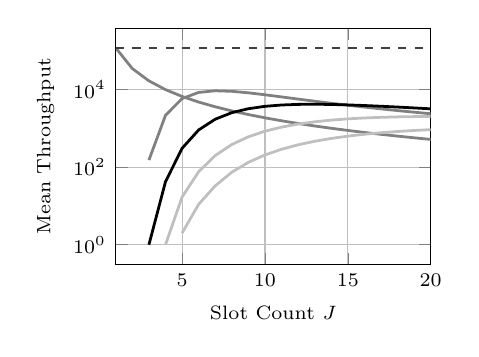
\begin{tikzpicture}
\begin{semilogyaxis}[
font=\scriptsize,
width=4cm,
height=3cm,
scale only axis,
xmin=1,
xmax=20,
xlabel={Slot Count $J$},
xmajorgrids,
ylabel={Mean Throughput},
ylabel near ticks,
ymajorgrids,
legend style={font=\tiny, at={(1,0)},anchor=south east, draw=black,fill=white,legend cell align=right}
]

\addplot [color=gray,solid,line width=1.0pt]
coordinates{
(1, 117955)
(2, 34614)
(3, 16724)
(4, 9944)
(5, 6631)
(6, 4756)
(7, 3588)
(8, 2810)
(9, 2264)
(10, 1865)
(11, 1565)
(12, 1333)
(13, 1150)
(14, 1003)
(15, 883)
(16, 783)
(17, 700)
(18, 630)
(19, 570)
(20, 518)
};
%\addlegendentry{$T$};

\addplot [color=gray,solid,line width=1.0pt]
coordinates{
%(1, 0)
%(1, 0)
%(2, 0)
(3, 152)
(4, 2158)
(5, 5824)
(6, 8417)
(7, 9267)
(8, 8992)
(9, 8222)
(10, 7318)
(11, 6447)
(12, 5669)
(13, 4997)
(14, 4423)
(15, 3936)
(16, 3522)
(17, 3168)
(18, 2865)
(19, 2603)
(20, 2375)
};
%\addlegendentry{$T=8$};


\addplot [color=black,solid,line width=1.0pt]
coordinates{
%(1, 0)
%(2, 0)
(3, 1)
(4, 42)
(5, 305)
(6, 907)
(7, 1718)
(8, 2529)
(9, 3202)
(10, 3687)
(11, 3989)
(12, 4138)
(13, 4171)
(14, 4120)
(15, 4013)
(16, 3870)
(17, 3705)
(18, 3531)
(19, 3353)
(20, 3178)
};
%\addlegendentry{$T=4$};

\addplot [color=lightgray,solid,line width=1.0pt]
  coordinates{
%(1, 0)
%(2, 0)
%(3, 0)
(4, 1)
(5, 17)
(6, 76)
(7, 199)
(8, 383)
(9, 605)
(10, 843)
(11, 1074)
(12, 1287)
(13, 1472)
(14, 1627)
(15, 1753)
(16, 1850)
(17, 1922)
(18, 1972)
(19, 2003)
(20, 2018)
};
%\addlegendentry{$T=2$};

\addplot [color=lightgray,solid,line width=1.0pt]
  coordinates{
%(1, 0)
%(2, 0)
%(3, 0)
%(4, 0)
(5, 2)
(6, 11)
(7, 33)
(8, 74)
(9, 133)
(10, 206)
(11, 289)
(12, 376)
(13, 464)
(14, 549)
(15, 629)
(16, 703)
(17, 769)
(18, 828)
(19, 880)
(20, 925)
};
%\addlegendentry{$T=1$};

\addplot [color=darkgray,dashed,line width=1.0pt,mark size=1.4pt]
  coordinates{
(1, 117955)
(2, 117955)
(3, 117955)
(4, 117955)
(5, 117955)
(6, 117955)
(7, 117955)
(8, 117955)
(9, 117955)
(10, 117955)
(11, 117955)
(12, 117955)
(13, 117955)
(14, 117955)
(15, 117955)
(16, 117955)
(17, 117955)
(18, 117955)
(19, 117955)
(20, 117955)
};

\end{semilogyaxis}
\end{tikzpicture}
}
\end{columns}
\end{frame}


\begin{frame}
\frametitle{Quest for Low-Complexity Unsourced MAC}

\begin{block}{Idea~1$++$: Slotted with Successive Interference Cancellation}
\centerline{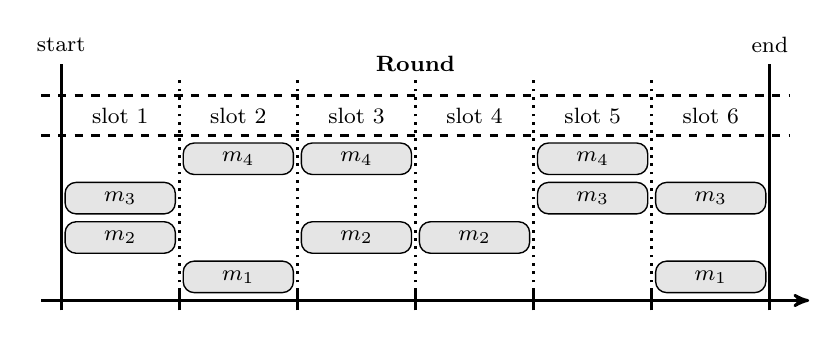
\begin{tikzpicture}[
  font=\footnotesize,
  >=stealth',
  line width=1pt,
  packet/.style={rectangle, minimum height=4mm, minimum width=14mm, draw=black, fill=gray!20, rounded corners, line width=0.5pt}
]

\draw [->] (0,-0.05) -- (9.75,-0.05);
\draw (0.25,-0.175) -- (0.25,2.95);
\foreach \x in {1,...,5} {
  \draw (1.5*\x+0.25,-0.175) -- (1.5*\x+0.25,0.075);
  \draw[dotted] (1.5*\x+0.25,0.075) -- (1.5*\x+0.25,2.75);
}
\draw (9.25,-0.175) -- (9.25,2.95);
\draw[dashed] (0,2.05) -- (9.5,2.05);
\draw[dashed] (0,2.55) -- (9.5,2.55);

\foreach \x in {1,...,6} {
  \node (t\x) at (1.5*\x-0.5,2.3) {slot~\x};
}
\node (round) at (4.75,2.95) {\textbf{Round}};
\node (start) at (0.25,3.2) {start};
\node (end) at (9.25,3.2) {end};

\node[packet] (p12) at (2.5,0.25) {$m_1$};
\node[packet] (p16) at (8.5,0.25) {$m_1$};
\node[packet] (p21) at (1.0,0.75) {$m_2$};
\node[packet] (p23) at (4.0,0.75) {$m_2$};
\node[packet] (p24) at (5.5,0.75) {$m_2$};
\node[packet] (p31) at (1.0,1.25) {$m_3$};
\node[packet] (p35) at (7.0,1.25) {$m_3$};
\node[packet] (p36) at (8.5,1.25) {$m_3$};
\node[packet] (p42) at (2.5,1.75) {$m_4$};
\node[packet] (p43) at (4.0,1.75) {$m_4$};
\node[packet] (p45) at (7.0,1.75) {$m_4$};

\end{tikzpicture}

}
\end{block}

\begin{block}{Leveraging Prior Work on Uncoordinated Access}
  \begin{itemize}
  \item $K$ \textbf{uncoordinated} devices, each with one packet to send
  \item Time is \textbf{slotted}; transmissions occur within slots
  \item Successive interference cancellation
  \end{itemize}
\end{block}

\myfootnote{\tiny
E. Casini, R. De Gaudenzi, and O. Del Rio Herrero. \emph{Contention resolution diversity slotted ALOHA (CRDSA): An enhanced random access scheme for satellite access packet networks}. IEEE Trans on Wireless Comm, 2007}
\myfootnote{\tiny
E Paolini, G Liva, M Chiani. \emph{Coded slotted ALOHA: A graph-based method for uncoordinated multiple access}.  IEEE Trans on Info Theory, 2015}
\end{frame}


\begin{frame}
\frametitle{Amenable to Graphical Representation}
\begin{itemize}
\item Tanner graph representation for transmission scheme
\item Variable nodes $\leftrightarrow$ packets;
check nodes $\leftrightarrow$ received signals
\item Message-passing decoder $\leftrightarrow$ peeling decoder for erasure channel
\end{itemize}
\begin{columns}
\column{.48\textwidth}
  \begin{center}
  \scalebox{0.8}{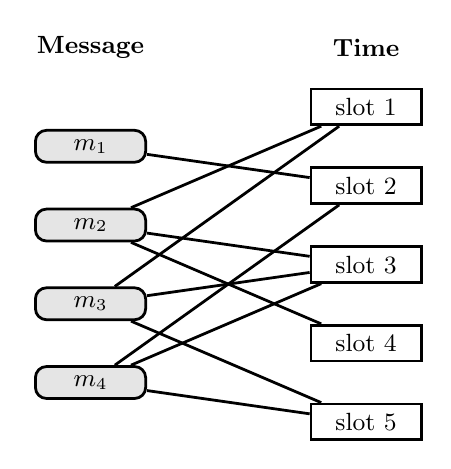
\begin{tikzpicture}
  [
  font=\small, line width=1pt, draw=black,
  checknode/.style={rectangle, minimum height=4mm, minimum width=14mm, draw=black},
  packet/.style={rectangle, minimum height=4mm, minimum width=14mm, draw=black, fill=gray!20, rounded corners}
  ]

\foreach \m in {1,2,3,4} {
  \node[packet] (v\m) at (0,0.5-\m) {$m_{\m}$};
}
  
\foreach \s in {1,2,3,4,5} {
  \node[checknode] (c\s) at (3.5,1-\s) {slot~\s};
}

\node (message) at (0,0.75) {\textbf{Message}};
\node (time) at (3.5,0.75) {\textbf{Time}};

\draw (v1) -- (c2);
\draw (v2) -- (c1);
\draw (v2) -- (c3);
\draw (v2) -- (c4);
\draw (v3) -- (c1);
\draw (v3) -- (c3);
\draw (v3) -- (c5);
\draw (v4) -- (c2);
\draw (v4) -- (c3);
\draw (v4) -- (c5);
\end{tikzpicture}
}
  \end{center}
\column{.48\textwidth}
  \begin{center}
  \scalebox{0.8}{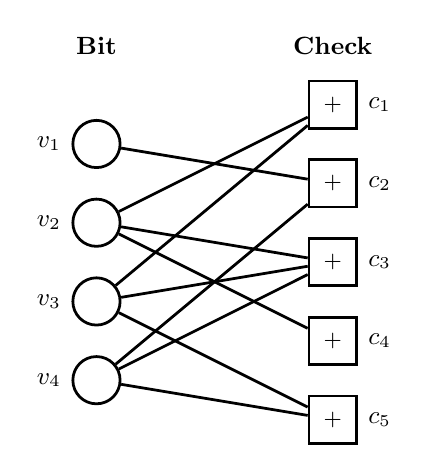
\begin{tikzpicture}
  [
  font=\small, line width=1pt, draw=black,
  bitnode/.style={circle, inner sep = 0pt, minimum size = 6mm, draw=black},
  checknode/.style={rectangle, inner sep = 0pt, minimum size = 6mm, draw=black},
  ]

\foreach \v in {1,2,3,4} {
  \node[bitnode] (v\v) at (0,0.5-\v) [label=left:$v_\v$]{};
}
  
\foreach \c in {1,2,3,4,5} {
  \node[checknode] (c\c) at (3,1-\c) [label=right:$c_\c$]{\footnotesize{$+$}};
}

\node (bit) at (0,0.75) {\textbf{Bit}};
\node (check) at (3,0.75) {\textbf{Check}};

\draw (v1) -- (c2);
\draw (v2) -- (c1);
\draw (v2) -- (c3);
\draw (v2) -- (c4);
\draw (v3) -- (c1);
\draw (v3) -- (c3);
\draw (v3) -- (c5);
\draw (v4) -- (c2);
\draw (v4) -- (c3);
\draw (v4) -- (c5);
\end{tikzpicture}

}
  \end{center}
\end{columns}
\myfootnote{\tiny
G. Liva. \emph{Graph-based analysis and optimization of contention resolution diversity slotted ALOHA}. IEEE Trans on Comm, 2011}
\myfootnote{\tiny
E. Paolini, G. Liva, and M. Chiani. \emph{Coded slotted ALOHA: A graph-based method for uncoordinated multiple access}. IEEE Trans on Info Theory, 2015}
\end{frame}


\begin{frame}
\frametitle{Decoder -- Peeling Algorithm}
\begin{block}{Joint decoding via successive interference cancellation}
  \begin{center}
  \pgfdeclarelayer{background}
\pgfdeclarelayer{foreground}

\pgfsetlayers{background,foreground}

\begin{tikzpicture}[
  line width=1pt, font=\footnotesize, >=stealth', draw=black,
  device/.style={circle, inner sep = 0pt, minimum height = 5mm, minimum width=5mm, draw=black, fill=gray!40, line width=0.5pt},
    decodeddevice/.style={circle, inner sep = 0pt, minimum height = 5mm, minimum width=5mm, draw=black, fill=blue, line width=0.5pt},
  slot/.style={rectangle, inner sep=0pt, minimum size=1.5mm, fill=black},
  packet/.style={rectangle, minimum height=4mm, minimum width=14mm, draw=black, fill=gray!20, rounded corners, line width=0.5pt},
    decodedpacket/.style={rectangle, minimum height=4mm, minimum width=14mm, draw=black, pattern=north east lines, rounded corners, line width=0.5pt}
]
\def\lw{1pt}

\begin{pgfonlayer}{background}
\draw [->,line width=1.25pt] (0,-0.05) -- (8.25,-0.05);
\draw[line width=1.25pt] (0.25,-0.175) -- (0.25,2.45);
\foreach \x in {1,...,4} {
  \draw (1.5*\x+0.25,-0.175) -- (1.5*\x+0.25,0.075);
  \draw[dotted,line width=1.25pt] (1.5*\x+0.25,0.075) -- (1.5*\x+0.25,2.25);
}
\draw[line width=1.25pt] (7.75,-0.175) -- (7.75,2.45);
\draw[dashed,line width=1.25pt] (0,2.05) -- (8,2.05);

\foreach \x in {1,...,5} {
  \node[slot] (s\x) at (1.5*\x-0.5,-0.3) {};
  \node (t\x) at (1.5*\x-0.5,2.3) {slot~\x};
}
\end{pgfonlayer}


\begin{pgfonlayer}{foreground}

\only<1>{\node (text) at (4,-3.5) {\large{Instance of Random Access}};}
\only<1>{
\node[device] (d2) at (3,-2) [label=below:device~2]{};
\node[packet] (p24) at (5.5,0.75) {$m_2$};
\draw[draw=gray, line width=\lw] (d2) -- (s4);
}

\only<2-3>{\node at (text) {\large{Step 1}};}
\only<2->{
\node[device, fill=red!30!blue!60] (d2) at (3,-2) [label=below:device~2]{};
\node[packet, fill=red!30!blue!60] (p24) at (5.5,0.75) {$m_2$};
\draw[draw=black, line width=\lw] (d2) -- (s4);
}

\only<1-3>{
\node[device] (d3) at (4.75,-2) [label=below:device~3]{};
\node[packet] (p31) at (1.0,1.25) {$m_3$};
\draw[draw=gray, line width=\lw] (d3) -- (s1);
}

\only<4-5>{\node at (text) {\large{Step 2}};}
\only<4->{
\node[device, fill=red!60!blue!30] (d3) at (4.75,-2) [label=below:device~3]{};
\node[packet, fill=red!60!blue!30] (p31) at (1.0,1.25) {$m_3$};
\draw[draw=black, line width=\lw] (d3) -- (s1);
}

\only<1-5>{
\node[device] (d4) at (6.5,-2) [label=below:device~4]{};
\node[packet] (p43) at (4.0,1.75) {$m_4$};
\node[packet] (p45) at (7.0,1.75) {$m_4$};
\draw[draw=gray, line width=\lw] (d4) -- (s3);
\draw[draw=gray, line width=\lw] (d4) -- (s5);
}

\only<6-7>{\node at (text) {\large{Step 3}};}
\only<6->{
\node[device, fill=red!50] (d4) at (6.5,-2) [label=below:device~4]{};
\node[packet, fill=red!50] (p43) at (4.0,1.75) {$m_4$};
\node[packet, fill=red!50] (p45) at (7.0,1.75) {$m_4$};
\draw[draw=black, line width=\lw] (d4) -- (s3);
\draw[draw=black, line width=\lw] (d4) -- (s5);
}

\only<1-7>{
\node[device] (d1) at (1.25,-2) [label=below:device~1]{};
\node[packet] (p12) at (2.5,0.25) {$m_1$};
\draw[draw=gray, line width=\lw] (d1) -- (s2);
}

\only<8>{\node at (text) {\large{Step 4}};}
\only<8->{
\node[device, fill=blue!50] (d1) at (1.25,-2) [label=below:device~1]{};
\node[packet, fill=blue!50] (p12) at (2.5,0.25) {$m_1$};
\draw[draw=black, line width=\lw] (d1) -- (s2);
}

\only<1-2>{
\node[packet] (p21) at (1.0,0.75) {$m_2$};
\node[packet] (p23) at (4.0,0.75) {$m_2$};
\draw[draw=gray, line width=\lw] (d2) -- (s1);
\draw[draw=gray, line width=\lw] (d2) -- (s3);
}

\only<3>{
\node[packet, fill=white, dashed] (p21) at (1.0,0.75) {};
\node[packet, fill=white, dashed] (p23) at (4.0,0.75) {};
\draw[draw=gray, line width=\lw, dashed] (d2) -- (s1);
\draw[draw=gray, line width=\lw, dashed] (d2) -- (s3);
}

\only<1-4>{
\node[packet] (p33) at (4.0,1.25) {$m_3$};
\node[packet] (p35) at (7.0,1.25) {$m_3$};
\draw[draw=gray, line width=\lw] (d3) -- (s3);
\draw[draw=gray, line width=\lw] (d3) -- (s5);
}

\only<5>{
\node[packet, fill=white, dashed] (p33) at (4.0,1.25) {};
\node[packet, fill=white, dashed] (p35) at (7.0,1.25) {};
\draw[draw=gray, line width=\lw, dashed] (d3) -- (s3);
\draw[draw=gray, line width=\lw, dashed] (d3) -- (s5);
}

\only<1-6>{
\node[packet] (p42) at (2.5,1.75) {$m_4$};
\draw[draw=gray, line width=\lw] (d4) -- (s2);
}

\only<7>{
\node[packet, fill=white, dashed] (p42) at (2.5,1.75) {};
\draw[draw=gray, line width=\lw, dashed] (d4) -- (s2);
}

\end{pgfonlayer}
\end{tikzpicture}


  \end{center}
\end{block}
\end{frame}


\begin{frame}
\frametitle{Graphical Methods: Tools from Iterative Decoding}
\begin{itemize}
\item $L(z) = \sum_i L_i z^i$ variable dist.\ from node
\item $\lambda(z) = \sum_i \lambda_i x^{i-1} = {L'(z)}/{L'(1)}$ variable dist.\ from edge
\item $R(z) = \sum_j R_j z^i$ check dist.\ from node
\item $\rho(z) = \sum_j \rho_j x^{j-1} = {R'(z)}/{R'(1)}$ check dist.\ from edge
\end{itemize}
\begin{columns}
\column{.45\textwidth}
  \begin{center}
  \scalebox{0.8}{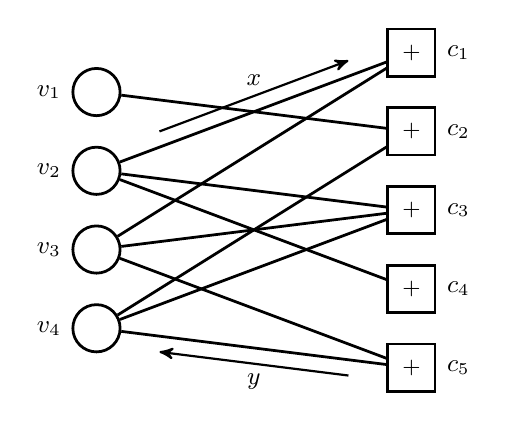
\begin{tikzpicture}
  [
  font=\small,
  line width=1pt,
  node distance = 3mm, draw=black, >=stealth',
  bitnode/.style={circle, inner sep = 0pt, minimum size = 6mm, draw=black},
  checknode/.style={rectangle, inner sep = 0pt, minimum size = 6mm, draw=black},
  ]

  \foreach \y in {1,2,3,4} {
    \node[bitnode] (b\y) at (0,0.5-\y) [label=left:$v_\y$]{};
  }
  
  \foreach \y in {1,2,3,4,5} {
    \node[checknode] (c\y) at (4,1-\y) [label=right:$c_\y$]{\footnotesize{$+$}};
  }

  \draw (b1) -- (c2);
  \draw (b2) -- (c1);
  \draw (b2) -- (c3);
  \draw (b2) -- (c4);
  \draw (b3) -- (c1);
  \draw (b3) -- (c3);
  \draw (b3) -- (c5);
  \draw (b4) -- (c2);
  \draw (b4) -- (c3);
  \draw (b4) -- (c5);

%  \draw[thick] (0,-1.5) -- (4,0);
%  \draw[thick] (0.8,-1.2) -- (3.2,-0.3);
  \draw[->,thick] (0.8,-1) -- node[above] {$x$} (3.2,-0.1);

%  \draw[thick] (0,-3.5) -- (4,-4);
%  \draw[thick] (0.8,-3.6) -- (3.2,-3.9);
  \draw[<-,thick] (0.8,-3.8) -- node[below] {$y$} (3.2,-4.1);

\end{tikzpicture}
}
  \end{center}
\column{.5\textwidth}
  \begin{center}
  \scalebox{0.7}{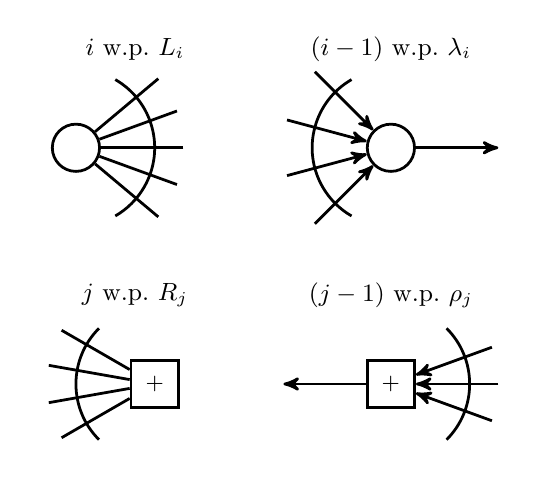
\begin{tikzpicture}
  [
  font=\small, line width=1pt, draw=black, >=stealth',
  bitnode/.style={circle, inner sep = 0pt, minimum size = 6mm, draw=black},
  checknode/.style={rectangle, inner sep = 0pt, minimum size = 6mm, draw=black},
  ]

  \node[bitnode] (L) at (0,3) {};
  \node[rotate around={-40:(L)}] (L0) at (1.5,3) {} edge (L);
  \node[rotate around={-20:(L)}] (L1) at (1.5,3) {} edge (L);
  \node[rotate around={0:(L)}] (L2) at (1.5,3) {} edge (L);
  \node[rotate around={20:(L)}] (L3) at (1.5,3) {} edge (L);
  \node[rotate around={40:(L)}] (L4) at (1.5,3) {} edge (L);
  \draw (L) ++(60:1) arc (60:-60:1);
  \node (Li) at (0.75,4.25) {$i$ w.p.\ $L_i$};

  \node[bitnode] (lambda) at (4,3) {};
  \node (lambda0) at (5.5,3) {} edge[<-] (lambda);
  \node[rotate around={-45:(lambda)}] (lambda1) at (2.5,3) {} edge[->] (lambda);
  \node[rotate around={-15:(lambda)}] (lambda2) at (2.5,3) {} edge[->] (lambda);
  \node[rotate around={15:(lambda)}] (lambda3) at (2.5,3) {} edge[->] (lambda);
  \node[rotate around={45:(lambda)}] (lambda4) at (2.5,3) {} edge[->] (lambda);
  \draw (lambda) ++(120:1) arc (120:240:1);
  \node (lambdai) at (4,4.25) {$(i-1)$ w.p.\ $\lambda_i$};
  
  \node[checknode] (R) at (1,0) {\footnotesize{$+$}};
  \node[rotate around={-30:(R)}] (R0) at (-0.5,0) {} edge (R);
  \node[rotate around={-10:(R)}] (R1) at (-0.5,0) {} edge (R);
  \node[rotate around={10:(R)}] (R2) at (-0.5,0) {} edge (R);
  \node[rotate around={30:(R)}] (R3) at (-0.5,0) {} edge (R);
  \draw (R) ++(135:1) arc (135:225:1);
  \node (Ri) at (0.75,1.125) {$j$ w.p.\ $R_j$};

  \node[checknode] (rho) at (4,0) {\footnotesize{$+$}};
  \node (R0) at (2.5,0) {} edge[<-] (rho);
  \node[rotate around={-20:(rho)}] (rho1) at (5.5,0) {} edge[->] (rho);
  \node (rho2) at (5.5,0) {} edge[->] (rho);
  \node[rotate around={20:(rho)}] (rho3) at (5.5,0) {} edge[->] (rho);
  \draw (rho) ++(45:1) arc (45:-45:1);
  \node (rhoi) at (4,1.125) {$(j-1)$ w.p.\ $\rho_j$};

\end{tikzpicture}
}
  \end{center}
\end{columns}
\myfootnote{\tiny
V. Zyablov, and M. Pinsker. \emph{Decoding complexity of low-density codes for transmission in a channel with erasures.} Problemy Peredachi Informatsii, 1974}
\myfootnote{\tiny
M. Luby, M. Mitzenmacher, A. Shokrollahi, and D. Spielman. \emph{Efficient erasure correcting codes}. IEEE Trans on Info Theory, 2001}
\end{frame}


\begin{frame}
\frametitle{Graphical Methods: Tools from Iterative Decoding}

\begin{itemize}
\item $x$: Prob.\ outgoing message from variable node erased
\item $y$: Prob.\ outgoing message from check node erased
\end{itemize}
\begin{center}
\scalebox{0.7}{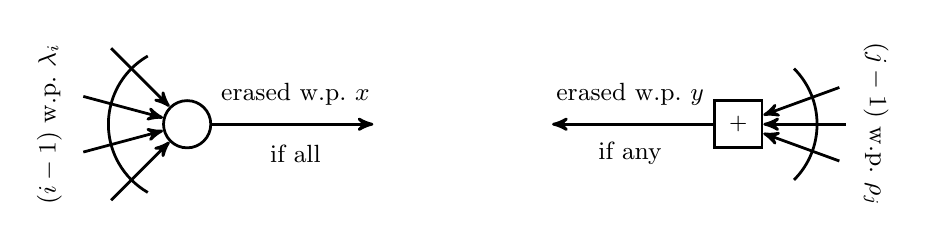
\begin{tikzpicture}
  [
  font=\small, line width=1pt, draw=black, >=stealth',
  bitnode/.style={circle, inner sep = 0pt, minimum size = 6mm, draw=black},
  checknode/.style={rectangle, inner sep = 0pt, minimum size = 6mm, draw=black},
  ]

  \node[bitnode] (lambda) at (0,0) {};
  \node (lambda0) at (2.5,0) {} edge[<-] (lambda);
  \node[rotate around={-45:(lambda)}] (lambda1) at (-1.5,0) {} edge[->] (lambda);
  \node[rotate around={-15:(lambda)}] (lambda2) at (-1.5,0) {} edge[->] (lambda);
  \node[rotate around={15:(lambda)}] (lambda3) at (-1.5,0) {} edge[->] (lambda);
  \node[rotate around={45:(lambda)}] (lambda4) at (-1.5,0) {} edge[->] (lambda);
  \draw (lambda) ++(120:1) arc (120:240:1);
  \node[rotate=90] (lambdai) at (-1.75,0) {$(i-1)$ w.p.\ $\lambda_i$};
  \node (x) at (1.375,0.375) {erased w.p.\ $x$};
  \node (x1) at (1.375,-0.375) {if all};
  
  \node[checknode] (rho) at (7,0) {\footnotesize{$+$}};
  \node (R0) at (4.5,0) {} edge[<-] (rho);
  \node[rotate around={-20:(rho)}] (rho1) at (8.5,0) {} edge[->] (rho);
  \node (rho2) at (8.5,0) {} edge[->] (rho);
  \node[rotate around={20:(rho)}] (rho3) at (8.5,0) {} edge[->] (rho);
  \draw (rho) ++(45:1) arc (45:-45:1);
  \node[rotate=-90] (rhoi) at (8.75,0) {$(j-1)$ w.p.\ $\rho_j$};
  \node (y) at (5.625,0.375) {erased w.p.\ $y$};
  \node (y1) at (5.625,-0.375) {if any};
\end{tikzpicture}
}
\end{center}
\begin{itemize}
\item Outgoing variable message is erased when all incoming check messages are erased
\begin{equation*}
x = \mathrm{E} \left[ y^{i-1} \right] = \lambda (y)
\end{equation*}
\item Outgoing check message is erased when one incoming variable message is erased
\begin{equation*}
y = \mathrm{E} \left[ 1 - (1 - x)^{j-1} \right] = 1 - \rho(1-x)
\end{equation*}
\end{itemize}
\end{frame}


\begin{frame}
\frametitle{Extrinsic Information Transfer (EXIT) Chart}
\begin{columns}
\column{.65\textwidth}
  \scalebox{0.85}{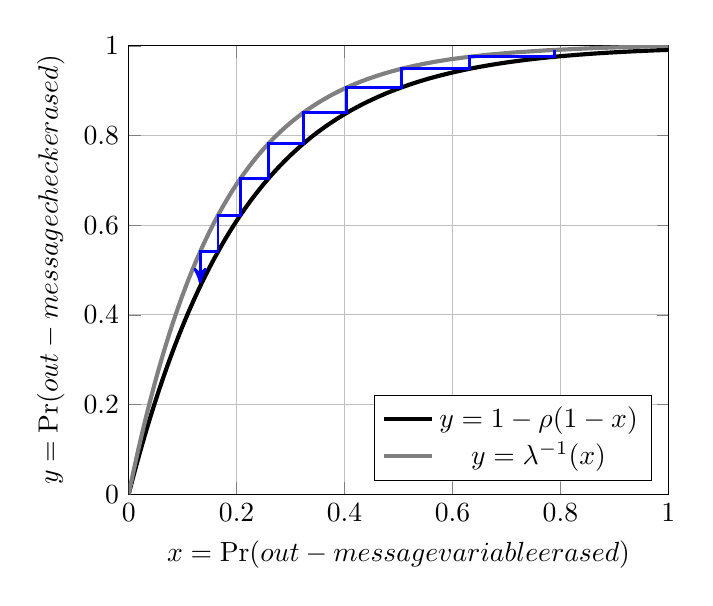
\begin{tikzpicture}
\begin{axis}[
  xlabel={$x = \Pr(\text{out-message variable erased})$},
  xmin=0, xmax=1,
  ymin=0, ymax=1,
  xmajorgrids,
  ylabel={$y = \Pr(\text{out-message check erased})$},
  legend pos=south east,
  ymajorgrids]

\addplot[color=black,line width=1.5pt]
coordinates{
(0.0000, 0.0000) (0.0050, 0.0232) (0.0100, 0.0459) (0.0150, 0.0681) (0.0200, 0.0898) (0.0250, 0.1109) (0.0300, 0.1316) (0.0350, 0.1518) (0.0400, 0.1715) (0.0450, 0.1907) (0.0500, 0.2095) (0.0550, 0.2279) (0.0600, 0.2458) (0.0650, 0.2634) (0.0700, 0.2805) (0.0750, 0.2972) (0.0800, 0.3135) (0.0850, 0.3295) (0.0900, 0.3451) (0.0950, 0.3603) (0.1000, 0.3751) (0.1050, 0.3897) (0.1100, 0.4039) (0.1150, 0.4177) (0.1200, 0.4312) (0.1250, 0.4445) (0.1300, 0.4574) (0.1350, 0.4700) (0.1400, 0.4823) (0.1450, 0.4943) (0.1500, 0.5061) (0.1550, 0.5175) (0.1600, 0.5288) (0.1650, 0.5397) (0.1700, 0.5504) (0.1750, 0.5609) (0.1800, 0.5711) (0.1850, 0.5810) (0.1900, 0.5908) (0.1950, 0.6003) (0.2000, 0.6096) (0.2050, 0.6186) (0.2100, 0.6275) (0.2150, 0.6362) (0.2200, 0.6446) (0.2250, 0.6529) (0.2300, 0.6609) (0.2350, 0.6688) (0.2400, 0.6765) (0.2450, 0.6840) (0.2500, 0.6914) (0.2550, 0.6985) (0.2600, 0.7055) (0.2650, 0.7124) (0.2700, 0.7191) (0.2750, 0.7256) (0.2800, 0.7320) (0.2850, 0.7382) (0.2900, 0.7443) (0.2950, 0.7502) (0.3000, 0.7560) (0.3050, 0.7617) (0.3100, 0.7672) (0.3150, 0.7726) (0.3200, 0.7779) (0.3250, 0.7831) (0.3300, 0.7881) (0.3350, 0.7931) (0.3400, 0.7979) (0.3450, 0.8026) (0.3500, 0.8072) (0.3550, 0.8116) (0.3600, 0.8160) (0.3650, 0.8203) (0.3700, 0.8245) (0.3750, 0.8285) (0.3800, 0.8325) (0.3850, 0.8364) (0.3900, 0.8402) (0.3950, 0.8439) (0.4000, 0.8476) (0.4050, 0.8511) (0.4100, 0.8546) (0.4150, 0.8579) (0.4200, 0.8612) (0.4250, 0.8645) (0.4300, 0.8676) (0.4350, 0.8707) (0.4400, 0.8737) (0.4450, 0.8766) (0.4500, 0.8795) (0.4550, 0.8823) (0.4600, 0.8850) (0.4650, 0.8877) (0.4700, 0.8903) (0.4750, 0.8929) (0.4800, 0.8954) (0.4850, 0.8978) (0.4900, 0.9002) (0.4950, 0.9025) (0.5000, 0.9047) (0.5050, 0.9070) (0.5100, 0.9091) (0.5150, 0.9112) (0.5200, 0.9133) (0.5250, 0.9153) (0.5300, 0.9173) (0.5350, 0.9192) (0.5400, 0.9211) (0.5450, 0.9229) (0.5500, 0.9247) (0.5550, 0.9265) (0.5600, 0.9282) (0.5650, 0.9298) (0.5700, 0.9315) (0.5750, 0.9331) (0.5800, 0.9346) (0.5850, 0.9361) (0.5900, 0.9376) (0.5950, 0.9391) (0.6000, 0.9405) (0.6050, 0.9419) (0.6100, 0.9432) (0.6150, 0.9445) (0.6200, 0.9458) (0.6250, 0.9471) (0.6300, 0.9483) (0.6350, 0.9495) (0.6400, 0.9507) (0.6450, 0.9518) (0.6500, 0.9530) (0.6550, 0.9540) (0.6600, 0.9551) (0.6650, 0.9562) (0.6700, 0.9572) (0.6750, 0.9582) (0.6800, 0.9591) (0.6850, 0.9601) (0.6900, 0.9610) (0.6950, 0.9619) (0.7000, 0.9628) (0.7050, 0.9637) (0.7100, 0.9645) (0.7150, 0.9653) (0.7200, 0.9661) (0.7250, 0.9669) (0.7300, 0.9677) (0.7350, 0.9685) (0.7400, 0.9692) (0.7450, 0.9699) (0.7500, 0.9706) (0.7550, 0.9713) (0.7600, 0.9720) (0.7650, 0.9726) (0.7700, 0.9732) (0.7750, 0.9739) (0.7800, 0.9745) (0.7850, 0.9751) (0.7900, 0.9756) (0.7950, 0.9762) (0.8000, 0.9768) (0.8050, 0.9773) (0.8100, 0.9778) (0.8150, 0.9783) (0.8200, 0.9788) (0.8250, 0.9793) (0.8300, 0.9798) (0.8350, 0.9803) (0.8400, 0.9807) (0.8450, 0.9812) (0.8500, 0.9816) (0.8550, 0.9821) (0.8600, 0.9825) (0.8650, 0.9829) (0.8700, 0.9833) (0.8750, 0.9837) (0.8800, 0.9840) (0.8850, 0.9844) (0.8900, 0.9848) (0.8950, 0.9851) (0.9000, 0.9855) (0.9050, 0.9858) (0.9100, 0.9861) (0.9150, 0.9865) (0.9200, 0.9868) (0.9250, 0.9871) (0.9300, 0.9874) (0.9350, 0.9877) (0.9400, 0.9880) (0.9450, 0.9882) (0.9500, 0.9885) (0.9550, 0.9888) (0.9600, 0.9890) (0.9650, 0.9893) (0.9700, 0.9896) (0.9750, 0.9898) (0.9800, 0.9900) (0.9850, 0.9903) (0.9900, 0.9905) (0.9950, 0.9907) (1.0000, 0.9909)
};
\addlegendentry{$y = 1 - \rho (1 - x)$}

\addplot[color=gray,line width=1.5pt]
coordinates{
(0.0000, 0.0000) (0.0009, 0.0050) (0.0017, 0.0100) (0.0026, 0.0150) (0.0034, 0.0200) (0.0043, 0.0250) (0.0052, 0.0300) (0.0061, 0.0350) (0.0069, 0.0400) (0.0078, 0.0450) (0.0087, 0.0500) (0.0096, 0.0550) (0.0105, 0.0600) (0.0114, 0.0650) (0.0123, 0.0700) (0.0133, 0.0750) (0.0142, 0.0800) (0.0151, 0.0850) (0.0160, 0.0900) (0.0170, 0.0950) (0.0179, 0.1000) (0.0189, 0.1050) (0.0198, 0.1100) (0.0208, 0.1150) (0.0217, 0.1200) (0.0227, 0.1250) (0.0237, 0.1300) (0.0247, 0.1350) (0.0257, 0.1400) (0.0267, 0.1450) (0.0276, 0.1500) (0.0287, 0.1550) (0.0297, 0.1600) (0.0307, 0.1650) (0.0317, 0.1700) (0.0327, 0.1750) (0.0338, 0.1800) (0.0348, 0.1850) (0.0358, 0.1900) (0.0369, 0.1950) (0.0380, 0.2000) (0.0390, 0.2050) (0.0401, 0.2100) (0.0412, 0.2150) (0.0423, 0.2200) (0.0434, 0.2250) (0.0445, 0.2300) (0.0456, 0.2350) (0.0467, 0.2400) (0.0478, 0.2450) (0.0489, 0.2500) (0.0501, 0.2550) (0.0512, 0.2600) (0.0524, 0.2650) (0.0535, 0.2700) (0.0547, 0.2750) (0.0559, 0.2800) (0.0571, 0.2850) (0.0583, 0.2900) (0.0595, 0.2950) (0.0607, 0.3000) (0.0619, 0.3050) (0.0631, 0.3100) (0.0644, 0.3150) (0.0656, 0.3200) (0.0669, 0.3250) (0.0681, 0.3300) (0.0694, 0.3350) (0.0707, 0.3400) (0.0720, 0.3450) (0.0733, 0.3500) (0.0746, 0.3550) (0.0759, 0.3600) (0.0773, 0.3650) (0.0786, 0.3700) (0.0800, 0.3750) (0.0813, 0.3800) (0.0827, 0.3850) (0.0841, 0.3900) (0.0855, 0.3950) (0.0869, 0.4000) (0.0883, 0.4050) (0.0898, 0.4100) (0.0912, 0.4150) (0.0927, 0.4200) (0.0941, 0.4250) (0.0956, 0.4300) (0.0971, 0.4350) (0.0986, 0.4400) (0.1002, 0.4450) (0.1017, 0.4500) (0.1033, 0.4550) (0.1048, 0.4600) (0.1064, 0.4650) (0.1080, 0.4700) (0.1096, 0.4750) (0.1112, 0.4800) (0.1129, 0.4850) (0.1146, 0.4900) (0.1162, 0.4950) (0.1179, 0.5000) (0.1196, 0.5050) (0.1214, 0.5100) (0.1231, 0.5150) (0.1249, 0.5200) (0.1266, 0.5250) (0.1284, 0.5300) (0.1303, 0.5350) (0.1321, 0.5400) (0.1340, 0.5450) (0.1358, 0.5500) (0.1377, 0.5550) (0.1397, 0.5600) (0.1416, 0.5650) (0.1436, 0.5700) (0.1456, 0.5750) (0.1476, 0.5800) (0.1496, 0.5850) (0.1517, 0.5900) (0.1538, 0.5950) (0.1559, 0.6000) (0.1580, 0.6050) (0.1602, 0.6100) (0.1624, 0.6150) (0.1646, 0.6200) (0.1669, 0.6250) (0.1691, 0.6300) (0.1715, 0.6350) (0.1738, 0.6400) (0.1762, 0.6450) (0.1786, 0.6500) (0.1810, 0.6550) (0.1835, 0.6600) (0.1861, 0.6650) (0.1886, 0.6700) (0.1912, 0.6750) (0.1938, 0.6800) (0.1965, 0.6850) (0.1992, 0.6900) (0.2020, 0.6950) (0.2048, 0.7000) (0.2077, 0.7050) (0.2106, 0.7100) (0.2136, 0.7150) (0.2166, 0.7200) (0.2196, 0.7250) (0.2228, 0.7300) (0.2259, 0.7350) (0.2292, 0.7400) (0.2325, 0.7450) (0.2358, 0.7500) (0.2393, 0.7550) (0.2428, 0.7600) (0.2464, 0.7650) (0.2500, 0.7700) (0.2538, 0.7750) (0.2576, 0.7800) (0.2615, 0.7850) (0.2655, 0.7900) (0.2696, 0.7950) (0.2738, 0.8000) (0.2781, 0.8050) (0.2825, 0.8100) (0.2871, 0.8150) (0.2917, 0.8200) (0.2965, 0.8250) (0.3015, 0.8300) (0.3065, 0.8350) (0.3118, 0.8400) (0.3172, 0.8450) (0.3227, 0.8500) (0.3285, 0.8550) (0.3345, 0.8600) (0.3407, 0.8650) (0.3471, 0.8700) (0.3538, 0.8750) (0.3607, 0.8800) (0.3680, 0.8850) (0.3755, 0.8900) (0.3834, 0.8950) (0.3917, 0.9000) (0.4005, 0.9050) (0.4097, 0.9100) (0.4194, 0.9150) (0.4297, 0.9200) (0.4407, 0.9250) (0.4524, 0.9300) (0.4650, 0.9350) (0.4786, 0.9400) (0.4934, 0.9450) (0.5096, 0.9500) (0.5276, 0.9550) (0.5476, 0.9600) (0.5703, 0.9650) (0.5965, 0.9700) (0.6274, 0.9750) (0.6649, 0.9800) (0.7123, 0.9850) (0.7753, 0.9900) (0.8644, 0.9950) (1.0000, 1.0000)
};
\addlegendentry{$y = \lambda^{-1}(x)$}

\addplot[color=blue,line width=1pt,->,>=stealth']
coordinates{
(0.7894, 0.9909) (0.7894, 0.9756) (0.6313, 0.9756) (0.6313, 0.9486) (0.5051, 0.9486) (0.5051, 0.9070) (0.4040, 0.9070) (0.4040, 0.8504) (0.3232, 0.8504) (0.3232, 0.7813) (0.2586, 0.7813) (0.2586, 0.7036) (0.2069, 0.7036) (0.2069, 0.6220) (0.1655, 0.6220) (0.1655, 0.5408) (0.1324, 0.5408)
(0.1324, 0.47)
};
\end{axis}
\end{tikzpicture}
}
\column{.3\textwidth}
  \scalebox{0.85}{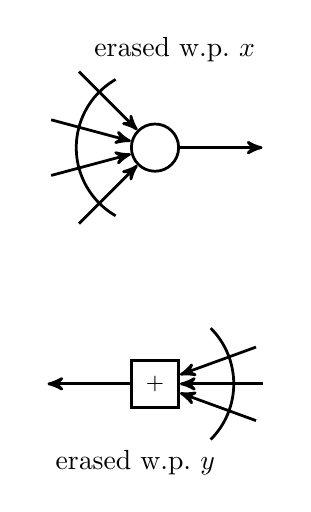
\begin{tikzpicture}
  [
  %font=\small,
  line width=1pt,
  draw=black, >=stealth',
  bitnode/.style={circle, inner sep = 0pt, minimum size = 6mm, draw=black},
  checknode/.style={rectangle, inner sep = 0pt, minimum size = 6mm, draw=black},
  ]

  \node[bitnode] (lambda) at (0,3) {};
  \node (lambda0) at (1.5,3) {} edge[<-] (lambda);
  \node[rotate around={-45:(lambda)}] (lambda1) at (-1.5,3) {} edge[->] (lambda);
  \node[rotate around={-15:(lambda)}] (lambda2) at (-1.5,3) {} edge[->] (lambda);
  \node[rotate around={15:(lambda)}] (lambda3) at (-1.5,3) {} edge[->] (lambda);
  \node[rotate around={45:(lambda)}] (lambda4) at (-1.5,3) {} edge[->] (lambda);
  \draw (lambda) ++(120:1) arc (120:240:1);
  \node (x) at (0.25,4.25) {erased w.p.\ $x$};
  
  \node[checknode] (rho) at (0,0) {\footnotesize{$+$}};
  \node (R0) at (-1.5,0) {} edge[<-] (rho);
  \node[rotate around={-20:(rho)}] (rho1) at (1.5,0) {} edge[->] (rho);
  \node (rho2) at (1.5,0) {} edge[->] (rho);
  \node[rotate around={20:(rho)}] (rho3) at (1.5,0) {} edge[->] (rho);
  \draw (rho) ++(45:1) arc (45:-45:1);
  \node (x) at (-0.25,-1) {erased w.p.\ $y$};
\end{tikzpicture}

}
\end{columns}
\vfill
\textbf{Step-by-Step Progression}
\begin{xalignat*}{2}
y &= 1 - \rho(1-x) &
x &= \lambda(y) \quad \text{ \textcolor{gray}{(flipped)}}
\end{xalignat*}
\end{frame}


\begin{frame}
\frametitle{Unsourced MAC -- SIC UGMAC Scheme}
\begin{center}
\scalebox{0.75}{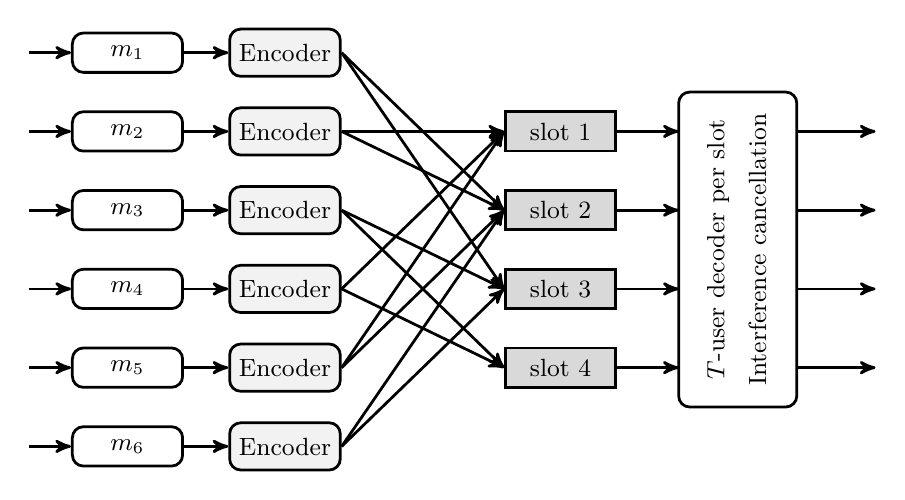
\begin{tikzpicture}
  [
  font=\small, line width=1pt, draw=black, >=stealth',
  slot/.style={rectangle, minimum height=5mm, minimum width=14mm, draw=black, fill=gray!30},
  encoder/.style={rectangle, minimum height=6mm, minimum width=14mm, draw=black, fill=gray!10, rounded corners},
  decoder/.style={rectangle, minimum height=6mm, minimum width=14mm, draw=black, rounded corners},
  message/.style={rectangle, minimum height=5mm, minimum width=14mm, draw=black, rounded corners}
  ]

\foreach \e in {1,2,3,4,5,6} {
  \node[encoder] (e\e) at (2,0.5-\e) {Encoder};
}

\foreach \m in {1,2,3,4,5,6} {
  \node[message] (m\m) at (0,0.5-\m) {$m_{\m}$}
  edge[->] (e\m);
  \draw[<-] (m\m) -- (-1.25,0.5-\m);
}
  
\foreach \s in {1,2,3,4} {
  \node[slot] (c\s) at (5.5,-0.5-\s) {slot~\s};
  %\node[decoder] (d\s) at (8,-0.5-\s) {Decoder};
  \draw[->] (c\s) -- (7,-0.5-\s);
}

\draw[rounded corners] (7,-1) rectangle (8.5,-5);
\node[rotate=90] (d1) at (7.5,-3) {$T$-user decoder per slot};
\node[rotate=90] (d2) at (8,-3) {Interference cancellation};

\draw[->] (8.5,-1.5) -- (9.5,-1.5);
\draw[->] (8.5,-2.5) -- (9.5,-2.5);
\draw[->] (8.5,-3.5) -- (9.5,-3.5);
\draw[->] (8.5,-4.5) -- (9.5,-4.5);

\draw[->] (e1.east) -- (c2.west);
\draw[->] (e2.east) -- (c1.west);
\draw[->] (e3.east) -- (c3.west);
\draw[->] (e4.east) -- (c4.west);
\draw[->] (e5.east) -- (c1.west);
\draw[->] (e6.east) -- (c3.west);
\draw[->] (e1.east) -- (c3.west);
\draw[->] (e2.east) -- (c2.west);
\draw[->] (e3.east) -- (c4.west);
\draw[->] (e4.east) -- (c1.west);
\draw[->] (e5.east) -- (c2.west);
\draw[->] (e6.east) -- (c2.west);
\end{tikzpicture}
}
\end{center}
\begin{block}{Key Features}
\begin{itemize}
\item Schedule selected based on \textbf{message bits}
\item Devices can transmit in multiple sub-blocks
\item Scheme facilitates peeling decoder
\end{itemize}
\end{block}
\myfootnote{\tiny
A. Vem, K. Narayanan, J. Cheng, JFC.
\emph{A User-Independent Successive Interference Cancellation Based Coding Scheme for the Unsourced Random Access Gaussian Channel}.
IEEE Trans on Comm, 2019}
\end{frame}


\begin{frame}
\frametitle{What Really Happens within Slot?}
\begin{center}
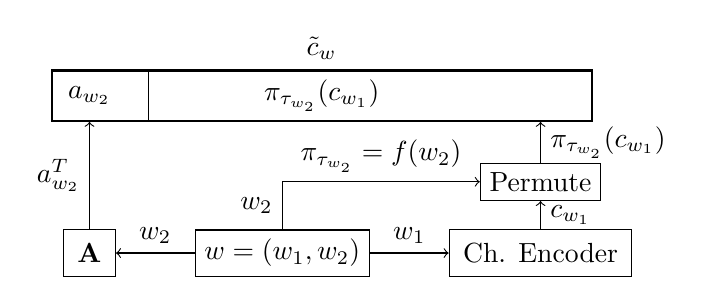
\begin{tikzpicture}

%Message node and final codeword Rectangle
\node[draw,rectangle] (msg) at (3,1) {$w=(w_1,w_2)$};
\node[rectangle, draw, minimum width=2.7in,thick] (codeword) at (3.5,3) {$\pi_{\tau_{w_2}}({c}_{w_1})$}; 
%$c_{w}(\pi_{\tau_{w_2}^1}),c_{w}(\pi_{\tau_{w_2}^2}),\ldots,c_{w}(\pi_{\tau_{w_2}})$};


% From messages to Ch. Encoder and Compressive Sensing Encoder
\draw [->] (msg.east) -- +(0:1) node[midway, above] {$w_1$} node[draw, inner sep=5pt,at end, anchor= west] (encoder) {Ch. Encoder} ;
\draw [->] (msg.west) -- +(0:-1) node[midway, above] {$w_2$} node[draw, inner sep=5pt,at end, anchor= east] (CSencoder) {$\mathbf{A}$}; %{Sensing Matrix $\mathbf{A}$};

\path (encoder.north)-- +(90:0.6) node[draw, rectangle,fill=white](CWperm){Permute};
\draw[->] (encoder.north)-- (CWperm.south) node[midway,right]{${c}_{w_1}$};
\draw[->](CWperm.north)-- (CWperm.north |- codeword.south) node[midway, right]{$\pi_{\tau_{w_2}}({c}_{w_1})$};

\draw[->](CSencoder.north)-- (CSencoder.north |- codeword.south) node[midway, left]{${a}^T_{w_2}$};

\path let \p{A}=(codeword) in (3-1.7,\y{A})node (partition){} -- (partition |- codeword.north);
\draw (partition |- codeword.north) -- (partition |- codeword.south) ;
\node () at (partition -| CSencoder) {${a}_{w_2}$};
\node [above] at (codeword.north) {${\tilde{c}}_{w}$};

\draw [->] (msg.north) -- (msg.north |- CWperm.west)node[midway,left]{$w_2$} -- (CWperm.west) node[midway,above] {$\pi_{\tau_{w_2}}=f(w_2)$};
\end{tikzpicture}

\end{center}
\begin{block}{Implementation Notes}
  \begin{itemize}
\item Message is partitioned into two parts $w = (w_1, w_2)$
  \item Every device uses identical codebook built from spatially-coupled LDPC-type codes tailored to $T$-user real-adder channel
  \item $w_2$ dictate permutation on encoder and recovered through CS
  \item Non-negative $\ell_1$-regularized LASSO
  %\item MMSE estimator on list
  \end{itemize}
\end{block}
\myfootnote{\tiny
A. Vem, K. Narayanan, J. Cheng, JFC.
\emph{A User-Independent Successive Interference Cancellation Based Coding Scheme for the Unsourced Random Access Gaussian Channel}.
IEEE Trans on Comm, 2019}
\end{frame}


\begin{frame}
\frametitle{Limitations of Sparsifying Collisions}
\begin{columns}
\column{.5\textwidth}
\begin{block}{Drawbacks of Slots}
  \begin{itemize}
  \item Stochastic binning and expectation of concave rewards
  \item Second order dispersion effects comes into play in FBL
  \item Energy expended solely to resolving collisions
  \item Gray slots are discarded during decoding process (60\%)
  \end{itemize}
\end{block}
\column{.45\textwidth}
  \centerline{\scalebox{0.42}{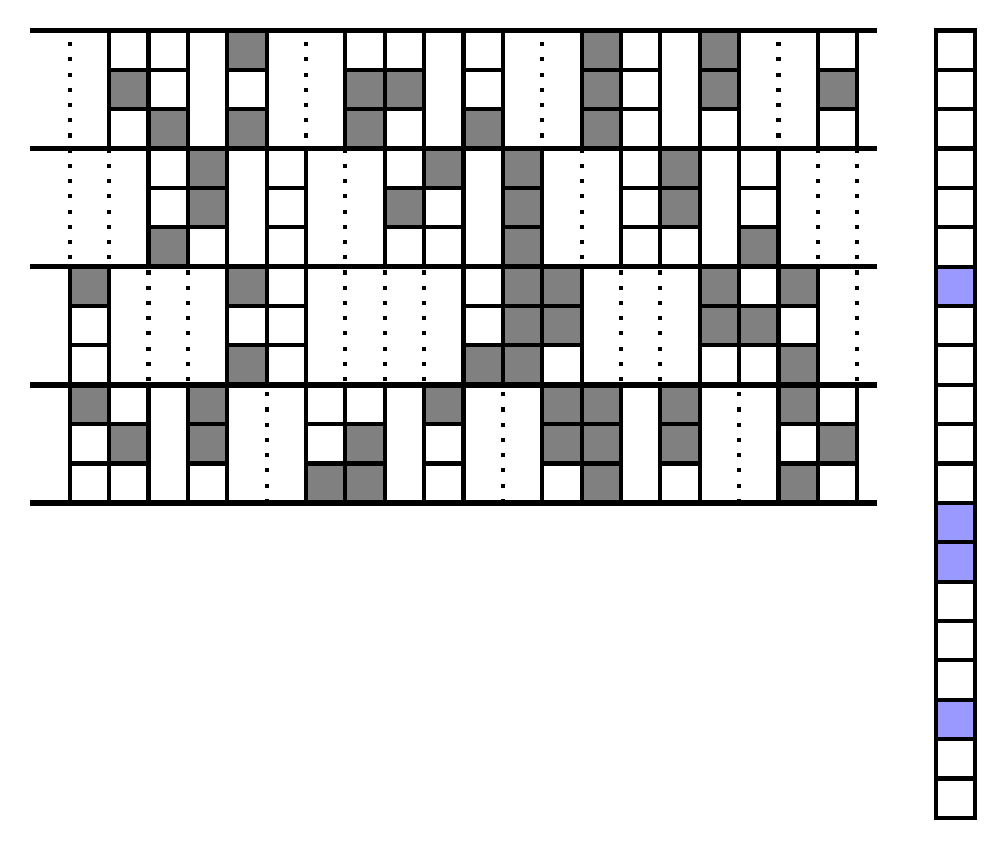
\begin{tikzpicture}
[draw=black, line width=1.5pt, >=stealth',
entry0/.style={rectangle, draw, inner sep=0pt, minimum size=5mm},
entry1/.style={rectangle, draw, fill=gray, inner sep=0pt, minimum size=5mm},
symbol0/.style={rectangle, draw, fill=white, inner sep=0pt, minimum size=5mm},
symbol/.style={rectangle, draw, fill=blue!40, inner sep=0pt, minimum size=5mm}]

\node[entry0] (m0000) at (0,0) {};
\node[entry0] (m0001) at (0.5,0) {};
%\node[entry1] (m0002) at (1,0) {};
\node[entry0] (m0003) at (1.5,0) {};
%\node[entry1] (m0004) at (2,0) {};
%\node[entry0] (m0005) at (2.5,0) {};
\node[entry1] (m0006) at (3,0) {};
\node[entry1] (m0007) at (3.5,0) {};
%\node[entry0] (m0008) at (4,0) {};
\node[entry0] (m0009) at (4.5,0) {};
%\node[entry1] (m0010) at (5,0) {};
%\node[entry1] (m0011) at (5.5,0) {};
\node[entry0] (m0012) at (6,0) {};
\node[entry1] (m0013) at (6.5,0) {};
%\node[entry0] (m0014) at (7,0) {};
\node[entry0] (m0015) at (7.5,0) {};
%\node[entry0] (m0016) at (8,0) {};
%\node[entry0] (m0017) at (8.5,0) {};
\node[entry1] (m0018) at (9,0) {};
\node[entry0] (m0019) at (9.5,0) {};

\node[entry0] (m0100) at (0,0.5) {};
\node[entry1] (m0101) at (0.5,0.5) {};
%\node[entry0] (m0102) at (1,0.5) {};
\node[entry1] (m0103) at (1.5,0.5) {};
%\node[entry0] (m0104) at (2,0.5) {};
%\node[entry0] (m0105) at (2.5,0.5) {};
\node[entry0] (m0106) at (3,0.5) {};
\node[entry1] (m0107) at (3.5,0.5) {};
%\node[entry1] (m0108) at (4,0.5) {};
\node[entry0] (m0109) at (4.5,0.5) {};
%\node[entry0] (m0110) at (5,0.5) {};
%\node[entry1] (m0111) at (5.5,0.5) {};
\node[entry1] (m0112) at (6,0.5) {};
\node[entry1] (m0113) at (6.5,0.5) {};
%\node[entry0] (m0114) at (7,0.5) {};
\node[entry1] (m0115) at (7.5,0.5) {};
%\node[entry1] (m0116) at (8,0.5) {};
%\node[entry0] (m0117) at (8.5,0.5) {};
\node[entry0] (m0118) at (9,0.5) {};
\node[entry1] (m0119) at (9.5,0.5) {};

\node[entry1] (m0200) at (0,1) {};
\node[entry0] (m0201) at (0.5,1) {};
%\node[entry0] (m0202) at (1,1) {};
\node[entry1] (m0203) at (1.5,1) {};
%\node[entry1] (m0204) at (2,1) {};
%\node[entry0] (m0205) at (2.5,1) {};
\node[entry0] (m0206) at (3,1) {};
\node[entry0] (m0207) at (3.5,1) {};
%\node[entry0] (m0208) at (4,1) {};
\node[entry1] (m0209) at (4.5,1) {};
%\node[entry0] (m0210) at (5,1) {};
%\node[entry1] (m0211) at (5.5,1) {};
\node[entry1] (m0212) at (6,1) {};
\node[entry1] (m0213) at (6.5,1) {};
%\node[entry0] (m0214) at (7,1) {};
\node[entry1] (m0215) at (7.5,1) {};
%\node[entry1] (m0216) at (8,1) {};
%\node[entry0] (m0217) at (8.5,1) {};
\node[entry1] (m0218) at (9,1) {};
\node[entry0] (m0219) at (9.5,1) {};

\node[entry0] (m0300) at (0,1.5) {};
%\node[entry0] (m0301) at (0.5,1.5) {};
%\node[entry1] (m0302) at (1,1.5) {};
%\node[entry0] (m0303) at (1.5,1.5) {};
\node[entry1] (m0304) at (2,1.5) {};
\node[entry0] (m0305) at (2.5,1.5) {};
%\node[entry1] (m0306) at (3,1.5) {};
%\node[entry1] (m0307) at (3.5,1.5) {};
%\node[entry0] (m0308) at (4,1.5) {};
%\node[entry0] (m0309) at (4.5,1.5) {};
\node[entry1] (m0310) at (5,1.5) {};
\node[entry1] (m0311) at (5.5,1.5) {};
\node[entry0] (m0312) at (6,1.5) {};
%\node[entry1] (m0313) at (6.5,1.5) {};
%\node[entry0] (m0314) at (7,1.5) {};
%\node[entry0] (m0315) at (7.5,1.5) {};
\node[entry0] (m0316) at (8,1.5) {};
\node[entry0] (m0317) at (8.5,1.5) {};
\node[entry1] (m0318) at (9,1.5) {};
%\node[entry0] (m0319) at (9.5,1.5) {};

\node[entry0] (m0400) at (0,2) {};
%\node[entry1] (m0401) at (0.5,2) {};
%\node[entry0] (m0402) at (1,2) {};
%\node[entry1] (m0403) at (1.5,2) {};
\node[entry0] (m0404) at (2,2) {};
\node[entry0] (m0405) at (2.5,2) {};
%\node[entry0] (m0406) at (3,2) {};
%\node[entry1] (m0407) at (3.5,2) {};
%\node[entry1] (m0408) at (4,2) {};
%\node[entry0] (m0409) at (4.5,2) {};
\node[entry0] (m0410) at (5,2) {};
\node[entry1] (m0411) at (5.5,2) {};
\node[entry1] (m0412) at (6,2) {};
%\node[entry1] (m0413) at (6.5,2) {};
%\node[entry0] (m0414) at (7,2) {};
%\node[entry1] (m0415) at (7.5,2) {};
\node[entry1] (m0416) at (8,2) {};
\node[entry1] (m0417) at (8.5,2) {};
\node[entry0] (m0418) at (9,2) {};
%\node[entry1] (m0419) at (9.5,2) {};

\node[entry1] (m0500) at (0,2.5) {};
%\node[entry0] (m0501) at (0.5,2.5) {};
%\node[entry0] (m0502) at (1,2.5) {};
%\node[entry1] (m0503) at (1.5,2.5) {};
\node[entry1] (m0504) at (2,2.5) {};
\node[entry0] (m0505) at (2.5,2.5) {};
%\node[entry0] (m0506) at (3,2.5) {};
%\node[entry0] (m0507) at (3.5,2.5) {};
%\node[entry0] (m0508) at (4,2.5) {};
%\node[entry1] (m0509) at (4.5,2.5) {};
\node[entry0] (m0510) at (5,2.5) {};
\node[entry1] (m0511) at (5.5,2.5) {};
\node[entry1] (m0512) at (6,2.5) {};
%\node[entry1] (m0513) at (6.5,2.5) {};
%\node[entry0] (m0514) at (7,2.5) {};
%\node[entry1] (m0515) at (7.5,2.5) {};
\node[entry1] (m0516) at (8,2.5) {};
\node[entry0] (m0517) at (8.5,2.5) {};
\node[entry1] (m0518) at (9,2.5) {};
%\node[entry0] (m0519) at (9.5,2.5) {};

%\node[entry0] (m0600) at (0,3) {};
%\node[entry0] (m0601) at (0.5,3) {};
\node[entry1] (m0602) at (1,3) {};
\node[entry0] (m0603) at (1.5,3) {};
%\node[entry1] (m0604) at (2,3) {};
\node[entry0] (m0605) at (2.5,3) {};
%\node[entry1] (m0606) at (3,3) {};
%\node[entry1] (m0607) at (3.5,3) {};
\node[entry0] (m0608) at (4,3) {};
\node[entry0] (m0609) at (4.5,3) {};
%\node[entry1] (m0610) at (5,3) {};
\node[entry1] (m0611) at (5.5,3) {};
%\node[entry0] (m0612) at (6,3) {};
%\node[entry1] (m0613) at (6.5,3) {};
\node[entry0] (m0614) at (7,3) {};
\node[entry0] (m0615) at (7.5,3) {};
%\node[entry0] (m0616) at (8,3) {};
\node[entry1] (m0617) at (8.5,3) {};
%\node[entry1] (m0618) at (9,3) {};
%\node[entry0] (m0619) at (9.5,3) {};

%\node[entry0] (m0700) at (0,3.5) {};
%\node[entry1] (m0701) at (0.5,3.5) {};
\node[entry0] (m0702) at (1,3.5) {};
\node[entry1] (m0703) at (1.5,3.5) {};
%\node[entry0] (m0704) at (2,3.5) {};
\node[entry0] (m0705) at (2.5,3.5) {};
%\node[entry0] (m0706) at (3,3.5) {};
%\node[entry1] (m0707) at (3.5,3.5) {};
\node[entry1] (m0708) at (4,3.5) {};
\node[entry0] (m0709) at (4.5,3.5) {};
%\node[entry0] (m0710) at (5,3.5) {};
\node[entry1] (m0711) at (5.5,3.5) {};
%\node[entry1] (m0712) at (6,3.5) {};
%\node[entry1] (m0713) at (6.5,3.5) {};
\node[entry0] (m0714) at (7,3.5) {};
\node[entry1] (m0715) at (7.5,3.5) {};
%\node[entry1] (m0716) at (8,3.5) {};
\node[entry0] (m0717) at (8.5,3.5) {};
%\node[entry1] (m0718) at (9,3.5) {};
%\node[entry1] (m0719) at (9.5,3.5) {};

%\node[entry1] (m0800) at (0,4) {};
%\node[entry0] (m0801) at (0.5,4) {};
\node[entry0] (m0802) at (1,4) {};
\node[entry1] (m0803) at (1.5,4) {};
%\node[entry1] (m0804) at (2,4) {};
\node[entry0] (m0805) at (2.5,4) {};
%\node[entry0] (m0806) at (3,4) {};
%\node[entry0] (m0807) at (3.5,4) {};
\node[entry0] (m0808) at (4,4) {};
\node[entry1] (m0809) at (4.5,4) {};
%\node[entry0] (m0810) at (5,4) {};
\node[entry1] (m0811) at (5.5,4) {};
%\node[entry1] (m0812) at (6,4) {};
%\node[entry1] (m0813) at (6.5,4) {};
\node[entry0] (m0814) at (7,4) {};
\node[entry1] (m0815) at (7.5,4) {};
%\node[entry1] (m0816) at (8,4) {};
\node[entry0] (m0817) at (8.5,4) {};
%\node[entry1] (m0818) at (9,4) {};
%\node[entry0] (m0819) at (9.5,4) {};

%\node[entry0] (m0900) at (0,4.5) {};
\node[entry0] (m0901) at (0.5,4.5) {};
\node[entry1] (m0902) at (1,4.5) {};
%\node[entry0] (m0903) at (1.5,4.5) {};
\node[entry1] (m0904) at (2,4.5) {};
%\node[entry0] (m0905) at (2.5,4.5) {};
%\node[entry1] (m0906) at (3,4.5) {};
\node[entry1] (m0907) at (3.5,4.5) {};
\node[entry0] (m0908) at (4,4.5) {};
%\node[entry0] (m0909) at (4.5,4.5) {};
\node[entry1] (m0910) at (5,4.5) {};
%\node[entry1] (m0911) at (5.5,4.5) {};
%\node[entry0] (m0912) at (6,4.5) {};
\node[entry1] (m0913) at (6.5,4.5) {};
\node[entry0] (m0914) at (7,4.5) {};
%\node[entry0] (m0915) at (7.5,4.5) {};
\node[entry0] (m0916) at (8,4.5) {};
%\node[entry0] (m0917) at (8.5,4.5) {};
%\node[entry1] (m0918) at (9,4.5) {};
\node[entry0] (m0919) at (9.5,4.5) {};

%\node[entry0] (m1000) at (0,5) {};
\node[entry1] (m1001) at (0.5,5) {};
\node[entry0] (m1002) at (1,5) {};
%\node[entry1] (m1003) at (1.5,5) {};
\node[entry0] (m1004) at (2,5) {};
%\node[entry0] (m1005) at (2.5,5) {};
%\node[entry0] (m1006) at (3,5) {};
\node[entry1] (m1007) at (3.5,5) {};
\node[entry1] (m1008) at (4,5) {};
%\node[entry0] (m1009) at (4.5,5) {};
\node[entry0] (m1010) at (5,5) {};
%\node[entry1] (m1011) at (5.5,5) {};
%\node[entry1] (m1012) at (6,5) {};
\node[entry1] (m1013) at (6.5,5) {};
\node[entry0] (m1014) at (7,5) {};
%\node[entry1] (m1015) at (7.5,5) {};
\node[entry1] (m1016) at (8,5) {};
%\node[entry0] (m1017) at (8.5,5) {};
%\node[entry0] (m1018) at (9,5) {};
\node[entry1] (m1019) at (9.5,5) {};

%\node[entry1] (m1100) at (0,5.5) {};
\node[entry0] (m1101) at (0.5,5.5) {};
\node[entry0] (m1102) at (1,5.5) {};
%\node[entry1] (m1103) at (1.5,5.5) {};
\node[entry1] (m1104) at (2,5.5) {};
%\node[entry0] (m1105) at (2.5,5.5) {};
%\node[entry0] (m1106) at (3,5.5) {};
\node[entry0] (m1107) at (3.5,5.5) {};
\node[entry0] (m1108) at (4,5.5) {};
%\node[entry1] (m1109) at (4.5,5.5) {};
\node[entry0] (m1110) at (5,5.5) {};
%\node[entry1] (m1111) at (5.5,5.5) {};
%\node[entry1] (m1112) at (6,5.5) {};
\node[entry1] (m1113) at (6.5,5.5) {};
\node[entry0] (m1114) at (7,5.5) {};
%\node[entry1] (m1115) at (7.5,5.5) {};
\node[entry1] (m1116) at (8,5.5) {};
%\node[entry0] (m1117) at (8.5,5.5) {};
%\node[entry1] (m1118) at (9,5.5) {};
\node[entry0] (m1119) at (9.5,5.5) {};

  \foreach \line in {0,1,2,3,4} {
    \draw[line width=2] (-0.75, -0.25+1.5*\line) -- (10,-0.25+1.5*\line);
  }

\node[symbol0] (s1) at (11,-4) {};
\node[symbol0] (s2) at (11,-3.5) {};
\node[symbol] (s3) at (11,-3) {};
\node[symbol0] (s4) at (11,-2.5) {};
\node[symbol0] (s5) at (11,-2) {};
\node[symbol0] (s6) at (11,-1.5) {};
\node[symbol] (s7) at (11,-1) {};
\node[symbol] (s8) at (11,-0.5) {};
\node[symbol0] (s9) at (11,0) {};
\node[symbol0] (s10) at (11,0.5) {};
\node[symbol0] (s11) at (11,1) {};
\node[symbol0] (s12) at (11,1.5) {};
\node[symbol0] (s13) at (11,2) {};
\node[symbol] (s14) at (11,2.5) {};
\node[symbol0] (s15) at (11,3) {};
\node[symbol0] (s16) at (11,3.5) {};
\node[symbol0] (s17) at (11,4) {};
\node[symbol0] (s18) at (11,4.5) {};
\node[symbol0] (s19) at (11,5) {};
\node[symbol0] (s20) at (11,5.5) {};

\foreach \p in {0,...,20} {
  \draw[loosely dotted] (\p*0.5-0.25,-0.25) --  (\p*0.5-0.25,5.75);
}
\end{tikzpicture}
}}
\end{columns}
\vfill
  \centerline{\scalebox{1.0}{\pgfdeclarelayer{background}
\pgfdeclarelayer{foreground}

\pgfsetlayers{background,foreground}

\begin{tikzpicture}[
  line width=1pt, font=\footnotesize, >=stealth', draw=black,
  device/.style={circle, inner sep = 0pt, minimum height = 5mm, minimum width=5mm, draw=black, fill=gray!40, line width=0.5pt},
    decodeddevice/.style={circle, inner sep = 0pt, minimum height = 5mm, minimum width=5mm, draw=black, fill=blue, line width=0.5pt},
  slot/.style={rectangle, inner sep=0pt, minimum size=1.5mm, fill=black},
  packet/.style={rectangle, minimum height=4mm, minimum width=14mm, draw=black, fill=gray!20, rounded corners, line width=0.5pt},
    decodedpacket/.style={rectangle, minimum height=4mm, minimum width=14mm, draw=black, pattern=north east lines, rounded corners, line width=0.5pt}
]

\begin{pgfonlayer}{background}
\draw [->,line width=1.25pt] (0,-0.05) -- (8.25,-0.05);
\draw[line width=1.25pt] (0.25,-0.175) -- (0.25,2.45);
\foreach \x in {1,...,4} {
  \draw (1.5*\x+0.25,-0.175) -- (1.5*\x+0.25,0.075);
  \draw[dotted,line width=1.25pt] (1.5*\x+0.25,0.075) -- (1.5*\x+0.25,2.25);
}
\draw[line width=1.25pt] (7.75,-0.175) -- (7.75,2.45);
\draw[dashed,line width=1.25pt] (0,2.05) -- (8,2.05);

\foreach \x in {1,...,5} {
  \node (t\x) at (1.5*\x-0.5,2.3) {slot~\x};
}
\end{pgfonlayer}

\begin{pgfonlayer}{foreground}
\node[packet, fill=blue!50] (p12) at (2.5,0.25) {$m_1$};

\node[packet] (p21) at (1.0,0.75) {$m_2$};
\node[packet] (p23) at (4.0,0.75) {$m_2$};
\node[packet, fill=red!30!blue!60] (p24) at (5.5,0.75) {$m_2$};

\node[packet, fill=red!60!blue!30] (p31) at (1.0,1.25) {$m_3$};
\node[packet] (p33) at (4.0,1.25) {$m_3$};
\node[packet] (p35) at (7.0,1.25) {$m_3$};

\node[packet] (p42) at (2.5,1.75) {$m_4$};
\node[packet, fill=red!50] (p43) at (4.0,1.75) {$m_4$};
\node[packet] (p45) at (7.0,1.75) {$m_4$};
\end{pgfonlayer}
\end{tikzpicture}
}}
\end{frame}



%%%%%%%%%%%%%%%%%%%%%%%%%
%% PART CCS
%%%%%%%%%%%%%%%%%%%%%%%%%

\part{Quest for Low-Complexity: \newline Coded Compressed Sensing}
\frame{\partpage}


\begin{frame}
\frametitle{Quest for Low-Complexity Unsourced MAC}
\begin{block}{Idea~2: Divide and Conquer Information Bits}
\begin{center}
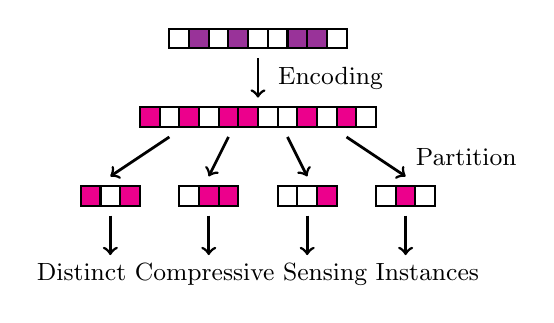
\begin{tikzpicture}
[font=\small, draw=black, line width=0.75pt,
bit0/.style={rectangle, draw, inner sep=0pt, minimum size=2.5mm},
bit1/.style={rectangle, draw, fill=violet!80, inner sep=0pt, minimum size=2.5mm},
ebit0/.style={rectangle, draw, inner sep=0pt, minimum size=2.5mm},
ebit1/.style={rectangle, draw, fill=magenta, inner sep=0pt, minimum size=2.5mm}
]

\node[bit0] (info0) at (0.875,5) {};
\node[bit1] (info1) at (1.125,5) {};
\node[bit0] (info2) at (1.375,5) {};
\node[bit1] (info3) at (1.625,5) {};
\node[bit0] (info4) at (1.875,5) {};
\node[bit0] (info5) at (2.125,5) {};
\node[bit1] (info6) at (2.375,5) {};
\node[bit1] (info7) at (2.625,5) {};
\node[bit0] (info8) at (2.875,5) {};

\draw[->, line width=1pt]  (1.875,4.75) -- (1.875,4.25);
\node[anchor=west] (coding) at (2,4.50) {Encoding};

\node[ebit1] (ebit0) at (0.50,4) {};
\node[ebit0] (ebit1) at (0.75,4) {};
\node[ebit1] (ebit2) at (1.00,4) {};
\node[ebit0] (ebit3) at (1.25,4) {};
\node[ebit1] (ebit4) at (1.50,4) {};
\node[ebit1] (ebit5) at (1.75,4) {};
\node[ebit0] (ebit6) at (2.00,4) {};
\node[ebit0] (ebit7) at (2.25,4) {};
\node[ebit1] (ebit8) at (2.50,4) {};
\node[ebit0] (ebit9) at (2.75,4) {};
\node[ebit1] (ebit10) at (3.00,4) {};
\node[ebit0] (ebit11) at (3.25,4) {};

\draw[->, line width=1pt]  (0.75,3.75) -- (0.00,3.25);
\draw[->, line width=1pt]  (1.50,3.75) -- (1.25,3.25);
\draw[->, line width=1pt]  (2.25,3.75) -- (2.50,3.25);
\draw[->, line width=1pt]  (3.00,3.75) -- (3.75,3.25);
\node[anchor=west] (coding) at (3.75,3.50) {Partition};

\node[ebit1] (s00) at (-0.25,3.00) {};
\node[ebit0] (s01) at (0.00,3.00) {};
\node[ebit1] (s02) at (0.25,3.00) {};

\node[ebit0] (s03) at (1.00,3.00) {};
\node[ebit1] (s04) at (1.25,3.00) {};
\node[ebit1] (s05) at (1.50,3.00) {};

\node[ebit0] (s06) at (2.25,3.00) {};
\node[ebit0] (s07) at (2.50,3.00) {};
\node[ebit1] (s08) at (2.75,3.00) {};

\node[ebit0] (s09) at (3.50,3.00) {};
\node[ebit1] (s10) at (3.75,3.00) {};
\node[ebit0] (s11) at (4.00,3.00) {};

\draw[->, line width=1pt]  (0.00,2.75) -- (0.00,2.25);
\draw[->, line width=1pt]  (1.25,2.75) -- (1.25,2.25);
\draw[->, line width=1pt]  (2.50,2.75) -- (2.50,2.25);
\draw[->, line width=1pt]  (3.75,2.75) -- (3.75,2.25);

\node (cs) at (1.875,2.00) {Distinct Compressive Sensing Instances};
\end{tikzpicture}

\end{center}
\begin{itemize}
\item Split problem into sub-components suitable for CS framework
\item Get lists of sub-packets, one list for every slot
\item Stitch pieces of one packet together using error correction
\end{itemize}
\end{block}
\end{frame}

\begin{frame}
\frametitle{Coded Compressive Sensing -- Device Perspective}
\centerline{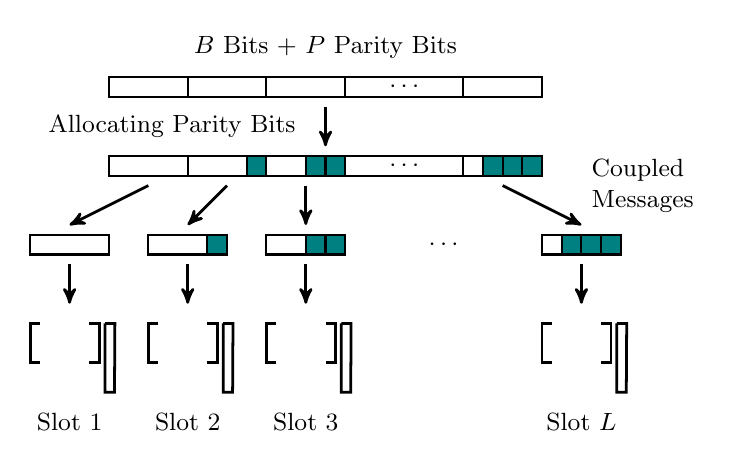
\begin{tikzpicture}
[font=\small, draw=black, line width=0.75pt, >=stealth',
sub0/.style={rectangle, draw, inner sep=0pt, minimum width=10mm,  minimum height=2.5mm},
sub1/.style={rectangle, draw, inner sep=0pt, minimum width=15mm, minimum height=2.5mm},
sub1s/.style={rectangle, inner sep=0pt, minimum width=15mm, minimum height=2.5mm},
parity/.style={rectangle, draw, fill=teal, inner sep=0pt, minimum size=2.5mm}]

\node (coupledvector) at (2.25,5.50) {$B$~Bits + $P$~Parity Bits};
\node[sub0] (cs0) at (0.00,5) {};
\node[sub0] (cs2) at (1.00,5) {};
\node[sub0] (cs3) at (2.00,5) {};
\node[sub1] (csx) at (3.25,5) {$\cdots$};
\node[sub0] (csz) at (4.50,5) {};

\draw[->, line width=1pt]  (2.25,4.75) -- (2.25,4.25);
\node[anchor=east] (coding) at (2.00,4.50) {Allocating Parity Bits};

\node[sub0] (subcs0) at (0.00,4) {};
\node[sub0] (subcs2) at (1.00,4) {};
\node[parity] (parity0) at (1.375,4) {};
\node[sub0] (subcs3) at (2.00,4) {};
\node[parity] (parity1) at (2.125,4) {};
\node[parity] (parity2) at (2.375,4) {};
\node[sub1] (subcsx) at (3.25,4) {$\cdots$};
\node[sub0] (subcsz) at (4.50,4) {};
\node[parity] (parity3) at (4.375,4) {};
\node[parity] (parity4) at (4.625,4) {};
\node[parity] (parity5) at (4.875,4) {};

\node[sub0] (subcs0) at (-1.00,3) {};
\node[sub0] (subcs2) at (0.50,3) {};
\node[parity] (parity0) at (0.875,3) {};
\node[sub0] (subcs3) at (2.00,3) {};
\node[parity] (parity1) at (2.125,3) {};
\node[parity] (parity2) at (2.375,3) {};
\node[sub1s] (subcsx) at (3.75,3) {$\cdots$};
\node[sub0] (subcsz) at (5.50,3) {};
\node[parity] (parity3) at (5.375,3) {};
\node[parity] (parity4) at (5.625,3) {};
\node[parity] (parity5) at (5.875,3) {};

\draw[->, line width=1pt]  (0.00,3.75) -- (-1.00,3.25);
\draw[->, line width=1pt]  (1.00,3.75) -- (0.50,3.25);
\draw[->, line width=1pt]  (2.00,3.75) -- (2.00,3.25);
\draw[->, line width=1pt]  (4.50,3.75) -- (5.50,3.25);
\node[anchor=west,align=left] (coupledvector) at (5.50,3.75) {Coupled\\Messages};

\foreach \v in {-1.00,0.50,2.00,5.50} {
  \draw[->, line width=1pt]  (\v,2.75) -- (\v,2.25);

  \draw[line width=1pt] (\v-0.375,2) -- (\v-0.5,2) -- (\v-0.5,1.5) -- (\v-0.375,1.5);
  \draw[line width=1pt] (\v+0.25,2) -- (\v+0.375,2) -- (\v+0.375,1.5) -- (\v+0.25,1.5);
  \draw[line width=1pt] (\v+0.45,2) -- (\v+0.45,1.125) -- (\v+0.57,1.125) -- (\v+0.575,2) -- (\v+0.45,2);
}

\node (cs) at (-1.00,0.75) {Slot~1};
\node (cs) at (0.50,0.75) {Slot~2};
\node (cs) at (2.00,0.75) {Slot~3};
\node (cs) at (5.50,0.75) {Slot~$L$};
\end{tikzpicture}
}
\vfill
\begin{itemize}
\item Collection of $J$ CS matrices and 1-sparse vectors
\item Each CS generated signal is sent in specific time slot
\end{itemize}
\myfootnote{\tiny
V. Amalladinne, A. Vem, D. Soma, K. R. Narayanan, JFC. \emph{Coupled Compressive Sensing Scheme for Unsourced Multiple Access}. ICASSP 2018}
\end{frame}

\begin{frame}
\frametitle{Coded Compressive Sensing -- Multiple Access}
\centerline{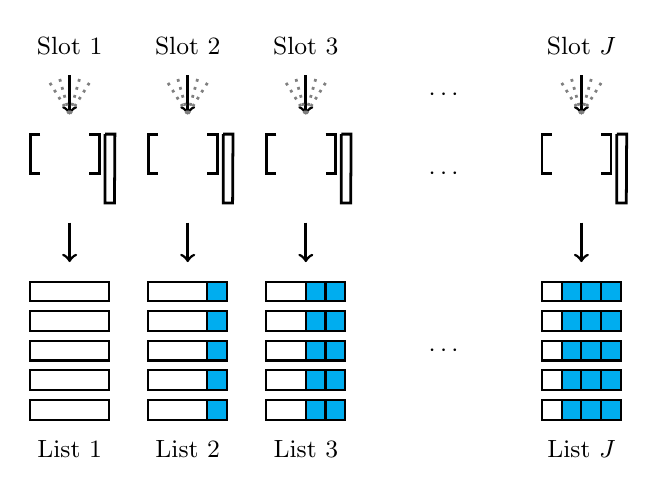
\begin{tikzpicture}
[font=\small, draw=black, line width=0.75pt,
sub0/.style={rectangle, draw, inner sep=0pt, minimum width=10mm, minimum height=2.5mm},
parity/.style={rectangle, draw, fill=cyan, inner sep=0pt, minimum size=2.5mm}]

\node (cs1) at (-1.00,6.125) {Slot~1};
\node (cs2) at (0.50,6.125) {Slot~2};
\node (cs3) at (2.00,6.125) {Slot~3};
\node (cs4) at (5.50,6.125) {Slot~$J$};

\foreach \v in {-1.00,0.50,2.00,5.50} {
  \draw[->, line width=1pt]  (\v,3.875) -- (\v,3.375);
  \draw[->, line width=1pt]  (\v,5.75) -- (\v,5.25);
  \draw[dotted, line width=1pt, draw=gray]  (\v-0.25,5.65) -- (\v,5.25);
  \draw[dotted, line width=1pt, draw=gray]  (\v-0.125,5.7) -- (\v,5.25);
  \draw[dotted, line width=1pt, draw=gray]  (\v+0.125,5.7) -- (\v,5.25);
  \draw[dotted, line width=1pt, draw=gray]  (\v+0.25,5.65) -- (\v,5.25);
}

\node (dots1) at (3.75,5.5) {$\cdots$};

\foreach \v in {-1.00,0.50,2.00,5.50} {
  \draw[line width=1pt] (\v-0.375,5) -- (\v-0.5,5) -- (\v-0.5,4.5) -- (\v-0.375,4.5);
  \draw[line width=1pt] (\v+0.25,5) -- (\v+0.375,5) -- (\v+0.375,4.5) -- (\v+0.25,4.5);
  \draw[line width=1pt] (\v+0.45,5) -- (\v+0.45,4.125) -- (\v+0.57,4.125) -- (\v+0.575,5) -- (\v+0.45,5);
}

\node (dots2) at (3.75,4.5) {$\cdots$};
\node (dots3) at (3.75,2.25) {$\cdots$};

\foreach \c in {3.00, 2.625, 2.25, 1.875, 1.5} {
  \node[sub0] (subcs0\c) at (-1.00,\c) {};
  \node[sub0] (subcs2\c) at (0.50,\c) {};
  \node[parity] (parity0\c) at (0.875,\c) {};
  \node[sub0] (subcs3\c) at (2.00,\c) {};
  \node[parity] (parity1\c) at (2.125,\c) {};
  \node[parity] (parity2\c) at (2.375,\c) {};
  \node[sub0] (subcsz\c) at (5.50,\c) {};
  \node[parity] (parity3\c) at (5.375,\c) {};
  \node[parity] (parity4\c) at (5.625,\c) {};
  \node[parity] (parity5\c) at (5.875,\c) {};
}

\node (list1) at (-1.00,1) {List~1};
\node (list2) at (0.50,1) {List~2};
\node (list3) at (2.00,1) {List~3};
\node (list4) at (5.50,1) {List~$J$};
\end{tikzpicture}
}
\vfill
\begin{itemize}
\item $J$ instances of CS problem, each solved with non-negative LS
\item Produces $J$ lists of $K$ decoded sub-packets (with parity)
\item Must piece sub-packets together using tree decoder
\end{itemize}
\end{frame}


\begin{frame}
\frametitle{Coded Compressive Sensing -- Stitching Process}
  \begin{center}
  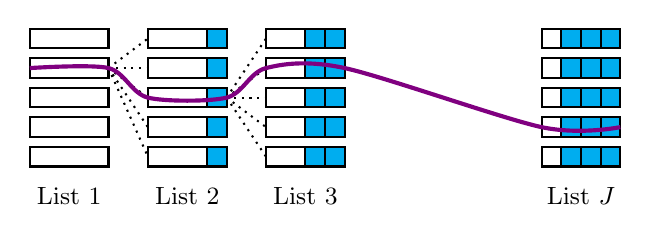
\begin{tikzpicture}
[font=\small, draw=black, line width=0.75pt,
sub0/.style={rectangle, draw, inner sep=0pt, minimum width=10mm, minimum height=2.5mm},
parity/.style={rectangle, draw, fill=cyan, inner sep=0pt, minimum size=2.5mm}]

\foreach \c in {3.00, 2.625, 2.25, 1.875, 1.5} {
  \node[sub0] (subcs1\c) at (-1.00,\c) {};
  \node[sub0] (subcs2\c) at (0.50,\c) {};
  \node[parity] (parity0\c) at (0.875,\c) {};
  \node[sub0] (subcs3\c) at (2.00,\c) {};
  \node[parity] (parity1\c) at (2.125,\c) {};
  \node[parity] (parity2\c) at (2.375,\c) {};
  \node[sub0] (subcsz\c) at (5.50,\c) {};
  \node[parity] (parity3\c) at (5.375,\c) {};
  \node[parity] (parity4\c) at (5.625,\c) {};
  \node[parity] (parity5\c) at (5.875,\c) {};
}

\draw[dotted] (-0.50,2.625) -- (0.00,3.00) {};
\draw[dotted] (-0.50,2.625) -- (0.00,2.625) {};
\draw[dotted] (-0.50,2.625) -- (0.00,2.25) {};
\draw[dotted] (-0.50,2.625) -- (0.00,1.875) {};
\draw[dotted] (-0.50,2.625) -- (0.00,1.50) {};

\draw[dotted] (1.00,2.25) -- (1.50,3.00) {};
\draw[dotted] (1.00,2.25) -- (1.50,2.625) {};
\draw[dotted] (1.00,2.25) -- (1.50,2.25) {};
\draw[dotted] (1.00,2.25) -- (1.50,1.875) {};
\draw[dotted] (1.00,2.25) -- (1.50,1.50) {};

\node (list1) at (-1.00,1) {List~1};
\node (list2) at (0.50,1) {List~2};
\node (list3) at (2.00,1) {List~3};
\node (list4) at (5.50,1) {List~$J$};

\draw [line width=1.5pt,color=violet] plot[smooth, tension=.5] coordinates {
(-1.50,2.625) (-0.50,2.625)
(0.00,2.25) (1.00,2.25)
(1.50,2.625) (2.50,2.625)
(5.00, 1.875) (6.00, 1.875)};
\end{tikzpicture}

  \end{center}
\begin{columns}
\column{.45\textwidth}
\begin{block}{Tree Decoding Principles}
  \begin{itemize}
  \item Every parity is linear combination of bits in preceding blocks
  \item Late parity bits offer better performance
  \item Early parity bits decrease decoding complexity
  \item Correct fragment is on list
  \end{itemize}
\end{block}
\column{.45\textwidth}
  \centerline{\scalebox{0.5}{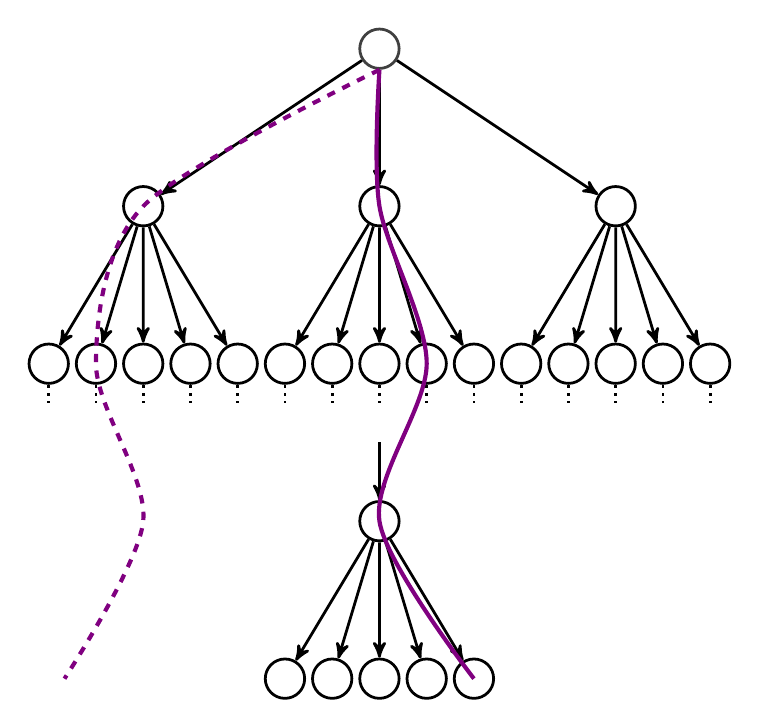
\begin{tikzpicture}
  [
  line width=1pt, draw=black, >=stealth',
  checknode/.style={circle, inner sep=0pt, minimum size=5mm, draw=black}
  ]

  \node[checknode, draw=darkgray] (b1) at (0,4) {};

  \foreach \x in {1,2,3} {
    \node[checknode] (c1\x) at (-6+3*\x,2) {}
      edge[<-] (b1);
  }

  \foreach \y in {1,2,3,4,5} {
    \node[checknode] (b1\y) at (-4.8+0.6*\y,0) {}
      edge[<-] (c11)
      edge[-,dotted] (-4.8+0.6*\y,-0.5);
    \node[checknode] (b2\y) at (-1.8+0.6*\y,0) {}
      edge[<-] (c12)
      edge[-,dotted] (-1.8+0.6*\y,-0.5);
    \node[checknode] (b3\y) at (1.2+0.6*\y,0) {}
      edge[<-] (c13)
      edge[-,dotted] (1.2+0.6*\y,-0.5);
  }
  
  \node[checknode] (c22) at (0,-2) {}
    edge[<-] (0,-1);

  \foreach \y in {1,2,3,4,5} {
    \node[checknode] (b4\y) at (-1.8+0.6*\y,-4) {}
      edge[<-] (c22);
  }

\draw [line width=1.5pt,color=violet] plot[smooth, tension=.5] coordinates {(b1.south) (c12) (b24) (c22) (b45)};
\draw [line width=1.5pt,dashed, color=violet] plot[smooth, tension=.5] coordinates {(b1.south) (c11) (b12) (-3,-2) (-4,-4)};
\end{tikzpicture}
}}
\end{columns}
\end{frame}


\begin{frame}
\frametitle{Coded Compressive Sensing -- Understanding Parity Bits}
\begin{center}
{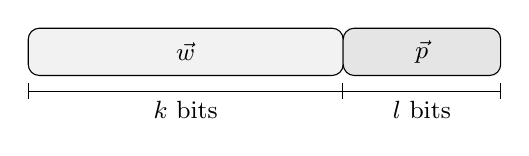
\begin{tikzpicture}[
  font=\small, >=stealth',
  infobits/.style={rectangle, minimum height=6mm, minimum width=40mm, draw=black, fill=gray!10, rounded corners},
  paritybits/.style={rectangle, minimum height=6mm, minimum width=20mm, draw=black, fill=gray!20, rounded corners}
]

\node[infobits] (vb) at (2,0) {$\vec{w}$};
\node[paritybits] (vp) at (5,0) {$\vec{p}$};
\draw[|-|] (0,-0.5) to node[midway,below] {$k$ bits} (4,-0.5);
\draw[-|] (4,-0.5) to node[midway,below] {$l$ bits} (6,-0.5);
\end{tikzpicture}
}
\end{center}
\begin{itemize}
\item Consider binary information vector $\vec{w}$ of length $k$
\item Systematically encoded using generator matrix $G$, with
$\vec{p} = \vec{w} G$
\item Suppose alternate vector $\vec{w}_{\mathrm{r}}$ is selected at random from $\{ 0, 1 \}^k$
\end{itemize}

\begin{block}{Lemma}
Probability that randomly selected information vector $\vec{w}_{\mathrm{r}}$ produces same parity sub-component is given by
\begin{equation*}
\Pr (\vec{p} = \vec{p}_{\mathrm{r}}) = {2^{-\operatorname{rank}(G)}}
\end{equation*}
\end{block}
\textcolor{frametitle.fg}{Proof:}
%\begin{itemize}
%\item Suppose $\vec{w}_{\mathrm{r}}$ is drawn at random from $\{ 0, 1 \}^k$
%\item Then event $\{ \vec{p} = \vec{p}_{\mathrm{r}} \}$ can equivalently be expressed as
%\begin{equation*}
%\begin{split}
$\{ \vec{p} = \vec{p}_{\mathrm{r}} \}
= \{ \vec{w} G = \vec{w}_{\mathrm{r}} G \}
= \{ \vec{w} + \vec{w}_{\mathrm{r}} \in \operatorname{nullspace}(G) \}$
%\end{split}
%\end{equation*}
%\item Number of vectors in nullspace of $G$ is $2^{\operatorname{nullity}(G)} = 2^{k - \operatorname{rank} (G)}$
%\item Then $\Pr ( \vec{p} = \vec{p}_{\mathrm{r}} )
%= \frac{2^{k - \operatorname{rank} (G)}}{2^k}
%= 2^{- \operatorname{rank} (G)}$
%\end{itemize}
\end{frame}

\begin{frame}
\frametitle{Coded Compressive Sensing -- General Parity Bits}
\begin{center}
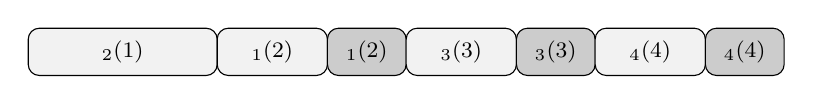
\begin{tikzpicture}[
  font=\footnotesize, >=stealth',
  infobits0/.style={rectangle, minimum height=6mm, minimum width=24mm, draw=black, fill=gray!10, rounded corners},
  infobits/.style={rectangle, minimum height=6mm, minimum width=14mm, draw=black, fill=gray!10, rounded corners},
  paritybits/.style={rectangle, minimum height=6mm, minimum width=10mm, draw=black, fill=gray!40, rounded corners}
]

\node[infobits0] (vb0) at (1.2,0) {$\wv_2(1)$};
\node[infobits] (vb1) at (3.1,0) {$\wv_1(2)$};
\node[paritybits] (vp1) at (4.3,0) {$\pv_1(2)$};
\node[infobits] (vb2) at (5.5,0) {$\wv_3(3)$};
\node[paritybits] (vp2) at (6.7,0) {$\pv_3(3)$};
\node[infobits] (vb3) at (7.9,0) {$\wv_4(4)$};
\node[paritybits] (vp3) at (9.1,0) {$\pv_4(4)$};
\end{tikzpicture}

\end{center}
\begin{itemize}
\item True vector $(\vec{w}_{i_0}(0), \vec{w}_{i_0}(1), \vec{w}_{i_0}(2), \vec{w}_{i_0}(3))$
\item Consider alternate vector with information sub-block $(\vec{w}_{i_0}(0), \vec{w}_{i_1}(1), \vec{w}_{i_2}(2), \vec{w}_{i_3}(3))$ pieced from lists
\item To survive stage~3, candidate vector must fulfill parity equations
\end{itemize}
\begin{align*}
\left( \vec{w}_{i_0}(0) - \vec{w}_{i_1}(0) \right) \begin{bmatrix} G_{0,0} \end{bmatrix} &= \vec{0}_{1 \times l_1} \\
\left( \vec{w}_{i_0}(0) - \vec{w}_{i_2}(0), \vec{w}_{i_1}(1) - \vec{w}_{i_2}(1) \right)
\begin{bmatrix} G_{0,1} \\ G_{1,1} \end{bmatrix}
&= \vec{0}_{1 \times l_2} \\
\left( \vec{w}_{i_0}(0) - \vec{w}_{i_3}(0), \vec{w}_{i_1}(1) - \vec{w}_{i_3}(1), \vec{w}_{i_2}(2) - \vec{w}_{i_3}(2) \right)
\begin{bmatrix} G_{0,2} \\ G_{1,2} \\ G_{2,2} \end{bmatrix}
&= \vec{0}_{1 \times l_3}
\end{align*}
\end{frame}

\begin{frame}
\frametitle{Coded Compressive Sensing -- General Parity Bits}
\begin{center}
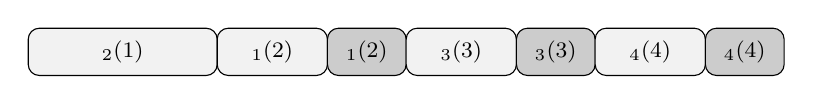
\begin{tikzpicture}[
  font=\footnotesize, >=stealth',
  infobits0/.style={rectangle, minimum height=6mm, minimum width=24mm, draw=black, fill=gray!10, rounded corners},
  infobits/.style={rectangle, minimum height=6mm, minimum width=14mm, draw=black, fill=gray!10, rounded corners},
  paritybits/.style={rectangle, minimum height=6mm, minimum width=10mm, draw=black, fill=gray!40, rounded corners}
]

\node[infobits0] (vb0) at (1.2,0) {$\wv_2(1)$};
\node[infobits] (vb1) at (3.1,0) {$\wv_1(2)$};
\node[paritybits] (vp1) at (4.3,0) {$\pv_1(2)$};
\node[infobits] (vb2) at (5.5,0) {$\wv_3(3)$};
\node[paritybits] (vp2) at (6.7,0) {$\pv_3(3)$};
\node[infobits] (vb3) at (7.9,0) {$\wv_4(4)$};
\node[paritybits] (vp3) at (9.1,0) {$\pv_4(4)$};
\end{tikzpicture}

\end{center}
\begin{itemize}
\item When indices are not repeated in $(\vec{w}_{i_0}(0), \vec{w}_{i_1}(1), \vec{w}_{i_2}(2), \vec{w}_{i_3}(3))$, probability is governed by
\begin{equation*}
\operatorname{rank}
\left(
\begin{bmatrix}
G_{0,0} & G_{0,1} & G_{0,2} \\
\mathbf{0} & G_{1,1} & G_{1,2} \\
\mathbf{0} & \mathbf{0}& G_{2,2}
\end{bmatrix}
\right)
\end{equation*}
\item \textcolor{gray}{But, when indices are repeated, sub-blocks may disappear
\begin{equation*}
\operatorname{rank}
\left(
\begin{bmatrix}
G_{0,0} \mathbf{1}_{\{ i_1 \neq i_0 \}} & G_{0,1} \mathbf{1}_{\{ i_2 \neq i_0 \}} & G_{0,2} \mathbf{1}_{\{ i_3 \neq i_0 \}} \\
\mathbf{0} & G_{1,1} \mathbf{1}_{\{ i_2 \neq i_1 \}} & G_{1,2} \mathbf{1}_{\{ i_3 \neq i_1 \}} \\
\mathbf{0} & \mathbf{0}& G_{2,2} \mathbf{1}_{\{ i_3 \neq i_2 \}}
\end{bmatrix}
\right)
\end{equation*}}
\end{itemize}
\end{frame}


\begin{frame}
\frametitle{Allocating Parity Bits (approximation)}
\begin{itemize}
\item $l_i$: \# parity bits in sub-block $i \in 2, \ldots, J$,
\item $L_i$: \# erroneous paths that survive stage $i \in 2, \ldots, J$,
\item Complexity $C_{\mathrm{tree}}$: \# nodes on which parity check constraints verified
\end{itemize}
\begin{block}{Expressions for $\mathbb{E}[L_i]$ and $C_{\mathrm{tree}}$}
\begin{itemize}
\item $L_i \lvert L_{i-1} \sim B((L_{i-1}+1)K-1,p_i)$, $p_i=2^{-l_i}$, $q_i=1-p_i$
\begin{align*}
\mathbb{E}[L_i] &= \mathbb{E}[ \mathbb{E}[L_i \lvert L_{i-1}]] \\
&= \mathbb{E}[((L_{i-1}+1)K-1)p_i] \\
&= p_iK\mathbb{E}[L_{i-1}] + p_i(K-1) \\
&= \sum_{r=1}^{i} K^{i-r}(K-1) \prod_{j=r}^{i}p_j
\end{align*}
\item $C_{\mathrm{tree}} = K + \sum_{i=1}^{J-2}\left[(L_i + 1)K\right]$
\item $\mathbb{E}[C_{\mathrm{tree}}]$ can be computed using the expression for $\mathbb{E}[L_i]$
\end{itemize}
\end{block}
\end{frame}


\begin{frame}
\frametitle{Optimization of Parity Lengths}
\begin{itemize}
\item $l_i$: \# parity bits in sub-block $i \in 2, \ldots, J$,
\item $L_i$: \# erroneous paths that survive stage $i \in 2, \ldots, J$,
\end{itemize}
\begin{block}{(Relaxed) Geometric Programming Optimization}
\begin{equation*}
\begin{aligned}
& \underset{(l_2, \dots, l_{J})}{\text{minimize}}
& &\mathbb{E}[C_{\mathrm{tree}}] \\
& \text{subject to}
& & \Pr(L_{J} \ge 1) \le \varepsilon_{\mathrm{tree}}
& \text{\textcolor{frametitle.fg}{Erroneous Paths}} \\
&&& \sum_{i=2}^{J} l_i = M-B & \text{\textcolor{frametitle.fg}{Total \# Parity Bits}} \\
&&& l_i \in \{ 0, \ldots, N/J \} \quad \forall~i \in 2, \ldots, J
& \text{\textcolor{frametitle.fg}{Integer Constraints}}
\end{aligned}
\end{equation*}
\begin{itemize}
\item Can be solved using standard convex solver (e.g.~CVX)
\end{itemize}
\end{block}
\end{frame}


\begin{frame}
\frametitle{Choice of Parity Lengths}
\begin{itemize}
\item $K=200$, $J=11$, $N/J=15$
\end{itemize}
\begin{center}
\begin{tabular}{||l|l|l||}
\hline
 $\varepsilon_{\mathrm{tree}}$ & $\mathbb{E}[C_{\mathrm{tree}}]$ & Parity Lengths $l_2, \ldots, l_J$ \\ [0.5ex]
\hline \hline
$0.006$ & Infeasible & Infeasible \\
\hline
$0.0061930$ & $3.2357\times10^{11}$ & $ 0 ,0, 0, 0, 15, 15, 15, 15, 15, 15$ \\
\hline
$0.0061931$ & $3357300$ & $ 0, 3, 8, 8, 8, 8, 10, 15, 15, 15$ \\
\hline
$0.0061932$ & $1737000$ & $ 0, 4, 8, 8, 8, 8, 9, 15, 15, 15$ \\
\hline
$0.0061933$ & $926990$ & $ 0, 5, 8, 8, 8, 8, 8, 15, 15, 15$ \\
\hline
$0.0061935$ & $467060$ & $ 1, 8, 8, 8, 8, 8, 8, 11, 15, 15$ \\
\hline
$0.0062$ & $79634$ & $ 1, 8, 8, 8, 8, 8, 8, 11, 15, 15$ \\
\hline
$0.007$ & $7357.8$ & $ 6, 8, 8, 8, 8, 8, 8, 8, 13, 15$ \\
\hline
$0.008$ & $6152.7$ & $ 7, 8, 8, 8, 8, 8, 8, 8, 12, 15$ \\
\hline
$0.02$ & $5022.9$ & $ 6, 8, 8, 9, 9, 9, 9, 9, 9, 14$ \\
\hline
$0.04$ & $4158$ & $ 7, 8, 8, 9, 9, 9, 9, 9, 9, 13$ \\
\hline
$0.6378$ & $3066.3$ & $ 9, 9, 9, 9, 9, 9, 9, 9, 9, 9$ \\ [1ex]
\hline
\end{tabular}
\end{center}
\end{frame}


\begin{frame}
\frametitle{Leveraging CCS Framework}
\begin{center}
\begin{tikzpicture}
  \node[scope fading=south] (image) at (0,0) {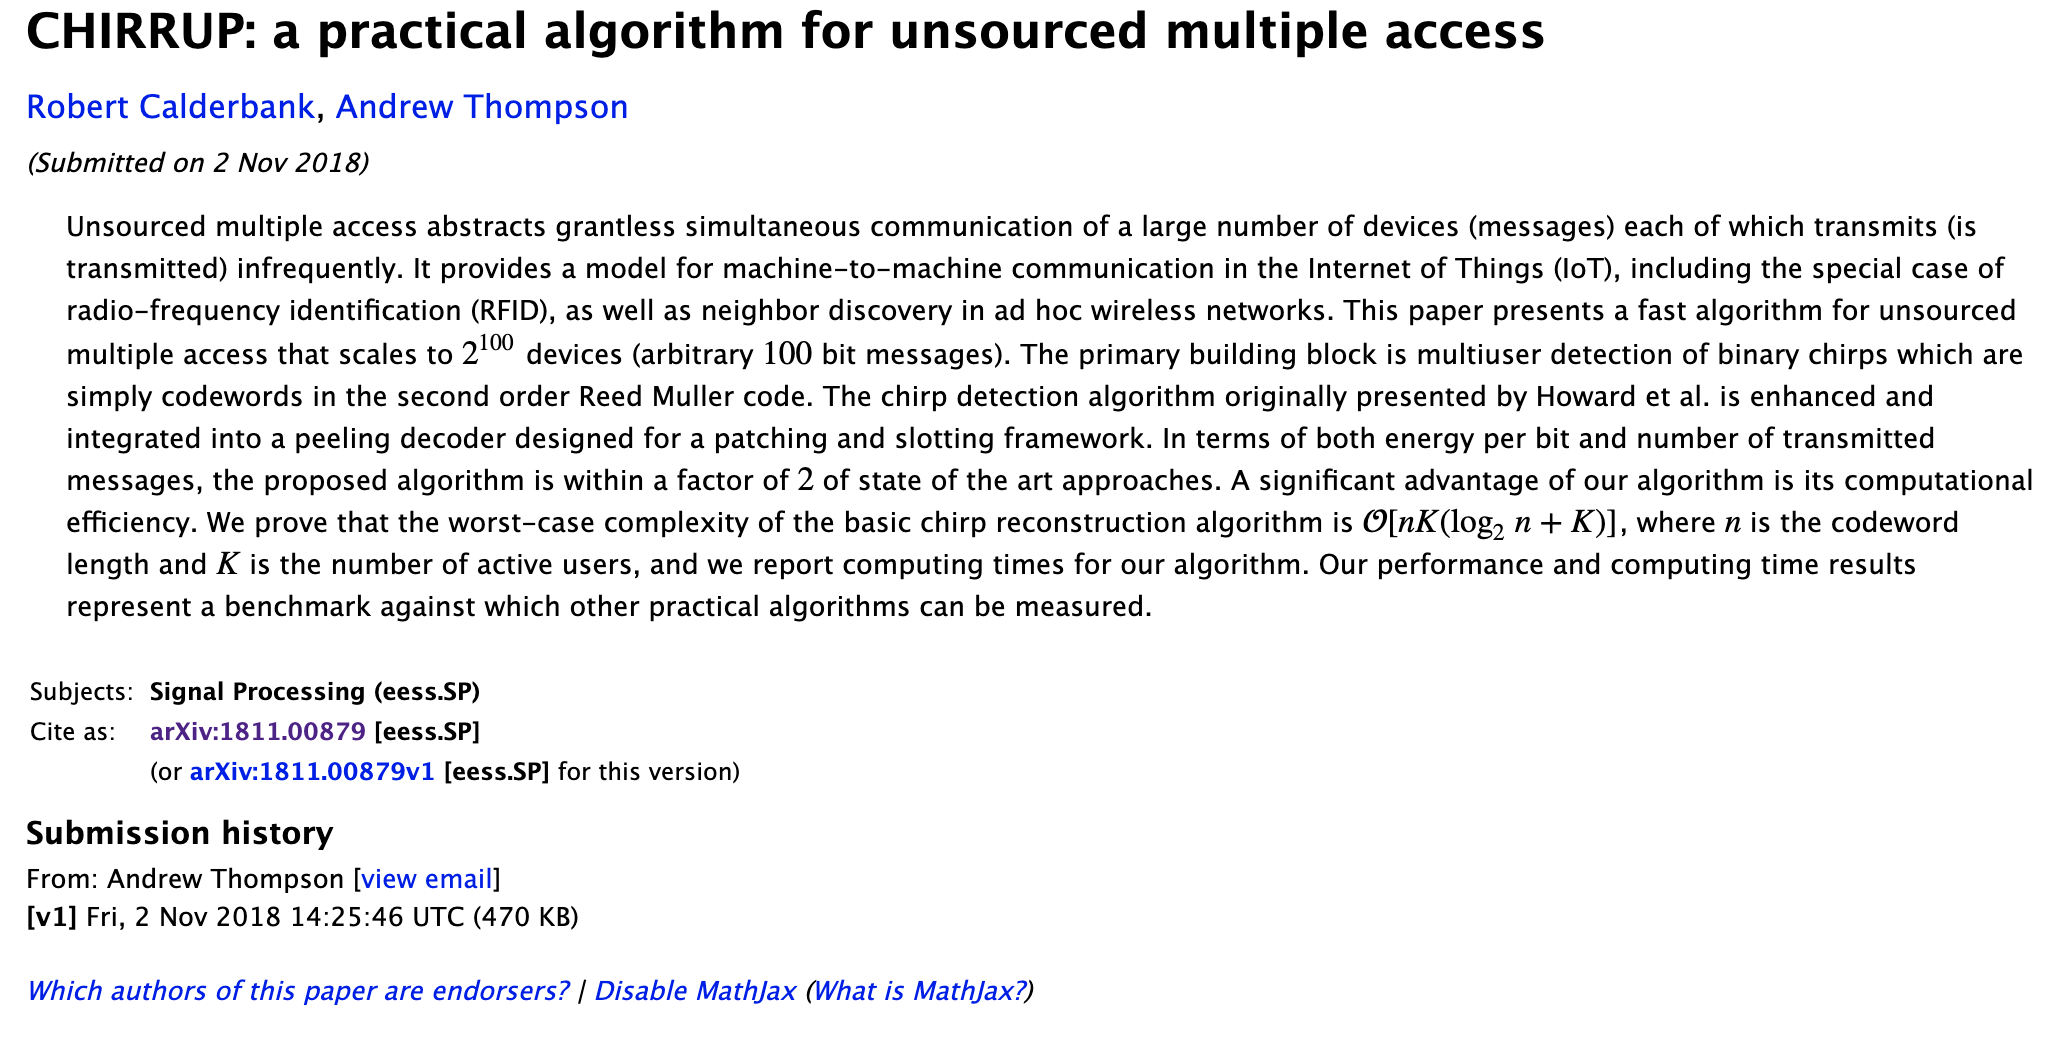
\includegraphics[width=4in]{Figures/CHIRRUP.png}};
\end{tikzpicture}
\end{center}
  \begin{itemize}
  \item Robert Calderbank, Andrew Thompson on arXiv
  \item Hadamard matrix based compressing scheme $+$  CSS
  \item Ultra-low complexity decoding algorithm
  \end{itemize}
\end{frame}


\part{Quest for Low-Complexity: \newline Hybrid and Emerging Paradigms}
\frame{\partpage}
\begin{frame}
\frametitle{Extending CCS Framework}
\begin{center}
\begin{tikzpicture}
  \node[scope fading=south] (image) at (0,0) {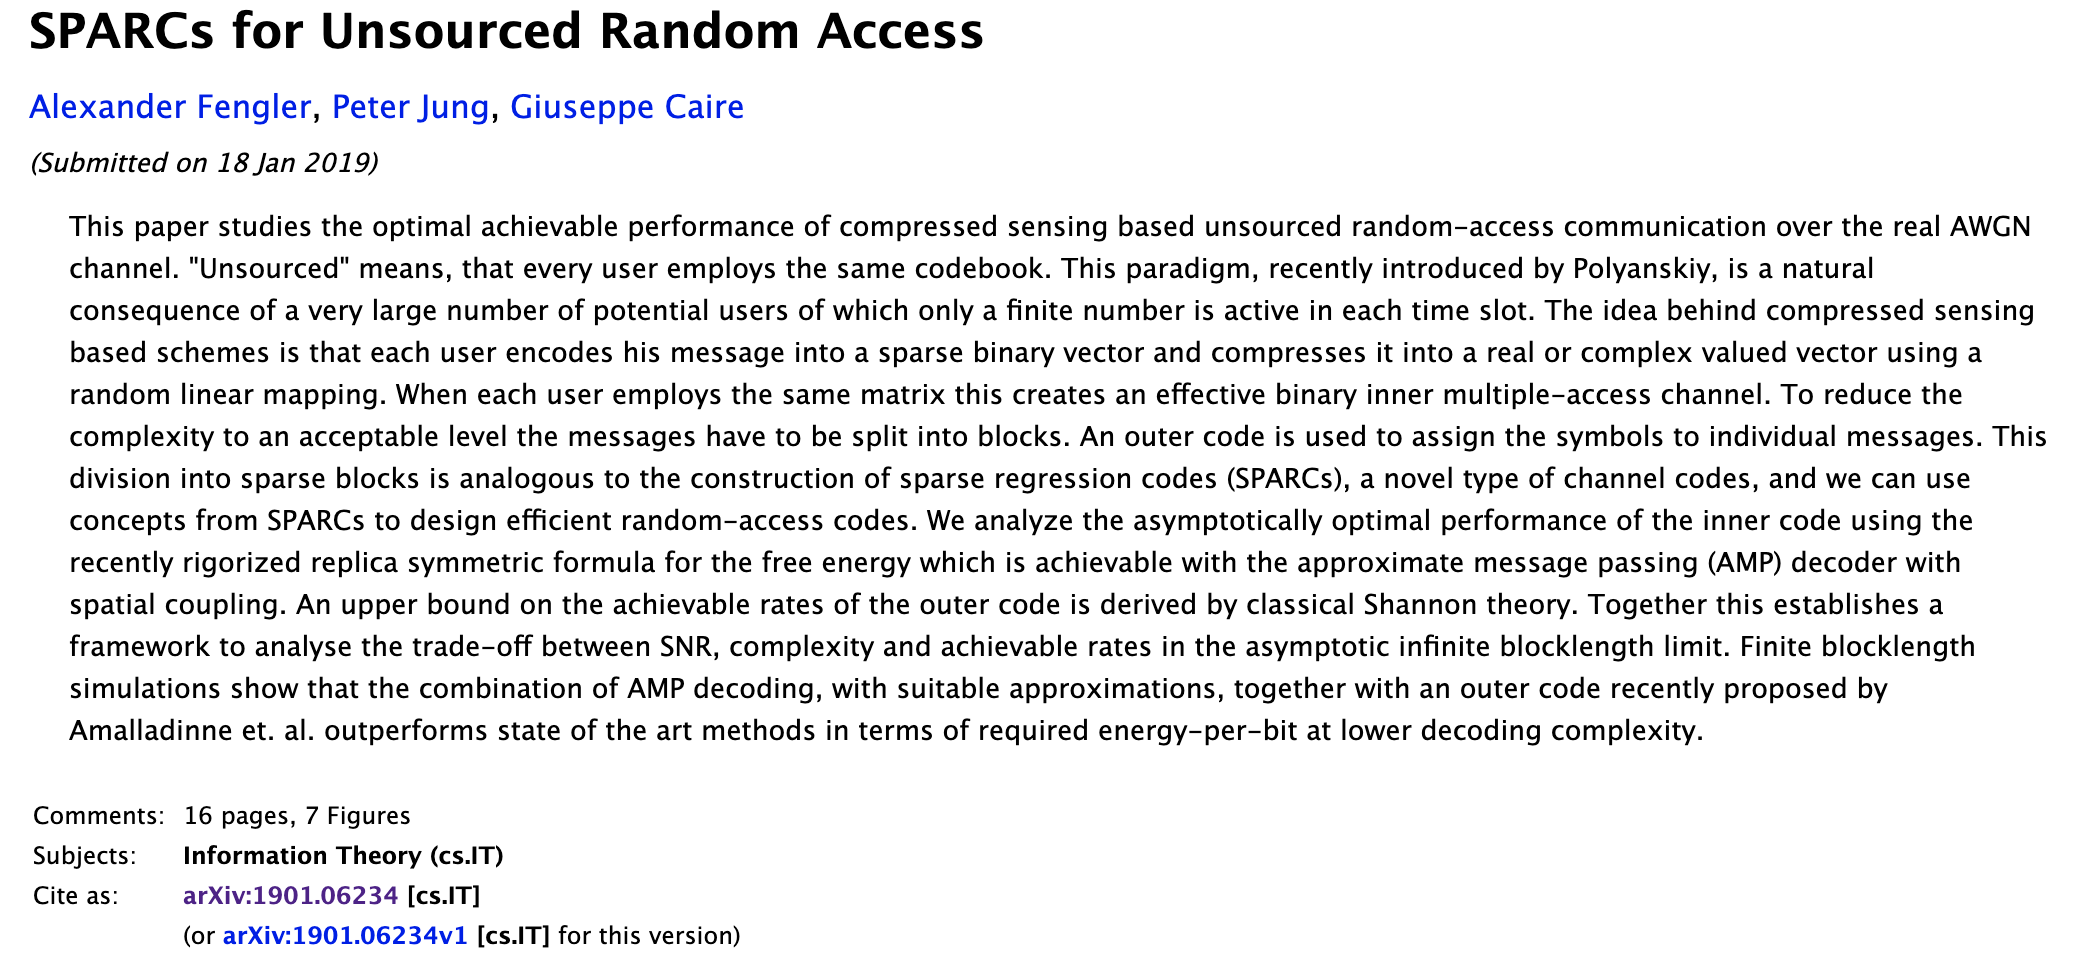
\includegraphics[width=4in]{Figures/SparcsUMAC.png}};
\end{tikzpicture}
\end{center}
  \begin{itemize}
  \item Alexander Fengler, Peter Jung, Giuseppe Caire on arXiv
  \item Connection between CCS indexing and sparse regression codes
  \item Circumvent slotting under CCS and dispersion effects
  \end{itemize}
\end{frame}


\begin{frame}
\frametitle{UMAC -- CCS Revisited}
\begin{center}
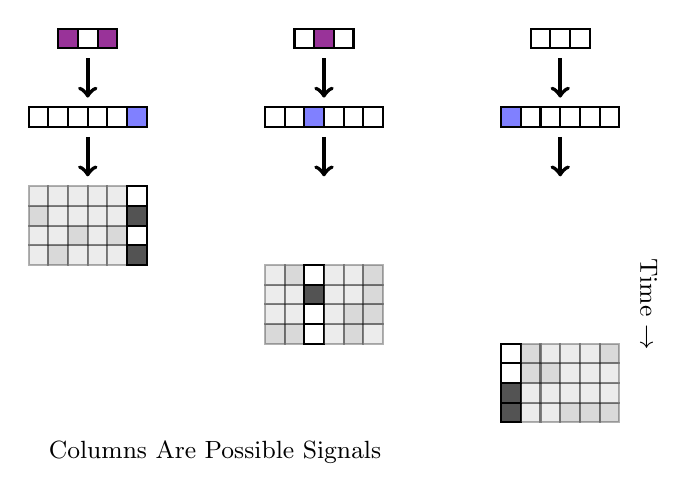
\begin{tikzpicture}
[font=\small, draw=black, line width=0.75pt,
bit0/.style={rectangle, draw, inner sep=0pt, minimum size=2.5mm},
bit1/.style={rectangle, draw, fill=violet!80, inner sep=0pt, minimum size=2.5mm},
entry0/.style={rectangle, draw, opacity=0.3, fill=lightgray, inner sep=0pt, minimum size=2.5mm},
entry1/.style={rectangle, draw, opacity=0.3, fill=gray, inner sep=0pt, minimum size=2.5mm},
entry00/.style={rectangle, draw, fill=white, inner sep=0pt, minimum size=2.5mm},
entry11/.style={rectangle, draw, fill=darkgray!90, inner sep=0pt, minimum size=2.5mm},
symbol0/.style={rectangle, draw, fill=white, inner sep=0pt, minimum size=2.5mm},
symbol1/.style={rectangle, draw, fill=blue!50, inner sep=0pt, minimum size=2.5mm}]

\node[entry11] (m2400) at (6.00,0) {};
\node[entry0] (m2500) at (6.25,0) {};
\node[entry0] (m2600) at (6.50,0) {};
\node[entry1] (m2700) at (6.75,0) {};
\node[entry1] (m2800) at (7.00,0) {};
\node[entry1] (m2900) at (7.25,0) {};

\node[entry11] (m2401) at (6.00,0.25) {};
\node[entry0] (m2501) at (6.25,0.25) {};
\node[entry0] (m2601) at (6.50,0.25) {};
\node[entry0] (m2701) at (6.75,0.25) {};
\node[entry0] (m2801) at (7.00,0.25) {};
\node[entry0] (m2901) at (7.25,0.25) {};

\node[entry00] (m2402) at (6.00,0.50) {};
\node[entry1] (m2502) at (6.25,0.50) {};
\node[entry1] (m2602) at (6.50,0.50) {};
\node[entry0] (m2702) at (6.75,0.50) {};
\node[entry0] (m2802) at (7.00,0.50) {};
\node[entry0] (m2902) at (7.25,0.50) {};

\node[entry00] (m2403) at (6.00,0.75) {};
\node[entry1] (m2503) at (6.25,0.75) {};
\node[entry0] (m2603) at (6.50,0.75) {};
\node[entry0] (m2703) at (6.75,0.75) {};
\node[entry0] (m2803) at (7.00,0.75) {};
\node[entry1] (m2903) at (7.25,0.75) {};

\node[entry1] (m1204) at (3.00,1.00) {};
\node[entry1] (m1304) at (3.25,1.00) {};
\node[entry00] (m1404) at (3.50,1.00) {};
\node[entry0] (m1504) at (3.75,1.00) {};
\node[entry1] (m1604) at (4.00,1.00) {};
\node[entry0] (m1704) at (4.25,1.00) {};

\node[entry0] (m1205) at (3.00,1.25) {};
\node[entry0] (m1305) at (3.25,1.25) {};
\node[entry00] (m1405) at (3.50,1.25) {};
\node[entry0] (m1505) at (3.75,1.25) {};
\node[entry1] (m1605) at (4.00,1.25) {};
\node[entry1] (m1705) at (4.25,1.25) {};

\node[entry0] (m1206) at (3.00,1.50) {};
\node[entry0] (m1306) at (3.25,1.50) {};
\node[entry11] (m1406) at (3.50,1.50) {};
\node[entry0] (m1506) at (3.75,1.50) {};
\node[entry0] (m1606) at (4.00,1.50) {};
\node[entry1] (m1706) at (4.25,1.50) {};

\node[entry0] (m1207) at (3.00,1.75) {};
\node[entry1] (m1307) at (3.25,1.75) {};
\node[entry00] (m1407) at (3.50,1.75) {};
\node[entry0] (m1507) at (3.75,1.75) {};
\node[entry0] (m1607) at (4.00,1.75) {};
\node[entry1] (m1707) at (4.25,1.75) {};

\node[entry0] (m0008) at (0.00,2.00) {};
\node[entry1] (m0108) at (0.25,2.00) {};
\node[entry0] (m0208) at (0.50,2.00) {};
\node[entry0] (m0308) at (0.75,2.00) {};
\node[entry0] (m0408) at (1.00,2.00) {};
\node[entry11] (m0508) at (1.25,2.00) {};

\node[entry0] (m0009) at (0.00,2.25) {};
\node[entry0] (m0109) at (0.25,2.25) {};
\node[entry1] (m0209) at (0.50,2.25) {};
\node[entry0] (m0309) at (0.75,2.25) {};
\node[entry1] (m0409) at (1.00,2.25) {};
\node[entry00] (m0509) at (1.25,2.25) {};

\node[entry1] (m0010) at (0.00,2.50) {};
\node[entry0] (m0110) at (0.25,2.50) {};
\node[entry0] (m0210) at (0.50,2.50) {};
\node[entry0] (m0310) at (0.75,2.50) {};
\node[entry0] (m0410) at (1.00,2.50) {};
\node[entry11] (m0510) at (1.25,2.50) {};

\node[entry0] (m0011) at (0.00,2.75) {};
\node[entry0] (m0111) at (0.25,2.75) {};
\node[entry0] (m0211) at (0.50,2.75) {};
\node[entry0] (m0311) at (0.75,2.75) {};
\node[entry0] (m0411) at (1.00,2.75) {};
\node[entry00] (m0511) at (1.25,2.75) {};

\draw[->, line width=1.5pt]  (0.625,3.50) -- (0.625,3.00);
\draw[->, line width=1.5pt]  (3.625,3.50) -- (3.625,3.00);
\draw[->, line width=1.5pt]  (6.625,3.50) -- (6.625,3.00);

\node[symbol0] (s00) at (0.00,3.75) {};
\node[symbol0] (s01) at (0.25,3.75) {};
\node[symbol0] (s02) at (0.50,3.75) {};
\node[symbol0] (s03) at (0.75,3.75) {};
\node[symbol0] (s04) at (1.00,3.75) {};
\node[symbol1] (s05) at (1.25,3.75) {};

\node[symbol0] (s12) at (3.00,3.75) {};
\node[symbol0] (s13) at (3.25,3.75) {};
\node[symbol1] (s14) at (3.50,3.75) {};
\node[symbol0] (s15) at (3.75,3.75) {};
\node[symbol0] (s16) at (4.00,3.75) {};
\node[symbol0] (s17) at (4.25,3.75) {};

\node[symbol1] (s24) at (6.00,3.75) {};
\node[symbol0] (s25) at (6.25,3.75) {};
\node[symbol0] (s26) at (6.50,3.75) {};
\node[symbol0] (s27) at (6.75,3.75) {};
\node[symbol0] (s28) at (7.00,3.75) {};
\node[symbol0] (s29) at (7.25,3.75) {};

\draw[->, line width=1.5pt]  (0.625,4.50) -- (0.625,4.00);
\draw[->, line width=1.5pt]  (3.625,4.50) -- (3.625,4.00);
\draw[->, line width=1.5pt]  (6.625,4.50) -- (6.625,4.00);

\node[bit1] (info0) at (0.375,4.75) {};
\node[bit0] (info1) at (0.625,4.75) {};
\node[bit1] (info2) at (0.875,4.75) {};
\node[bit0] (info3) at (3.375,4.75) {};
\node[bit1] (info4) at (3.625,4.75) {};
\node[bit0] (info5) at (3.875,4.75) {};
\node[bit0] (info6) at (6.375,4.75) {};
\node[bit0] (info7) at (6.625,4.75) {};
\node[bit0] (info8) at (6.875,4.75) {};


\node [anchor = west] (signals) at (0.00,-0.50) {Columns Are Possible Signals};
\node[rotate=-90] (time) at (7.75,1.375) {Time $\rightarrow$};
\end{tikzpicture}

\end{center}
\begin{itemize}
\item Bit sequence split into $J$ fragments
\item Each bit $+$ parity block converted to index in $[ 1, 2^{M/J} ]$
\item Stack sub-codewords into $(N/J) \times 2^{M/J}$ sensing matrices
\end{itemize}
\end{frame}

\begin{frame}
\frametitle{UMAC -- CCS Unified CS Analogy}
\centerline{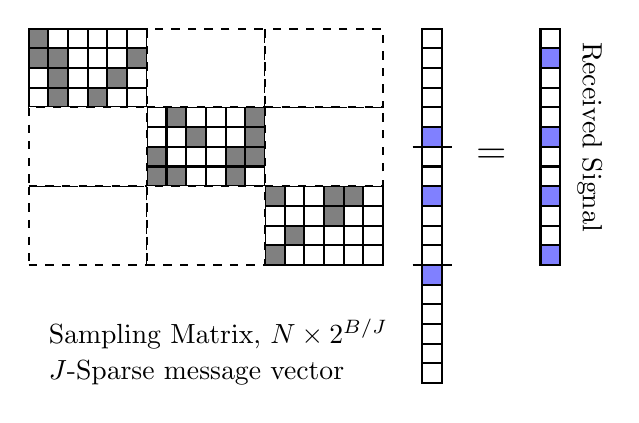
\begin{tikzpicture}
[draw=black, line width=0.75pt,
block/.style={rectangle, draw, fill=white, inner sep=0pt, minimum width=15mm,minimum height=10mm},
entry1/.style={rectangle, draw, fill=gray, inner sep=0pt, minimum size=2.5mm},
entry0/.style={rectangle, draw, fill=white, inner sep=0pt, minimum size=2.5mm},
symbol0/.style={rectangle, draw, fill=white, inner sep=0pt, minimum size=2.5mm},
symbol1/.style={rectangle, draw, fill=blue!50, inner sep=0pt, minimum size=2.5mm}]

\node[entry1] (m1800) at (4.50,0) {};
\node[entry0] (m1900) at (4.75,0) {};
\node[entry0] (m2000) at (5.00,0) {};
\node[entry0] (m2100) at (5.25,0) {};
\node[entry0] (m2200) at (5.50,0) {};
\node[entry0] (m2300) at (5.75,0) {};

\node[entry0] (m1801) at (4.50,0.25) {};
\node[entry1] (m1901) at (4.75,0.25) {};
\node[entry0] (m2001) at (5.00,0.25) {};
\node[entry0] (m2101) at (5.25,0.25) {};
\node[entry0] (m2201) at (5.50,0.25) {};
\node[entry0] (m2301) at (5.75,0.25) {};

\node[entry0] (m1802) at (4.50,0.50) {};
\node[entry0] (m1902) at (4.75,0.50) {};
\node[entry0] (m2002) at (5.00,0.50) {};
\node[entry1] (m2102) at (5.25,0.50) {};
\node[entry0] (m2202) at (5.50,0.50) {};
\node[entry0] (m2302) at (5.75,0.50) {};

\node[entry1] (m1803) at (4.50,0.75) {};
\node[entry0] (m1903) at (4.75,0.75) {};
\node[entry0] (m2003) at (5.00,0.75) {};
\node[entry1] (m2103) at (5.25,0.75) {};
\node[entry1] (m2203) at (5.50,0.75) {};
\node[entry0] (m2303) at (5.75,0.75) {};

\node[entry1] (m1204) at (3.00,1.00) {};
\node[entry1] (m1304) at (3.25,1.00) {};
\node[entry0] (m1404) at (3.50,1.00) {};
\node[entry0] (m1504) at (3.75,1.00) {};
\node[entry1] (m1604) at (4.00,1.00) {};
\node[entry0] (m1704) at (4.25,1.00) {};

\node[entry1] (m1205) at (3.00,1.25) {};
\node[entry0] (m1305) at (3.25,1.25) {};
\node[entry0] (m1405) at (3.50,1.25) {};
\node[entry0] (m1505) at (3.75,1.25) {};
\node[entry1] (m1605) at (4.00,1.25) {};
\node[entry1] (m1705) at (4.25,1.25) {};

\node[entry0] (m1206) at (3.00,1.50) {};
\node[entry0] (m1306) at (3.25,1.50) {};
\node[entry1] (m1406) at (3.50,1.50) {};
\node[entry0] (m1506) at (3.75,1.50) {};
\node[entry0] (m1606) at (4.00,1.50) {};
\node[entry1] (m1706) at (4.25,1.50) {};

\node[entry0] (m1207) at (3.00,1.75) {};
\node[entry1] (m1307) at (3.25,1.75) {};
\node[entry0] (m1407) at (3.50,1.75) {};
\node[entry0] (m1507) at (3.75,1.75) {};
\node[entry0] (m1607) at (4.00,1.75) {};
\node[entry1] (m1707) at (4.25,1.75) {};

\node[entry0] (m0608) at (1.50,2.00) {};
\node[entry1] (m0708) at (1.75,2.00) {};
\node[entry0] (m0808) at (2.00,2.00) {};
\node[entry1] (m0908) at (2.25,2.00) {};
\node[entry0] (m1008) at (2.50,2.00) {};
\node[entry0] (m1108) at (2.75,2.00) {};

\node[entry0] (m0609) at (1.50,2.25) {};
\node[entry1] (m0709) at (1.75,2.25) {};
\node[entry0] (m0809) at (2.00,2.25) {};
\node[entry0] (m0909) at (2.25,2.25) {};
\node[entry1] (m1009) at (2.50,2.25) {};
\node[entry0] (m1109) at (2.75,2.25) {};

\node[entry1] (m0610) at (1.50,2.50) {};
\node[entry1] (m0710) at (1.75,2.50) {};
\node[entry0] (m0810) at (2.00,2.50) {};
\node[entry0] (m0910) at (2.25,2.50) {};
\node[entry0] (m1010) at (2.50,2.50) {};
\node[entry1] (m1110) at (2.75,2.50) {};

\node[entry1] (m0611) at (1.50,2.75) {};
\node[entry0] (m0711) at (1.75,2.75) {};
\node[entry0] (m0811) at (2.00,2.75) {};
\node[entry0] (m0911) at (2.25,2.75) {};
\node[entry0] (m1011) at (2.50,2.75) {};
\node[entry0] (m1111) at (2.75,2.75) {};

\node[block,dashed] at (2.125,0.375) {};
\node[block,dashed] at (2.125,1.375) {};
\node[block,dashed] at (3.625,0.375) {};
\node[block,dashed] at (3.625,2.375) {};
\node[block,dashed] at (5.125,1.375) {};
\node[block,dashed] at (5.125,2.375) {};

\node[symbol0] (s07) at (6.5,-1.50) {};
\node[symbol0] (s08) at (6.5,-1.25) {};
\node[symbol0] (s09) at (6.5,-1.00) {};
\node[symbol0] (s10) at (6.5,-0.75) {};
\node[symbol0] (s11) at (6.5,-0.50) {};
\node[symbol1] (s12) at (6.5,-0.25) {};
\draw (6.25,-0.125) -- (6.75,-0.125);
\node[symbol0] (s13) at (6.5,0) {};
\node[symbol0] (s14) at (6.5,0.25) {};
\node[symbol0] (s15) at (6.5,0.50) {};
\node[symbol1] (s16) at (6.5,0.75) {};
\node[symbol0] (s17) at (6.5,1.00) {};
\node[symbol0] (s18) at (6.5,1.25) {};
\draw (6.25,1.375) -- (6.75,1.375);
\node[symbol1] (s19) at (6.5,1.50) {};
\node[symbol0] (s20) at (6.5,1.75) {};
\node[symbol0] (s21) at (6.5,2.00) {};
\node[symbol0] (s22) at (6.5,2.25) {};
\node[symbol0] (s23) at (6.5,2.50) {};
\node[symbol0] (s24) at (6.5,2.75) {};

\node (equal) at (7.25,1.25) {\Large =};

\node[symbol1] (y00) at (8,0) {};
\node[symbol0] (y01) at (8,0.25) {};
\node[symbol0] (y02) at (8,0.50) {};
\node[symbol1] (y03) at (8,0.75) {};
\node[symbol0] (y04) at (8,1.00) {};
\node[symbol0] (y05) at (8,1.25) {};
\node[symbol1] (y06) at (8,1.50) {};
\node[symbol0] (y07) at (8,1.75) {};
\node[symbol0] (y08) at (8,2.00) {};
\node[symbol0] (y09) at (8,2.25) {};
\node[symbol1] (y10) at (8,2.50) {};
\node[symbol0] (y11) at (8,2.75) {};

\node[anchor=west] (samplingmatrix) at (1.5,-1) {Sampling Matrix, $N \times 2^{{B}/{J}}$};
\node[anchor=west] (vector) at (1.5,-1.5) {$J$-Sparse message vector};
\node[rotate=-90] (receivedsignal) at (8.5,1.5) {Received Signal};
\end{tikzpicture}
}
\begin{itemize}
\item Initial non-linear indexing step
\item Index vector is $J$-block sparse
\item Connection to sparse regression codes
\end{itemize}
\end{frame}


\begin{frame}
\frametitle{UMAC -- Exact CS Analogy}
\centerline{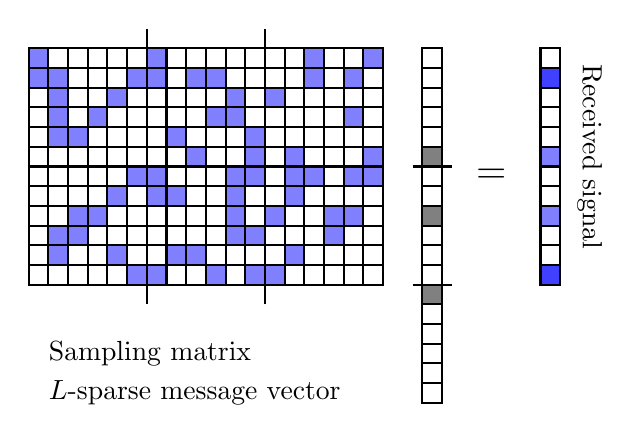
\begin{tikzpicture}
[draw=black, line width=0.75pt,
entry0/.style={rectangle, draw, fill=white, inner sep=0pt, minimum size=2.5mm},
entry1/.style={rectangle, draw, fill=blue!50, inner sep=0pt, minimum size=2.5mm},
symbol0/.style={rectangle, draw, fill=white, inner sep=0pt, minimum size=2.5mm},
symbol1/.style={rectangle, draw, fill=gray, inner sep=0pt, minimum size=2.5mm},
signal0/.style={rectangle, draw, fill=white, inner sep=0pt, minimum size=2.5mm},
signal1/.style={rectangle, draw, fill=blue!50, inner sep=0pt, minimum size=2.5mm},
signal2/.style={rectangle, draw, fill=blue!75, inner sep=0pt, minimum size=2.5mm}]

\node[entry0] (m0600) at (1.50,0) {};
\node[entry0] (m0700) at (1.75,0) {};
\node[entry0] (m0800) at (2.00,0) {};
\node[entry0] (m0900) at (2.25,0) {};
\node[entry0] (m1000) at (2.50,0) {};
\node[entry1] (m1100) at (2.75,0) {};
\node[entry1] (m1200) at (3.00,0) {};
\node[entry0] (m1300) at (3.25,0) {};
\node[entry0] (m1400) at (3.50,0) {};
\node[entry1] (m1500) at (3.75,0) {};
\node[entry0] (m1600) at (4.00,0) {};
\node[entry1] (m1700) at (4.25,0) {};
\node[entry1] (m1800) at (4.50,0) {};
\node[entry0] (m1900) at (4.75,0) {};
\node[entry0] (m2000) at (5.00,0) {};
\node[entry0] (m2100) at (5.25,0) {};
\node[entry0] (m2200) at (5.50,0) {};
\node[entry0] (m2300) at (5.75,0) {};

\node[entry0] (m0601) at (1.50,0.25) {};
\node[entry1] (m0701) at (1.75,0.25) {};
\node[entry0] (m0801) at (2.00,0.25) {};
\node[entry0] (m0901) at (2.25,0.25) {};
\node[entry1] (m1001) at (2.50,0.25) {};
\node[entry0] (m1101) at (2.75,0.25) {};
\node[entry0] (m1201) at (3.00,0.25) {};
\node[entry1] (m1301) at (3.25,0.25) {};
\node[entry1] (m1401) at (3.50,0.25) {};
\node[entry0] (m1501) at (3.75,0.25) {};
\node[entry0] (m1601) at (4.00,0.25) {};
\node[entry0] (m1701) at (4.25,0.25) {};
\node[entry0] (m1801) at (4.50,0.25) {};
\node[entry1] (m1901) at (4.75,0.25) {};
\node[entry0] (m2001) at (5.00,0.25) {};
\node[entry0] (m2101) at (5.25,0.25) {};
\node[entry0] (m2201) at (5.50,0.25) {};
\node[entry0] (m2301) at (5.75,0.25) {};

\node[entry0] (m0602) at (1.50,0.50) {};
\node[entry1] (m0702) at (1.75,0.50) {};
\node[entry1] (m0802) at (2.00,0.50) {};
\node[entry0] (m0902) at (2.25,0.50) {};
\node[entry0] (m1002) at (2.50,0.50) {};
\node[entry0] (m1102) at (2.75,0.50) {};
\node[entry0] (m1202) at (3.00,0.50) {};
\node[entry0] (m1302) at (3.25,0.50) {};
\node[entry0] (m1402) at (3.50,0.50) {};
\node[entry0] (m1502) at (3.75,0.50) {};
\node[entry1] (m1602) at (4.00,0.50) {};
\node[entry1] (m1702) at (4.25,0.50) {};
\node[entry0] (m1802) at (4.50,0.50) {};
\node[entry0] (m1902) at (4.75,0.50) {};
\node[entry0] (m2002) at (5.00,0.50) {};
\node[entry1] (m2102) at (5.25,0.50) {};
\node[entry0] (m2202) at (5.50,0.50) {};
\node[entry0] (m2302) at (5.75,0.50) {};

\node[entry0] (m0603) at (1.50,0.75) {};
\node[entry0] (m0703) at (1.75,0.75) {};
\node[entry1] (m0803) at (2.00,0.75) {};
\node[entry1] (m0903) at (2.25,0.75) {};
\node[entry0] (m1003) at (2.50,0.75) {};
\node[entry0] (m1103) at (2.75,0.75) {};
\node[entry0] (m1203) at (3.00,0.75) {};
\node[entry0] (m1303) at (3.25,0.75) {};
\node[entry0] (m1403) at (3.50,0.75) {};
\node[entry0] (m1503) at (3.75,0.75) {};
\node[entry1] (m1603) at (4.00,0.75) {};
\node[entry0] (m1703) at (4.25,0.75) {};
\node[entry1] (m1803) at (4.50,0.75) {};
\node[entry0] (m1903) at (4.75,0.75) {};
\node[entry0] (m2003) at (5.00,0.75) {};
\node[entry1] (m2103) at (5.25,0.75) {};
\node[entry1] (m2203) at (5.50,0.75) {};
\node[entry0] (m2303) at (5.75,0.75) {};

\node[entry0] (m0604) at (1.50,1.00) {};
\node[entry0] (m0704) at (1.75,1.00) {};
\node[entry0] (m0804) at (2.00,1.00) {};
\node[entry0] (m0904) at (2.25,1.00) {};
\node[entry1] (m1004) at (2.50,1.00) {};
\node[entry0] (m1104) at (2.75,1.00) {};
\node[entry1] (m1204) at (3.00,1.00) {};
\node[entry1] (m1304) at (3.25,1.00) {};
\node[entry0] (m1404) at (3.50,1.00) {};
\node[entry0] (m1504) at (3.75,1.00) {};
\node[entry1] (m1604) at (4.00,1.00) {};
\node[entry0] (m1704) at (4.25,1.00) {};
\node[entry0] (m1804) at (4.50,1.00) {};
\node[entry1] (m1904) at (4.75,1.00) {};
\node[entry0] (m2004) at (5.00,1.00) {};
\node[entry0] (m2104) at (5.25,1.00) {};
\node[entry0] (m2204) at (5.50,1.00) {};
\node[entry0] (m2304) at (5.75,1.00) {};

\node[entry0] (m0605) at (1.50,1.25) {};
\node[entry0] (m0705) at (1.75,1.25) {};
\node[entry0] (m0805) at (2.00,1.25) {};
\node[entry0] (m0905) at (2.25,1.25) {};
\node[entry0] (m1005) at (2.50,1.25) {};
\node[entry1] (m1105) at (2.75,1.25) {};
\node[entry1] (m1205) at (3.00,1.25) {};
\node[entry0] (m1305) at (3.25,1.25) {};
\node[entry0] (m1405) at (3.50,1.25) {};
\node[entry0] (m1505) at (3.75,1.25) {};
\node[entry1] (m1605) at (4.00,1.25) {};
\node[entry1] (m1705) at (4.25,1.25) {};
\node[entry0] (m1805) at (4.50,1.25) {};
\node[entry1] (m1905) at (4.75,1.25) {};
\node[entry1] (m2005) at (5.00,1.25) {};
\node[entry0] (m2105) at (5.25,1.25) {};
\node[entry1] (m2205) at (5.50,1.25) {};
\node[entry1] (m2305) at (5.75,1.25) {};

\node[entry0] (m0606) at (1.50,1.50) {};
\node[entry0] (m0706) at (1.75,1.50) {};
\node[entry0] (m0806) at (2.00,1.50) {};
\node[entry0] (m0906) at (2.25,1.50) {};
\node[entry0] (m1006) at (2.50,1.50) {};
\node[entry0] (m1106) at (2.75,1.50) {};
\node[entry0] (m1206) at (3.00,1.50) {};
\node[entry0] (m1306) at (3.25,1.50) {};
\node[entry1] (m1406) at (3.50,1.50) {};
\node[entry0] (m1506) at (3.75,1.50) {};
\node[entry0] (m1606) at (4.00,1.50) {};
\node[entry1] (m1706) at (4.25,1.50) {};
\node[entry0] (m1806) at (4.50,1.50) {};
\node[entry1] (m1906) at (4.75,1.50) {};
\node[entry0] (m2006) at (5.00,1.50) {};
\node[entry0] (m2106) at (5.25,1.50) {};
\node[entry0] (m2206) at (5.50,1.50) {};
\node[entry1] (m2306) at (5.75,1.50) {};

\node[entry0] (m0607) at (1.50,1.75) {};
\node[entry1] (m0707) at (1.75,1.75) {};
\node[entry1] (m0807) at (2.00,1.75) {};
\node[entry0] (m0907) at (2.25,1.75) {};
\node[entry0] (m1007) at (2.50,1.75) {};
\node[entry0] (m1107) at (2.75,1.75) {};
\node[entry0] (m1207) at (3.00,1.75) {};
\node[entry1] (m1307) at (3.25,1.75) {};
\node[entry0] (m1407) at (3.50,1.75) {};
\node[entry0] (m1507) at (3.75,1.75) {};
\node[entry0] (m1607) at (4.00,1.75) {};
\node[entry1] (m1707) at (4.25,1.75) {};
\node[entry0] (m1807) at (4.50,1.75) {};
\node[entry0] (m1907) at (4.75,1.75) {};
\node[entry0] (m2007) at (5.00,1.75) {};
\node[entry0] (m2107) at (5.25,1.75) {};
\node[entry0] (m2207) at (5.50,1.75) {};
\node[entry0] (m2307) at (5.75,1.75) {};

\node[entry0] (m0608) at (1.50,2.00) {};
\node[entry1] (m0708) at (1.75,2.00) {};
\node[entry0] (m0808) at (2.00,2.00) {};
\node[entry1] (m0908) at (2.25,2.00) {};
\node[entry0] (m1008) at (2.50,2.00) {};
\node[entry0] (m1108) at (2.75,2.00) {};
\node[entry0] (m1208) at (3.00,2.00) {};
\node[entry0] (m1308) at (3.25,2.00) {};
\node[entry0] (m1408) at (3.50,2.00) {};
\node[entry1] (m1508) at (3.75,2.00) {};
\node[entry1] (m1608) at (4.00,2.00) {};
\node[entry0] (m1708) at (4.25,2.00) {};
\node[entry0] (m1808) at (4.50,2.00) {};
\node[entry0] (m1908) at (4.75,2.00) {};
\node[entry0] (m2008) at (5.00,2.00) {};
\node[entry0] (m2108) at (5.25,2.00) {};
\node[entry1] (m2208) at (5.50,2.00) {};
\node[entry0] (m2308) at (5.75,2.00) {};

\node[entry0] (m0609) at (1.50,2.25) {};
\node[entry1] (m0709) at (1.75,2.25) {};
\node[entry0] (m0809) at (2.00,2.25) {};
\node[entry0] (m0909) at (2.25,2.25) {};
\node[entry1] (m1009) at (2.50,2.25) {};
\node[entry0] (m1109) at (2.75,2.25) {};
\node[entry0] (m1209) at (3.00,2.25) {};
\node[entry0] (m1309) at (3.25,2.25) {};
\node[entry0] (m1409) at (3.50,2.25) {};
\node[entry0] (m1509) at (3.75,2.25) {};
\node[entry1] (m1609) at (4.00,2.25) {};
\node[entry0] (m1709) at (4.25,2.25) {};
\node[entry1] (m1809) at (4.50,2.25) {};
\node[entry0] (m1909) at (4.75,2.25) {};
\node[entry0] (m2009) at (5.00,2.25) {};
\node[entry0] (m2109) at (5.25,2.25) {};
\node[entry0] (m2209) at (5.50,2.25) {};
\node[entry0] (m2309) at (5.75,2.25) {};

\node[entry1] (m0610) at (1.50,2.50) {};
\node[entry1] (m0710) at (1.75,2.50) {};
\node[entry0] (m0810) at (2.00,2.50) {};
\node[entry0] (m0910) at (2.25,2.50) {};
\node[entry0] (m1010) at (2.50,2.50) {};
\node[entry1] (m1110) at (2.75,2.50) {};
\node[entry1] (m1210) at (3.00,2.50) {};
\node[entry0] (m1310) at (3.25,2.50) {};
\node[entry1] (m1410) at (3.50,2.50) {};
\node[entry1] (m1510) at (3.75,2.50) {};
\node[entry0] (m1610) at (4.00,2.50) {};
\node[entry0] (m1710) at (4.25,2.50) {};
\node[entry0] (m1810) at (4.50,2.50) {};
\node[entry0] (m1910) at (4.75,2.50) {};
\node[entry1] (m2010) at (5.00,2.50) {};
\node[entry0] (m2110) at (5.25,2.50) {};
\node[entry1] (m2210) at (5.50,2.50) {};
\node[entry0] (m2310) at (5.75,2.50) {};

\node[entry1] (m0611) at (1.50,2.75) {};
\node[entry0] (m0711) at (1.75,2.75) {};
\node[entry0] (m0811) at (2.00,2.75) {};
\node[entry0] (m0911) at (2.25,2.75) {};
\node[entry0] (m1011) at (2.50,2.75) {};
\node[entry0] (m1111) at (2.75,2.75) {};
\node[entry1] (m1211) at (3.00,2.75) {};
\node[entry0] (m1311) at (3.25,2.75) {};
\node[entry0] (m1411) at (3.50,2.75) {};
\node[entry0] (m1511) at (3.75,2.75) {};
\node[entry0] (m1611) at (4.00,2.75) {};
\node[entry0] (m1711) at (4.25,2.75) {};
\node[entry0] (m1811) at (4.50,2.75) {};
\node[entry0] (m1911) at (4.75,2.75) {};
\node[entry1] (m2011) at (5.00,2.75) {};
\node[entry0] (m2111) at (5.25,2.75) {};
\node[entry0] (m2211) at (5.50,2.75) {};
\node[entry1] (m2311) at (5.75,2.75) {};

\draw (2.875,-0.375) -- (2.875,3.125);
\draw (4.375,-0.375) -- (4.375,3.125);

\node[symbol0] (s07) at (6.5,-1.50) {};
\node[symbol0] (s08) at (6.5,-1.25) {};
\node[symbol0] (s09) at (6.5,-1.00) {};
\node[symbol0] (s10) at (6.5,-0.75) {};
\node[symbol0] (s11) at (6.5,-0.50) {};
\node[symbol1] (s12) at (6.5,-0.25) {};
\draw (6.25,-0.125) -- (6.75,-0.125);
\node[symbol0] (s13) at (6.5,0) {};
\node[symbol0] (s14) at (6.5,0.25) {};
\node[symbol0] (s15) at (6.5,0.50) {};
\node[symbol1] (s16) at (6.5,0.75) {};
\node[symbol0] (s17) at (6.5,1.00) {};
\node[symbol0] (s18) at (6.5,1.25) {};
\draw (6.25,1.375) -- (6.75,1.375);
\node[symbol1] (s19) at (6.5,1.50) {};
\node[symbol0] (s20) at (6.5,1.75) {};
\node[symbol0] (s21) at (6.5,2.00) {};
\node[symbol0] (s22) at (6.5,2.25) {};
\node[symbol0] (s23) at (6.5,2.50) {};
\node[symbol0] (s24) at (6.5,2.75) {};

\node (equal) at (7.25,1.25) {\Large =};

\node[signal2] (y00) at (8,0) {};
\node[signal0] (y01) at (8,0.25) {};
\node[signal0] (y02) at (8,0.50) {};
\node[signal1] (y03) at (8,0.75) {};
\node[signal0] (y04) at (8,1.00) {};
\node[signal0] (y05) at (8,1.25) {};
\node[signal1] (y06) at (8,1.50) {};
\node[signal0] (y07) at (8,1.75) {};
\node[signal0] (y08) at (8,2.00) {};
\node[signal0] (y09) at (8,2.25) {};
\node[signal2] (y10) at (8,2.50) {};
\node[signal0] (y11) at (8,2.75) {};

\node[anchor=west] (samplingmatrix) at (1.5,-1) {Sampling matrix};
\node[anchor=west] (vector) at (1.5,-1.5) {$L$-sparse message vector};
\node[rotate=-90] (receivedsignal) at (8.5,1.5) {Received signal};
\end{tikzpicture}
}
\begin{itemize}
\item Complexity management comes from dimensionality reduction
\item Use full sensing matrix on sparse regression codes
\item Decode using low-complexity AMP
\end{itemize}
\end{frame}


\begin{frame}
\frametitle{The Big MAC}
\begin{center}
\begin{tikzpicture}
  \node[scope fading=south] (image) at (0,0) {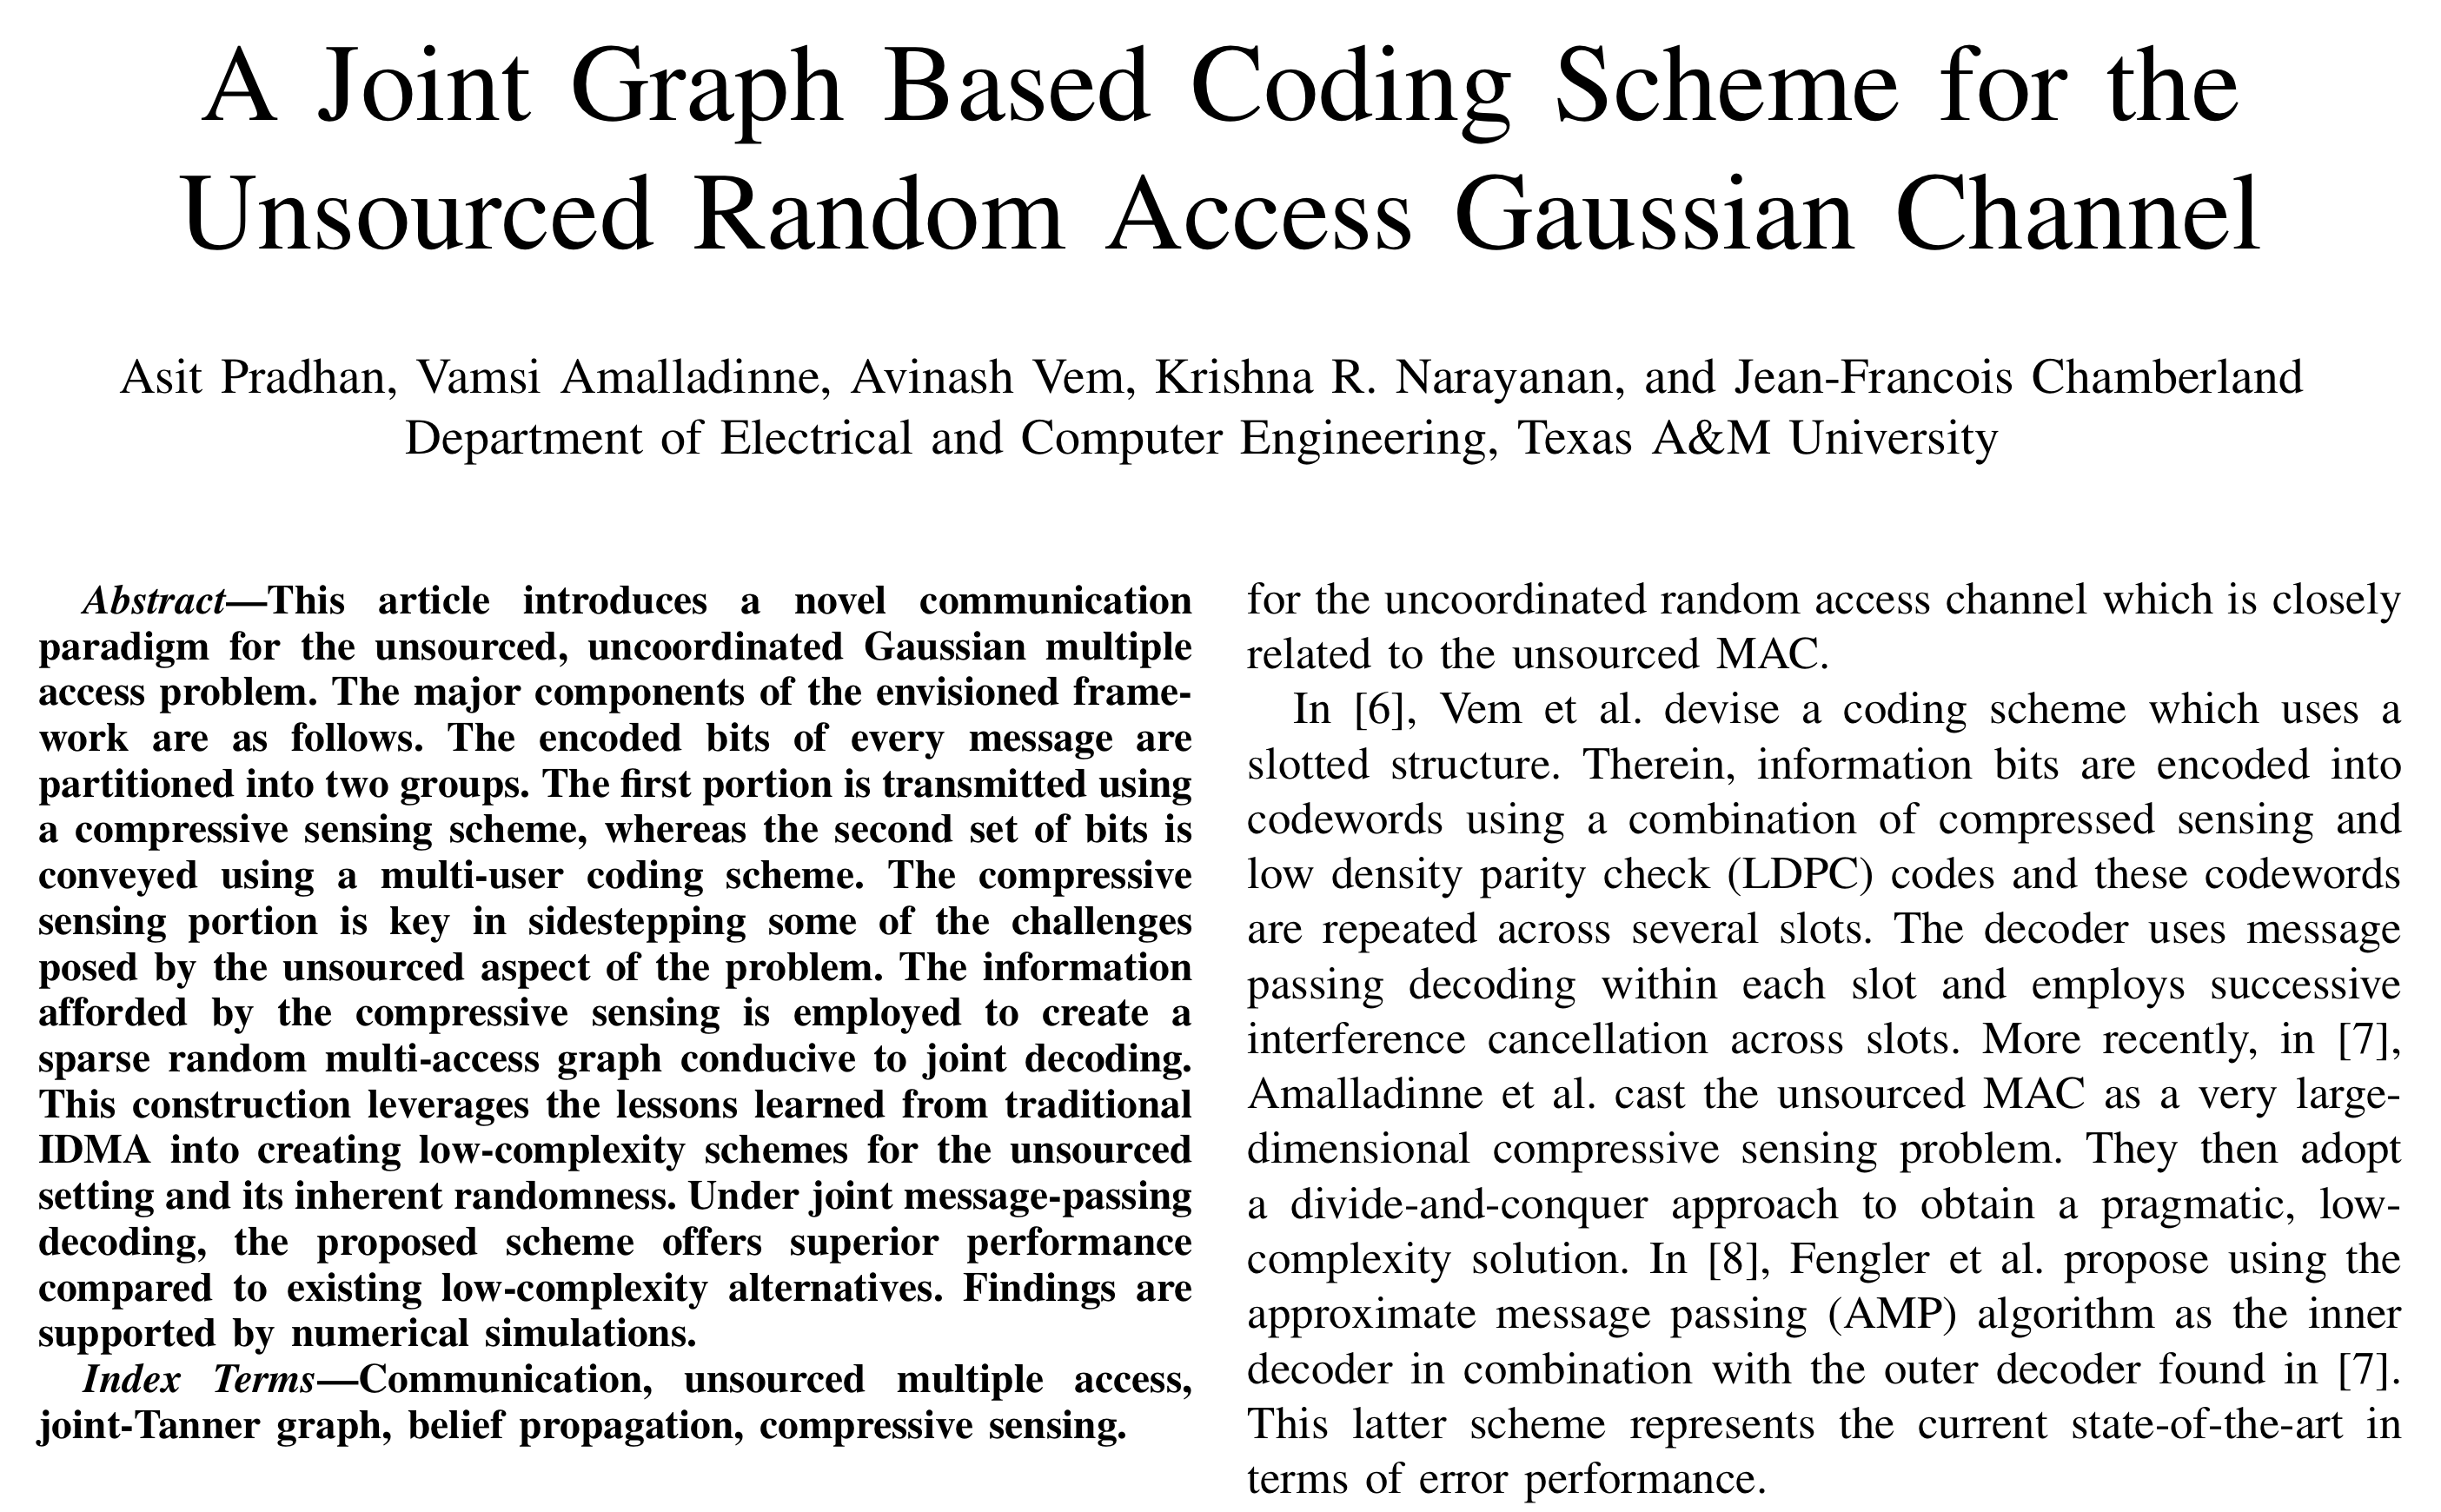
\includegraphics[width=3.5in]{Figures/SparseIDMA.png}};
\end{tikzpicture}
\end{center}
  \begin{itemize}
  \item A. Pradhan, V. Amalladinne, A. Vem, K. Narayanan, JFC
  \item IEEE Global Communications Conference, December 2019
  \end{itemize}
\end{frame}


\begin{frame}
\frametitle{Sparse IDMA}
\begin{center}
\scalebox{0.9}{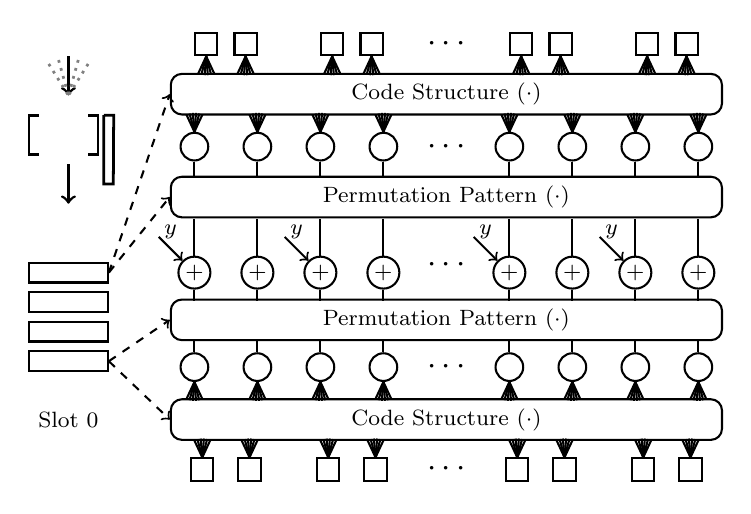
\begin{tikzpicture}
[font=\footnotesize, draw=black, line width=0.75pt,
bitnode/.style={circle,minimum size=10pt,draw=black},
checknode/.style={rectangle,minimum size=8pt,draw=black},
bigPerm/.style={rectangle,draw,minimum width=7cm, minimum height=5mm,rounded corners,draw=black},
sub0/.style={rectangle, draw, inner sep=0pt, minimum width=10mm, minimum height=2.5mm}
]

\def \tcny {2.9}
\def \tvny {1.6}
\def \gmacy {0}
\def \bvny {-1.2}
\def \bcny {-2.5}

\foreach \v in {-2.0} {
  \draw[->, line width=1pt]  (\v,2.75) -- (\v,2.25);
  \draw[dotted, line width=1pt, draw=gray]  (\v-0.25,2.65) -- (\v,2.25);
  \draw[dotted, line width=1pt, draw=gray]  (\v-0.125,2.7) -- (\v,2.25);
  \draw[dotted, line width=1pt, draw=gray]  (\v+0.125,2.7) -- (\v,2.25);
  \draw[dotted, line width=1pt, draw=gray]  (\v+0.25,2.65) -- (\v,2.25);

  \draw[line width=1pt] (\v-0.375,2) -- (\v-0.5,2) -- (\v-0.5,1.5) -- (\v-0.375,1.5);
  \draw[line width=1pt] (\v+0.25,2) -- (\v+0.375,2) -- (\v+0.375,1.5) -- (\v+0.25,1.5);
  \draw[line width=1pt] (\v+0.45,2) -- (\v+0.45,1.125) -- (\v+0.57,1.125) -- (\v+0.575,2) -- (\v+0.45,2);

  \draw[->, line width=1pt]  (\v,1.375) -- (\v,0.875);
}

\foreach \c/\l in {0/1, -0.375/2, -0.75/3, -1.125/4} {
  \node[sub0] (subcs\l) at (-2,\c) {};
}

\foreach \x/\i in {0/1,2/2,5/3,7/4} {
% Top Check Nodes
  \node[checknode] (tbcna\i) at (0.8*\x-0.25, \tcny) {};
  \node[checknode] (tbcnb\i) at (0.8*\x+0.25, \tcny) {};

% Top Variable Nodes
  \node[bitnode] (tvna\i) at (0.8*\x-0.4, \tvny) {};
  \node[bitnode] (tvnb\i) at (0.8*\x+0.4, \tvny) {};

% GMAC Code Symbols
  \node[bitnode,inner sep=1pt] (gmaca\i) at (0.8*\x-0.4, \gmacy) {$+$};
  \node[bitnode,inner sep=1pt] (gmacb\i) at (0.8*\x+0.4, \gmacy) {$+$};

% Bottom Variable Nodes
  \node[bitnode] (bvna\i) at (0.8*\x-0.4, \bvny) {};
  \node[bitnode] (bvnb\i) at (0.8*\x+0.4, \bvny) {};

% Bottom Check Nodes
  \node[checknode] (bcna\i) at (0.8*\x-0.3, \bcny) {};
  \node[checknode] (bcnb\i) at (0.8*\x+0.3, \bcny) {};

% Edges - Set 1
  \foreach \angle in {65,75,85,95,105,115} {
    \draw (tvna\i.north) -- +(\angle:0.24);
    \draw (tvnb\i.north) -- +(\angle:0.24);
    \draw (bcna\i.north) -- +(\angle:0.24);
    \draw (bcnb\i.north) -- +(\angle:0.24);
    }

% Edges - Set 2
  \foreach \angle in {245,255,265,275,285,295} {
    \draw (tbcna\i.south) -- +(\angle:0.24);
    \draw (tbcnb\i.south) -- +(\angle:0.24);
    \draw (bvna\i.south) -- +(\angle:0.24);
    \draw (bvnb\i.south) -- +(\angle:0.24);
    }

  \draw (gmaca\i.south) -- +(0,-0.14);
  \draw (gmacb\i.south) -- +(0,-0.14);
  \draw (gmaca\i.north) -- +(0,0.47);
  \draw (gmacb\i.north) -- +(0,0.46);

  \draw (bvna\i.north) -- +(0,0.15);
  \draw (bvnb\i.north) -- +(0,0.15);
  \draw (tvna\i.south) -- +(0,-0.18);
  \draw (tvnb\i.south) -- +(0,-0.18);

  \draw[<-] (gmaca\i.north west) -- node[midway, above]{$y$} +(-0.3,0.3);
}

  \node at (2.8,\tcny) {\large $\cdots$};
  \node at (2.8,\tvny) {\large $\cdots$};
  \node at (2.8,\gmacy+0.1) {\large $\cdots$};
  \node at (2.8,\bvny) {\large $\cdots$};
  \node at (2.8,\bcny) {\large $\cdots$};

  \node[bigPerm] (tvn2cny) at (2.8,0.4875*\tvny+0.5125*\tcny) {Code Structure $(\cdot)$};
  \node[bigPerm] (tvn2gmacy) at (2.8,0.6*\tvny+0.4*\gmacy) {Permutation Pattern $(\cdot)$};
  \node[bigPerm] (bvn2gmacy) at (2.8,0.5*\gmacy+0.5*\bvny) {Permutation Pattern $(\cdot)$};
  \node[bigPerm] (bvn2cny) at (2.8,0.4875*\bvny+0.5125*\bcny) {Code Structure $(\cdot)$};

  \node (slot0) at (-2,0.4875*\bvny+0.5125*\bcny) {Slot 0};

\draw[->,dashed] (subcs1.east) -- (tvn2cny.west);
\draw[->,dashed] (subcs1.east) -- (tvn2gmacy.west);

\draw[->,dashed] (subcs4.east) -- (bvn2cny.west);
\draw[->,dashed] (subcs4.east) -- (bvn2gmacy.west);
\end{tikzpicture}
}
\end{center}
  \begin{itemize}
  \item Compressed sensing preamble with information bits
  \item Sparse random multi-access graph conducive to joint decoding.
  \end{itemize}
\end{frame}


\begin{frame}
\frametitle{Performance of Unsourced GMAC Schemes}
\begin{center}
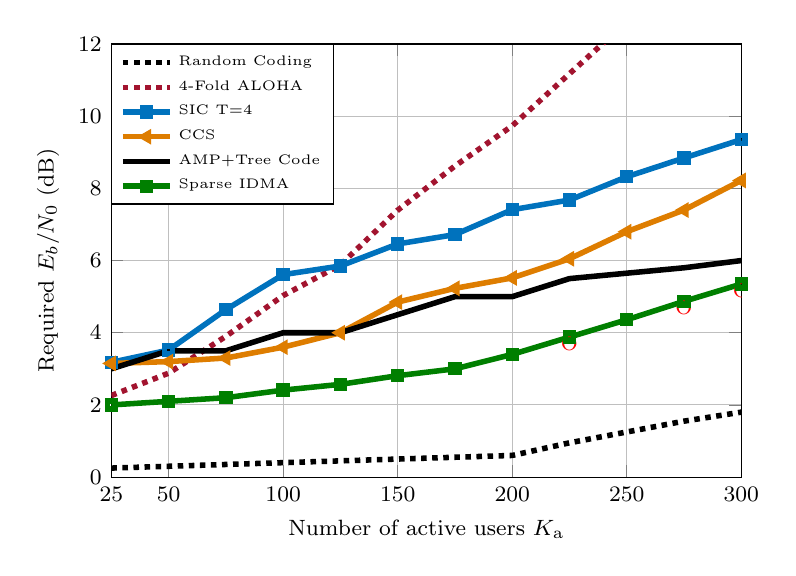
\begin{tikzpicture}
\definecolor{mycolor1}{rgb}{0.63529,0.07843,0.18431}%
\definecolor{mycolor2}{rgb}{0.00000,0.44706,0.74118}%
\definecolor{mycolor3}{rgb}{0.00000,0.49804,0.00000}%
\definecolor{mycolor4}{rgb}{0.87059,0.49020,0.00000}%
\definecolor{mycolor5}{rgb}{0.00000,0.44700,0.74100}%
\definecolor{mycolor6}{rgb}{0.74902,0.00000,0.74902}%

\begin{axis}[%
font=\footnotesize,
width=8cm,
height=5.5cm,
scale only axis,
xmin=25,
xmax=300,
xtick = {25,50,100,...,300},
xlabel={Number of active users $K_{\mathrm{a}}$},
xmajorgrids,
ymin=0,
ymax=12,
ytick = {0,2,...,12},
ylabel={Required $E_b/N_0$ (dB)},
ylabel near ticks,
ymajorgrids,
legend style={font=\tiny, at={(0,1)},anchor=north west, draw=black,fill=white,legend cell align=left}
]

\addplot [color=black,dotted,line width=2.0pt]
  table[row sep=crcr]{
 25	0.25\\
50	0.3\\
75	0.35\\
100	0.4\\
125	0.45\\
150	0.5\\
175	0.55\\
200	0.6\\
225	0.95\\
250	1.25\\
275	1.55\\
300	1.8\\
};
\addlegendentry{Random Coding};

\addplot [color=mycolor1,dotted,line width=2.0pt]
  table[row sep=crcr]{25	2.26\\
50	2.88\\
75	3.9\\
100	5.03\\
125	5.8798\\
150	7.3954\\
175	8.6199\\
200	9.7328\\
225	11.1761\\
250	12.6127\\
275	13.3907\\
300	14.9116\\
};
\addlegendentry{4-Fold ALOHA};

%\addplot [color=mycolor5,dotted,line width=2.0pt]
%  table[row sep=crcr]{25	7.5\\
%35	7.3\\
%50	8.75\\
%100	11.7\\
%150	14.5\\
%200	18\\
%250	21\\
%300	23\\
%};
%\addlegendentry{OP-Exact};

\addplot [color=mycolor2,solid,line width=2.0pt,mark size=1.4pt,mark=square,mark options={solid}]
  table[row sep=crcr]{25	3.18\\
50	3.52\\
75	4.64\\
100	5.61\\
125	5.85\\
150	6.46\\
175	6.72\\
200	7.41\\
225	7.6772\\
250	8.3217\\
275	8.8428\\
300	9.352\\
};
\addlegendentry{SIC T=4};

\addplot [color=mycolor4,solid,line width=2.0pt,mark size=1.3pt,mark=triangle,mark options={solid,rotate=90}]
  table[row sep=crcr]{
  25  3.15\\
50	3.2\\
75	3.3\\
100	3.6\\
125	4\\
150	4.85\\
175	5.23\\
200	5.52\\
225	6.05\\
250	6.8\\
275	7.4\\
300	8.22\\
};
\addlegendentry{CCS};

\addplot [color=black,solid,line width=2.0pt]
  table[row sep=crcr]{
25	3\\
50	3.5\\
75  3.5\\
100	4\\
125	4\\
150 4.5\\
175 5\\
200	5\\
225 5.5
250	5.8\\
275 5.8\\
300	6\\
};
\addlegendentry{AMP+Tree Code};

\addplot [color=mycolor3,solid,line width=2.0pt,mark size=1.4pt,mark=square,mark options={solid}]
  table[row sep=crcr]{
  25  2\\
50	2.1\\
75	2.2\\
100	2.41\\
125	2.57\\
150	2.81\\
175	3\\
200 3.4\\
225 3.88\\
250 4.36\\
275 4.87\\
300 5.35\\
};
\addlegendentry{Sparse IDMA};
\node[] at (axis cs: 300,5.15) {\scriptsize \textcolor{red}{O}};
\node[] at (axis cs: 275,4.69) {\scriptsize \textcolor{red}{O}};
\node[] at (axis cs: 225,3.7) {\scriptsize \textcolor{red}{O}};
%\node[] at (axis cs: 200,4.8) {\scriptsize X};
%\node[] at (axis cs: 200,4.43) {\scriptsize O};
%\addplot [color=black,mark size=2.0pt,only marks,mark=square,mark options={solid}]
%table[row sep=crcr]{
%200 4.43\\
%};
%\node[] at (axis cs: 200,4.43) {\footnotesize O};

%\addplot [color=mycolor6,mark size=6.0pt,only marks,mark=x,mark options={solid},forget plot]
%  table[row sep=crcr]{200	4.8\\
%};
%
%\addplot [color=mycolor5,mark size=5.0pt,only marks,mark=+,mark options={solid},forget plot]
%  table[row sep=crcr]{200	4.43\\
%};

\end{axis}

%\addplot [color=red,solid,line width=2.0pt,mark size=3.5pt,mark=diamond,mark options={solid}]
%  table[row sep=crcr]{25	3.9849\\
%50	5.6396\\
%75	6.2855\\
%100	6.7952\\
%125	7.5262\\
%150	8.3122\\
%175	9.1418\\
%200	10.103\\
%225	11.062\\
%250	12.279\\
%275	13.296\\
%300	14.6648\\
%};
%\addlegendentry{SIC T=2};

%\addplot [color=mycolor3,solid,line width=2.0pt,mark size=2.0pt,mark=+,mark options={solid}]
%  table[row sep=crcr]{25	4.4\\
%50	4.8\\
%75	5.16\\
%100	5.5\\
%125	5.85\\
%150	6.9\\
%175	7.5\\
%200	7.95\\
%225	8.7\\
%250	9.4167\\
%275	10.2773\\
%300	11.37\\
%};
%\addlegendentry{Proposed Scheme, 0 iterations};

\end{tikzpicture}%


\end{center}
\end{frame}


\begin{frame}
\frametitle{Discussion -- Unsourced Multiple Access Channel}

\begin{block}{Summary}
\begin{itemize}
\item Reviewed several frameworks for unsourced multiple access
\item There are close connections between graph-based codes, compressive sensing, and UMAC
\item There remains a gap from information-theoretic results
\item Many theoretical and practical challenges exist
\end{itemize}
\end{block}
\begin{block}{Current Approach}
When carefully designed, single sparse joint Tanner graph that spans across all transmissions offers state-of-the-art performance
\end{block}
\begin{center}
  \begin{tikzpicture}
  \shade[draw=none,
  left color={rgb:red,1;green,2;blue,3},
  right color=frametitle.fg,
  shading angle=60,
  rounded corners,
  blur shadow={shadow blur steps=5}] (-2.25,-0.625) rectangle (2.25,0.625);
  \shade[fill=white, fill opacity=0.1] (-2.25,-0.625) rectangle (2.25,0.625);
  \node at (0,0) {\textcolor{white}{\Large \textbf{Questions?}}};
  \end{tikzpicture}
\end{center}
\end{frame}


\begin{frame}{}
\begin{center}
\scalebox{0.75}{\begin{tikzpicture}[
  font=\scriptsize, >=stealth', line width=1.25pt, line cap=round,
  node/.style={circle, minimum size=3.25mm, inner sep=0pt, draw=black}
]

\node[node] (s1) at (0,3.1) {1};
  \node[node] (s1-1) at (1,3.1) {1};
    \node[node] (s1-1-1) at (2.5,3.1) {1};
      \node[node,label=right:{$(1,1,1,1)$}] (s1-1-1-1) at (5,3.1) {1};
      \node[node,label=right:{$(1,1,1,4)$}] (s1-1-1-4) at (5,-1.5) {3};
    \node[node] (s1-1-3) at (2.5,-0.5) {3};
      \node[node,label=right:{$(1,1,3,1)$}] (s1-1-3-1) at (5,1.9) {3};
      \node[node,label=right:{$(1,1,3,3)$}] (s1-1-3-3) at (5,-0.5) {3};
      \node[node,label=right:{$(1,1,3,4)$}] (s1-1-3-4) at (5,-2.7) {6};
  \node[node] (s1-2) at (1,0.9) {3};
    \node[node] (s1-2-1) at (2.5,2.7) {3};
      \node[node,label=right:{$(1,2,1,1)$}] (s1-2-1-1) at (5,2.7) {3};
      \node[node,label=right:{$(1,2,1,2)$}] (s1-2-1-2) at (5,0.9) {3};
      \node[node,label=right:{$(1,2,1,4)$}] (s1-2-1-4) at (5,-1.9) {6};
    \node[node] (s1-2-2) at (2.5,0.9) {3};
      \node[node,label=right:{$(1,2,2,1)$}] (s1-2-2-1) at (5,2.3) {3};
      \node[node,label=right:{$(1,2,2,2)$}] (s1-2-2-2) at (5,0.5) {3};
      \node[node,label=right:{$(1,2,2,4)$}] (s1-2-2-4) at (5,-2.3) {6};
    \node[node] (s1-2-3) at (2.5,-0.9) {6};
      \node[node,label=right:{$(1,2,3,1)$}] (s1-2-3-1) at (5,1.5) {6};
      \node[node,label=right:{$(1,2,3,2)$}] (s1-2-3-2) at (5,0.1) {6};
      \node[node,label=right:{$(1,2,3,3)$}] (s1-2-3-3) at (5,-0.9) {6};
      \node[node,label=right:{$(1,2,3,4)$}] (s1-2-3-4) at (5,-3.1) {6};

\draw[line width=0.5pt] (s1) -- (s1-1);
  \draw[line width=0.5pt] (s1-1) -- (s1-1-1);
    \draw[line width=0.5pt] (s1-1-1) -- (s1-1-1-1);
    \draw[line width=1.5pt] (s1-1-1) -- (s1-1-1-4);
  \draw[line width=1.5pt] (s1-1) -- (s1-1-3);
    \draw[line width=1.5pt] (s1-1-3) -- (s1-1-3-1);
    \draw[line width=1.5pt] (s1-1-3) -- (s1-1-3-3);
    \draw[line width=3.0pt] (s1-1-3) -- (s1-1-3-4);
\draw[line width=1.5pt] (s1) -- (s1-2);
  \draw[line width=1.5pt] (s1-2) -- (s1-2-1);
    \draw[line width=1.5pt] (s1-2-1) -- (s1-2-1-1);
    \draw[line width=1.5pt] (s1-2-1) -- (s1-2-1-2);
    \draw[line width=3.0pt] (s1-2-1) -- (s1-2-1-4);
  \draw[line width=1.5pt] (s1-2) -- (s1-2-2);
    \draw[line width=1.5pt] (s1-2-2) -- (s1-2-2-1);
    \draw[line width=1.5pt] (s1-2-2) -- (s1-2-2-2);
    \draw[line width=3.0pt] (s1-2-2) -- (s1-2-2-4);
  \draw[line width=3.0pt] (s1-2) -- (s1-2-3);
    \draw[line width=3.0pt] (s1-2-3) -- (s1-2-3-1);
    \draw[line width=3.0pt] (s1-2-3) -- (s1-2-3-2);
    \draw[line width=3.0pt] (s1-2-3) -- (s1-2-3-3);
    \draw[line width=3.0pt] (s1-2-3) -- (s1-2-3-4);

\draw[dashed] (-0.4,3.4) -- (6.8,3.4);
\draw[dashed] (-0.1,1.2) -- (6.5,1.2);
\draw[dashed] (-0.1,-0.2) -- (6.5,-0.2);
\draw[dashed] (-0.1,-1.2) -- (6.5,-1.2);
\draw[dashed] (-0.4,-3.4) -- (6.8,-3.4);

\node[rotate=90] at (-0.4,2.3) {\normalsize level~$1$};
\node[rotate=90] at (-0.4,0.5) {\normalsize level~$2$};
\node[rotate=90] at (-0.4,-0.7) {\normalsize level~$3$};
\node[rotate=90] at (-0.4,-2.3) {\normalsize level~$4$};

\node[rotate=-90] at (6.8,0) {\normalsize $j$-patterns};
\end{tikzpicture}
}
\end{center}
  \begin{center}
  \begin{tikzpicture}
  \shade[draw=none,
  left color={rgb:red,1;green,2;blue,3},
  right color=frametitle.fg,
  shading angle=60,
  rounded corners,
  blur shadow={shadow blur steps=5}] (-2.25,-0.625) rectangle (2.25,0.625);
  \shade[fill=white, fill opacity=0.1] (-2.25,-0.625) rectangle (2.25,0.625);
  \node at (0,0) {\textcolor{white}{\Large \textbf{Thank You!}}};
  \end{tikzpicture}
  \end{center}
\myfootnote{\scriptsize This material is based upon work supported, in part, by NSF under Grant No.~1619085}
\myfootnote{\scriptsize This material is also based upon work support, in part, by Qualcomm Technologies, Inc., through their University Relations Program}
\end{frame}

\begin{frame}
\frametitle{Asynchronous UMAC}
\begin{center}
\begin{tikzpicture}
  \node[scope fading=south] (image) at (0,0) {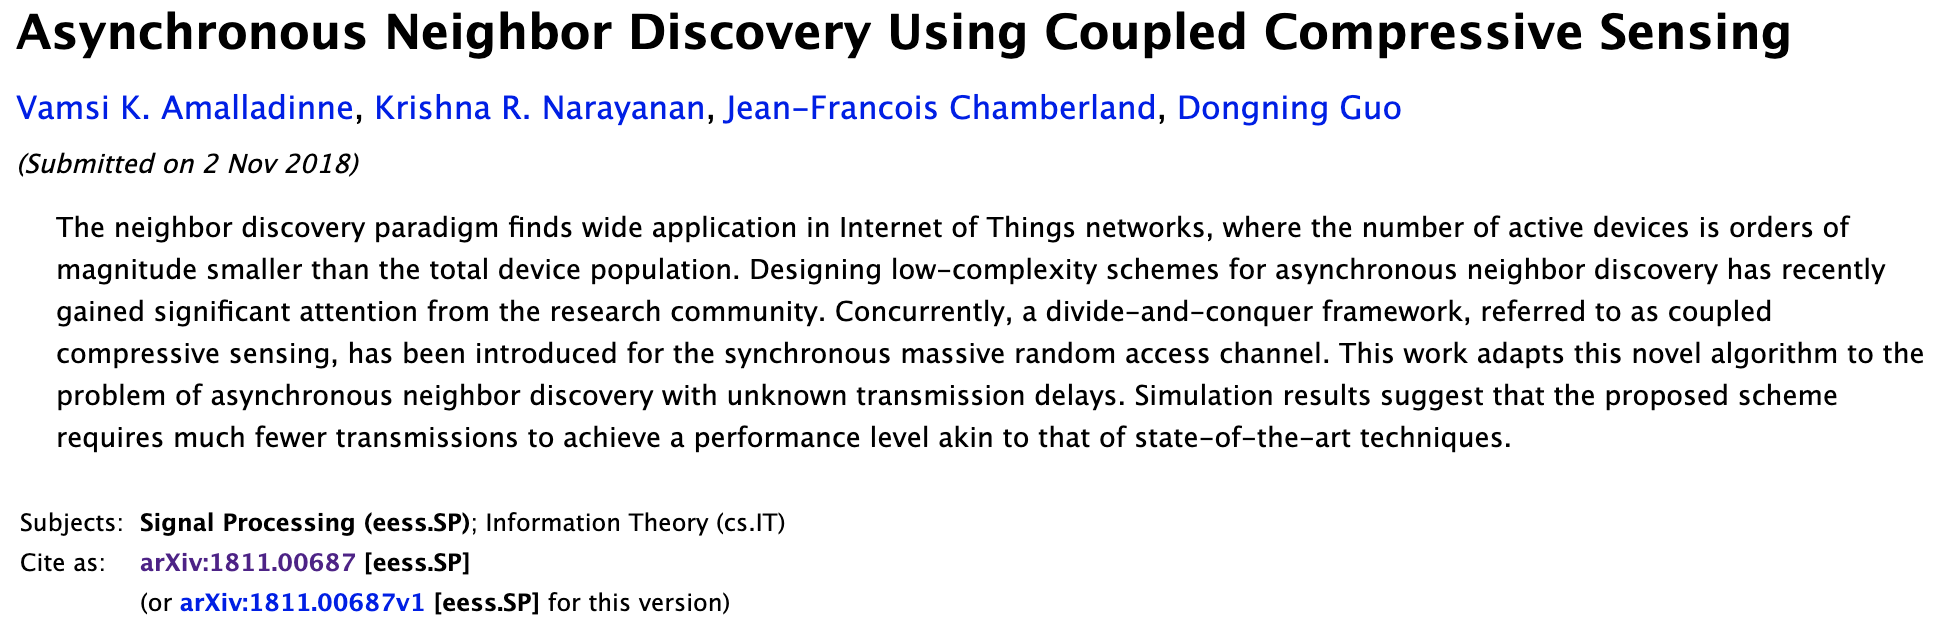
\includegraphics[width=4in]{Figures/ICASSP2019.png}};
\end{tikzpicture}
\end{center}
\vfill
\begin{block}{Building Robust Sensing Matrices}
  \begin{itemize}
  \item Extending CCS framework with low sample complexity
  \item Addressing issues pertaining to asynchrony
  \item Context of neighbor discovery
  \end{itemize}
\end{block}
\end{frame}

\begin{frame}
\frametitle{Dealing with Jitter and Asynchrony}
\begin{center}
  \scalebox{1.25}{
\begin{tikzpicture}
[font=\small, draw=black, line width=0.75pt,
entry0/.style={rectangle, draw, opacity=0.3, fill=lightgray, inner sep=0pt, minimum size=2.5mm},
entry1/.style={rectangle, draw, opacity=0.3, fill=gray, inner sep=0pt, minimum size=2.5mm},
entry00/.style={rectangle, draw, fill=white, inner sep=0pt, minimum size=2.5mm},
entry11/.style={rectangle, draw, fill=darkgray!90, inner sep=0pt, minimum size=2.5mm},
entry2/.style={rectangle, draw, fill=blue, inner sep=0pt, minimum size=2.5mm},
noentry/.style={rectangle, inner sep=0pt, minimum size=2.5mm},
symbol0/.style={rectangle, draw, fill=white, inner sep=0pt, minimum size=2.5mm},
symbol1/.style={rectangle, draw, fill=blue!50, inner sep=0pt, minimum size=2.5mm}]

\node[noentry] (m0000) at (0.00,0) {};
\node[entry11] (m0100) at (0.25,0) {};
\node[noentry] (m0200) at (0.50,0) {};
\node[entry00] (m0300) at (0.75,0) {};
\node[noentry] (m0400) at (1.00,0) {};
\node[noentry] (m0500) at (1.25,0) {};
\node[noentry] (m0600) at (1.50,0) {};
\node[noentry] (m0700) at (1.75,0) {};
\node[noentry] (m0800) at (2.00,0) {};
\node[noentry] (m0900) at (2.25,0) {};
\node[entry00] (m1000) at (2.50,0) {};
\node[noentry] (m1100) at (2.75,0) {};

\node[entry0] (m0001) at (0.00,0.25) {};
\node[entry11] (m0101) at (0.25,0.25) {};
\node[entry0] (m0201) at (0.50,0.25) {};
\node[entry11] (m0301) at (0.75,0.25) {};
\node[entry0] (m0401) at (1.00,0.25) {};
\node[entry0] (m0501) at (1.25,0.25) {};
\node[entry00] (m0601) at (1.50,0.25) {};
\node[entry1] (m0701) at (1.75,0.25) {};
\node[entry1] (m0801) at (2.00,0.25) {};
\node[entry1] (m0901) at (2.25,0.25) {};
\node[entry00] (m1001) at (2.50,0.25) {};
\node[entry0] (m1101) at (2.75,0.25) {};

\node[entry0] (m0002) at (0.00,0.50) {};
\node[entry00] (m0102) at (0.25,0.50) {};
\node[entry1] (m0202) at (0.50,0.50) {};
\node[entry11] (m0302) at (0.75,0.50) {};
\node[entry0] (m0402) at (1.00,0.50) {};
\node[entry1] (m0502) at (1.25,0.50) {};
\node[entry00] (m0602) at (1.50,0.50) {};
\node[entry1] (m0702) at (1.75,0.50) {};
\node[entry1] (m0802) at (2.00,0.50) {};
\node[entry0] (m0902) at (2.25,0.50) {};
\node[entry11] (m1002) at (2.50,0.50) {};
\node[entry0] (m1102) at (2.75,0.50) {};

\node[entry0] (m0003) at (0.00,0.75) {};
\node[entry00] (m0103) at (0.25,0.75) {};
\node[entry0] (m0203) at (0.50,0.75) {};
\node[entry00] (m0303) at (0.75,0.75) {};
\node[entry1] (m0403) at (1.00,0.75) {};
\node[entry1] (m0503) at (1.25,0.75) {};
\node[entry11] (m0603) at (1.50,0.75) {};
\node[entry0] (m0703) at (1.75,0.75) {};
\node[entry1] (m0803) at (2.00,0.75) {};
\node[entry0] (m0903) at (2.25,0.75) {};
\node[entry11] (m1003) at (2.50,0.75) {};
\node[entry0] (m1103) at (2.75,0.75) {};

\node[entry1] (m0004) at (0.00,1.00) {};
\node[entry11] (m0104) at (0.25,1.00) {};
\node[entry0] (m0204) at (0.50,1.00) {};
\node[entry00] (m0304) at (0.75,1.00) {};
\node[entry0] (m0404) at (1.00,1.00) {};
\node[entry0] (m0504) at (1.25,1.00) {};
\node[entry00] (m0604) at (1.50,1.00) {};
\node[entry0] (m0704) at (1.75,1.00) {};
\node[entry0] (m0804) at (2.00,1.00) {};
\node[entry1] (m0904) at (2.25,1.00) {};
\node[entry00] (m1004) at (2.50,1.00) {};
\node[entry0] (m1104) at (2.75,1.00) {};

\node[entry0] (m0005) at (0.00,1.25) {};
\node[entry00] (m0105) at (0.25,1.25) {};
\node[entry1] (m0205) at (0.50,1.25) {};
\node[entry11] (m0305) at (0.75,1.25) {};
\node[entry0] (m0405) at (1.00,1.25) {};
\node[entry1] (m0505) at (1.25,1.25) {};
\node[entry11] (m0605) at (1.50,1.25) {};
\node[entry1] (m0705) at (1.75,1.25) {};
\node[entry1] (m0805) at (2.00,1.25) {};
\node[entry0] (m0905) at (2.25,1.25) {};
\node[entry00] (m1005) at (2.50,1.25) {};
\node[entry0] (m1105) at (2.75,1.25) {};

\node[entry0] (m0006) at (0.00,1.5) {};
\node[noentry] (m0106) at (0.25,1.5) {};
\node[entry0] (m0206) at (0.50,1.5) {};
\node[noentry] (m0306) at (0.75,1.5) {};
\node[entry0] (m0406) at (1.00,1.5) {};
\node[entry1] (m0506) at (1.25,1.5) {};
\node[entry11] (m0606) at (1.50,1.5) {};
\node[entry0] (m0706) at (1.75,1.5) {};
\node[entry1] (m0806) at (2.00,1.5) {};
\node[entry0] (m0906) at (2.25,1.5) {};
\node[noentry] (m1006) at (2.50,1.5) {};
\node[entry1] (m1106) at (2.75,1.5) {};


\node[symbol0] (s1) at (3.5,-1.25) {};
\node[symbol1] (s2) at (3.5,-1.00) {};
\node[symbol0] (s3) at (3.5,-0.75) {};
\node[symbol1] (s4) at (3.5,-0.50) {};
\node[symbol0] (s5) at (3.5,-0.25) {};
\node[symbol0] (s6) at (3.5,0.00) {};
\node[symbol1] (s7) at (3.5,0.25) {};
\node[symbol0] (s8) at (3.5,0.50) {};
\node[symbol0] (s9) at (3.5,0.75) {};
\node[symbol0] (s10) at (3.5,1.00) {};
\node[symbol1] (s11) at (3.5,1.25) {};
\node[symbol0] (s12) at (3.5,1.5) {};

\node (equal) at (4.25,0.75) {\Large =};

\node[entry2,fill=blue!20] (y00) at (5,0.00) {};
\node[entry2,fill=blue!40] (y00) at (5,0.25) {};
\node[entry2,fill=blue!40] (y01) at (5,0.50) {};
\node[entry2,fill=blue!20] (y02) at (5,0.75) {};
\node[entry2,fill=blue!20] (y03) at (5,1.00) {};
\node[entry2,fill=blue!40] (y04) at (5,1.25) {};
\node[entry2,fill=blue!20] (y05) at (5,1.50) {};


\node[anchor=west] (samplingmatrix) at (-0.15,-0.75) {Distorted Matrix};
\node[rotate=-90] (ageindices) at (3.95,-0.9) {Indices};
\node[rotate=-90] (receivedsignal) at (5.5,0.6) {Received Signal};
\end{tikzpicture}}

\end{center}
\begin{block}{Asynchronous Signals}
  \begin{itemize}
  \item $\vec{y} = \tilde{A} \tilde{\vec{x}} + \vec{z}$ with  $\|\vec{x}\|_0 = K$
  \item $\tilde{A} \in \mathbb{C}^{(n+\mathcal{T}) \times 2^B}$ unknown due to unknown random delays
  \item Max delay $\mathcal{T}$ known to the decoder
  \end{itemize}
\end{block}
\end{frame}


\begin{frame}
\frametitle{Expanded Codebook through Sensing Matrix}
\begin{center}
  \begin{tikzpicture}
[font=\small, draw=black, line width=0.75pt,
entry0/.style={rectangle, draw, opacity=0.3, fill=lightgray, inner sep=0pt, minimum size=2.5mm},
entry1/.style={rectangle, draw, opacity=0.3, fill=gray, inner sep=0pt, minimum size=2.5mm},
entry00/.style={rectangle, draw, fill=white, inner sep=0pt, minimum size=2.5mm},
entry11/.style={rectangle, draw, fill=darkgray!90, inner sep=0pt, minimum size=2.5mm},
entry2/.style={rectangle, draw, fill=blue, inner sep=0pt, minimum size=2.5mm},
noentry/.style={rectangle, draw, opacity=0.3, fill=lightgray!50!gray!50, inner sep=0pt, minimum size=2.5mm},
symbol0/.style={rectangle, draw, fill=white, inner sep=0pt, minimum size=2.5mm},
symbol1/.style={rectangle, draw, fill=blue!50, inner sep=0pt, minimum size=2.5mm}]

\node[noentry] (m0000) at (0.00,0) {};
\node[entry0] (m0100) at (0.25,0) {};
\node[noentry] (m0200) at (0.50,0) {};
\node[entry11] (m0300) at (0.75,0) {};
\node[noentry] (m0400) at (1.00,0) {};
\node[entry0] (m0500) at (1.25,0) {};
\node[noentry] (m0600) at (1.50,0) {};
\node[entry00] (m0700) at (1.75,0) {};
\node[noentry] (m0800) at (2.00,0) {};
\node[entry0] (m0900) at (2.25,0) {};
\node[noentry] (m1000) at (2.50,0) {};
\node[entry0] (m1100) at (2.75,0) {};
\node[noentry] (m1200) at (3.00,0) {};
\node[entry0] (m1300) at (3.25,0) {};
\node[noentry] (m1400) at (3.50,0) {};
\node[entry1] (m1500) at (3.75,0) {};
\node[noentry] (m1600) at (4.00,0) {};
\node[entry1] (m1700) at (4.25,0) {};
\node[noentry] (m1800) at (4.50,0) {};
\node[entry1] (m1900) at (4.75,0) {};
\node[noentry] (m2000) at (5.00,0) {};
\node[entry00] (m2100) at (5.25,0) {};
\node[noentry] (m2200) at (5.50,0) {};
\node[entry0] (m2300) at (5.75,0) {};

\node[entry0] (m0001) at (0.00,0.25) {};
\node[entry0] (m0101) at (0.25,0.25) {};
\node[entry1] (m0201) at (0.50,0.25) {};
\node[entry11] (m0301) at (0.75,0.25) {};
\node[entry0] (m0401) at (1.00,0.25) {};
\node[entry1] (m0501) at (1.25,0.25) {};
\node[entry0] (m0601) at (1.50,0.25) {};
\node[entry11] (m0701) at (1.75,0.25) {};
\node[entry0] (m0801) at (2.00,0.25) {};
\node[entry0] (m0901) at (2.25,0.25) {};
\node[entry0] (m1001) at (2.50,0.25) {};
\node[entry1] (m1101) at (2.75,0.25) {};
\node[entry00] (m1201) at (3.00,0.25) {};
\node[entry0] (m1301) at (3.25,0.25) {};
\node[entry1] (m1401) at (3.50,0.25) {};
\node[entry1] (m1501) at (3.75,0.25) {};
\node[entry1] (m1601) at (4.00,0.25) {};
\node[entry1] (m1701) at (4.25,0.25) {};
\node[entry1] (m1801) at (4.50,0.25) {};
\node[entry0] (m1901) at (4.75,0.25) {};
\node[entry0] (m2001) at (5.00,0.25) {};
\node[entry00] (m2101) at (5.25,0.25) {};
\node[entry0] (m2201) at (5.50,0.25) {};
\node[entry0] (m2301) at (5.75,0.25) {};

\node[entry0] (m0002) at (0.00,0.50) {};
\node[entry0] (m0102) at (0.25,0.50) {};
\node[entry1] (m0202) at (0.50,0.50) {};
\node[entry00] (m0302) at (0.75,0.50) {};
\node[entry1] (m0402) at (1.00,0.50) {};
\node[entry0] (m0502) at (1.25,0.50) {};
\node[entry1] (m0602) at (1.50,0.50) {};
\node[entry11] (m0702) at (1.75,0.50) {};
\node[entry0] (m0802) at (2.00,0.50) {};
\node[entry1] (m0902) at (2.25,0.50) {};
\node[entry1] (m1002) at (2.50,0.50) {};
\node[entry0] (m1102) at (2.75,0.50) {};
\node[entry00] (m1202) at (3.00,0.50) {};
\node[entry1] (m1302) at (3.25,0.50) {};
\node[entry1] (m1402) at (3.50,0.50) {};
\node[entry0] (m1502) at (3.75,0.50) {};
\node[entry1] (m1602) at (4.00,0.50) {};
\node[entry1] (m1702) at (4.25,0.50) {};
\node[entry0] (m1802) at (4.50,0.50) {};
\node[entry0] (m1902) at (4.75,0.50) {};
\node[entry0] (m2002) at (5.00,0.50) {};
\node[entry11] (m2102) at (5.25,0.50) {};
\node[entry0] (m2202) at (5.50,0.50) {};
\node[entry0] (m2302) at (5.75,0.50) {};

\node[entry0] (m0003) at (0.00,0.75) {};
\node[entry0] (m0103) at (0.25,0.75) {};
\node[entry0] (m0203) at (0.50,0.75) {};
\node[entry00] (m0303) at (0.75,0.75) {};
\node[entry0] (m0403) at (1.00,0.75) {};
\node[entry0] (m0503) at (1.25,0.75) {};
\node[entry1] (m0603) at (1.50,0.75) {};
\node[entry00] (m0703) at (1.75,0.75) {};
\node[entry1] (m0803) at (2.00,0.75) {};
\node[entry0] (m0903) at (2.25,0.75) {};
\node[entry1] (m1003) at (2.50,0.75) {};
\node[entry0] (m1103) at (2.75,0.75) {};
\node[entry11] (m1203) at (3.00,0.75) {};
\node[entry0] (m1303) at (3.25,0.75) {};
\node[entry0] (m1403) at (3.50,0.75) {};
\node[entry0] (m1503) at (3.75,0.75) {};
\node[entry1] (m1603) at (4.00,0.75) {};
\node[entry0] (m1703) at (4.25,0.75) {};
\node[entry0] (m1803) at (4.50,0.75) {};
\node[entry1] (m1903) at (4.75,0.75) {};
\node[entry1] (m2003) at (5.00,0.75) {};
\node[entry11] (m2103) at (5.25,0.75) {};
\node[entry0] (m2203) at (5.50,0.75) {};
\node[entry0] (m2303) at (5.75,0.75) {};

\node[entry1] (m0004) at (0.00,1.00) {};
\node[entry0] (m0104) at (0.25,1.00) {};
\node[entry0] (m0204) at (0.50,1.00) {};
\node[entry11] (m0304) at (0.75,1.00) {};
\node[entry0] (m0404) at (1.00,1.00) {};
\node[entry1] (m0504) at (1.25,1.00) {};
\node[entry0] (m0604) at (1.50,1.00) {};
\node[entry00] (m0704) at (1.75,1.00) {};
\node[entry0] (m0804) at (2.00,1.00) {};
\node[entry0] (m0904) at (2.25,1.00) {};
\node[entry0] (m1004) at (2.50,1.00) {};
\node[entry1] (m1104) at (2.75,1.00) {};
\node[entry00] (m1204) at (3.00,1.00) {};
\node[entry1] (m1304) at (3.25,1.00) {};
\node[entry0] (m1404) at (3.50,1.00) {};
\node[entry1] (m1504) at (3.75,1.00) {};
\node[entry0] (m1604) at (4.00,1.00) {};
\node[entry1] (m1704) at (4.25,1.00) {};
\node[entry1] (m1804) at (4.50,1.00) {};
\node[entry0] (m1904) at (4.75,1.00) {};
\node[entry1] (m2004) at (5.00,1.00) {};
\node[entry00] (m2104) at (5.25,1.00) {};
\node[entry0] (m2204) at (5.50,1.00) {};
\node[entry0] (m2304) at (5.75,1.00) {};

\node[entry0] (m0005) at (0.00,1.25) {};
\node[entry0] (m0105) at (0.25,1.25) {};
\node[entry1] (m0205) at (0.50,1.25) {};
\node[entry00] (m0305) at (0.75,1.25) {};
\node[entry1] (m0405) at (1.00,1.25) {};
\node[entry0] (m0505) at (1.25,1.25) {};
\node[entry0] (m0605) at (1.50,1.25) {};
\node[entry11] (m0705) at (1.75,1.25) {};
\node[entry0] (m0805) at (2.00,1.25) {};
\node[entry0] (m0905) at (2.25,1.25) {};
\node[entry1] (m1005) at (2.50,1.25) {};
\node[entry1] (m1105) at (2.75,1.25) {};
\node[entry11] (m1205) at (3.00,1.25) {};
\node[entry1] (m1305) at (3.25,1.25) {};
\node[entry1] (m1405) at (3.50,1.25) {};
\node[entry0] (m1505) at (3.75,1.25) {};
\node[entry1] (m1605) at (4.00,1.25) {};
\node[entry1] (m1705) at (4.25,1.25) {};
\node[entry0] (m1805) at (4.50,1.25) {};
\node[entry0] (m1905) at (4.75,1.25) {};
\node[entry0] (m2005) at (5.00,1.25) {};
\node[entry00] (m2105) at (5.25,1.25) {};
\node[entry0] (m2205) at (5.50,1.25) {};
\node[entry1] (m2305) at (5.75,1.25) {};

\node[entry0] (m0006) at (0.00,1.50) {};
\node[noentry] (m0106) at (0.25,1.50) {};
\node[entry0] (m0206) at (0.50,1.50) {};
\node[noentry] (m0306) at (0.75,1.50) {};
\node[entry0] (m0406) at (1.00,1.50) {};
\node[noentry] (m0506) at (1.25,1.50) {};
\node[entry1] (m0606) at (1.50,1.50) {};
\node[noentry] (m0706) at (1.75,1.50) {};
\node[entry0] (m0806) at (2.00,1.50) {};
\node[noentry] (m0906) at (2.25,1.50) {};
\node[entry1] (m1006) at (2.50,1.50) {};
\node[noentry] (m1106) at (2.75,1.50) {};
\node[entry11] (m1206) at (3.00,1.50) {};
\node[noentry] (m1306) at (3.25,1.50) {};
\node[entry0] (m1406) at (3.50,1.50) {};
\node[noentry] (m1506) at (3.75,1.50) {};
\node[entry1] (m1606) at (4.00,1.50) {};
\node[noentry] (m1706) at (4.25,1.50) {};
\node[entry0] (m1806) at (4.50,1.50) {};
\node[noentry] (m1906) at (4.75,1.50) {};
\node[entry0] (m2006) at (5.00,1.50) {};
\node[noentry] (m2106) at (5.25,1.50) {};
\node[entry1] (m2206) at (5.50,1.50) {};
\node[noentry] (m2306) at (5.75,1.50) {};

\node (equal) at (7.25,0.75) {\Large =};

\node[symbol0] (s01) at (6.5,-4.25) {};
\node[symbol0] (s02) at (6.5,-4.00) {};
\node[symbol1] (s03) at (6.5,-3.75) {};
\node[symbol0] (s04) at (6.5,-3.50) {};
\node[symbol0] (s05) at (6.5,-3.25) {};
\node[symbol0] (s06) at (6.5,-3.00) {};
\node[symbol1] (s07) at (6.5,-2.75) {};
\node[symbol0] (s08) at (6.5,-2.50) {};
\node[symbol0] (s09) at (6.5,-2.25) {};
\node[symbol0] (s10) at (6.5,-2.00) {};
\node[symbol0] (s11) at (6.5,-1.75) {};
\node[symbol0] (s12) at (6.5,-1.50) {};
\node[symbol1] (s13) at (6.5,-1.25) {};
\node[symbol0] (s14) at (6.5,-1.00) {};
\node[symbol0] (s15) at (6.5,-0.75) {};
\node[symbol0] (s16) at (6.5,-0.50) {};
\node[symbol0] (s17) at (6.5,-0.25) {};
\node[symbol0] (s18) at (6.5,0.00) {};
\node[symbol0] (s19) at (6.5,0.25) {};
\node[symbol0] (s20) at (6.5,0.50) {};
\node[symbol0] (s21) at (6.5,0.75) {};
\node[symbol1] (s22) at (6.5,1.00) {};
\node[symbol0] (s23) at (6.5,1.25) {};
\node[symbol0] (s24) at (6.5,1.50) {};

\node[entry2,fill=blue!20] (y00) at (8,0.00) {};
\node[entry2,fill=blue!40] (y01) at (8,0.25) {};
\node[entry2,fill=blue!40] (y02) at (8,0.50) {};
\node[entry2,fill=blue!20] (y03) at (8,0.75) {};
\node[entry2,fill=blue!20] (y04) at (8,1.00) {};
\node[entry2,fill=blue!40] (y05) at (8,1.25) {};
\node[entry2,fill=blue!20] (y06) at (8,1.50) {};

\node[anchor=west] (samplingmatrix) at (0.5,-1) {Expanded Codebook $\mathbf{A}$};
\node[anchor=west] (vector) at (0.5,-1.5) {$(n+\mathcal{T})\times2^B(\mathcal{T}+1)$ matrix};
\node[anchor=west] (framework1) at (0.5,-2) {Accounts for all possible delays};
\node[anchor=west] (framework2) at (0.5,-2.5) {$K$ out of $2^B(\mathcal{T}+1)$ sparse};

\node[rotate=-90] (ageindices) at (7,-0.75) {Message Indices};
\node[rotate=-90] (receivedsignal) at (8.5,0.6) {Received Signal};

\end{tikzpicture}

\end{center}
  \begin{itemize}
  \item Computational complexity of CS solvers: $\mathcal{O}(\mathrm{poly}(2^B(\mathcal{T}+1)))$
  \end{itemize}
\end{frame}


\begin{frame}
\frametitle{Hybrid Methods and Alternatives}
\begin{block}{Intermittent CCS}
\begin{columns}
\column{.48\textwidth}
  \begin{center}
  \scalebox{1.0}{\begin{tikzpicture}
[font=\footnotesize, draw=black, line width=0.75pt,
fragment/.style={circle, draw, inner sep=0pt}]

\node[fragment,minimum size=2.5mm] (x0y0) at (0, 2) {};
\foreach \y in {0, ..., 4} {
    \node[fragment,minimum size=2mm] (x1y\y) at (1, \y) {}
        edge[dashed] (x0y0);
}
\draw (x0y0) -- (x1y4);
\draw (x0y0) -- (x1y1);

\foreach \y/\p in {51/2.4, 52/2.8, 53/3.2,  54/3.6, 55/4.0} {
    \node[fragment,minimum size=1.5mm] (x2y\y) at (2, \p) {}
        edge[dashed] (x1y4);
}
\draw (x1y4) -- (x2y52);

\foreach \y/\p in {21/0.2, 22/0.6, 23/1.0,  24/1.4, 25/1.8} {
    \node[fragment,minimum size=1.5mm] (x2y\y) at (2, \p) {}
        edge[dashed] (x1y1);
}
\draw (x1y1) -- (x2y24);
\draw (x1y1) -- (x2y21);

\foreach \y/\p in {421/3.2, 422/3.4, 423/3.6,  424/3.8, 425/4.0} {
    \node[fragment,minimum size=1mm] (x3y\y) at (3, \p) {}
        edge[dashed] (x2y52);
}

\foreach \y/\p in {241/1.6, 242/1.8, 243/2.0,  244/2.2, 245/2.4} {
    \node[fragment,minimum size=1mm] (x3y\y) at (3, \p) {}
        edge[dashed] (x2y24);
}
\draw (x2y24) -- (x3y241);
\draw (x2y24) -- (x3y245);

\foreach \y/\p in {211/0.0, 212/0.2, 213/0.4,  214/0.6, 215/0.8} {
    \node[fragment,minimum size=1mm] (x3y\y) at (3, \p) {}
        edge[dashed] (x2y21);
}

\foreach \y/\p in {2451/2.2, 2452/2.4, 2453/2.6,  2454/2.8, 2455/3.0} {
    \node[fragment,minimum size=0.5mm] (x4y\y) at (4, \p) {}
        edge[dashed] (x3y245);
}
\draw (x3y245) -- (x4y2454);

\foreach \y/\p in {2411/1.0, 2412/1.2, 2413/1.4,  2414/1.6, 2415/1.8} {
    \node[fragment,minimum size=0.5mm] (x4y\y) at (4, \p) {}
        edge[dashed] (x3y241);
}

\end{tikzpicture}}
  \end{center}
\column{.48\textwidth}
  \begin{center}
  \scalebox{1.0}{\begin{tikzpicture}
[font=\footnotesize, draw=black, line width=0.75pt,
fragment/.style={circle, draw, inner sep=0pt, minimum size=1mm}]

\node[fragment,minimum size=1mm] (x0y0) at (0, 2) {};

\foreach \y in {0, ..., 4} {
    \node[fragment] (x1y\y) at (1, -0.2+1.1*\y) {}
        edge[densely dashed] (x0y0);
}
\draw (x0y0) -- (x1y0);
\draw (x0y0) -- (x1y3);

\foreach \y in {0, ..., 4} {
    \node[fragment] (x2ys\y) at (2, 1.6+0.2*\y) {}
        edge[dotted] (x0y0);
}
\draw (x0y0) -- (x2ys4);
\foreach \y in {0, ..., 4} {
    \node[fragment] (x2y0\y) at (2, -0.2+0.2*\y) {}
            edge[densely dashed] (x1y0);
}
\draw (x1y0) -- (x2y01);
\foreach \y in {0, ..., 4} {
    \node[fragment] (x2y3\y) at (2, 3.4+0.2*\y) {}
            edge[densely dashed] (x1y3);
}


\foreach \y in {0, ..., 4} {
        \node[fragment] (x3y01\y) at (3, -0.2+0.2*\y) {}
            edge[densely dashed] (x2y01);
}
\draw (x2y01) -- (x3y010);
\foreach \y in {0, ..., 4} {
        \node[fragment] (x3y0s\y) at (3, 1+0.2*\y) {}
            edge[dotted] (x1y0);
}
\foreach \y in {0, ..., 4} {
        \node[fragment] (x3ys4\y) at (3, 2.2+.2*\y) {}
            edge[densely dashed] (x2ys4);
}
\foreach \y in {0, ..., 4} {
        \node[fragment] (x3y3s\y) at (3, 3.4+0.2*\y) {}
            edge[dotted] (x1y3);
}
\draw (x1y3) -- (x3y3s0);

\foreach \y in {0, ..., 4} {
        \node[fragment] (x4y010\y) at (4, -0.2+0.2*\y) {}
            edge[densely dashed] (x3y010);
}
\foreach \y in {0, ..., 4} {
        \node[fragment] (x4y01s\y) at (4, 1+0.2*\y) {}
            edge[dotted] (x2y01);
}
\draw (x2y01) -- (x4y01s3);
\foreach \y in {0, ..., 4} {
        \node[fragment] (x4ys4s\y) at (4, 2.2+.2*\y) {}
            edge[dotted] (x2ys4);
}
\foreach \y in {0, ..., 4} {
        \node[fragment] (x4y3s2\y) at (4, 3.4+0.2*\y) {}
            edge[densely dashed] (x3y3s0);
}

\end{tikzpicture}
}
  \end{center}
\end{columns}
\end{block}
\begin{itemize}
\item Trading off flexibility and complexity
\end{itemize}
\end{frame}

\end{document}


%\begin{frame}
%\frametitle{Example -- Traditional Fountain Codes}
%\begin{columns}
%\column{.48\textwidth}
%\begin{center}
%  \scalebox{0.55}{\begin{tikzpicture}
[draw=black, line width=1.5pt, >=stealth',
entry1/.style={rectangle, draw, fill=gray, inner sep=0pt, minimum size=5mm},
entry0/.style={rectangle, draw, inner sep=0pt, minimum size=5mm},
symbol/.style={rectangle, draw, fill=green!40, inner sep=0pt, minimum size=5mm}]

\node[entry0] (m00) at (0,0) {};
\node[entry1] (m01) at (0.5,0) {};
\node[entry0] (m02) at (1,0) {};
\node[entry0] (m03) at (1.5,0) {};
\node[entry1] (m04) at (2,0) {};
\node[entry0] (m05) at (2.5,0) {};
\node[entry0] (m06) at (3,0) {};
\node[entry0] (m07) at (3.5,0) {};
\node[entry0] (m08) at (4,0) {};
\node[entry0] (m09) at (4.5,0) {};

\node[entry0] (m00) at (0,0.5) {};
\node[entry1] (m11) at (0.5,0.5) {};
\node[entry0] (m12) at (1,0.5) {};
\node[entry0] (m13) at (1.5,0.5) {};
\node[entry0] (m14) at (2,0.5) {};
\node[entry1] (m15) at (2.5,0.5) {};
\node[entry0] (m16) at (3,0.5) {};
\node[entry0] (m17) at (3.5,0.5) {};
\node[entry0] (m18) at (4,0.5) {};
\node[entry0] (m19) at (4.5,0.5) {};

\node[entry0] (m20) at (0,1) {};
\node[entry0] (m21) at (0.5,1) {};
\node[entry0] (m22) at (1,1) {};
\node[entry0] (m23) at (1.5,1) {};
\node[entry0] (m24) at (2,1) {};
\node[entry0] (m25) at (2.5,1) {};
\node[entry1] (m26) at (3,1) {};
\node[entry0] (m27) at (3.5,1) {};
\node[entry0] (m28) at (4,1) {};
\node[entry0] (m29) at (4.5,1) {};

\node[entry0] (m30) at (0,1.5) {};
\node[entry0] (m31) at (0.5,1.5) {};
\node[entry0] (m32) at (1,1.5) {};
\node[entry0] (m33) at (1.5,1.5) {};
\node[entry0] (m34) at (2,1.5) {};
\node[entry1] (m35) at (2.5,1.5) {};
\node[entry0] (m36) at (3,1.5) {};
\node[entry1] (m37) at (3.5,1.5) {};
\node[entry0] (m38) at (4,1.5) {};
\node[entry1] (m39) at (4.5,1.5) {};

\node[entry0] (m40) at (0,2) {};
\node[entry1] (m41) at (0.5,2) {};
\node[entry0] (m42) at (1,2) {};
\node[entry1] (m43) at (1.5,2) {};
\node[entry0] (m44) at (2,2) {};
\node[entry0] (m45) at (2.5,2) {};
\node[entry0] (m46) at (3,2) {};
\node[entry0] (m47) at (3.5,2) {};
\node[entry0] (m48) at (4,2) {};
\node[entry0] (m49) at (4.5,2) {};

\node[entry0] (m50) at (0,2.5) {};
\node[entry0] (m51) at (0.5,2.5) {};
\node[entry0] (m52) at (1,2.5) {};
\node[entry0] (m53) at (1.5,2.5) {};
\node[entry0] (m54) at (2,2.5) {};
\node[entry1] (m55) at (2.5,2.5) {};
\node[entry0] (m56) at (3,2.5) {};
\node[entry0] (m57) at (3.5,2.5) {};
\node[entry0] (m58) at (4,2.5) {};
\node[entry0] (m59) at (4.5,2.5) {};

\node[entry1] (m60) at (0,3) {};
\node[entry0] (m61) at (0.5,3) {};
\node[entry0] (m62) at (1,3) {};
\node[entry0] (m63) at (1.5,3) {};
\node[entry1] (m64) at (2,3) {};
\node[entry0] (m65) at (2.5,3) {};
\node[entry0] (m66) at (3,3) {};
\node[entry0] (m67) at (3.5,3) {};
\node[entry1] (m68) at (4,3) {};
\node[entry0] (m69) at (4.5,3) {};

\node[entry0] (m70) at (0,3.5) {};
\node[entry0] (m71) at (0.5,3.5) {};
\node[entry1] (m72) at (1,3.5) {};
\node[entry0] (m73) at (1.5,3.5) {};
\node[entry1] (m74) at (2,3.5) {};
\node[entry1] (m75) at (2.5,3.5) {};
\node[entry0] (m76) at (3,3.5) {};
\node[entry0] (m77) at (3.5,3.5) {};
\node[entry0] (m78) at (4,3.5) {};
\node[entry0] (m79) at (4.5,3.5) {};

\node[entry1] (m80) at (0,4) {};
\node[entry0] (m81) at (0.5,4) {};
\node[entry0] (m82) at (1,4) {};
\node[entry0] (m83) at (1.5,4) {};
\node[entry0] (m84) at (2,4) {};
\node[entry0] (m85) at (2.5,4) {};
\node[entry0] (m86) at (3,4) {};
\node[entry0] (m87) at (3.5,4) {};
\node[entry0] (m88) at (4,4) {};
\node[entry0] (m89) at (4.5,4) {};

\node[entry0] (m90) at (0,4.5) {};
\node[entry0] (m91) at (0.5,4.5) {};
\node[entry1] (m92) at (1,4.5) {};
\node[entry0] (m93) at (1.5,4.5) {};
\node[entry0] (m94) at (2,4.5) {};
\node[entry1] (m95) at (2.5,4.5) {};
\node[entry1] (m96) at (3,4.5) {};
\node[entry0] (m97) at (3.5,4.5) {};
\node[entry0] (m98) at (4,4.5) {};
\node[entry0] (m99) at (4.5,4.5) {};

\node[entry0] (m100) at (0,5) {};
\node[entry0] (m101) at (0.5,5) {};
\node[entry0] (m102) at (1,5) {};
\node[entry1] (m103) at (1.5,5) {};
\node[entry0] (m104) at (2,5) {};
\node[entry0] (m105) at (2.5,5) {};
\node[entry0] (m106) at (3,5) {};
\node[entry1] (m107) at (3.5,5) {};
\node[entry1] (m108) at (4,5) {};
\node[entry0] (m109) at (4.5,5) {};


\node[symbol] (s1) at (6,0.5) {};
\node[symbol] (s2) at (6,1) {};
\node[symbol] (s3) at (6,1.5) {};
\node[symbol] (s4) at (6,2) {};
\node[symbol] (s5) at (6,2.5) {};
\node[symbol] (s6) at (6,3) {};
\node[symbol] (s7) at (6,3.5) {};
\node[symbol] (s8) at (6,4) {};
\node[symbol] (s9) at (6,4.5) {};
\node[symbol] (s10) at (6,5) {};

\node (equal) at (7,2.5) {\Large =};

\node[entry0,fill=black!30] (y0) at (8,0) {};
\node[entry0,fill=black!30] (y1) at (8,0.5) {};
\node[symbol] (y2) at (8,1) {};
\node[entry0,fill=black!30] (y3) at (8,1.5) {};
\node[entry0,fill=black!30] (y4) at (8,2) {};
\node[symbol] (y5) at (8,2.5) {};
\node[entry0,fill=black!20] (y6) at (8,3) {};
\node[entry0,fill=black!30] (y7) at (8,3.5) {};
\node[symbol] (y8) at (8,4) {};
\node[entry0,fill=black!20] (y9) at (8,4.5) {};
\node[entry0,fill=black!20] (y10) at (8,5) {};

\draw[draw=red,line width=2.5pt,rounded corners=3mm] (-0.5,1.625) rectangle (5,2.375);
\draw[draw=blue,line width=2.5pt,rounded corners=3mm] (3.125,-0.5) rectangle (3.875,5.5);

\end{tikzpicture}

}
%\end{center}
%\column{.5\textwidth}
%\begin{itemize}
%\item Select \# of bit nodes
%\item Pick bits uniformly
%\item Columns not selected independently
%\item Cannot be employed in massive uncoordinated multiple access
%\end{itemize}
%\end{columns}
%\begin{center}
%  \scalebox{0.8}{\begin{tikzpicture}[
  font=\footnotesize,
  >=stealth',
  line width=1pt,
]

\draw [<->] (0,2.5) -- (0,0) -- (4,0);
\foreach \x in {0,...,7} {
  \draw (0.5*\x,-0.175) -- (0.5*\x,0.075);
}
\foreach \x in {0,1,...,6} {
  \node (tx\x) at (0.5*\x+0.25,-0.3) {\x};
}
\foreach \x in {1,...,4} {
  \draw (-0.175,0.5*\x) -- (0.075,0.5*\x);
}
\node (ty0) at (1.75,3) {\small Variable Node Degree Distribution $L(\cdot)$};
\node (ty00) at (1.75,2.5) {\small Poisson Distribution};
\node (ty1) at (-0.6,0.5) {0.125};
\node (ty2) at (-0.6,1) {0.25};
\node (ty3) at (-0.6,1.5) {0.375};
\node (ty4) at (-0.6,2) {0.5};
\draw[fill=blue!20,line width=0.5pt] (0.05,0) rectangle (0.45,0.414);
\draw[fill=blue!20,line width=0.5pt] (0.55,0) rectangle (0.95,1.054);
\draw[fill=blue!20,line width=0.5pt] (1.05,0) rectangle (1.45,1.208);
\draw[fill=blue!20,line width=0.5pt] (1.55,0) rectangle (1.95,0.820);
\draw[fill=blue!20,line width=0.5pt] (2.05,0) rectangle (2.45,0.365);
\draw[fill=blue!20,line width=0.5pt] (2.55,0) rectangle (2.95,0.112);
\draw[fill=blue!20,line width=0.5pt] (3.05,0) rectangle (3.45,0.024);

\draw [<->] (6,2.5) -- (6,0) -- (10,0);
\foreach \x in {0,...,7} {
  \draw (0.5*\x+6,-0.175) -- (0.5*\x+6,0.075);
}
\foreach \x in {0,1,...,6} {
  \node (txx\x) at (0.5*\x+6.25,-0.3) {\x};
}
\foreach \x in {1,...,4} {
  \draw (6-0.175,0.5*\x) -- (6.075,0.5*\x);
}
\node (tyy0) at (7.75,3) {\small Check Node Degree Distribution $R(\cdot)$};
\node (tyy00) at (7.75,2.5) {\small Soliton Distribution};
\node (tyy1) at (6-0.6,0.5) {0.125};
\node (tyy2) at (6-0.6,1) {0.25};
\node (tyy3) at (6-0.6,1.5) {0.375};
\node (tyy4) at (6-0.6,2) {0.5};
\draw[fill=red!20,line width=0.5pt] (6.55,0) rectangle (6.95,4/10);
\draw[fill=red!20,line width=0.5pt] (7.05,0) rectangle (7.45,4/2);
\draw[fill=red!20,line width=0.5pt] (7.55,0) rectangle (7.95,4/6);
\draw[fill=red!20,line width=0.5pt] (8.05,0) rectangle (8.45,4/12);
\draw[fill=red!20,line width=0.5pt] (8.55,0) rectangle (8.95,4/20);
\draw[fill=red!20,line width=0.5pt] (9.05,0) rectangle (9.45,4/24);
\end{tikzpicture}

}
%\end{center}
%\footnotetext[1]{K. Narayanan and H. Pfister. ``Iterative collision resolution for slotted ALOHA: An optimal uncoordinated transmission policy.'' ISTC, 2012.}
%\end{frame}


%\begin{frame}
%\frametitle{Example -- Transpose of LT Codes}
%\begin{columns}
%\column{.48\textwidth}
%\begin{center}
%  \scalebox{0.55}{\begin{tikzpicture}
[draw=black, line width=1.5pt, >=stealth',
entry1/.style={rectangle, draw, fill=gray, inner sep=0pt, minimum size=5mm},
entry0/.style={rectangle, draw, inner sep=0pt, minimum size=5mm},
symbol/.style={rectangle, draw, fill=green!40, inner sep=0pt, minimum size=5mm}]

\node[entry0] (m00) at (0,0) {};
\node[entry0] (m01) at (0.5,0) {};
\node[entry0] (m02) at (1,0) {};
\node[entry1] (m03) at (1.5,0) {};
\node[entry0] (m04) at (2,0) {};
\node[entry0] (m05) at (2.5,0) {};
\node[entry0] (m06) at (3,0) {};
\node[entry1] (m07) at (3.5,0) {};
\node[entry1] (m08) at (4,0) {};
\node[entry0] (m09) at (4.5,0) {};

\node[entry0] (m00) at (0,0.5) {};
\node[entry0] (m11) at (0.5,0.5) {};
\node[entry1] (m12) at (1,0.5) {};
\node[entry0] (m13) at (1.5,0.5) {};
\node[entry0] (m14) at (2,0.5) {};
\node[entry1] (m15) at (2.5,0.5) {};
\node[entry1] (m16) at (3,0.5) {};
\node[entry0] (m17) at (3.5,0.5) {};
\node[entry0] (m18) at (4,0.5) {};
\node[entry0] (m19) at (4.5,0.5) {};

\node[entry1] (m20) at (0,1) {};
\node[entry0] (m21) at (0.5,1) {};
\node[entry0] (m22) at (1,1) {};
\node[entry0] (m23) at (1.5,1) {};
\node[entry0] (m24) at (2,1) {};
\node[entry0] (m25) at (2.5,1) {};
\node[entry0] (m26) at (3,1) {};
\node[entry0] (m27) at (3.5,1) {};
\node[entry0] (m28) at (4,1) {};
\node[entry0] (m29) at (4.5,1) {};

\node[entry0] (m30) at (0,1.5) {};
\node[entry0] (m31) at (0.5,1.5) {};
\node[entry1] (m32) at (1,1.5) {};
\node[entry0] (m33) at (1.5,1.5) {};
\node[entry1] (m34) at (2,1.5) {};
\node[entry1] (m35) at (2.5,1.5) {};
\node[entry0] (m36) at (3,1.5) {};
\node[entry0] (m37) at (3.5,1.5) {};
\node[entry0] (m38) at (4,1.5) {};
\node[entry0] (m39) at (4.5,1.5) {};

\node[entry0] (m40) at (0,2) {};
\node[entry1] (m41) at (0.5,2) {};
\node[entry0] (m42) at (1,2) {};
\node[entry0] (m43) at (1.5,2) {};
\node[entry1] (m44) at (2,2) {};
\node[entry0] (m45) at (2.5,2) {};
\node[entry0] (m46) at (3,2) {};
\node[entry0] (m47) at (3.5,2) {};
\node[entry0] (m48) at (4,2) {};
\node[entry0] (m49) at (4.5,2) {};

\node[entry0] (m50) at (0,2.5) {};
\node[entry1] (m51) at (0.5,2.5) {};
\node[entry0] (m52) at (1,2.5) {};
\node[entry0] (m53) at (1.5,2.5) {};
\node[entry0] (m54) at (2,2.5) {};
\node[entry1] (m55) at (2.5,2.5) {};
\node[entry0] (m56) at (3,2.5) {};
\node[entry0] (m57) at (3.5,2.5) {};
\node[entry0] (m58) at (4,2.5) {};
\node[entry0] (m59) at (4.5,2.5) {};

\node[entry0] (m60) at (0,3) {};
\node[entry0] (m61) at (0.5,3) {};
\node[entry0] (m62) at (1,3) {};
\node[entry0] (m63) at (1.5,3) {};
\node[entry0] (m64) at (2,3) {};
\node[entry0] (m65) at (2.5,3) {};
\node[entry1] (m66) at (3,3) {};
\node[entry0] (m67) at (3.5,3) {};
\node[entry0] (m68) at (4,3) {};
\node[entry0] (m69) at (4.5,3) {};

\node[entry0] (m70) at (0,3.5) {};
\node[entry0] (m71) at (0.5,3.5) {};
\node[entry0] (m72) at (1,3.5) {};
\node[entry0] (m73) at (1.5,3.5) {};
\node[entry0] (m74) at (2,3.5) {};
\node[entry1] (m75) at (2.5,3.5) {};
\node[entry0] (m76) at (3,3.5) {};
\node[entry1] (m77) at (3.5,3.5) {};
\node[entry0] (m78) at (4,3.5) {};
\node[entry1] (m79) at (4.5,3.5) {};

\node[entry0] (m80) at (0,4) {};
\node[entry1] (m81) at (0.5,4) {};
\node[entry0] (m82) at (1,4) {};
\node[entry1] (m83) at (1.5,4) {};
\node[entry0] (m84) at (2,4) {};
\node[entry0] (m85) at (2.5,4) {};
\node[entry0] (m86) at (3,4) {};
\node[entry0] (m87) at (3.5,4) {};
\node[entry0] (m88) at (4,4) {};
\node[entry0] (m89) at (4.5,4) {};

\node[entry0] (m90) at (0,4.5) {};
\node[entry0] (m91) at (0.5,4.5) {};
\node[entry0] (m92) at (1,4.5) {};
\node[entry0] (m93) at (1.5,4.5) {};
\node[entry0] (m94) at (2,4.5) {};
\node[entry1] (m95) at (2.5,4.5) {};
\node[entry0] (m96) at (3,4.5) {};
\node[entry0] (m97) at (3.5,4.5) {};
\node[entry0] (m98) at (4,4.5) {};
\node[entry0] (m99) at (4.5,4.5) {};

\node[entry1] (m100) at (0,5) {};
\node[entry0] (m101) at (0.5,5) {};
\node[entry0] (m102) at (1,5) {};
\node[entry0] (m103) at (1.5,5) {};
\node[entry1] (m104) at (2,5) {};
\node[entry0] (m105) at (2.5,5) {};
\node[entry0] (m106) at (3,5) {};
\node[entry0] (m107) at (3.5,5) {};
\node[entry1] (m108) at (4,5) {};
\node[entry0] (m109) at (4.5,5) {};


\node[symbol] (s1) at (6,0.5) {};
\node[symbol] (s2) at (6,1) {};
\node[symbol] (s3) at (6,1.5) {};
\node[symbol] (s4) at (6,2) {};
\node[symbol] (s5) at (6,2.5) {};
\node[symbol] (s6) at (6,3) {};
\node[symbol] (s7) at (6,3.5) {};
\node[symbol] (s8) at (6,4) {};
\node[symbol] (s9) at (6,4.5) {};
\node[symbol] (s10) at (6,5) {};

\node (equal) at (7,2.5) {\Large =};

\node[entry0,fill=black!30] (y0) at (8,0) {};
\node[entry0,fill=black!30] (y1) at (8,0.5) {};
\node[symbol] (y2) at (8,1) {};
\node[entry0,fill=black!30] (y3) at (8,1.5) {};
\node[entry0,fill=black!20] (y4) at (8,2) {};
\node[entry0,fill=black!20] (y5) at (8,2.5) {};
\node[symbol] (y6) at (8,3) {};
\node[entry0,fill=black!30] (y7) at (8,3.5) {};
\node[entry0,fill=black!20] (y8) at (8,4) {};
\node[entry0,symbol] (y9) at (8,4.5) {};
\node[entry0,fill=black!30] (y10) at (8,5) {};

\draw[draw=red,line width=2.5pt,rounded corners=3mm] (-0.5,1.625) rectangle (5,2.375);
\draw[draw=blue,line width=2.5pt,rounded corners=3mm] (3.125,-0.5) rectangle (3.875,5.5);

\end{tikzpicture}

}
%\end{center}
%\column{.5\textwidth}
%\begin{itemize}
%\item Devices pick \# of transmissions
%\item Selects slots uniformly
%\item Columns are independently
%\item Admissible massive uncoordinated multiple access
%\end{itemize}
%\end{columns}
%\begin{center}
%  \scalebox{0.8}{\begin{tikzpicture}[
  font=\footnotesize,
  >=stealth',
  line width=1pt,
]

\draw [<->] (0,2.5) -- (0,0) -- (4,0);
\foreach \x in {0,...,7} {
  \draw (0.5*\x,-0.175) -- (0.5*\x,0.075);
}
\foreach \x in {0,1,...,6} {
  \node (tx\x) at (0.5*\x+0.25,-0.3) {\x};
}
\foreach \x in {1,...,4} {
  \draw (-0.175,0.5*\x) -- (0.075,0.5*\x);
}
\node (ty0) at (1.75,3) {\small Variable Node Degree Distribution $L(\cdot)$};
\node (ty00) at (1.75,2.5) {\small Soliton Distribution};
\node (ty1) at (-0.6,0.5) {0.125};
\node (ty2) at (-0.6,1) {0.25};
\node (ty3) at (-0.6,1.5) {0.375};
\node (ty4) at (-0.6,2) {0.5};
\draw[fill=blue!20,line width=0.5pt] (0.55,0) rectangle (0.95,4/10);
\draw[fill=blue!20,line width=0.5pt] (1.05,0) rectangle (1.45,4/2);
\draw[fill=blue!20,line width=0.5pt] (1.55,0) rectangle (1.95,4/6);
\draw[fill=blue!20,line width=0.5pt] (2.05,0) rectangle (2.45,4/12);
\draw[fill=blue!20,line width=0.5pt] (2.55,0) rectangle (2.95,4/20);
\draw[fill=blue!20,line width=0.5pt] (3.05,0) rectangle (3.45,4/24);

\draw [<->] (6,2.5) -- (6,0) -- (10,0);
\foreach \x in {0,...,7} {
  \draw (0.5*\x+6,-0.175) -- (0.5*\x+6,0.075);
}
\foreach \x in {0,1,...,6} {
  \node (txx\x) at (0.5*\x+6.25,-0.3) {\x};
}
\foreach \x in {1,...,4} {
  \draw (6-0.175,0.5*\x) -- (6.075,0.5*\x);
}
\node (tyy0) at (7.75,3) {\small Check Node Degree Distribution $R(\cdot)$};
\node (ty00) at (7.75,2.5) {\small Poisson Distribution};
\node (tyy1) at (6-0.6,0.5) {0.125};
\node (tyy2) at (6-0.6,1) {0.25};
\node (tyy3) at (6-0.6,1.5) {0.375};
\node (tyy4) at (6-0.6,2) {0.5};
\draw[fill=red!20,line width=0.5pt] (6.05,0) rectangle (6.45,0.414);
\draw[fill=red!20,line width=0.5pt] (6.55,0) rectangle (6.95,1.054);
\draw[fill=red!20,line width=0.5pt] (7.05,0) rectangle (7.45,1.208);
\draw[fill=red!20,line width=0.5pt] (7.55,0) rectangle (7.95,0.820);
\draw[fill=red!20,line width=0.5pt] (8.05,0) rectangle (8.45,0.365);
\draw[fill=red!20,line width=0.5pt] (8.55,0) rectangle (8.95,0.112);
\draw[fill=red!20,line width=0.5pt] (9.05,0) rectangle (9.45,0.024);
\end{tikzpicture}

}
%\end{center}
%\footnotetext[1]{K. Narayanan and H. Pfister. ``Iterative collision resolution for slotted ALOHA: An optimal uncoordinated transmission policy.'' ISTC, 2012.}
%\end{frame}

\begin{frame}
\frametitle{Optimal Scheme when Number of Devices Known}
\begin{center}
\begin{tikzpicture}[
  font=\footnotesize,
  >=stealth',
  line width=1pt,
  device/.style={circle, inner sep = 0pt, minimum height=3mm, minimum width=3mm, draw=black, fill=gray!40, line width=0.5pt},
  slot/.style={circle, inner sep = 0pt, minimum height=1.5mm, fill=black, line width=0.5pt},
  packet/.style={rectangle, minimum height=4mm, minimum width=14mm, draw=black, fill=gray!20, rounded corners, line width=0.5pt}
]

\draw (0,-0.05) -- (8.25,-0.05);
\draw (0.25,-0.175) -- (0.25,3.0);
\foreach \x in {1,...,4} {
  \draw (1.5*\x+0.25,-0.175) -- (1.5*\x+0.25,0.075);
  \draw[dotted] (1.5*\x+0.25,0.075) -- (1.5*\x+0.25,2.8);
}
\draw (7.75,-0.175) -- (7.75,3.0);
\draw[dashed] (0,2.55) -- (8,2.55);

\foreach \x in {1,...,5} {
  \node (t\x) at (1.5*\x-0.5,2.8) {slot~\x};
}

\node (count) at (9,2.8) {Count};
\node (M1) at (9.0,0.25) {$M_1 = 1$};
\node (M2) at (9.0,0.75) {$M_2 = 3$};
\node (M3) at (9.0,1.25) {$M_3 = 3$};
\node (M4) at (9.0,1.75) {$M_4 = 3$};
\node (M5) at (9.0,2.25) {$M_5 = 2$};

\node[packet] (p12) at (2.5,0.25) {$m_1$};
\node[packet] (p21) at (1.0,0.75) {$m_2$};
\node[packet] (p23) at (4.0,0.75) {$m_2$};
\node[packet] (p24) at (5.5,0.75) {$m_2$};
\node[packet] (p31) at (1.0,1.25) {$m_3$};
\node[packet] (p33) at (4.0,1.25) {$m_3$};
\node[packet] (p35) at (7.0,1.25) {$m_3$};
\node[packet] (p42) at (2.5,1.75) {$m_4$};
\node[packet] (p43) at (4.0,1.75) {$m_4$};
\node[packet] (p45) at (7.0,1.75) {$m_4$};
\node[packet] (p52) at (2.5,2.25) {$m_5$};
\node[packet] (p55) at (7.0,2.25) {$m_5$};

\end{tikzpicture}


\end{center}
\begin{itemize}
\item Every device picks random slot count according to Soliton
  \begin{equation*}
  p_{\mathrm{sol}(t)}(m)
  = \begin{cases}
  {1}/{t} & m = 1 \\
  {1}/{((m-1)m)} & m = 2, \ldots t
  \end{cases}
  \end{equation*}
\item Given count, select $m$ slots uniformly at random
\item Induce Soliton on left and Poisson on right of Tanner graph
\item Asymptotically \textbf{optimal} when number of devices is known
\end{itemize}
\end{frame}


\begin{frame}
\frametitle{Proof Sketch -- Access with Dual Fountain Codes}
\begin{columns}
\column{.40\textwidth}
\begin{block}{LT Codes}
\begin{itemize}
\item Degree distributions
\begin{gather*}
L(\cdot) \text{ Poisson dist}\\
R(\cdot) \text{ Soliton dist}
\end{gather*}
\item Fountain codes optimal (asymptotically)
\begin{align*}
\lambda(z) = e^{- r_{\mathrm{avg}}(1-z)} \\
\rho(z) = - \ln (1-z)
\end{align*}
\item Density evolution
\begin{align*}
y &= 1 - \rho(1-x) \\
x &= \lambda(y)
\end{align*}
%\item Original LT Recursions
%\begin{align*}
%y_{t+1} &= 1 - \rho(1 - \lambda(y_t)) \rightarrow 0 \\
%x_{t+1} &= \lambda(1 - \rho(1 - x_t)) \rightarrow 0
%\end{align*}
\end{itemize}
\end{block}
\column{.55\textwidth}
\begin{block}{Uncoordinated MAC}
\begin{itemize}
\item Degree distributions
\begin{gather*}
\tilde{L}(\cdot) = R(\cdot) \text{ Soliton dist}\\
\tilde{R}(\cdot) = L(\cdot) \text{ Poisson dist}
\end{gather*}
\item Density evolution
\begin{align*}
y %&= 1 - \tilde{\rho}(1-x) \\
%&= 1 - \lambda(1-x) \\
&= 1 - e^{- r_{\mathrm{avg}}x} \\
x %&= \tilde{\lambda}(y)
%= \rho(y)
&= - \ln (1-y)
\end{align*}
\item Recursions
\begin{equation*}
\begin{split}
y_{t+1} %&= 1 - \lambda(1 - \rho(y_t)) \\
&= 1 - e^{ r_{\mathrm{avg}} \ln (1-y)} \\
&= 1 - (1-y)^{r_{\mathrm{avg}}}
\end{split}
\end{equation*}
\end{itemize}
\end{block}
\end{columns}
\centerline{Throughput $\rightarrow 1$ when $K$ known}
\end{frame}


\begin{frame}
\frametitle{Potential Solution -- Time-Varying Markov Chain}
\begin{center}
\begin{tikzpicture}[
  font=\footnotesize,
  >=stealth',
  line width=1pt,
  state/.style={circle, draw=black, inner sep = 0pt, minimum size = 6mm, draw=black, fill=gray!20, line width=0.5pt}]

\foreach \x in {0,...,5} {
  \node[state] (s\x) at (1.5*\x,0) {};
  \node (t\x) at (1.5*\x,-0.5) {state~\x};
}

\draw [->] (s0) to [out=60, in=120, looseness=5] (s0);
\draw [->] (s1) to [out=60, in=120, looseness=5] (s1);
\draw [->] (s2) to [out=60, in=120, looseness=5] (s2);
\draw [->] (s3) to [out=60, in=120, looseness=5] (s3);
\draw [->] (s4) to [out=60, in=120, looseness=5] (s4);
\draw [->] (s5) to [out=60, in=120, looseness=5] (s5);

\draw [->] (s0) to [out=30, in=150, looseness=1] (s1);
\draw [->] (s1) to [out=30, in=150, looseness=1] (s2);
\draw [->] (s2) to [out=30, in=150, looseness=1] (s3);
\draw [->] (s3) to [out=30, in=150, looseness=1] (s4);
\draw [->] (s4) to [out=30, in=150, looseness=1] (s5);
\draw [dashed] (s5) to [out=30, in=180, looseness=1] (8.25,0.25);

\node (g0) at (0.75,0.6) {$\gamma_0^{(t)}$};
\node (g1) at (2.25,0.6) {$\gamma_1^{(t)}$};
\node (g2) at (3.75,0.6) {$\gamma_2^{(t)}$};
\node (g3) at (5.25,0.6) {$\gamma_3^{(t)}$};
\node (g4) at (6.75,0.6) {$\gamma_4^{(t)}$};
\node (g5) at (8.25,0.6) {$\gamma_5^{(t)}$};

\end{tikzpicture}


\end{center}
\begin{itemize}
\item Every device contains state machine initialized to 0 at onset of round
\item Device transmits a copy of message whenever Markov chain jumps to right neighbor
\item State denotes number of copies transmitted thus far
\item Transition probabilities are time varying
\item Progression of Markov chain independent from one device to another
%\item Chain is semi-infinite to accommodate round of any size
\end{itemize}
\end{frame}


\begin{frame}
\frametitle{Computing Transition Probabilities}
\begin{center}
\scalebox{0.9}{\begin{tikzpicture}[
  font=\footnotesize,
  >=stealth',
  line width=1pt,
]

\draw [<->] (0,2.5) -- (0,0) -- (3,0);
\foreach \x in {0,...,5} {
  \draw (0.5*\x,-0.175) -- (0.5*\x,0.075);
}
\foreach \x in {0,1,...,4} {
  \node (tx\x) at (0.5*\x+0.25,-0.3) {\x};
}
\foreach \x in {1,...,4} {
  \draw (-0.175,0.5*\x) -- (0.075,0.5*\x);
}
\node (ty1) at (1.25,2.5) {\small $p_{\mathrm{sol}(3)}(\cdot)$};
\node (ty1) at (-0.6,0.5) {0.125};
\node (ty2) at (-0.6,1) {0.25};
\node (ty3) at (-0.6,1.5) {0.375};
\node (ty4) at (-0.6,2) {0.5};
\draw[fill=gray!20,line width=0.5pt] (0.55,0) rectangle (0.95,4/3);
\draw[fill=gray!20,line width=0.5pt] (1.05,0) rectangle (1.45,4/2);
\draw[fill=gray!20,line width=0.5pt] (1.55,0) rectangle (1.95,4/6);


\draw [<->] (5,2.5) -- (5,0) -- (8,0);
\foreach \x in {0,...,5} {
  \draw (0.5*\x+5,-0.175) -- (0.5*\x+5,0.075);
}
\foreach \x in {0,1,...,4} {
  \node (txx\x) at (0.5*\x+5.25,-0.3) {\x};
}
\foreach \x in {1,...,4} {
  \draw (5-0.175,0.5*\x) -- (5.075,0.5*\x);
}
\node (tyy1) at (6.25,2.5) {\small $p_{\mathrm{sol}(4)}(\cdot)$};
\node (tyy1) at (5-0.6,0.5) {0.125};
\node (tyy2) at (5-0.6,1) {0.25};
\node (tyy3) at (5-0.6,1.5) {0.375};
\node (tyy4) at (5-0.6,2) {0.5};
\draw[fill=gray!20,line width=0.5pt] (5.55,0) rectangle (5.95,4/4);
\draw[fill=gray!20,line width=0.5pt] (6.05,0) rectangle (6.45,4/2);
\draw[fill=gray!20,line width=0.5pt] (6.55,0) rectangle (6.95,4/6);
\draw[fill=gray!20,line width=0.5pt] (7.05,0) rectangle (7.45,4/12);

\end{tikzpicture}
}
\end{center}
\begin{itemize}
\item Must find transition probabilities to shift from $p_{\mathrm{sol}(3)}(\cdot)$ to $p_{\mathrm{sol}(4)}(\cdot)$
\end{itemize}
\begin{center}
\scalebox{0.9}{\begin{tikzpicture}[
  font=\footnotesize,
  >=stealth',
  line width=1pt,
]

\draw [<->] (0,2.5) -- (0,0) -- (3,0);
\foreach \x in {0,...,5} {
  \draw (0.5*\x,-0.175) -- (0.5*\x,0.075);
}
\foreach \x in {0,1,...,4} {
  \node (tx\x) at (0.5*\x+0.25,-0.3) {\x};
}
\foreach \x in {1,...,4} {
  \draw (-0.175,0.5*\x) -- (0.075,0.5*\x);
}
\node (ty1) at (-0.6,0.5) {0.125};
\node (ty2) at (-0.6,1) {0.25};
\node (ty3) at (-0.6,1.5) {0.375};
\node (ty4) at (-0.6,2) {0.5};
\draw[fill=gray!20,line width=0.5pt] (0.55,0) rectangle (0.95,1);
\draw[fill=gray!50,line width=0.5pt] (0.55,1+0.05) rectangle (0.95,4/3+0.05);
\draw[fill=gray!20,line width=0.5pt] (1.05,0) rectangle (1.45,5/3);
\draw[fill=gray!50,line width=0.5pt] (1.05,5/3+0.05) rectangle (1.45,2+0.05);
\draw[fill=gray!20,line width=0.5pt] (1.55,0) rectangle (1.95,1/3);
\draw[fill=gray!50,line width=0.5pt] (1.55,1/3+0.05) rectangle (1.95,2/3+0.05);

\draw [->] (0.75,4/3+0.1) to [out=90, in=180, looseness=3] (1.,11/6+0.05);
\draw [->] (1.5,11/6+0.05) to [out=0, in=90, looseness=3] (1.75,2/3+0.1);
\draw [->] (2,1/2+0.05) to [out=0, in=90, looseness=3] (2.25,0.05);


\draw [<->] (5,2.5) -- (5,0) -- (8,0);
\foreach \x in {0,...,5} {
  \draw (0.5*\x+5,-0.175) -- (0.5*\x+5,0.075);
}
\foreach \x in {0,1,...,4} {
  \node (txx\x) at (0.5*\x+5.25,-0.3) {\x};
}
\foreach \x in {1,...,4} {
  \draw (5-0.175,0.5*\x) -- (5.075,0.5*\x);
}
\node (tyy1) at (5-0.6,0.5) {0.125};
\node (tyy2) at (5-0.6,1) {0.25};
\node (tyy3) at (5-0.6,1.5) {0.375};
\node (tyy4) at (5-0.6,2) {0.5};
\draw[fill=gray!20,line width=0.5pt] (5.55,0) rectangle (5.95,1);
\draw[fill=gray!20,line width=0.5pt] (6.05,0) rectangle (6.45,5/3);
\draw[fill=gray!50,line width=0.5pt] (6.05,5/3+0.05) rectangle (6.45,2+0.05);
\draw[fill=gray!20,line width=0.5pt] (6.55,0) rectangle (6.95,1/3);
\draw[fill=gray!50,line width=0.5pt] (6.55,1/3+0.05) rectangle (6.95,2/3+0.05);
\draw[fill=gray!50,line width=0.5pt] (7.05,0.05) rectangle (7.45,1/3+0.05);

\end{tikzpicture}
}
\end{center}
\end{frame}


\begin{frame}
\frametitle{Shifting from One Distribution to Another}
\begin{center}
\scalebox{0.9}{\begin{tikzpicture}[
  font=\footnotesize,
  >=stealth',
  line width=1pt,
]

\draw [<->] (0,2.5) -- (0,0) -- (3,0);
\foreach \x in {0,...,5} {
  \draw (0.5*\x,-0.175) -- (0.5*\x,0.075);
}
\foreach \x in {1,...,4} {
  \draw (-0.175,0.5*\x) -- (0.075,0.5*\x);
}
\draw[fill=gray!20,line width=0.5pt] (0.55,0) rectangle (0.95,1);
\draw[fill=gray!50,line width=0.5pt] (0.55,1+0.05) rectangle (0.95,4/3+0.05);
\draw[fill=gray!20,line width=0.5pt] (1.05,0) rectangle (1.45,5/3);
\draw[fill=gray!50,line width=0.5pt] (1.05,5/3+0.05) rectangle (1.45,2+0.05);
\draw[fill=gray!20,line width=0.5pt] (1.55,0) rectangle (1.95,1/3);
\draw[fill=gray!50,line width=0.5pt] (1.55,1/3+0.05) rectangle (1.95,2/3+0.05);

\draw [->] (0.75,4/3+0.1) to [out=90, in=180, looseness=3] (1.,11/6+0.05);
\draw [->] (1.5,11/6+0.05) to [out=0, in=90, looseness=3] (1.75,2/3+0.1);
\draw [->] (2,1/2+0.05) to [out=0, in=90, looseness=3] (2.25,0.05);


\draw [<->] (5,2.5) -- (5,0) -- (8,0);
\foreach \x in {0,...,5} {
  \draw (0.5*\x+5,-0.175) -- (0.5*\x+5,0.075);
}
\foreach \x in {1,...,4} {
  \draw (5-0.175,0.5*\x) -- (5.075,0.5*\x);
}
\draw[fill=gray!20,line width=0.5pt] (5.55,0) rectangle (5.95,1);
\draw[fill=gray!20,line width=0.5pt] (6.05,0) rectangle (6.45,5/3);
\draw[fill=gray!50,line width=0.5pt] (6.05,5/3+0.05) rectangle (6.45,2+0.05);
\draw[fill=gray!20,line width=0.5pt] (6.55,0) rectangle (6.95,1/3);
\draw[fill=gray!50,line width=0.5pt] (6.55,1/3+0.05) rectangle (6.95,2/3+0.05);
\draw[fill=gray!50,line width=0.5pt] (7.05,0.05) rectangle (7.45,1/3+0.05);

\end{tikzpicture}
}
\end{center}
\begin{enumerate}
\item Condition~1: Need enough probability mass to push over to neighbor
\item Condition~2: Can't push probability mass past immediate neighbor
\item Conditions can be expressed mathematically in terms of first-order stochastic dominance
\begin{equation*}
X \preceq Y \text{ whenever }
\Pr (X > m) \leq \Pr (Y > m) \quad \forall m
\end{equation*}
or, equivalently, cumulative distribution function (CDF) of $X$ dominates CDF of $Y$
\end{enumerate}
\end{frame}


\begin{frame}
\frametitle{Markov Chains and Distribution Shaping}
\begin{itemize}
\item Let $p_0(\cdot), p_1(\cdot), p_2(\cdot), \ldots$ be a sequence of probability distributions
\item Let $S$ denote standard right shift operator acting on one-sided infinite sequences
\end{itemize}
\begin{center}
 \scalebox{0.9}{\begin{tikzpicture}[
  >=stealth',
  line width=1pt,
]

\draw [<->] (0,2.5) -- (0,0) -- (3,0);
\foreach \x in {0,...,5} {
  \draw (0.5*\x,-0.175) -- (0.5*\x,0.075);
}
\foreach \x in {1,...,4} {
  \draw (-0.175,0.5*\x) -- (0.075,0.5*\x);
}
\node (ty1) at (1.25,2.5) {\small $p(\cdot)$};
\draw[fill=gray!20,line width=0.5pt] (0.55,0) rectangle (0.95,4/3);
\draw[fill=gray!20,line width=0.5pt] (1.05,0) rectangle (1.45,4/2);
\draw[fill=gray!20,line width=0.5pt] (1.55,0) rectangle (1.95,4/6);


\draw [<->] (5,2.5) -- (5,0) -- (8,0);
\foreach \x in {0,...,5} {
  \draw (0.5*\x+5,-0.175) -- (0.5*\x+5,0.075);
}
\foreach \x in {1,...,4} {
  \draw (5-0.175,0.5*\x) -- (5.075,0.5*\x);
}
\node (tyy1) at (6.25,2.5) {$S p(\cdot)$};
\draw[fill=gray!20,line width=0.5pt] (6.05,0) rectangle (6.45,4/3);
\draw[fill=gray!20,line width=0.5pt] (6.55,0) rectangle (6.95,4/2);
\draw[fill=gray!20,line width=0.5pt] (7.05,0) rectangle (7.45,4/6);

\end{tikzpicture}
}
\end{center}
\textbf{Theorem:}
Sequence of distributions can be achieved through monotone increasing Markov chain with self-transitions and transitions to nearest neighbors on the right iff
\begin{itemize}
\item $p_t \preceq p_{t+1}$ for every $t$ \textcolor{gray}{-- enough probability mass to push to right}
\item $p_{t+1} \preceq S p_t$ for every $t$ \textcolor{gray}{-- cannot push mass past the neighbor}
\end{itemize}
\end{frame}


\begin{frame}
\frametitle{Applying Markov Shaping Strategy}
\begin{center}
\begin{tikzpicture}[
  font=\footnotesize,
  >=stealth',
  line width=1pt,
  state/.style={circle, draw=black, inner sep = 0pt, minimum size = 6mm, draw=black, fill=gray!20, line width=0.5pt}]

\foreach \x in {0,...,5} {
  \node[state] (s\x) at (1.5*\x,0) {\x};
}

\draw [->] (s0) to [out=60, in=120, looseness=5] (s0);
\draw [->] (s1) to [out=60, in=120, looseness=5] (s1);
\draw [->] (s2) to [out=60, in=120, looseness=5] (s2);
\draw [->] (s3) to [out=60, in=120, looseness=5] (s3);
\draw [->] (s4) to [out=60, in=120, looseness=5] (s4);
\draw [->] (s5) to [out=60, in=120, looseness=5] (s5);

\draw [->] (s0) to [out=30, in=150, looseness=1] (s1);
\draw [->] (s1) to [out=30, in=150, looseness=1] (s2);
\draw [->] (s2) to [out=30, in=150, looseness=1] (s3);
\draw [->] (s3) to [out=30, in=150, looseness=1] (s4);
\draw [->] (s4) to [out=30, in=150, looseness=1] (s5);
\draw [dashed] (s5) to [out=30, in=180, looseness=1] (8.25,0.25);

\node (g0) at (0.75,0.6) {$\gamma_0^{(t)}$};
\node (g1) at (2.25,0.6) {$\gamma_1^{(t)}$};
\node (g2) at (3.75,0.6) {$\gamma_2^{(t)}$};
\node (g3) at (5.25,0.6) {$\gamma_3^{(t)}$};
\node (g4) at (6.75,0.6) {$\gamma_4^{(t)}$};
\node (g5) at (8.25,0.6) {$\gamma_5^{(t)}$};

\end{tikzpicture}


\end{center}
\begin{itemize}
\item Suppose $p_0, p_1, \ldots$ is admissible sequence of distributions
\item Let $\{ X_t \}$ be first-order, time-inhomogeneous Markov chain
\item Denote transition probabilities by
\begin{gather*}
\Pr (X_{t+1} = m | X_t = m) = 1 - \gamma^{(t)}_m \\
\Pr (X_{t+1} = m+1 | X_t = m) = \gamma^{(t)}_m
\end{gather*}
\item Desired transition probabilities are
\begin{equation*}
\gamma^{(t)}_m = \begin{cases}
\frac{ \sum_{\ell=0}^m p_t(\ell)
- \sum_{\ell=0}^m p_{t+1}(\ell) }{p_t(m)}
& p_t(m) > 0 \\ 0 & p_t(m) = 0
\end{cases}
\end{equation*}
\end{itemize}
\end{frame}


\begin{frame}
\frametitle{Example: Soliton Distributions}
\begin{columns}
\column{.45\textwidth}
  Soliton Distribution
  \begin{equation*}
  p_{\mathrm{sol}(t)}(m)
  = \begin{cases}
  \frac{1}{t} & m = 1 \\
  \frac{1}{(m-1)m} & m = 2, \ldots t
  \end{cases}
  \end{equation*}
\column{.45\textwidth}
  \begin{center}
  \scalebox{0.9}{\begin{tikzpicture}[
  font=\footnotesize,
  >=stealth',
  line width=1pt,
]

\draw [<->] (0,2.5) -- (0,0) -- (3,0);
\foreach \x in {0,...,5} {
  \draw (0.5*\x,-0.175) -- (0.5*\x,0.075);
}
\foreach \x in {0,1,...,4} {
  \node (tx\x) at (0.5*\x+0.25,-0.3) {\x};
}
\foreach \x in {1,...,4} {
  \draw (-0.175,0.5*\x) -- (0.075,0.5*\x);
}
\node (tyy1) at (1.25,2.5) {$p_{\mathrm{sol}(t)}(\cdot)$};
\node (ty1) at (-0.6,0.5) {0.125};
\node (ty2) at (-0.6,1) {0.25};
\node (ty3) at (-0.6,1.5) {0.375};
\node (ty4) at (-0.6,2) {0.5};
\draw[fill=gray!20,line width=0.5pt] (0.55,0) rectangle (0.95,4/4);
\draw[fill=gray!20,line width=0.5pt] (1.05,0) rectangle (1.45,4/2);
\draw[fill=gray!20,line width=0.5pt] (1.55,0) rectangle (1.95,4/6);
\draw[fill=gray!20,line width=0.5pt] (2.05,0) rectangle (2.45,4/12);

\end{tikzpicture}
}
  \end{center}
\end{columns}
\begin{block}{Checking Condition~1: $p_{\mathrm{sol}(t)} \preceq p_{\mathrm{sol}(t+1)}$}
\begin{itemize}
\item CDF comparison yields
\begin{equation*}
\sum_{\ell=0}^m p_t(\ell) - \sum_{\ell=0}^m p_{t+1}(\ell)
= \frac{1}{t} - \frac{1}{t+1}
= \frac{1}{t(t+1)}
\end{equation*}
\item Difference vanishes for $m \geq t+1$
\item Hence $p_{\mathrm{sol}(t)} \preceq p_{\mathrm{sol}(t+1)}$
\end{itemize}
\end{block}
\end{frame}


\begin{frame}
\frametitle{Example: Soliton Distributions}
\begin{block}{Checking Condition~2: $p_{\mathrm{sol}(t+1)} \preceq S p_{\mathrm{sol}(t)}$}
\begin{itemize}
\item For $m=1$, we have
\begin{equation*}
\sum_{\ell=0}^m p_{t+1}(\ell)
- \sum_{\ell=0}^{m-1} p_t(\ell)
= \frac{1}{t+1} \geq 0
\end{equation*}
\item For $m = 2, \ldots, t$, we get
\begin{equation*}
\begin{split}
\sum_{\ell=0}^m p_{t+1}(\ell)
- \sum_{\ell=0}^{m-1} p_t(\ell)
&= \frac{1}{(m-1)m} - \frac{1}{t(t+1)} \geq 0
\end{split}
\end{equation*}
\item Difference vanishes for $m \geq t+1$
\item Hence $p_{\mathrm{sol}(t+1)} \preceq S p_{\mathrm{sol}(t)}$
\end{itemize}
\end{block}
\end{frame}


\begin{frame}
\frametitle{Example: Soliton Distributions}
\begin{itemize}
\item Conditions~1~\&~2 are \textbf{fulfilled}
\item There exits \textbf{Markov chain} containing solely self-transitions and transitions to nearest neighbors on the right that possesses \textbf{Soliton distribution} at every time~$t$
\end{itemize}
\vfill
\begin{columns}
\column{.6\textwidth}
  \begin{itemize}
  \item Transition probabilities are
  \begin{equation*}
  \gamma^{(t)}_m = \begin{cases}
  \frac{1}{t+1} & m = 1 \\
  \frac{(m-1)m}{t(t+1)} & m = 2, \ldots, t \\
  0 & \text{otherwise}
  \end{cases}
  \end{equation*}
  \item Probability that device transmit during slot~$t$ is Wasserstein distance
  \end{itemize}
\column{.35\textwidth}
  \begin{center}
  \scalebox{0.9}{\begin{tikzpicture}[
  font=\footnotesize,
  >=stealth',
  line width=1pt,
]

\draw [<->] (0,2.5) -- (0,0) -- (3,0);
\foreach \x in {0,...,5} {
  \draw (0.5*\x,-0.175) -- (0.5*\x,0.075);
}
\foreach \x in {1,...,4} {
  \draw (-0.175,0.5*\x) -- (0.075,0.5*\x);
}
\draw[fill=gray!20,line width=0.5pt] (0.55,0) rectangle (0.95,1);
\draw[fill=gray!50,line width=0.5pt] (0.55,1+0.05) rectangle (0.95,4/3+0.05);
\draw[fill=gray!20,line width=0.5pt] (1.05,0) rectangle (1.45,5/3);
\draw[fill=gray!50,line width=0.5pt] (1.05,5/3+0.05) rectangle (1.45,2+0.05);
\draw[fill=gray!20,line width=0.5pt] (1.55,0) rectangle (1.95,1/3);
\draw[fill=gray!50,line width=0.5pt] (1.55,1/3+0.05) rectangle (1.95,2/3+0.05);

\draw [->] (0.75,4/3+0.1) to [out=90, in=180, looseness=3] (1.,11/6+0.05);
\draw [->] (1.5,11/6+0.05) to [out=0, in=90, looseness=3] (1.75,2/3+0.1);
\draw [->] (2,1/2+0.05) to [out=0, in=90, looseness=3] (2.25,0.05);

\end{tikzpicture}
}
  \end{center}
\end{columns}
\vfill
\begin{center}
\textbf{Is this complete story?}
\end{center}
\end{frame}


\begin{frame}
\frametitle{Realization of Standard Soliton Access Pattern (Goal)}
\begin{center}
  \scalebox{0.6}{\begin{tikzpicture}
[draw=black, line width=1.5pt, >=stealth',
entry1/.style={rectangle, draw, fill=gray, inner sep=0pt, minimum size=5mm},
entry0/.style={rectangle, draw, inner sep=0pt, minimum size=5mm},
symbol/.style={rectangle, draw, fill=green!40, inner sep=0pt, minimum size=5mm}]

\node[entry0] (m00) at (0,0) {};
\node[entry0] (m01) at (0.5,0) {};
\node[entry0] (m02) at (1,0) {};
\node[entry1] (m03) at (1.5,0) {};
\node[entry0] (m04) at (2,0) {};
\node[entry0] (m05) at (2.5,0) {};
\node[entry0] (m06) at (3,0) {};
\node[entry1] (m07) at (3.5,0) {};
\node[entry1] (m08) at (4,0) {};
\node[entry0] (m09) at (4.5,0) {};

\node[entry0] (m00) at (0,0.5) {};
\node[entry0] (m11) at (0.5,0.5) {};
\node[entry1] (m12) at (1,0.5) {};
\node[entry0] (m13) at (1.5,0.5) {};
\node[entry0] (m14) at (2,0.5) {};
\node[entry1] (m15) at (2.5,0.5) {};
\node[entry1] (m16) at (3,0.5) {};
\node[entry0] (m17) at (3.5,0.5) {};
\node[entry0] (m18) at (4,0.5) {};
\node[entry0] (m19) at (4.5,0.5) {};

\node[entry1] (m20) at (0,1) {};
\node[entry0] (m21) at (0.5,1) {};
\node[entry0] (m22) at (1,1) {};
\node[entry0] (m23) at (1.5,1) {};
\node[entry0] (m24) at (2,1) {};
\node[entry0] (m25) at (2.5,1) {};
\node[entry0] (m26) at (3,1) {};
\node[entry0] (m27) at (3.5,1) {};
\node[entry0] (m28) at (4,1) {};
\node[entry0] (m29) at (4.5,1) {};

\node[entry0] (m30) at (0,1.5) {};
\node[entry0] (m31) at (0.5,1.5) {};
\node[entry1] (m32) at (1,1.5) {};
\node[entry0] (m33) at (1.5,1.5) {};
\node[entry1] (m34) at (2,1.5) {};
\node[entry1] (m35) at (2.5,1.5) {};
\node[entry0] (m36) at (3,1.5) {};
\node[entry0] (m37) at (3.5,1.5) {};
\node[entry0] (m38) at (4,1.5) {};
\node[entry0] (m39) at (4.5,1.5) {};

\node[entry0] (m40) at (0,2) {};
\node[entry1] (m41) at (0.5,2) {};
\node[entry0] (m42) at (1,2) {};
\node[entry0] (m43) at (1.5,2) {};
\node[entry1] (m44) at (2,2) {};
\node[entry0] (m45) at (2.5,2) {};
\node[entry0] (m46) at (3,2) {};
\node[entry0] (m47) at (3.5,2) {};
\node[entry0] (m48) at (4,2) {};
\node[entry0] (m49) at (4.5,2) {};

\node[entry0] (m50) at (0,2.5) {};
\node[entry1] (m51) at (0.5,2.5) {};
\node[entry0] (m52) at (1,2.5) {};
\node[entry0] (m53) at (1.5,2.5) {};
\node[entry0] (m54) at (2,2.5) {};
\node[entry1] (m55) at (2.5,2.5) {};
\node[entry0] (m56) at (3,2.5) {};
\node[entry0] (m57) at (3.5,2.5) {};
\node[entry0] (m58) at (4,2.5) {};
\node[entry0] (m59) at (4.5,2.5) {};

\node[entry0] (m60) at (0,3) {};
\node[entry0] (m61) at (0.5,3) {};
\node[entry0] (m62) at (1,3) {};
\node[entry0] (m63) at (1.5,3) {};
\node[entry0] (m64) at (2,3) {};
\node[entry0] (m65) at (2.5,3) {};
\node[entry1] (m66) at (3,3) {};
\node[entry0] (m67) at (3.5,3) {};
\node[entry0] (m68) at (4,3) {};
\node[entry0] (m69) at (4.5,3) {};

\node[entry0] (m70) at (0,3.5) {};
\node[entry0] (m71) at (0.5,3.5) {};
\node[entry0] (m72) at (1,3.5) {};
\node[entry0] (m73) at (1.5,3.5) {};
\node[entry0] (m74) at (2,3.5) {};
\node[entry1] (m75) at (2.5,3.5) {};
\node[entry0] (m76) at (3,3.5) {};
\node[entry1] (m77) at (3.5,3.5) {};
\node[entry0] (m78) at (4,3.5) {};
\node[entry1] (m79) at (4.5,3.5) {};

\node[entry0] (m80) at (0,4) {};
\node[entry1] (m81) at (0.5,4) {};
\node[entry0] (m82) at (1,4) {};
\node[entry1] (m83) at (1.5,4) {};
\node[entry0] (m84) at (2,4) {};
\node[entry0] (m85) at (2.5,4) {};
\node[entry0] (m86) at (3,4) {};
\node[entry0] (m87) at (3.5,4) {};
\node[entry0] (m88) at (4,4) {};
\node[entry0] (m89) at (4.5,4) {};

\node[entry0] (m90) at (0,4.5) {};
\node[entry0] (m91) at (0.5,4.5) {};
\node[entry0] (m92) at (1,4.5) {};
\node[entry0] (m93) at (1.5,4.5) {};
\node[entry0] (m94) at (2,4.5) {};
\node[entry1] (m95) at (2.5,4.5) {};
\node[entry0] (m96) at (3,4.5) {};
\node[entry0] (m97) at (3.5,4.5) {};
\node[entry0] (m98) at (4,4.5) {};
\node[entry0] (m99) at (4.5,4.5) {};

\node[entry1] (m100) at (0,5) {};
\node[entry0] (m101) at (0.5,5) {};
\node[entry0] (m102) at (1,5) {};
\node[entry0] (m103) at (1.5,5) {};
\node[entry1] (m104) at (2,5) {};
\node[entry0] (m105) at (2.5,5) {};
\node[entry0] (m106) at (3,5) {};
\node[entry0] (m107) at (3.5,5) {};
\node[entry1] (m108) at (4,5) {};
\node[entry0] (m109) at (4.5,5) {};


\node[symbol] (s1) at (6,0.5) {};
\node[symbol] (s2) at (6,1) {};
\node[symbol] (s3) at (6,1.5) {};
\node[symbol] (s4) at (6,2) {};
\node[symbol] (s5) at (6,2.5) {};
\node[symbol] (s6) at (6,3) {};
\node[symbol] (s7) at (6,3.5) {};
\node[symbol] (s8) at (6,4) {};
\node[symbol] (s9) at (6,4.5) {};
\node[symbol] (s10) at (6,5) {};

\node (equal) at (7,2.5) {\Large =};

\node[entry0,fill=black!30] (y0) at (8,0) {};
\node[entry0,fill=black!30] (y1) at (8,0.5) {};
\node[symbol] (y2) at (8,1) {};
\node[entry0,fill=black!30] (y3) at (8,1.5) {};
\node[entry0,fill=black!20] (y4) at (8,2) {};
\node[entry0,fill=black!20] (y5) at (8,2.5) {};
\node[symbol] (y6) at (8,3) {};
\node[entry0,fill=black!30] (y7) at (8,3.5) {};
\node[entry0,fill=black!20] (y8) at (8,4) {};
\node[entry0,symbol] (y9) at (8,4.5) {};
\node[entry0,fill=black!30] (y10) at (8,5) {};

\end{tikzpicture}

}
\end{center}
\vfill
\begin{center}
  \scalebox{0.8}{\begin{tikzpicture}[
  font=\footnotesize,
  >=stealth',
  line width=1pt,
]

\draw [<->] (0,2.5) -- (0,0) -- (4,0);
\foreach \x in {0,...,7} {
  \draw (0.5*\x,-0.175) -- (0.5*\x,0.075);
}
\foreach \x in {0,1,...,6} {
  \node (tx\x) at (0.5*\x+0.25,-0.3) {\x};
}
\foreach \x in {1,...,4} {
  \draw (-0.175,0.5*\x) -- (0.075,0.5*\x);
}
\node (tyy1) at (1.75,3) {\small Variable Node Degree Distribution $L(\cdot)$};
\node (ty1) at (-0.6,0.5) {0.125};
\node (ty2) at (-0.6,1) {0.25};
\node (ty3) at (-0.6,1.5) {0.375};
\node (ty4) at (-0.6,2) {0.5};
\draw[fill=gray!20,line width=0.5pt] (0.55,0) rectangle (0.95,4/10);
\draw[fill=gray!20,line width=0.5pt] (1.05,0) rectangle (1.45,4/2);
\draw[fill=gray!20,line width=0.5pt] (1.55,0) rectangle (1.95,4/6);
\draw[fill=gray!20,line width=0.5pt] (2.05,0) rectangle (2.45,4/12);
\draw[fill=gray!20,line width=0.5pt] (2.55,0) rectangle (2.95,4/20);
\draw[fill=gray!20,line width=0.5pt] (3.05,0) rectangle (3.45,4/24);

\node at (0.75,4/10) {\Large \textcolor{blue}{$\bullet$}};
\node at (1.25,24/10) {\Large \textcolor{blue}{$\bullet$}};
\node at (1.75,8/10) {\Large \textcolor{blue}{$\bullet$}};
\node at (2.75,4/10) {\Large \textcolor{blue}{$\bullet$}};

\draw [<->] (6,2.5) -- (6,0) -- (12,0);
\foreach \x in {0,...,11} {
  \draw (0.5*\x+6,-0.175) -- (0.5*\x+6,0.075);
}
\foreach \x in {0,1,...,10} {
  \node (txx\x) at (0.5*\x+6.25,-0.3) {\x};
}
\foreach \x in {1,...,4} {
  \draw (6-0.175,0.5*\x) -- (6.075,0.5*\x);
}
\node (tyy1) at (8.75,3) {\small Check Node Degree Distribution $R(\cdot)$};
\node (tyy1) at (6-0.6,0.5) {0.125};
\node (tyy2) at (6-0.6,1) {0.25};
\node (tyy3) at (6-0.6,1.5) {0.375};
\node (tyy4) at (6-0.6,2) {0.5};
\draw[fill=gray!20,line width=0.5pt] (6.05,0) rectangle (6.45,0.414);
\draw[fill=gray!20,line width=0.5pt] (6.55,0) rectangle (6.95,1.054);
\draw[fill=gray!20,line width=0.5pt] (7.05,0) rectangle (7.45,1.208);
\draw[fill=gray!20,line width=0.5pt] (7.55,0) rectangle (7.95,0.820);
\draw[fill=gray!20,line width=0.5pt] (8.05,0) rectangle (8.45,0.365);
\draw[fill=gray!20,line width=0.5pt] (8.55,0) rectangle (8.95,0.112);
\draw[fill=gray!20,line width=0.5pt] (9.05,0) rectangle (9.45,0.024);
\draw[fill=gray!20,line width=0.5pt] (9.55,0) rectangle (9.95,0.003);

\node at (6.75,12/11) {\Large \textcolor{blue}{$\bullet$}};
\node at (7.25,12/11) {\Large \textcolor{blue}{$\bullet$}};
\node at (7.75,20/11) {\Large \textcolor{blue}{$\bullet$}};

\end{tikzpicture}
}
\end{center}
\end{frame}


\begin{frame}
\frametitle{Realization of Markov Soliton Access Pattern (Outcome)}
\begin{center}
  \scalebox{0.6}{\begin{tikzpicture}
[draw=black, line width=1.5pt, >=stealth',
entry1/.style={rectangle, draw, fill=gray, inner sep=0pt, minimum size=5mm},
entry0/.style={rectangle, draw, inner sep=0pt, minimum size=5mm},
symbol/.style={rectangle, draw, fill=green!40, inner sep=0pt, minimum size=5mm}]

\node[entry1] (m00) at (0,0) {};
\node[entry1] (m01) at (0.5,0) {};
\node[entry1] (m02) at (1,0) {};
\node[entry1] (m03) at (1.5,0) {};
\node[entry1] (m04) at (2,0) {};
\node[entry1] (m05) at (2.5,0) {};
\node[entry1] (m06) at (3,0) {};
\node[entry1] (m07) at (3.5,0) {};
\node[entry1] (m08) at (4,0) {};
\node[entry1] (m09) at (4.5,0) {};

\node[entry1] (m00) at (0,0.5) {};
\node[entry1] (m11) at (0.5,0.5) {};
\node[entry1] (m12) at (1,0.5) {};
\node[entry0] (m13) at (1.5,0.5) {};
\node[entry0] (m14) at (2,0.5) {};
\node[entry1] (m15) at (2.5,0.5) {};
\node[entry1] (m16) at (3,0.5) {};
\node[entry1] (m17) at (3.5,0.5) {};
\node[entry1] (m18) at (4,0.5) {};
\node[entry1] (m19) at (4.5,0.5) {};

\node[entry0] (m20) at (0,1) {};
\node[entry0] (m21) at (0.5,1) {};
\node[entry0] (m22) at (1,1) {};
\node[entry1] (m23) at (1.5,1) {};
\node[entry0] (m24) at (2,1) {};
\node[entry1] (m25) at (2.5,1) {};
\node[entry1] (m26) at (3,1) {};
\node[entry0] (m27) at (3.5,1) {};
\node[entry0] (m28) at (4,1) {};
\node[entry0] (m29) at (4.5,1) {};

\node[entry1] (m30) at (0,1.5) {};
\node[entry0] (m31) at (0.5,1.5) {};
\node[entry0] (m32) at (1,1.5) {};
\node[entry0] (m33) at (1.5,1.5) {};
\node[entry1] (m34) at (2,1.5) {};
\node[entry1] (m35) at (2.5,1.5) {};
\node[entry0] (m36) at (3,1.5) {};
\node[entry0] (m37) at (3.5,1.5) {};
\node[entry0] (m38) at (4,1.5) {};
\node[entry0] (m39) at (4.5,1.5) {};

\node[entry1] (m40) at (0,2) {};
\node[entry0] (m41) at (0.5,2) {};
\node[entry0] (m42) at (1,2) {};
\node[entry0] (m43) at (1.5,2) {};
\node[entry0] (m44) at (2,2) {};
\node[entry1] (m45) at (2.5,2) {};
\node[entry0] (m46) at (3,2) {};
\node[entry0] (m47) at (3.5,2) {};
\node[entry0] (m48) at (4,2) {};
\node[entry0] (m49) at (4.5,2) {};

\node[entry0] (m50) at (0,2.5) {};
\node[entry0] (m51) at (0.5,2.5) {};
\node[entry0] (m52) at (1,2.5) {};
\node[entry0] (m53) at (1.5,2.5) {};
\node[entry0] (m54) at (2,2.5) {};
\node[entry0] (m55) at (2.5,2.5) {};
\node[entry0] (m56) at (3,2.5) {};
\node[entry0] (m57) at (3.5,2.5) {};
\node[entry0] (m58) at (4,2.5) {};
\node[entry0] (m59) at (4.5,2.5) {};

\node[entry0] (m60) at (0,3) {};
\node[entry0] (m61) at (0.5,3) {};
\node[entry0] (m62) at (1,3) {};
\node[entry0] (m63) at (1.5,3) {};
\node[entry0] (m64) at (2,3) {};
\node[entry0] (m65) at (2.5,3) {};
\node[entry0] (m66) at (3,3) {};
\node[entry0] (m67) at (3.5,3) {};
\node[entry0] (m68) at (4,3) {};
\node[entry0] (m69) at (4.5,3) {};

\node[entry0] (m70) at (0,3.5) {};
\node[entry0] (m71) at (0.5,3.5) {};
\node[entry0] (m72) at (1,3.5) {};
\node[entry0] (m73) at (1.5,3.5) {};
\node[entry0] (m74) at (2,3.5) {};
\node[entry0] (m75) at (2.5,3.5) {};
\node[entry0] (m76) at (3,3.5) {};
\node[entry0] (m77) at (3.5,3.5) {};
\node[entry0] (m78) at (4,3.5) {};
\node[entry0] (m79) at (4.5,3.5) {};

\node[entry0] (m80) at (0,4) {};
\node[entry0] (m81) at (0.5,4) {};
\node[entry0] (m82) at (1,4) {};
\node[entry0] (m83) at (1.5,4) {};
\node[entry1] (m84) at (2,4) {};
\node[entry0] (m85) at (2.5,4) {};
\node[entry1] (m86) at (3,4) {};
\node[entry0] (m87) at (3.5,4) {};
\node[entry0] (m88) at (4,4) {};
\node[entry1] (m89) at (4.5,4) {};

\node[entry1] (m90) at (0,4.5) {};
\node[entry0] (m91) at (0.5,4.5) {};
\node[entry0] (m92) at (1,4.5) {};
\node[entry0] (m93) at (1.5,4.5) {};
\node[entry0] (m94) at (2,4.5) {};
\node[entry0] (m95) at (2.5,4.5) {};
\node[entry0] (m96) at (3,4.5) {};
\node[entry0] (m97) at (3.5,4.5) {};
\node[entry0] (m98) at (4,4.5) {};
\node[entry0] (m99) at (4.5,4.5) {};

\node[entry0] (m100) at (0,5) {};
\node[entry0] (m101) at (0.5,5) {};
\node[entry0] (m102) at (1,5) {};
\node[entry0] (m103) at (1.5,5) {};
\node[entry0] (m104) at (2,5) {};
\node[entry0] (m105) at (2.5,5) {};
\node[entry0] (m106) at (3,5) {};
\node[entry0] (m107) at (3.5,5) {};
\node[entry0] (m108) at (4,5) {};
\node[entry1] (m109) at (4.5,5) {};


\node[symbol] (s1) at (6,0.5) {};
\node[symbol] (s2) at (6,1) {};
\node[symbol] (s3) at (6,1.5) {};
\node[symbol] (s4) at (6,2) {};
\node[symbol] (s5) at (6,2.5) {};
\node[symbol] (s6) at (6,3) {};
\node[symbol] (s7) at (6,3.5) {};
\node[symbol] (s8) at (6,4) {};
\node[symbol] (s9) at (6,4.5) {};
\node[symbol] (s10) at (6,5) {};

\node (equal) at (7,2.5) {\Large =};

\node[entry0,fill=black!100] (y0) at (8,0) {};
\node[entry0,fill=black!80] (y1) at (8,0.5) {};
\node[entry0,fill=black!30] (y2) at (8,1) {};
\node[entry0,fill=black!30] (y3) at (8,1.5) {};
\node[entry0,fill=black!20] (y4) at (8,2) {};
\node[entry0,fill=white] (y5) at (8,2.5) {};
\node[entry0,fill=white] (y6) at (8,3) {};
\node[entry0,fill=white] (y7) at (8,3.5) {};
\node[entry0,fill=black!30] (y8) at (8,4) {};
\node[symbol] (y9) at (8,4.5) {};
\node[symbol] (y10) at (8,5) {};

\end{tikzpicture}

}
\end{center}
\vfill
\begin{center}
  \scalebox{0.8}{\begin{tikzpicture}[
  font=\footnotesize,
  >=stealth',
  line width=1pt,
]

\draw [<->] (0,2.5) -- (0,0) -- (4,0);
\foreach \x in {0,...,7} {
  \draw (0.5*\x,-0.175) -- (0.5*\x,0.075);
}
\foreach \x in {0,1,...,6} {
  \node (tx\x) at (0.5*\x+0.25,-0.3) {\x};
}
\foreach \x in {1,...,4} {
  \draw (-0.175,0.5*\x) -- (0.075,0.5*\x);
}
\node (tyy1) at (1.75,3) {\small Variable Node Degree Distribution $L(\cdot)$};
\node (ty1) at (-0.6,0.5) {0.125};
\node (ty2) at (-0.6,1) {0.25};
\node (ty3) at (-0.6,1.5) {0.375};
\node (ty4) at (-0.6,2) {0.5};
\draw[fill=gray!20,line width=0.5pt] (0.55,0) rectangle (0.95,4/10);
\draw[fill=gray!20,line width=0.5pt] (1.05,0) rectangle (1.45,4/2);
\draw[fill=gray!20,line width=0.5pt] (1.55,0) rectangle (1.95,4/6);
\draw[fill=gray!20,line width=0.5pt] (2.05,0) rectangle (2.45,4/12);
\draw[fill=gray!20,line width=0.5pt] (2.55,0) rectangle (2.95,4/20);
\draw[fill=gray!20,line width=0.5pt] (3.05,0) rectangle (3.45,4/24);

\node at (1.25,20/10) {\Large \textcolor{blue}{$\bullet$}};
\node at (1.75,4/10) {\Large \textcolor{blue}{$\bullet$}};
\node at (2.25,8/10) {\Large \textcolor{blue}{$\bullet$}};
\node at (2.75,8/10) {\Large \textcolor{blue}{$\bullet$}};

\draw [<->] (6,2.5) -- (6,0) -- (12,0);
\foreach \x in {0,...,11} {
  \draw (0.5*\x+6,-0.175) -- (0.5*\x+6,0.075);
}
\foreach \x in {0,1,...,10} {
  \node (txx\x) at (0.5*\x+6.25,-0.3) {\x};
}
\foreach \x in {1,...,4} {
  \draw (6-0.175,0.5*\x) -- (6.075,0.5*\x);
}
\node (tyy1) at (8.75,3) {\small Check Node Degree Distribution $R(\cdot)$};
\node (tyy1) at (6-0.6,0.5) {0.125};
\node (tyy2) at (6-0.6,1) {0.25};
\node (tyy3) at (6-0.6,1.5) {0.375};
\node (tyy4) at (6-0.6,2) {0.5};
\draw[fill=gray!20,line width=0.5pt] (6.05,0) rectangle (6.45,0.414);
\draw[fill=gray!20,line width=0.5pt] (6.55,0) rectangle (6.95,1.054);
\draw[fill=gray!20,line width=0.5pt] (7.05,0) rectangle (7.45,1.208);
\draw[fill=gray!20,line width=0.5pt] (7.55,0) rectangle (7.95,0.820);
\draw[fill=gray!20,line width=0.5pt] (8.05,0) rectangle (8.45,0.365);
\draw[fill=gray!20,line width=0.5pt] (8.55,0) rectangle (8.95,0.112);
\draw[fill=gray!20,line width=0.5pt] (9.05,0) rectangle (9.45,0.024);
\draw[fill=gray!20,line width=0.5pt] (9.55,0) rectangle (9.95,0.003);

\node at (6.25,12/11) {\Large \textcolor{blue}{$\bullet$}};
\node at (6.75,8/11) {\Large \textcolor{blue}{$\bullet$}};
\node at (7.25,4/11) {\Large \textcolor{blue}{$\bullet$}};
\node at (7.75,12/11) {\Large \textcolor{blue}{$\bullet$}};
\node at (10.75,4/11) {\Large \textcolor{blue}{$\bullet$}};
\node at (11.25,4/11) {\Large \textcolor{blue}{$\bullet$}};

\end{tikzpicture}
}
\end{center}
\end{frame}


\begin{frame}
\frametitle{Universal Framework with Markov Transmission Scheme}
\begin{itemize}
\item Access point solely broadcast start/end of round
\item Devices employ Markov chain to elect when to transmit
\item Mathematical framework provide methodology to shape marginal distributions at every time step
\end{itemize}
\begin{block}{Positive Aspects}
\begin{itemize}
\item Design space is large in terms of distribution shaping
\item Slot count can differ from number of active devices
\item Stopping condition can include state of peeling decoder
\end{itemize}
\end{block}
\begin{block}{Limitations}
\begin{itemize}
\item Probability that device transmit packet is not uniform over time
\item Tanner graph may be front-loaded
\item Uniformly optimal universal scheme may not exist 
\end{itemize}
\end{block}
\end{frame}


\begin{frame}
\frametitle{Candidate Distributions Used in Numerical Results}
\begin{block}{Stateless Distributions}
\begin{itemize}
\item Device use emission probabilities based on time elapsed
\end{itemize}
\begin{equation*}
\gamma^{(t)}_m = \gamma^{(t)}
= 1 - \exp \left( \frac{c \log(\epsilon)}{t} \right)
\end{equation*}
\end{block}
\begin{block}{Skewed Distributions}
\begin{itemize}
\item Skewed family favors nodes that have transmitted several packets
\end{itemize}
\begin{equation*}
\gamma_m^{(t)} = \begin{cases}
0, & \sum_{i=0}^m p_t(i) < 1 - \overline{\gamma}^{(t)} \\
1, & \sum_{i=m}^{t} p_t(i) \leq \overline{\gamma}^{(t)} \\
\frac{\overline{\gamma}^{(t)} - \sum_{i=m+1}^{t} p_t(i)}{p_t(m)}
& \text{otherwise}
\end{cases}
\end{equation*}
\end{block}
\begin{block}{Skewed Distributions}
\begin{center}
In numerical results, we use mixture of these two families
\end{center}
\end{block}
\end{frame}


\begin{frame}
\frametitle{Discussion -- Universal Framework}
\begin{itemize}
\item New framework for Universal Multiple Access
\item Necessary and sufficient conditions for proposed approach
\item Large design space need to be explored
\item Efficiency shown up to 69 percent
\item Substantially exceeds performance of traditional ALOHA
\item Performance and complexity need to be compared with case where number of devices is estimated at onset of every round
\end{itemize}
\end{frame}

\end{document}
